\chapter{Estimators, Error Propagation and the Likelihood}\label{ch:03}

\providecommand{\ThreeAM}{}\renewcommand{\ThreeAM}{200\,000}
\providecommand{\ThreeASdMean}{}\renewcommand{\ThreeASdMean}{0.01583}
\providecommand{\ThreeASdMedian}{}\renewcommand{\ThreeASdMedian}{0.01859}
\providecommand{\ThreeASdMidrange}{}\renewcommand{\ThreeASdMidrange}{0.02155}
\providecommand{\ThreeASdFirst}{}\renewcommand{\ThreeASdFirst}{0.04993}
\providecommand{\ThreeASdTheory}{}\renewcommand{\ThreeASdTheory}{0.01581}
\providecommand{\ThreeAMedianVarRatio}{}\renewcommand{\ThreeAMedianVarRatio}{1.379}
\providecommand{\ThreeATauMean}{}\renewcommand{\ThreeATauMean}{2.198}
\providecommand{\ThreeATauSd}{}\renewcommand{\ThreeATauSd}{0.4914}
\providecommand{\ThreeATauSkew}{}\renewcommand{\ThreeATauSkew}{0.4475}
\providecommand{\ThreeATauSkewTheory}{}\renewcommand{\ThreeATauSkewTheory}{0.4472}
\providecommand{\ThreeAPiMean}{}\renewcommand{\ThreeAPiMean}{3.142}
\providecommand{\ThreeAPiSd}{}\renewcommand{\ThreeAPiSd}{0.1642}
\providecommand{\ThreeAPiSeTheory}{}\renewcommand{\ThreeAPiSeTheory}{0.1642}
\providecommand{\ThreeAUOneBias}{}\renewcommand{\ThreeAUOneBias}{2.896\times10^{-4}}
\providecommand{\ThreeAUTwoBias}{}\renewcommand{\ThreeAUTwoBias}{-0.09081}
\providecommand{\ThreeAUThreeBias}{}\renewcommand{\ThreeAUThreeBias}{1.080\times10^{-4}}
\providecommand{\ThreeAUOneMSE}{}\renewcommand{\ThreeAUOneMSE}{0.03342}
\providecommand{\ThreeAUTwoMSE}{}\renewcommand{\ThreeAUTwoMSE}{0.01517}
\providecommand{\ThreeAUThreeMSE}{}\renewcommand{\ThreeAUThreeMSE}{0.008373}
\providecommand{\ThreeAUOneMSEth}{}\renewcommand{\ThreeAUOneMSEth}{0.03333}
\providecommand{\ThreeAUTwoMSEth}{}\renewcommand{\ThreeAUTwoMSEth}{0.01515}
\providecommand{\ThreeAUThreeMSEth}{}\renewcommand{\ThreeAUThreeMSEth}{0.008333}
\providecommand{\ThreeAUTwoBiasth}{}\renewcommand{\ThreeAUTwoBiasth}{-0.09091}
\providecommand{\ThreeASlopeU}{}\renewcommand{\ThreeASlopeU}{-1.001}
\providecommand{\ThreeASlopeE}{}\renewcommand{\ThreeASlopeE}{-0.9973}
\providecommand{\ThreeASlopeP}{}\renewcommand{\ThreeASlopeP}{-1.002}
\providecommand{\ThreeACauchyIQRone}{}\renewcommand{\ThreeACauchyIQRone}{1.011}
\providecommand{\ThreeACauchyIQRlast}{}\renewcommand{\ThreeACauchyIQRlast}{0.9998}
\providecommand{\ThreeACoinExact}{}\renewcommand{\ThreeACoinExact}{0.937}
\providecommand{\ThreeACoinNclt}{}\renewcommand{\ThreeACoinNclt}{27}
\providecommand{\ThreeACoinExactNclt}{}\renewcommand{\ThreeACoinExactNclt}{0.7522}
\providecommand{\ThreeAZeightyfive}{}\renewcommand{\ThreeAZeightyfive}{1.036}
\providecommand{\ThreeAVbiasFive}{}\renewcommand{\ThreeAVbiasFive}{0.796}
\providecommand{\ThreeAVunbFive}{}\renewcommand{\ThreeAVunbFive}{0.995}
\providecommand{\ThreeAVarSGaussTen}{}\renewcommand{\ThreeAVarSGaussTen}{0.2229}
\providecommand{\ThreeAVarSGaussTenTh}{}\renewcommand{\ThreeAVarSGaussTenTh}{0.2222}
\providecommand{\ThreeAVarSExpTen}{}\renewcommand{\ThreeAVarSExpTen}{0.8255}
\providecommand{\ThreeAVarSExpTenTh}{}\renewcommand{\ThreeAVarSExpTenTh}{0.8222}
\providecommand{\ThreeAMseNmOneTen}{}\renewcommand{\ThreeAMseNmOneTen}{0.2229}
\providecommand{\ThreeAMseNTen}{}\renewcommand{\ThreeAMseNTen}{0.1907}
\providecommand{\ThreeAMseNpOneTen}{}\renewcommand{\ThreeAMseNpOneTen}{0.1826}
\providecommand{\ThreeACfourFive}{}\renewcommand{\ThreeACfourFive}{0.94}
\providecommand{\ThreeAMeanSFive}{}\renewcommand{\ThreeAMeanSFive}{0.94}
\providecommand{\ThreeASpurSd}{}\renewcommand{\ThreeASpurSd}{0.1484}
\providecommand{\ThreeASpurSdTh}{}\renewcommand{\ThreeASpurSdTh}{0.1429}
\providecommand{\ThreeASpurMax}{}\renewcommand{\ThreeASpurMax}{0.4416}
\providecommand{\ThreeANpairs}{}\renewcommand{\ThreeANpairs}{190}
\providecommand{\ThreeARMean}{}\renewcommand{\ThreeARMean}{0.5902}
\providecommand{\ThreeARMeanTh}{}\renewcommand{\ThreeARMeanTh}{0.5904}
\providecommand{\ThreeARSd}{}\renewcommand{\ThreeARSd}{0.1544}
\providecommand{\ThreeARSdTh}{}\renewcommand{\ThreeARSdTh}{0.1431}
\providecommand{\ThreeAZSd}{}\renewcommand{\ThreeAZSd}{0.2416}
\providecommand{\ThreeAZSdTh}{}\renewcommand{\ThreeAZSdTh}{0.2425}
\providecommand{\ThreeARSkew}{}\renewcommand{\ThreeARSkew}{-0.8008}
\providecommand{\ThreeAZSkew}{}\renewcommand{\ThreeAZSkew}{-8.926\times10^{-4}}
\providecommand{\ThreeAHartlapTen}{}\renewcommand{\ThreeAHartlapTen}{1.616}
\providecommand{\ThreeAHartlapTenTh}{}\renewcommand{\ThreeAHartlapTenTh}{1.611}
\providecommand{\ThreeAPendG}{}\renewcommand{\ThreeAPendG}{9.811}
\providecommand{\ThreeAPendSgLin}{}\renewcommand{\ThreeAPendSgLin}{0.04377}
\providecommand{\ThreeAPendSgMC}{}\renewcommand{\ThreeAPendSgMC}{0.04375}
\providecommand{\ThreeAPendMeanMC}{}\renewcommand{\ThreeAPendMeanMC}{9.811}
\providecommand{\ThreeARatioALin}{}\renewcommand{\ThreeARatioALin}{0.1414}
\providecommand{\ThreeARatioAHalf}{}\renewcommand{\ThreeARatioAHalf}{0.1425}
\providecommand{\ThreeARatioAMed}{}\renewcommand{\ThreeARatioAMed}{0.9999}
\providecommand{\ThreeARatioANeg}{}\renewcommand{\ThreeARatioANeg}{0}
\providecommand{\ThreeARatioAFar}{}\renewcommand{\ThreeARatioAFar}{1.600\times10^{-4}}
\providecommand{\ThreeARatioBLin}{}\renewcommand{\ThreeARatioBLin}{1.16}
\providecommand{\ThreeARatioBHalf}{}\renewcommand{\ThreeARatioBHalf}{1.294}
\providecommand{\ThreeARatioBMed}{}\renewcommand{\ThreeARatioBMed}{3.329}
\providecommand{\ThreeARatioBNeg}{}\renewcommand{\ThreeARatioBNeg}{0.001363}
\providecommand{\ThreeARatioBFar}{}\renewcommand{\ThreeARatioBFar}{0.02883}
\providecommand{\ThreeARatioCLin}{}\renewcommand{\ThreeARatioCLin}{10.05}
\providecommand{\ThreeARatioCHalf}{}\renewcommand{\ThreeARatioCHalf}{11.49}
\providecommand{\ThreeARatioCMed}{}\renewcommand{\ThreeARatioCMed}{7.083}
\providecommand{\ThreeARatioCNeg}{}\renewcommand{\ThreeARatioCNeg}{0.1589}
\providecommand{\ThreeARatioCFar}{}\renewcommand{\ThreeARatioCFar}{0.0961}
\providecommand{\ThreeAWsdW}{}\renewcommand{\ThreeAWsdW}{0.3391}
\providecommand{\ThreeAWsdWth}{}\renewcommand{\ThreeAWsdWth}{0.339}
\providecommand{\ThreeAWsdU}{}\renewcommand{\ThreeAWsdU}{0.6228}
\providecommand{\ThreeAWsdUth}{}\renewcommand{\ThreeAWsdUth}{0.621}
\providecommand{\ThreeAWchiMean}{}\renewcommand{\ThreeAWchiMean}{6.998}
\providecommand{\ThreeAWchiVar}{}\renewcommand{\ThreeAWchiVar}{14.05}
\providecommand{\ThreeAWbest}{}\renewcommand{\ThreeAWbest}{0.5}
\providecommand{\ThreeACorrVmcNine}{}\renewcommand{\ThreeACorrVmcNine}{0.5453}
\providecommand{\ThreeACorrVthNine}{}\renewcommand{\ThreeACorrVthNine}{0.5429}
 
\section*{Where this chapter is going}
\label{3a:sec:roadmap}

Every measurement ends with a number and an error bar. The number is easy to
get: we average, we fit, we read off a peak. The error bar is the hard part,
and it is where statistics lives. It answers one question:
\emph{``if nature let us run this experiment again, how different would our
number be?''}

The book's pipeline (\cref{ch:00}) runs from a theory to its data, from the
data to a statistic $S$ that compresses them, from $S$ to how $S$ scatters,
$P(S\given\theta)$, and from that scatter to the physics. The error bar lives
on the two middle arrows: building $S$, and working out how it scatters.

The key step is to treat a summary of the data as a \newterm{random variable}
in its own right. If we imagine repeating the experiment many times, the
summary takes a different value each time, so it has a distribution. That
distribution has a centre (does it sit on the true value, or is it biased?),
a width (the standard error) and correlations with other summaries. From this
one step come the answers to several practical questions: why widths shrink
like $1/\sqrt N$ (the law of large numbers and the central limit theorem), why
the sample variance divides by $N-1$, how noisy a covariance matrix estimated
from simulations is, how errors pass through a formula, and how to combine
measurements of different quality. The same probability of the data, read
\emph{backwards} as a function of the parameters, is the likelihood, the
subject of the second half of the chapter.

\begin{figure}[htbp]
\centering
\begin{tikzpicture}[
  node distance=5mm and 7mm,
  blk/.style={draw=accent,thick,rounded corners=2pt,fill=ideabg,
              align=center,font=\small,minimum height=9mm,text width=24mm},
  hot/.style={blk,fill=defbg,draw=fibreorange!80!black},
  flow/.style={->,thick,accent}]
  \node[blk] (model) {physical model\\ $\theta$};
  \node[blk,right=of model] (data) {data\\ $x_1,\dots,x_N$};
  \node[hot,right=of data] (est) {estimator\\ $\hat\theta=g(x_1,\dots,x_N)$};
  \node[hot,below=9mm of est] (samp) {sampling distribution\\ of $\hat\theta$};
  \node[hot,left=of samp] (bv) {bias, variance,\\ MSE, $1/\sqrt N$};
  \node[hot,left=of bv] (prop) {covariance, error\\ propagation, weights};
  \node[blk,below=9mm of samp,fill=nashbg,draw=violet!70!black] (like)
       {likelihood\\ (second half)};
  \draw[flow] (model) -- (data);
  \draw[flow] (data) -- (est);
  \draw[flow] (est) -- (samp);
  \draw[flow] (samp) -- (bv);
  \draw[flow] (bv) -- (prop);
  \draw[flow] (samp) -- (like);
\end{tikzpicture}
\caption{The route through the ideas. A model with true parameter $\theta$
produces data. A recipe (the estimator) turns data into a number. Imagining
many repetitions of the experiment turns that number into a random variable
with a sampling distribution (orange boxes). Its centre and width
give the error bar, and the same machinery propagates and combines error bars.
The last box, the likelihood, reads the probability of the data as a
function of $\theta$ and is the subject of the second part.}
\label{3a:fig:roadmap}
\end{figure}

\section{One number from many readings: estimators and their sampling distribution}
\label{3a:sec:sampling}

A student times a pendulum of length $L=1\,$m ten times and converts each
period into a value of the gravitational acceleration. The ten numbers are
\[
9.79,\ 9.83,\ 9.86,\ 9.80,\ 9.77,\ 9.84,\ 9.81,\ 9.78,\ 9.85,\ 9.82\ \ \mathrm{m\,s^{-2}}.
\]
No two agree. What is ``the answer''? The average, $9.815$? The middle value?
The first reading? And whatever we choose, how far from the true $g$ can it
be? A particle physicist faces the same question with twenty muon decay times
and the lifetime $\tau_\mu$, and a cosmologist with one CMB map and the
amplitude of fluctuations.

The way forward is to stop asking for ``the answer'' and choose a
\emph{recipe} instead: a fixed rule that turns any list of readings into one
number. A rule can be applied to data we did not get. So we can ask how its
output would scatter if the experiment were repeated. That scatter is the
error bar.

\paragraph{The shape of every problem that follows.}
In each of these examples there is a quantity we care about and can never
look at directly: the true $g$, the muon lifetime, an amplitude of the early
Universe. Call it $s$. What we hold instead are readings $x_1,\dots,x_N$, and
each of them carries some information about $s$ mixed with things we do not
want: noise, a contaminating signal, a calibration offset. Schematically,
\begin{equation}
  x_i = (\text{a piece that responds to } s) + (\text{everything else}),
  \qquad
  \hat s=F(x_1,\dots,x_N).
  \label{3a:eq:hidden-s}
\end{equation}
The recipe is the function $F$. Choosing it, given what we know about how each
reading responds to $s$ and about the size and structure of everything else,
is the whole subject of estimation. This chapter first learns to judge a
given $F$ by the scatter of its output; its second half, the likelihood, and
\cref{ch:05}, the posterior, are two systematic ways of choosing $F$ in the
first place.

\paragraph{The experiment as a random number generator.}
Think of the whole experiment, ten readings and all, as one throw of a very
complicated die. Nature fixes the true $g$ and the noise level. Each throw
produces a new list of ten numbers, and our recipe turns each list into one
number. Throw the die many times and those numbers form a histogram. This
imagined histogram plays the role of the \emph{ensemble} of statistical
mechanics. We only ever see one microstate, our one data set. The error bars
we quote, however, are properties of the whole ensemble.

\paragraph{Before any symbol.}
\begin{enumerate}[label=\arabic*.]
  \item What did we observe? A list of numbers $x_1,\dots,x_N$.
  \item What could have produced it? A family of probability distributions,
        labelled by the unknown quantity we care about (the
        \emph{statistical model}).
  \item What recipe turns the list into one number? (The \emph{estimator}.)
  \item If nature reran the experiment with the same true value, how would the
        recipe's output be distributed? (The \emph{sampling distribution}.)
  \item What does that distribution say about our one number? Its centre tells
        us whether the recipe aims at the right place. Its width is the error bar.
\end{enumerate}

Step 4 is a \emph{prediction} in the sense of \cref{ch:00}: we start from a
hypothesised truth and ask what outcomes it produces. Every error bar built
from a sampling distribution runs in this forward direction, from truth to
data. The reverse question, from the data we saw back to the truths that
could have produced them, is the likelihood of the second half of the chapter
and the Bayesian inference of \cref{ch:05}.

\subsection{Statistical models: the list of possible truths}
\label{3a:sec:models}

Statistical inference is ``using data to infer the distribution that
generated the data'' \mainref{p.~87}. So before inferring anything, we must
write down which distributions could have generated it.

\begin{workdef}[statistical model]
A \newterm{statistical model} $\mathfrak F$ is a set of probability
distributions \unpack{the candidate explanations of how the data were
produced}. It is \newterm{parametric} if its members can be labelled by
finitely many numbers,
\begin{equation}
  \mathfrak F=\bigl\{\,f(x;\theta)\;:\;\theta\in\Theta\,\bigr\},
  \label{3a:eq:parametric-model}
\end{equation}
where $\theta$ is the \newterm{parameter} \unpack{a fixed but unknown number,
or vector, that picks one member} and $\Theta$ the \newterm{parameter space}
\unpack{all values $\theta$ is allowed to take}. If $\theta=(\theta_1,\theta_2)$
and we only care about $\theta_1$, then $\theta_2$ is a \newterm{nuisance
parameter} \unpack{needed to describe the data, not wanted in the answer}. A
model that cannot be labelled by finitely many numbers is
\newterm{nonparametric}.
\end{workdef}

The Gaussian model for the pendulum is the two-parameter family
\begin{equation}
  \mathfrak F=\Bigl\{\,f(x;\mu,\sigma)=\frac{1}{\sigma\sqrt{2\pi}}
  \exp\Bigl[-\frac{(x-\mu)^2}{2\sigma^2}\Bigr]\;:\;\mu\in\R,\ \sigma>0\Bigr\}.
  \label{3a:eq:gauss-model}
\end{equation}
Here $\mu$ is the centre of the readings and $\sigma$ their noise level. The
semicolon in $f(x;\mu,\sigma)$ separates the value of the random variable,
$x$, from the labels of the distribution, $\mu$ and $\sigma$. If all we want
is $g=\mu$, then $\sigma$ is a nuisance parameter: we need it to describe the
scatter, but it is not part of the answer.

A coin flip (or ``did this muon decay inside the detector?'') is the
one-parameter Bernoulli model $f(x;p)=p^x(1-p)^{1-x}$, $x\in\{0,1\}$, where
$p$ is the probability of a $1$ (see \cref{ch:02}).

The set of \emph{all} distribution functions, $\mathfrak F_{\mathrm{ALL}}$, is
nonparametric: no finite list of numbers labels its members. Even there we
can ask about single numbers computed from the distribution function $F$,
such as the mean $T(F)=\int x\,\dd F(x)$, the variance
$T(F)=\int x^2\dd F(x)-\bigl(\int x\,\dd F(x)\bigr)^2$ or the median
$T(F)=F^{-1}(1/2)$. Any such function of the whole distribution is called a
\newterm{statistical functional} \mainref{p.~89}. Estimating a whole density
$f$ is harder: it needs a smoothness assumption, for instance
$\int(f'')^2\dd x<\infty$, which says the candidate densities are ``not too
wiggly''. Density estimation comes back with histograms and kernels.

\paragraph{Data = model + noise.}
A very common model has the form
\begin{equation}
  Y=r(X)+\epsilon,\qquad \E(\epsilon)=0,
  \label{3a:eq:regression}
\end{equation}
where $X$ is the setting we control (a pendulum length, a frequency), $Y$ the
reading we get, and $r(x)=\E(Y\given X=x)$ the \newterm{regression function},
the average reading at setting $x$. Every measurement written as ``the model
prediction plus noise'' has this form. The condition $\E(\epsilon)=0$ costs
nothing: we can always \emph{define} the noise as the gap between the reading
and its average, $\epsilon\defeq Y-r(X)$, and then its mean is zero
automatically:
\begin{align}
  \E(\epsilon)
  &\eqby{1} \E\bigl[\E(\epsilon\given X)\bigr] \nonumber\\
  &\eqby{2} \E\bigl[\E(Y-r(X)\given X)\bigr] \nonumber\\
  &\eqby{3} \E\bigl[\E(Y\given X)-r(X)\bigr] \nonumber\\
  &\eqby{4} \E\bigl[r(X)-r(X)\bigr]=0 .
  \label{3a:eq:noise-mean-zero}
\end{align}
\begin{explain}
  \item Law of total expectation: average first over $Y$ at fixed $X$, then over $X$.
  \item Insert the definition of $\epsilon$.
  \item Once $X$ is fixed, $r(X)$ is a constant and comes out of the conditional average.
  \item By definition $r(X)=\E(Y\given X)$.
\end{explain}
So ``zero-mean noise'' is not an extra assumption. What \emph{is} an
assumption is the \emph{shape} of the noise distribution (Gaussian, Poisson,
\dots), and that assumption is what the likelihood in the second half of this
chapter is built from.

\subsection{Statistic, estimator, estimate}
\label{3a:sec:estimator}

Lab talk uses three words loosely that we must keep apart: the recipe, the
random number it will produce before the data are in, and the value it
produces once they are.

\begin{workdef}[statistic, estimator, estimate]
Let $X_1,\dots,X_N$ be a \newterm{sample} \unpack{$N$ independent readings, each
drawn from the same $f(x;\theta)$}. A \newterm{statistic} is any function of the
sample that contains no unknown quantity. An \newterm{estimator} of $\theta$ is
a statistic used to guess $\theta$,
\begin{equation}
  \hat\theta_N=g(X_1,\dots,X_N).
  \label{3a:eq:estimator}
\end{equation}
The \newterm{estimate} is the number $g(x_1,\dots,x_N)$ obtained by feeding in
the particular data we observed.
\end{workdef}

The distinction matters. The estimator is a fixed \emph{function}, like
``add them up and divide by $N$''. Because its inputs are random, its output
is a random variable. The estimate is one realisation of that random variable,
the one our universe happened to give us. For the pendulum, the sample mean is
an estimator of $g$, and $9.815\,\mathrm{m\,s^{-2}}$ is an estimate
\srcref{Cowan}{\S5.1, p.~64}.

The readings are independent and identically distributed (iid): each comes
from the same $f(x;\theta)$, and none influences another. Independence means
the joint density of the whole list is the product of the single densities,
\begin{equation}
  f_{\text{sample}}(x_1,\dots,x_N;\theta)=f(x_1;\theta)\,f(x_2;\theta)\cdots f(x_N;\theta)
  =\prod_{i=1}^N f(x_i;\theta),
  \label{3a:eq:joint-sample}
\end{equation}
so the entire experiment is a single draw of one $N$-dimensional random
vector $(X_1,\dots,X_N)$ \srcref{Cowan}{(5.1)}.

\subsection{The sampling distribution and the standard error}
\label{3a:sec:sampdist}

An estimator is a random variable, so it has a distribution. The width of
that distribution is the error bar.

\begin{workdef}[sampling distribution, standard error]
The \newterm{sampling distribution} of $\hat\theta_N$ is its probability
distribution over imagined repetitions of the whole experiment \unpack{each
repetition draws a fresh sample of size $N$ from the same $f(x;\theta)$, with
$\theta$ held fixed}. Its standard deviation is the \newterm{standard error},
\begin{equation}
  \operatorname{se}(\hat\theta_N)=\sqrt{\Var_\theta(\hat\theta_N)} .
  \label{3a:eq:se}
\end{equation}
Usually $\operatorname{se}$ depends on the unknown truth. Replacing the truth
by estimates gives the \newterm{estimated standard error}
$\widehat{\operatorname{se}}$, the number we actually quote.
\end{workdef}

The subscript in $\E_\theta$, $\Var_\theta$, $\Prob_\theta$ means ``computed
with the density $f(x;\theta)$ at this one fixed $\theta$''. It does
\emph{not} mean an average over values of $\theta$ \mainref{p.~89}. Written
out, the mean of the sampling distribution can be computed in two ways
\srcref{Cowan}{(5.3)}: as a one-dimensional integral over the values of
$\hat\theta$, or as an $N$-dimensional integral over all possible data sets:
\begin{equation}
  \E_\theta[\hat\theta]
  =\int\hat\theta\;g(\hat\theta;\theta)\,\dd\hat\theta
  =\int\!\cdots\!\int \hat\theta(x_1,\dots,x_N)\,
   f(x_1;\theta)\cdots f(x_N;\theta)\,\dd x_1\cdots\dd x_N ,
  \label{3a:eq:expect-estimator}
\end{equation}
where $g(\hat\theta;\theta)$ is the sampling density. The second form is
often the easier one, because it never needs $g$. It needs only the recipe
$\hat\theta(x_1,\dots,x_N)$ and the model density $f$.

\begin{figure}[htbp]
\centering
\begin{tikzpicture}[font=\small,
  box/.style={draw=accent,rounded corners=2pt,fill=ideabg,align=center,minimum width=23mm,minimum height=8mm},
  est/.style={draw=fibreorange!80!black,rounded corners=2pt,fill=defbg,align=center,minimum width=17mm,minimum height=7mm}]
  \node[box] (nat) at (0,0) {nature\\ true $g$, noise $\sigma$};
  \foreach \y/\lab/\val [count=\i] in {1.5/{9.79, 9.83, \dots}/9.815,
                               0/{9.84, 9.76, \dots}/9.797,
                               -1.5/{9.81, 9.88, \dots}/9.826}{
    \node[box,minimum width=27mm] (d\i) at (3.9,\y) {data set \i\\ \lab};
    \node[est] (e\i) at (7.2,\y) {$\hat g=\val$};
    \draw[->,thick,accent] (nat.east) -- (d\i.west);
    \draw[->,thick,fibreorange!80!black] (d\i.east) -- (e\i.west);
  }
  \node[font=\small,softgray] at (3.9,-2.45) {$\vdots$ (many more)};
  \begin{scope}[shift={(9.1,-1.6)}]
    \foreach \x/\h in {0/0.25,0.3/0.7,0.6/1.5,0.9/2.4,1.2/2.9,1.5/2.4,1.8/1.5,2.1/0.7,2.4/0.25}{
      \fill[formblue!45] (\x,0) rectangle ++(0.28,\h);
    }
    \draw[faint] (-0.1,0) -- (2.8,0);
    \node[below,align=center,font=\footnotesize] at (1.35,0) {sampling distribution\\ of $\hat g$};
  \end{scope}
  \draw[->,thick,formblue] (e1.east) to[out=0,in=140] (9.4,1.3);
  \draw[->,thick,formblue] (e2.east) -- (9.05,0);
  \draw[->,thick,formblue] (e3.east) to[out=0,in=200] (9.05,-1.2);
\end{tikzpicture}
\caption{Imagined repetitions. Nature, with its true value held fixed,
produces a fresh data set on each run of the experiment. The same recipe turns
each data set into an estimate, and the estimates pile up into a histogram,
the sampling distribution. We observe only one data set, but the error bar is
the width of this histogram.}
\label{3a:fig:repetitions}
\end{figure}

\paragraph{Example: The fraction of successes.}
\label{3a:ex:bernoulli}
Let $X_1,\dots,X_N$ be Bernoulli$(p)$: $X_i=1$ if, say, the $i$-th muon
decays inside the fiducial volume. Take $\hat p=N^{-1}\sum_iX_i$. We need
$\E X_i=1\cdot p+0\cdot(1-p)=p$ and $\Var X_i=\E X_i^2-p^2=p-p^2=p(1-p)$
(because $X_i^2=X_i$). Then
\begin{align*}
  \E_p(\hat p)
  &\eqby{1} \frac1N\sum_{i=1}^N\E_p(X_i) \eqby{2} \frac1N\,Np=p ,\\
  \Var_p(\hat p)
  &\eqby{3} \frac1{N^2}\Var_p\Bigl(\sum_{i=1}^NX_i\Bigr)
   \eqby{4} \frac1{N^2}\sum_{i=1}^N\Var_p(X_i)
   \eqby{5} \frac{p(1-p)}{N}.
\end{align*}
\begin{explain}
  \item Expectation is linear: $\E(aU+bV)=a\E U+b\E V$, for any random variables.
  \item Each of the $N$ terms equals $p$.
  \item $\Var(cU)=c^2\Var U$ for a constant $c$.
  \item For independent variables the covariances vanish, so the variance of a
        sum is the sum of the variances (derived in \cref{3a:eq:var-mean} below).
  \item Each term equals $p(1-p)$.
\end{explain}
So $\hat p$ is centred on the truth, and
$\operatorname{se}=\sqrt{p(1-p)/N}$. We do not know $p$, so we quote
$\widehat{\operatorname{se}}=\sqrt{\hat p(1-\hat p)/N}$ \mainref{p.~91,
Ex.~6.8}. With $N=400$ and $\hat p=0.30$ this is
$\sqrt{0.3\times0.7/400}=0.023$.

\paragraph{Example: Estimating $\pi$ with darts.}
\label{3a:ex:darts}
Throw darts uniformly at a square of side $L$ with an inscribed circle. A dart
lands in the circle with probability
$p=\pi(L/2)^2/L^2=\pi/4$ \srcref{SeeingTheory}{pp.~16--17}. With $X_i=1$ for
a hit, $\hat\pi=4\hat p$ is an estimator of $\pi$. From
\cref{3a:ex:bernoulli},
\begin{align*}
  \E(\hat\pi) &\eqby{1} 4\,\E(\hat p)=4\cdot\frac\pi4=\pi,\\
  \operatorname{se}(\hat\pi) &\eqby{2} 4\sqrt{\frac{p(1-p)}{n}}
     \eqby{3} 4\sqrt{\frac{(\pi/4)(1-\pi/4)}{n}}
     = \frac{1.642}{\sqrt n}.
\end{align*}
\begin{explain}
  \item Linearity, and $\E\hat p=p=\pi/4$.
  \item $\Var(4\hat p)=16\Var\hat p$, so the standard deviation is multiplied by $4$.
  \item Insert $p=\pi/4$: $(\pi/4)(1-\pi/4)=0.7854\times0.2146=0.1685$, and $4\sqrt{0.1685}=1.642$.
\end{explain}
With $n=100$ darts the simulation in \cref{3a:sec:sampling-python} gives a
mean of $\ThreeAPiMean$ and a spread of $\ThreeAPiSd$ over $\ThreeAM$
repetitions, against the derived $\ThreeAPiSeTheory$. A hundred darts pin
$\pi$ down only to about $\pm0.16$. This is our first sighting of the
Monte Carlo error $\propto1/\sqrt n$ of \cref{ch:06}.

\paragraph{Example: The muon lifetime from twenty decays.}
\label{3a:ex:lifetime}
Decay times of a muon at rest are exponential, $f(t;\tau)=\tau^{-1}e^{-t/\tau}$,
with $\E t=\tau$ and $\Var t=\tau^2$ (\cref{ch:02}). The estimator
$\hat\tau=N^{-1}\sum_it_i$ has, exactly as in \cref{3a:ex:bernoulli},
$\E\hat\tau=\tau$ and $\Var\hat\tau=\tau^2/N$. But here we can do better than
the mean and variance: we know the whole sampling distribution. A sum of $N$
independent exponentials of mean $\tau$ is a Gamma (Erlang) variable with
shape $N$ and scale $\tau$ (\cref{ch:02}). Dividing by $N$ divides the scale
by $N$:
\begin{equation}
  g(\hat\tau;\tau)=\frac{\hat\tau^{\,N-1}e^{-N\hat\tau/\tau}}{\Gamma(N)\,(\tau/N)^N},
  \qquad \hat\tau>0 .
  \label{3a:eq:gamma-sampling}
\end{equation}
This density is skewed to the right: its skewness is $2/\sqrt N$, i.e.
$\ThreeATauSkewTheory$ for $N=20$ (the simulation gives $\ThreeATauSkew$).
So the error bar $\tau/\sqrt N$ does not tell the whole story, because a
skewed distribution treats the two sides differently. For $N=20$, integrating
\eqref{3a:eq:gamma-sampling} shows that $\hat\tau$ falls below the true $\tau$
slightly more often than above it ($53\%$ against $47\%$), but large upward
excursions are the more common ones: $\hat\tau$ exceeds $\tau$ by two standard
errors with probability $3.3\%$, and falls short by two standard errors with
probability only $1.0\%$.

\subsection{Seeing it in Python}
\label{3a:sec:sampling-python}

\pyfile[firstline=24,lastline=37]{code/ch03/01_sampling_distribution.py}{Four recipes applied to the same simulated experiments}

The script creates a matrix \pyname{x} of shape $(M,N)=(\ThreeAM,10)$: each
row is one complete pendulum experiment with true $g=9.81$ and
$\sigma=0.05\,\mathrm{m\,s^{-2}}$. The dictionary \pyname{est} applies four
different recipes to every row: the sample mean, the sample median, the
mid-range $(\min+\max)/2$, and the lazy ``first reading only''. The last line
measures the spread of each recipe over the $M$ repetitions. That spread
\emph{is} the standard error, obtained without any formula.

\begin{figure}[htbp]
\centering
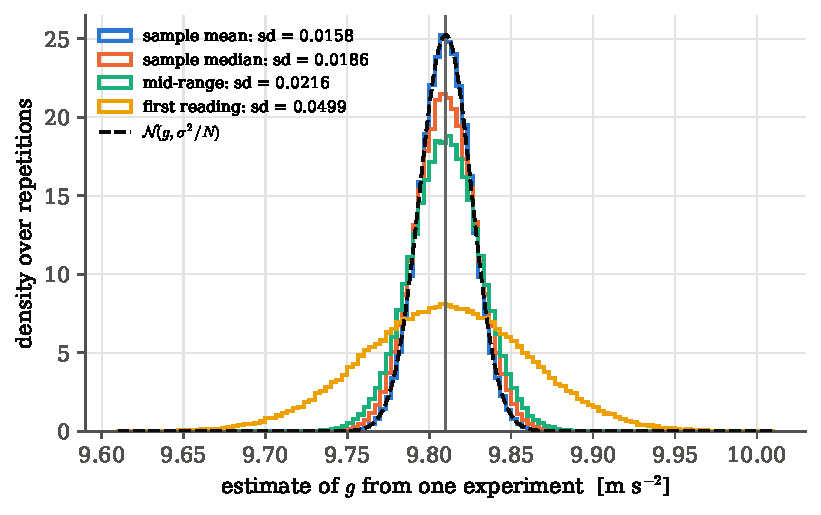
\includegraphics[width=11cm]{figures/ch03/sampling_gauss.pdf}
\caption{Sampling distributions of four estimators of $g$, each built from
the same $\ThreeAM$ simulated ten-reading experiments. All four are centred on
the true value (vertical line). The sample mean is the narrowest and sits on
the derived curve $\Normal(g,\sigma^2/N)$. Using only the first reading gives
a distribution as wide as the noise itself.}
\label{3a:fig:sampling-gauss}
\end{figure}

The numbers: the sample mean scatters by $\ThreeASdMean$ against the derived
$\sigma/\sqrt{N}=\ThreeASdTheory$; the median by $\ThreeASdMedian$ (its
variance is $\ThreeAMedianVarRatio$ times larger, tending to $\pi/2\approx1.57$
for large $N$ with Gaussian noise); the mid-range by $\ThreeASdMidrange$; the
first reading by $\ThreeASdFirst\approx\sigma$. All four recipes are
``right on average''. They differ in how much they scatter, and that is what
makes one of them better. \Cref{3a:sec:bias-variance} makes ``better''
precise.

\begin{figure}[htbp]
\centering
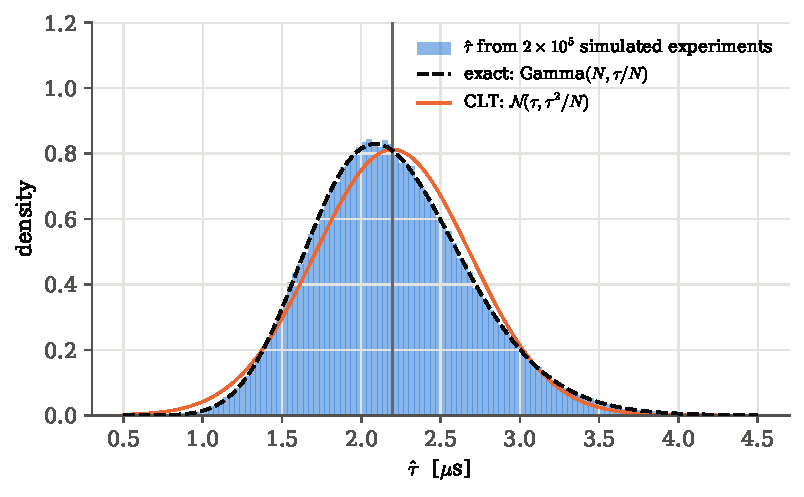
\includegraphics[width=10.5cm]{figures/ch03/sampling_lifetime.pdf}
\caption{Sampling distribution of the lifetime estimate from twenty decays.
The histogram of simulated $\hat\tau$ follows the exact Gamma density
\eqref{3a:eq:gamma-sampling} (dashed), including its longer right tail. The
Gaussian with the same mean and width (solid) is close but visibly too
symmetric.}
\label{3a:fig:sampling-lifetime}
\end{figure}

The simulated mean and spread of $\hat\tau$ are $\ThreeATauMean$ and
$\ThreeATauSd\,\mu$s, against the derived $\tau=2.197$ and
$\tau/\sqrt{20}=0.491\,\mu$s.

\paragraph{What this bought us.}
An estimator is a recipe, so it has a sampling distribution. The standard
error is the width of that distribution, not the width of the data: with ten
readings of noise $\sigma$ the sample mean scatters by $\sigma/\sqrt{10}$, a
single reading by $\sigma$.

\begin{center}\small
\begin{tabularx}{\linewidth}{@{}lXl@{}}
\toprule
word & what it is & pendulum example\\
\midrule
parameter $\theta$ & fixed, unknown number labelling the true distribution & the true $g$\\
statistic & any function of the data with no unknowns & $\max_i x_i$, $\sum x_i^2$\\
estimator $\hat\theta$ & a statistic used to guess $\theta$; a random variable & $\bar X=N^{-1}\sum X_i$\\
estimate & the estimator evaluated on our data; one number & $9.815$\\
standard error & width of the estimator's sampling distribution & $\sigma/\sqrt N=0.016$\\
\bottomrule
\end{tabularx}
\end{center}

\begin{pitfall}[What is random and what is fixed]
In the frequentist picture, $\theta$ is fixed and $\hat\theta$ is
random. A statement such as ``$g=9.815\pm0.016$'' is shorthand for a statement
about the \emph{recipe}: applied to repeated experiments, it lands within
$0.016$ of the truth about two times in three. It is not a probability
distribution for $g$. Probability distributions \emph{for} parameters are the
Bayesian answer of \cref{ch:05}, and the precise meaning of an interval is the
subject of \cref{ch:04}.
\end{pitfall}

\paragraph{A first look at intervals and tests.}
The sampling distribution also gives the two other basic tools of
statistics, intervals and tests. Suppose $\hat\theta_N$ is approximately
Gaussian with estimated standard error $\widehat{\operatorname{se}}$ (the
central limit theorem of \cref{3a:sec:lln-clt} explains why this is so
common). Then the interval
$C_N=(\hat\theta_N-z_{\alpha/2}\widehat{\operatorname{se}},\ \hat\theta_N+z_{\alpha/2}\widehat{\operatorname{se}})$
with $z_{\alpha/2}=\Phi^{-1}(1-\alpha/2)$ ($\Phi$ is the standard normal
distribution function) traps the fixed $\theta$ in a
fraction $1-\alpha$ of repetitions as $N\to\infty$ \mainref{p.~94, Thm~6.16}.
For $\alpha=0.05$, $z_{\alpha/2}=1.96\approx2$: ``estimate $\pm$ two standard
errors''. For the
Bernoulli case the interval is
$\hat p\pm z_{\alpha/2}\sqrt{\hat p(1-\hat p)/N}$ \mainref{Ex.~6.17}.

A \newterm{hypothesis test} uses the same sampling distribution the other
way round. We start from a default hypothesis, such as ``the coin is fair'',
$p=1/2$. Under it we know how $T=|\hat p-1/2|$ is distributed. If the
observed $T$ is larger than the default would usually produce, we reject the
default \mainref{p.~95, Ex.~6.18}. Both ideas are developed properly in
\cref{ch:04}.

\paragraph{Verification and research.}
Here the Monte Carlo \emph{verifies} a result we can derive,
$\operatorname{se}(\bar X)=\sigma/\sqrt N$. The same few lines, ``simulate the
experiment many times, apply the recipe, histogram the output'', are the
\emph{research instrument} when no formula exists. The sampling distribution
of a CMB power spectrum estimated from a masked, noisy, beam-smoothed map
(\cref{ch:08}), or of a topological summary of a field such as its Euler
characteristic (\cref{ch:12}), is obtained in exactly this way, with a
simulator of the sky in place of \pyname{rng.standard_normal}.

\section{Aiming and scattering: bias, variance and mean squared error}
\label{3a:sec:bias-variance}

Charged particles cross a silicon strip detector and leave hits whose
positions along one strip are uniformly spread between $0$ and the strip's
unknown active length $\theta$. We record $n=10$ hit positions. Three
colleagues propose three recipes. The first doubles the average position
(the average of a uniform variable sits in the middle). The second takes
the largest position seen (no hit can be beyond the end). The third takes
the largest position and nudges it up a little, because the largest of ten
hits is almost never exactly at the end.

Which recipe should we use? Each one is a guess at $\theta$, and each guess
misses by some amount that changes from experiment to experiment. The fair
comparison is the average squared miss, the mean squared error. It splits
into two parts every experimentalist already knows: a systematic offset and
a statistical scatter.

\paragraph{Darts at a target.}
Picture the sampling distribution of \cref{3a:sec:sampling} as a cluster of
darts around a bull's-eye at the true value. Two things can go wrong. The
cluster can be centred in the wrong place (a thrower with a consistent pull
to the left), or it can be wide (a shaky hand). The first is \emph{bias}, the
second is \emph{variance}. A good estimator needs both to be small, and it
may be worth accepting a little of one to remove a lot of the other.

\begin{figure}[htbp]
\centering
\begin{tikzpicture}[font=\small]
  \pgfmathsetseed{7}
  \foreach \col/\bx/\s/\ttl [count=\k] in
      {0/0/0.18/{low bias\\ low variance},
       1/0.55/0.18/{high bias\\ low variance},
       2/0/0.55/{low bias\\ high variance},
       3/0.55/0.55/{high bias\\ high variance}}{
    \begin{scope}[xshift=\col*3.3cm]
      \draw[faint] (0,0) circle (1.2);
      \draw[faint] (0,0) circle (0.8);
      \draw[faint] (0,0) circle (0.4);
      \fill[bdryred] (0,0) circle (1.2pt);
      \foreach \i in {1,...,14}{
        \pgfmathsetmacro{\px}{\bx+\s*rand}
        \pgfmathsetmacro{\py}{0.25*\bx+\s*rand}
        \fill[formblue] (\px,\py) circle (1.5pt);
      }
      \node[align=center,font=\footnotesize] at (0,-1.6) {\ttl};
    \end{scope}
  }
\end{tikzpicture}
\caption{Four throwers, fourteen darts each. The red dot is the true value of
the parameter and every blue dot is the estimate from one repetition of the
experiment. Moving the whole cluster off the centre is bias. Spreading it out
is variance. The mean squared error is the average squared distance of the
darts from the red dot, and it grows with both.}
\label{3a:fig:darts}
\end{figure}

\paragraph{The questions, in words.}
\begin{enumerate}[label=\arabic*.]
  \item Over many repetitions, where is the recipe's output centred? Is that
        the true value? (Bias.)
  \item How widely does the output scatter about its own centre? (Variance,
        or its square root, the standard error.)
  \item On average, how far is the output from the \emph{truth}, counting
        both effects? (Mean squared error.)
  \item As we take more data, does the output settle down on the truth?
        (Consistency.)
\end{enumerate}

\subsection{Bias, variance and their sum}
\label{3a:sec:mse}

Two things can be wrong with an estimator: its centre can be off, and its
spread can be large. Each has a name, and the two combine into one measure of
total error.

\begin{workdef}[bias, unbiased, mean squared error]
The \newterm{bias} of an estimator $\hat\theta_n$ is
\begin{equation}
  \operatorname{bias}(\hat\theta_n)=\E_\theta(\hat\theta_n)-\theta
  \label{3a:eq:bias}
\end{equation}
\unpack{the offset of the centre of the sampling distribution from the
truth, at this fixed $\theta$}. The estimator is \newterm{unbiased} if the
bias is zero for \emph{every} $\theta$ in $\Theta$. The \newterm{mean
squared error} is
\begin{equation}
  \operatorname{MSE}(\hat\theta_n)=\E_\theta\bigl[(\hat\theta_n-\theta)^2\bigr]
  \label{3a:eq:mse-def}
\end{equation}
\unpack{the average over repetitions of the squared miss distance}.
\end{workdef}

Both are functions of the unknown $\theta$, because the average is taken
with $f(x;\theta)$. The two ideas fit together exactly: the MSE is the
variance plus the squared bias. To show it, call the centre of the sampling
distribution $\bar\theta_n\defeq\E_\theta(\hat\theta_n)$. It is a fixed
number, not a random variable. Then
\begin{align}
  \operatorname{MSE}(\hat\theta_n)
  &\eqby{1} \E_\theta\bigl[(\hat\theta_n-\bar\theta_n+\bar\theta_n-\theta)^2\bigr]
     \nonumber\\
  &\eqby{2} \E_\theta\bigl[(\hat\theta_n-\bar\theta_n)^2\bigr]
     +2(\bar\theta_n-\theta)\,\E_\theta\bigl[\hat\theta_n-\bar\theta_n\bigr]
     +(\bar\theta_n-\theta)^2 \nonumber\\
  &\eqby{3} \E_\theta\bigl[(\hat\theta_n-\bar\theta_n)^2\bigr]+(\bar\theta_n-\theta)^2
     \nonumber\\
  &\eqby{4} \Var_\theta(\hat\theta_n)+\operatorname{bias}^2(\hat\theta_n).
  \label{3a:eq:mse-decomp}
\end{align}
\begin{explain}
  \item Add and subtract the constant $\bar\theta_n$ inside the square.
  \item Expand $(a+b)^2=a^2+2ab+b^2$ with $a=\hat\theta_n-\bar\theta_n$ (random)
        and $b=\bar\theta_n-\theta$ (constant). Constants come out of the
        expectation, and $\E(b^2)=b^2$.
  \item $\E_\theta[\hat\theta_n-\bar\theta_n]=\bar\theta_n-\bar\theta_n=0$ by the
        definition of $\bar\theta_n$, so the cross term vanishes.
  \item The first term is the variance by definition. The second is the
        squared bias \eqref{3a:eq:bias}.
\end{explain}

\begin{keyidea}[MSE = bias$^2$ + variance]
The mean squared error of any estimator is the square of its systematic
offset plus the square of its statistical scatter,
$\operatorname{MSE}=\operatorname{bias}^2+\operatorname{se}^2$. For an
unbiased estimator the MSE is just the variance.
\end{keyidea}

Why is the result true, beyond the algebra? It is Pythagoras. The miss
$\hat\theta_n-\theta$ is a fixed offset $b$ (the bias) plus a random part
$a$ whose average is zero. Squaring gives $a^2+2ab+b^2$. The cross term
averages to zero, because $b$ is a constant and $a$ averages to zero. So the
two parts add in square, like the two perpendicular sides of a right
triangle. The same identity is the parallel-axis theorem of mechanics: the
moment of inertia about the true value equals the moment about the centre of
mass plus the total mass times the squared distance between the two.

\paragraph{Statistics and the laboratory.}
\begin{center}\small
\begin{tabular}{@{}ll@{}}
\toprule
statistics & laboratory\\
\midrule
bias & systematic error (a miscalibrated scale)\\
standard error & statistical error (shrinks with more data)\\
$\operatorname{MSE}=\operatorname{bias}^2+\operatorname{se}^2$ & ``add the errors in quadrature''\\
unbiased estimator & a method with no systematic offset, for every true value\\
consistent estimator & a method that homes in on the truth as data accumulate\\
\bottomrule
\end{tabular}
\end{center}

The variance of the estimator is the \emph{statistical} error. A bias, or a
mistake in the model, is a \emph{systematic} error, and more data do not
remove it \srcref{Cowan}{\S5.1, (5.5)}. One caution about the quadrature
row. Physicists add a systematic in quadrature because they treat its
unknown size as random, drawn from an ensemble of possible miscalibrations.
The bias in \eqref{3a:eq:mse-decomp} is not random. It is a definite, if
unknown, number, and it enters squared for a purely algebraic reason: the
cross term vanished.

\subsection{Three recipes for the strip length}
\label{3a:sec:uniform}

Back to the silicon strip from the start of this section. A strip of unknown
active length $\theta$ records $n=10$ hits, and each hit position $X_i$ is
equally likely to be anywhere along it, $X_i\sim\mathrm{Uniform}(0,\theta)$,
with density $1/\theta$ on $[0,\theta]$. The three colleagues each proposed a
way of turning the ten positions into one number for $\theta$, that is, an
estimator $\hat\theta=g(X_1,\dots,X_n)$ in the sense of \cref{3a:sec:estimator}.
It is customary to call a candidate estimator $T$ (for a statistic of the data),
and we number the three candidates in the order the colleagues proposed them.
Two ingredients appear in them: the sample mean
$\bar X=\frac1n\sum_{i=1}^nX_i$, and the largest of the ten positions, written
$X_{(n)}=\max_iX_i$ (the subscript in parentheses means ``the $n$-th in order of
size''). The moments of a single hit we need are (from \cref{ch:02})
\begin{equation}
  \E X_i=\frac\theta2,\qquad \E X_i^2=\int_0^\theta\frac{x^2}{\theta}\dd x=\frac{\theta^2}{3},
  \qquad \Var X_i=\frac{\theta^2}{3}-\frac{\theta^2}{4}=\frac{\theta^2}{12}.
  \label{3a:eq:uniform-moments}
\end{equation}
The three recipes, written as formulas, are
\begin{align*}
  T_1&=2\bar X &&\text{double the average position (a uniform hit sits at $\theta/2$ on average),}\\
  T_2&=X_{(n)} &&\text{take the largest position (no hit can lie beyond the end),}\\
  T_3&=\tfrac{n+1}{n}\,X_{(n)} &&\text{nudge the largest position up (it almost never reaches the end).}
\end{align*}
For each recipe we ask the questions listed above: where is it centred, how
widely does it scatter, and what is its total error?

\paragraph{Example: Doubling the mean.}
\label{3a:ex:uniform-mean}
\begin{align*}
  \E T_1 &\eqby{1} 2\cdot\frac1n\sum_{i=1}^n\E X_i \eqby{2} 2\cdot\frac\theta2=\theta,\\
  \Var T_1 &\eqby{3} 4\,\Var\bar X \eqby{4} 4\cdot\frac{\theta^2}{12\,n}=\frac{\theta^2}{3n}.
\end{align*}
\begin{explain}
  \item Linearity of expectation.
  \item Each $\E X_i=\theta/2$ by \eqref{3a:eq:uniform-moments}.
  \item $\Var(cU)=c^2\Var U$ with $c=2$.
  \item $\Var\bar X=\Var X_i/n$ for independent readings (the same steps as in
        \cref{3a:ex:bernoulli}, and derived generally in \eqref{3a:eq:var-mean}).
\end{explain}
So $T_1$ is unbiased and $\operatorname{MSE}(T_1)=\theta^2/(3n)$. For $n=10$
and $\theta=1$ this is $0.0333$.

\paragraph{Example: The largest hit.}
\label{3a:ex:uniform-max}
We first need the sampling distribution of the maximum. The maximum is below
$t$ exactly when \emph{every} hit is below $t$. For $0\le t\le\theta$,
\begin{align*}
  \Prob(X_{(n)}\le t)
  &\eqby{1} \Prob(X_1\le t,\ X_2\le t,\ \dots,\ X_n\le t)
   \eqby{2} \prod_{i=1}^n\Prob(X_i\le t)
   \eqby{3} \Bigl(\frac t\theta\Bigr)^n .
\end{align*}
\begin{explain}
  \item ``The largest is at most $t$'' is the same event as ``all are at most $t$''.
  \item The hits are independent, so the joint probability factorises.
  \item For a uniform variable $\Prob(X_i\le t)=t/\theta$.
\end{explain}
Differentiating, the density is $g(t)=n\,t^{n-1}/\theta^n$ on $[0,\theta]$.
It piles up near the end of the strip, as the picture of ten hits suggests.
Its moments are
\begin{align*}
  \E X_{(n)} &\eqby{1} \int_0^\theta t\cdot\frac{n\,t^{n-1}}{\theta^n}\dd t
    \eqby{2} \frac{n}{\theta^n}\,\frac{\theta^{n+1}}{n+1}=\frac{n}{n+1}\,\theta,\\
  \E X_{(n)}^2 &\eqby{3} \frac{n}{\theta^n}\,\frac{\theta^{n+2}}{n+2}=\frac{n}{n+2}\,\theta^2,\\
  \Var X_{(n)} &\eqby{4} \frac{n}{n+2}\,\theta^2-\frac{n^2}{(n+1)^2}\,\theta^2
    \eqby{5} \frac{n\,\theta^2}{(n+1)^2(n+2)} .
\end{align*}
\begin{explain}
  \item Definition of the mean of a continuous variable with density $g$.
  \item $\int_0^\theta t^n\dd t=\theta^{n+1}/(n+1)$.
  \item The same integral with one more power of $t$: $\int_0^\theta t^{n+1}\dd t=\theta^{n+2}/(n+2)$.
  \item $\Var=\E X^2-(\E X)^2$.
  \item Common denominator: $n(n+1)^2-n^2(n+2)=n\bigl[(n+1)^2-n(n+2)\bigr]=n$.
\end{explain}
So $\operatorname{bias}(T_2)=\frac{n}{n+1}\theta-\theta=-\frac{\theta}{n+1}$:
the largest hit always falls short of the end. By \eqref{3a:eq:mse-decomp},
\begin{align*}
  \operatorname{MSE}(T_2)
  &\eqby{1} \frac{\theta^2}{(n+1)^2}+\frac{n\,\theta^2}{(n+1)^2(n+2)}
   \eqby{2} \frac{\theta^2\,\bigl[(n+2)+n\bigr]}{(n+1)^2(n+2)}
   = \frac{2\,\theta^2}{(n+1)(n+2)} .
\end{align*}
\begin{explain}
  \item Squared bias plus variance.
  \item Put both terms over the denominator $(n+1)^2(n+2)$. Then
        $2n+2=2(n+1)$ cancels one factor of $n+1$.
\end{explain}
For $n=10$: bias $=-1/11=\ThreeAUTwoBiasth$ and
$\operatorname{MSE}=2/132=\ThreeAUTwoMSEth$ (with $\theta=1$). Even though it
is biased, $T_2$ has less than half the MSE of the unbiased $T_1$.

\paragraph{Example: Correcting the bias.}
\label{3a:ex:uniform-corrected}
The bias of $T_2$ is known exactly, as a fraction of $\theta$, so we can
divide it out:
\begin{align*}
  \E T_3 &\eqby{1} \frac{n+1}{n}\,\E X_{(n)} \eqby{2} \frac{n+1}{n}\cdot\frac{n}{n+1}\,\theta=\theta,\\
  \Var T_3 &\eqby{3} \frac{(n+1)^2}{n^2}\cdot\frac{n\,\theta^2}{(n+1)^2(n+2)}
   =\frac{\theta^2}{n(n+2)} .
\end{align*}
\begin{explain}
  \item Linearity, with the constant $(n+1)/n$.
  \item The mean of the maximum from \cref{3a:ex:uniform-max}.
  \item $\Var(cU)=c^2\Var U$ with $c=(n+1)/n$, and the variance of the maximum.
\end{explain}
Now $\operatorname{MSE}(T_3)=\theta^2/(n(n+2))=1/120=\ThreeAUThreeMSEth$ for
$n=10$: unbiased \emph{and} four times better than $T_1$. For large $n$,
$\operatorname{MSE}(T_1)\propto1/n$ while $\operatorname{MSE}(T_3)\propto1/n^2$.
The maximum uses the one feature of the data (the sharp edge) that carries
the most information about $\theta$. The mean washes that edge out.

\paragraph{Seeing it in Python.}
\Cref{3a:lst:uniform} simulates $M=200\,000$ experiments of ten hits and
applies all three recipes to each.

\pyfile[firstline=24,lastline=36,label={3a:lst:uniform}]{code/ch03/02_bias_variance_uniform.py}{The three recipes and their derived bias and variance}

The function \pyname{estimators} takes a matrix whose rows are experiments
and returns the three estimates for each row. The function \pyname{theory}
encodes the formulas just derived, so the script can put the two side by
side. The simulated biases are $\ThreeAUOneBias$, $\ThreeAUTwoBias$ and
$\ThreeAUThreeBias$ (derived: $0$, $\ThreeAUTwoBiasth$, $0$). The simulated
MSEs are $\ThreeAUOneMSE$, $\ThreeAUTwoMSE$ and $\ThreeAUThreeMSE$ (derived:
$\ThreeAUOneMSEth$, $\ThreeAUTwoMSEth$, $\ThreeAUThreeMSEth$). Agreement to
the third digit is what $M=200\,000$ repetitions buy.

\begin{figure}[htbp]
\centering
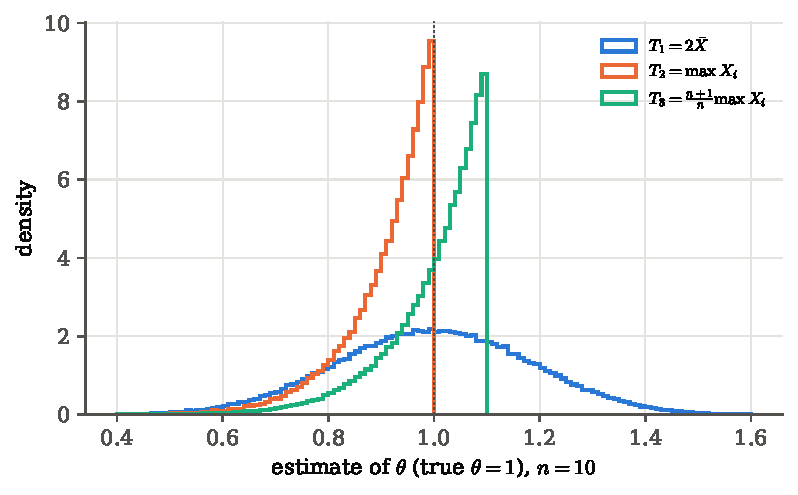
\includegraphics[width=11cm]{figures/ch03/uniform_estimators.pdf}
\caption{Sampling distributions of the three strip-length recipes with ten
hits each. Doubling the mean gives a broad, symmetric bump centred on the
truth. The largest hit gives a sharp distribution that ends exactly at the
truth and so sits entirely to its left. Stretching it by $11/10$ moves it
onto the truth and keeps it narrow.}
\label{3a:fig:uniform-estimators}
\end{figure}

\begin{figure}[htbp]
\centering
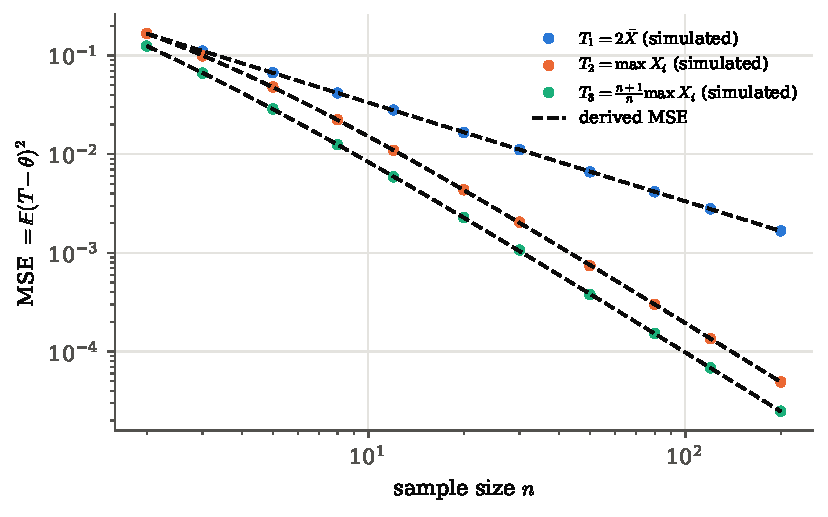
\includegraphics[width=10.5cm]{figures/ch03/uniform_mse.pdf}
\caption{Mean squared error against the number of hits, on log--log axes.
The points are simulations and the dashed curves the derived formulas.
Doubling the mean falls with slope $-1$. Both recipes built on the largest
hit fall with slope $-2$, and the corrected one stays below the uncorrected
one at every $n$.}
\label{3a:fig:uniform-mse}
\end{figure}

\subsection{The MSE depends on the truth}
\label{3a:sec:mse-theta}

For the strip, $T_3$ beat $T_1$ at every $\theta$. That is unusual. The MSE
is a function of the unknown truth, so one recipe can win for some true
values and lose for others. The simplest case shows how.

\paragraph{Example: Shrinking the mean towards zero.}
\label{3a:ex:shrinkage}
Let $X_1,\dots,X_n\sim\Normal(\mu,\sigma^2)$ and consider the family of
recipes $T_c=c\,\bar X$ with a constant $0<c\le1$. Then
\begin{align*}
  \operatorname{MSE}(T_c)
  &\eqby{1} \bigl(\E T_c-\mu\bigr)^2+\Var T_c
   \eqby{2} (c-1)^2\mu^2+c^2\,\frac{\sigma^2}{n}.
\end{align*}
\begin{explain}
  \item The decomposition \eqref{3a:eq:mse-decomp}.
  \item $\E T_c=c\mu$ and $\Var T_c=c^2\Var\bar X=c^2\sigma^2/n$.
\end{explain}
Setting the derivative with respect to $c$ to zero,
$2(c-1)\mu^2+2c\,\sigma^2/n=0$, gives the best constant
$c^\ast=\mu^2/(\mu^2+\sigma^2/n)$. It depends on the unknown $\mu$, so it is
not a recipe we can use. Fix $c<1$ instead and compare with $\bar X$, which
is $T_1$ here and has MSE $\sigma^2/n$. Shrinking lowers the variance term
by the factor $c^2$ but adds the bias term $(c-1)^2\mu^2$, which grows with
$\mu$. So shrinking wins when $\mu$ is near zero and loses when $\mu$ is far
from zero (\cref{3a:fig:mse-crossing}). With $\sigma^2/n=1$ and $c=0.8$ the
curves cross where $0.04\,\mu^2+0.64=1$, i.e.\ at $|\mu|=3$.

\begin{figure}[htbp]
\centering
\begin{tikzpicture}
\begin{axis}[width=9.5cm,height=5.4cm,xmin=-5,xmax=5,ymin=0,ymax=2.2,
  xlabel={true mean $\mu$ (in units of $\sigma/\sqrt n$)},
  ylabel={MSE (units of $\sigma^2/n$)},
  legend style={font=\footnotesize,at={(0.5,0.97)},anchor=north},
  tick label style={font=\footnotesize},label style={font=\small}]
  \addplot[very thick,formblue,domain=-5:5] {1};
  \addlegendentry{$\bar X$ (unbiased)}
  \addplot[very thick,fibreorange,domain=-5:5,samples=101] {0.04*x^2+0.64};
  \addlegendentry{$0.8\,\bar X$ (biased)}
  \draw[faint,dashed] (axis cs:3,0) -- (axis cs:3,1);
  \draw[faint,dashed] (axis cs:-3,0) -- (axis cs:-3,1);
  \fill[bdryred] (axis cs:3,1) circle (1.6pt);
  \fill[bdryred] (axis cs:-3,1) circle (1.6pt);
\end{axis}
\end{tikzpicture}
\caption{Mean squared error of two recipes for a Gaussian mean, as a function
of the true value. The sample mean has the same MSE everywhere. The shrunken
recipe wins inside $|\mu|<3$ and loses outside, and the two curves meet at the
red dots. Neither is better for every possible truth.}
\label{3a:fig:mse-crossing}
\end{figure}

\paragraph{There is usually no ``best'' estimator.}
Because the MSE is a function of $\theta$, two estimators are usually not
ordered: one wins for some true values and loses for others. The simplest
way to get a meaningful comparison is to restrict the class, for instance
to unbiased estimators, and look for the smallest variance inside it. That
programme leads to the Cram\'er--Rao bound and the Fisher information
(second half of \cref{ch:03} and \cref{ch:10}).

\begin{pitfall}[Unbiased is not the same as good]
An unbiased estimator can be much worse than a biased one. $T_1$ in the strip
example is unbiased and has four times the MSE of $T_3$ and twice that of
the biased $T_2$. Conversely, a biased estimator is not ``wrong'': Wasserman
notes that unbiasedness ``used to receive much attention but these days is
considered less important'' \mainref{p.~90}. What matters is the size of
the total error, and that it shrinks as data accumulate.
\end{pitfall}

\paragraph{Example: Poisson counts.}
\label{3a:ex:poisson}
A counter records $X_1,\dots,X_n\sim\mathrm{Poisson}(\lambda)$ events in $n$
equal time bins, and we estimate the rate by $\hat\lambda=\bar X$. From
\cref{ch:02}, $\E X_i=\Var X_i=\lambda$. Then
\begin{align*}
  \operatorname{bias}(\hat\lambda) &\eqby{1} \frac1n\sum_i\E X_i-\lambda=0,\\
  \operatorname{se}(\hat\lambda) &\eqby{2} \sqrt{\frac{\Var X_i}{n}}=\sqrt{\frac\lambda n},\\
  \operatorname{MSE}(\hat\lambda) &\eqby{3} 0^2+\frac\lambda n=\frac\lambda n .
\end{align*}
\begin{explain}
  \item Linearity and $\E X_i=\lambda$.
  \item Variance of a mean of independent readings, and $\Var X_i=\lambda$ for a Poisson variable.
  \item Decomposition \eqref{3a:eq:mse-decomp} with zero bias.
\end{explain}
The estimated standard error is $\sqrt{\hat\lambda/n}$. For $n=1$ this is the
familiar ``$\sqrt N$ error on $N$ counts'' \mainref{Exercise~6.1}.

\subsection{Consistency: does the recipe home in on the truth?}
\label{3a:sec:consistency}

A minimal demand on any recipe is that more data make it better, eventually
without limit. To say this precisely we must say what it means for a
sequence of random numbers to approach a constant. One random number can
still land anywhere, so ``approach'' has to be a statement about
probabilities. The simplest version is below (the other versions are in
\cref{3a:sec:convergence}).

\paragraph{Convergence in probability and consistency.}
A sequence of random variables $Y_n$ \newterm{converges in probability} to a
constant $c$, written $Y_n\xrightarrow{\;P\;}c$, if for every $\epsilon>0$
\begin{equation}
  \Prob\bigl(|Y_n-c|>\epsilon\bigr)\;\longrightarrow\;0\qquad(n\to\infty)
  \label{3a:eq:conv-prob}
\end{equation}
\unpack{any band around $c$, however narrow, eventually contains $Y_n$ in
almost all repetitions}. An estimator is \newterm{consistent} if
$\hat\theta_n\xrightarrow{P}\theta$ for every $\theta\in\Theta$.

To prove consistency we need a bound on the probability of a large miss.
One elementary inequality supplies it.

\paragraph{Markov and Chebyshev inequalities.}
If $Y\ge0$ and $t>0$, then $\Prob(Y\ge t)\le\E Y/t$ (Markov). Applied to
$Y=(U-a)^2$ with $t=\epsilon^2$ it gives, for any random variable $U$ and
any constant $a$,
\begin{equation}
  \Prob\bigl(|U-a|\ge\epsilon\bigr)\le\frac{\E\bigl[(U-a)^2\bigr]}{\epsilon^2}.
  \label{3a:eq:chebyshev}
\end{equation}
With $a=\E U$ the numerator is $\Var U$ (Chebyshev).

Markov's inequality is true for a reason we can see: a non-negative
quantity cannot have a big chunk of probability at large values without
dragging its average up. Written out, with $\mathbb{1}\{\cdot\}$ the
indicator that is $1$ when the condition holds and $0$ otherwise,
\begin{align}
  \E Y
  &\relby{1}{\ge} \E\bigl[Y\,\mathbb{1}\{Y\ge t\}\bigr]
   \relby{2}{\ge} \E\bigl[t\,\mathbb{1}\{Y\ge t\}\bigr]
   \eqby{3} t\,\Prob(Y\ge t).
  \label{3a:eq:markov}
\end{align}
\begin{explain}
  \item $Y\ge0$, so throwing away the part of the average where $Y<t$ cannot increase it.
  \item Where the indicator is $1$, $Y\ge t$. Where it is $0$, both sides are $0$.
  \item The average of an indicator is the probability of its event.
\end{explain}
Dividing by $t$ gives Markov. Now take $U=\hat\theta_n$ and $a=\theta$ in
\eqref{3a:eq:chebyshev}: the numerator is exactly the MSE, so
\begin{equation}
  \Prob\bigl(|\hat\theta_n-\theta|\ge\epsilon\bigr)
  \le\frac{\operatorname{MSE}(\hat\theta_n)}{\epsilon^2}
  =\frac{\operatorname{bias}^2(\hat\theta_n)+\operatorname{se}^2(\hat\theta_n)}{\epsilon^2}.
  \label{3a:eq:mse-consistency}
\end{equation}

\paragraph{A sufficient condition for consistency.}
If $\operatorname{bias}(\hat\theta_n)\to0$ and
$\operatorname{se}(\hat\theta_n)\to0$ as $n\to\infty$, then $\hat\theta_n$ is
consistent. The reason is \eqref{3a:eq:mse-consistency}: its right side then
goes to zero for every fixed $\epsilon$, and it bounds the probability of a
miss larger than $\epsilon$.

\paragraph{Example: Which recipes are consistent?}
\label{3a:ex:consistency}
\begin{itemize}
  \item $\hat p=\bar X$ for coin flips: bias $0$, $\operatorname{se}=\sqrt{p(1-p)/n}\to0$.
        Consistent \mainref{Ex.~6.11}.
  \item $T_2=X_{(n)}$ for the strip: bias $-\theta/(n+1)\to0$, variance
        $\sim\theta^2/n^2\to0$. \emph{Biased but consistent.}
  \item ``Use the first reading only'' for the pendulum: bias $0$ but
        $\operatorname{se}=\sigma$ for every $n$. The inequality tells us
        nothing, and indeed $\Prob(|X_1-g|>\epsilon)$ is the same fixed
        number for all $n$. \emph{Unbiased but not consistent.}
\end{itemize}
Bias and consistency are therefore independent properties. One is about
the centre of the sampling distribution at fixed $n$, the other about the
whole distribution as $n\to\infty$.

\paragraph{Try it.}
Show that $T_c=c_n\bar X$ with $c_n=n/(n+1)$ is biased for every finite $n$
and yet consistent for a Gaussian mean. (Compute its bias and variance and
let $n\to\infty$.)

\paragraph{What this bought us.}
Choose recipes by their total error, $\operatorname{MSE}=\operatorname{bias}^2
+\operatorname{se}^2$. Bias alone is a poor guide. A recipe whose bias and
standard error both vanish as the data grow is consistent, by Chebyshev's
inequality.

\paragraph{Verification and research.}
For the strip we could derive every number, and the simulation only checked
the algebra. In real analyses the recipe is often a long chain (a fit
inside a selection inside a reconstruction) and the bias has no formula. The
standard remedy is the same simulation used as an instrument: inject a known
truth into simulated data, run the full chain many times, and measure the
bias and scatter of the output. This ``injection--recovery'' test is how
the bias of a CMB power spectrum estimator on a masked sky is found and
removed (\cref{ch:08}).

\section{Why error bars shrink like $1/\sqrt N$: the law of large numbers and the central limit theorem}
\label{3a:sec:lln-clt}

Every accelerator physicist knows the rule of thumb: to halve the error on
a cross-section, collect four times the luminosity. A Monte Carlo
integration that gives two correct digits with $10^4$ samples needs $10^6$
for three. The rule has exceptions that bite. The average of energies
drawn from a Breit--Wigner resonance does not improve at all as we add
events.

Two theorems account for the rule and for its exceptions. The law of large
numbers says that an average settles on the true mean. The central limit
theorem says how it is distributed on the way: as a Gaussian of width
$\sigma/\sqrt N$, provided the readings have a finite variance $\sigma^2$.
The Breit--Wigner has none, and that is why it escapes the rule.

\paragraph{A random walk, rescaled.}
The sum of $N$ independent readings is a random walk of $N$ steps. Its
distance from the expected position grows like $\sqrt N$, the familiar
result from diffusion ($\langle x^2\rangle\propto t$). The mean is the sum
divided by $N$, so its scatter is $\sqrt N/N=1/\sqrt N$. And the shape of a
diffusing cloud forgets the shape of the individual step: after many steps
it is a Gaussian, whatever the kick distribution was. That is the central
limit theorem, the same statement as the approach of a diffusion kernel to
a heat-equation Gaussian.

\paragraph{What we want to know.}
\begin{enumerate}[label=\arabic*.]
  \item How does the scatter of an average depend on the number of readings,
        and on correlations between them?
  \item In what sense does a random average ``tend to'' the true mean? (There
        are several inequivalent senses.)
  \item What does the histogram of averages look like for large $N$, and how
        large is large?
  \item What breaks, and why, when the parent has no finite variance?
\end{enumerate}

\subsection{The variance of a sum and of a mean}
\label{3a:sec:var-mean}

The $1/\sqrt N$ comes from one identity: the variance of a sum is the sum of
all the variances and covariances of its terms. Let $X_1,\dots,X_N$ have
means $\mu_i$, variances $\sigma_i^2$ and covariances
$\Cov(X_i,X_j)=\E[(X_i-\mu_i)(X_j-\mu_j)]$, with $\Cov(X_i,X_i)=\sigma_i^2$.
For the sum,
\begin{align}
  \Var\Bigl(\sum_{i=1}^NX_i\Bigr)
  &\eqby{1} \E\Bigl[\Bigl(\sum_{i=1}^N(X_i-\mu_i)\Bigr)^2\Bigr]
   \eqby{2} \E\Bigl[\sum_{i=1}^N\sum_{j=1}^N(X_i-\mu_i)(X_j-\mu_j)\Bigr] \nonumber\\
  &\eqby{3} \sum_{i=1}^N\sum_{j=1}^N\Cov(X_i,X_j)
   \eqby{4} \sum_{i=1}^N\sigma_i^2+\sum_{i\neq j}\Cov(X_i,X_j) .
  \label{3a:eq:var-sum}
\end{align}
\begin{explain}
  \item By linearity the mean of the sum is $\sum\mu_i$. The variance is the
        mean squared deviation from it.
  \item The square of a sum is the double sum of all products.
  \item Linearity of expectation, term by term, and the definition of covariance.
  \item Split the double sum into the diagonal $i=j$ and the rest.
\end{explain}
If the readings are independent, every covariance with $i\neq j$ vanishes.
If they also share one variance $\sigma^2$, the mean $\bar X=N^{-1}\sum X_i$
has
\begin{equation}
  \E\bar X=\mu,\qquad
  \Var\bar X=\frac1{N^2}\,N\sigma^2=\frac{\sigma^2}{N},\qquad
  \operatorname{se}(\bar X)=\frac{\sigma}{\sqrt N}
  \label{3a:eq:var-mean}
\end{equation}
\mainref{p.~52, Thm.~3.17}, \srcref{Cowan}{(5.8), (5.13)}. This is the
$1/\sqrt N$. It needs nothing about the parent except a finite $\sigma$.

\paragraph{Example: Averaging a die.}
\label{3a:ex:dice}
For a fair die, $\E X=3.5$ and $\E X^2=(1+4+9+16+25+36)/6=91/6$, so
$\Var X=91/6-49/4=35/12=2.917$. The average of $50$ rolls therefore has
$\Var\bar X=2.917/50=0.0583$ and $\operatorname{se}=0.24$
\srcref{SeeingTheory}{pp.~38--39}. The individual rolls scatter over
$1$--$6$, their average over roughly $3.26$--$3.74$ (two thirds of the time).

\paragraph{Example: Correlated readings do not average away.}
\label{3a:ex:correlated-mean}
Suppose every pair of readings has the same correlation $\rho$, so
$\Cov(X_i,X_j)=\rho\sigma^2$ for $i\neq j$. This happens when a common
drift, such as a temperature change in the pendulum lab, moves all readings
together. There are $N(N-1)$ ordered pairs with $i\neq j$, so from
\eqref{3a:eq:var-sum}
\begin{align*}
  \Var\bar X
  &\eqby{1} \frac1{N^2}\Bigl[N\sigma^2+N(N-1)\rho\sigma^2\Bigr]
   \eqby{2} \frac{\sigma^2}{N}\bigl[1+(N-1)\rho\bigr]
   \;\xrightarrow{N\to\infty}\;\rho\,\sigma^2 .
\end{align*}
\begin{explain}
  \item Divide the variance of the sum by $N^2$. Diagonal terms give $N\sigma^2$, off-diagonal ones $N(N-1)\rho\sigma^2$.
  \item Factor out $\sigma^2/N$.
\end{explain}
With $\rho=0.1$ the error of the mean can never fall below
$\sqrt{0.1}\,\sigma=0.32\,\sigma$, however many readings we take. The ratio
$N_{\mathrm{eff}}=\sigma^2/\Var\bar X=N/[1+(N-1)\rho]$ is the number of
\emph{effectively independent} readings. The same quantity decides how
useful a correlated Markov chain is (\cref{ch:09}).

\subsection{What ``tends to'' means for random variables}
\label{3a:sec:convergence}

For numbers, $a_n\to a$ has one meaning. For random variables there are
several. A random variable is not one number: it is a rule that assigns a
value to every outcome of the experiment, and that rule has a distribution.
A sequence can approach its limit value by value, or only in its
distribution, and these are different things. Two simple sequences show the
difference \mainref{p.~71}. If $X_n\sim\Normal(0,1)$ for every $n$, independently, the
$X_n$ never settle anywhere, yet every one has the same distribution. If
$X_n\sim\Normal(0,1/n)$, the distributions squeeze onto $0$
(\cref{3a:fig:squeeze}), and we would like to say $X_n\to0$.

\begin{workdef}[three modes of convergence]
Let $X_n$ be random variables with distribution functions $F_n$, and $X$ a
random variable with distribution function $F$.
\begin{itemize}
  \item $X_n\xrightarrow{P}X$ (\newterm{in probability}) if
        $\Prob(|X_n-X|>\epsilon)\to0$ for every $\epsilon>0$
        \unpack{the chance of a miss bigger than $\epsilon$ dies out}.
  \item $X_n\rightsquigarrow X$ (\newterm{in distribution}) if
        $F_n(t)\to F(t)$ at every $t$ where $F$ is continuous \unpack{only the
        histograms converge, not the values themselves}.
  \item $X_n\xrightarrow{\text{qm}}X$ (\newterm{in quadratic mean}) if
        $\E(X_n-X)^2\to0$ \unpack{the mean squared miss dies out}.
\end{itemize}
\end{workdef}

\begin{figure}[htbp]
\centering
\begin{tikzpicture}
\begin{axis}[width=10cm,height=5cm,xmin=-3,xmax=3,ymin=0,ymax=4.3,
  xlabel={$x$},ylabel={density of $X_n$},samples=201,
  legend style={font=\footnotesize,draw=none,fill=none},legend pos=north east,
  tick label style={font=\footnotesize},label style={font=\small}]
  \addplot[thick,formblue!45,domain=-3:3] {exp(-x^2/2)/sqrt(2*pi)};
  \addlegendentry{$n=1$}
  \addplot[thick,formblue!70,domain=-3:3] {sqrt(10)*exp(-10*x^2/2)/sqrt(2*pi)};
  \addlegendentry{$n=10$}
  \addplot[thick,formblue,domain=-3:3] {sqrt(100)*exp(-100*x^2/2)/sqrt(2*pi)};
  \addlegendentry{$n=100$}
\end{axis}
\end{tikzpicture}
\caption{The densities of $X_n\sim\Normal(0,1/n)$ for $n=1,10,100$. The area
stays one while the width shrinks like $1/\sqrt n$, so all the probability
crowds onto the point $0$. This is the picture behind every mode of
convergence to a constant.}
\label{3a:fig:squeeze}
\end{figure}

\paragraph{Example: $X_n\sim\Normal(0,1/n)$ converges to $0$ in every sense.}
\label{3a:ex:squeeze}
In quadratic mean, $\E X_n^2=\Var X_n=1/n\to0$. In probability, by
Chebyshev \eqref{3a:eq:chebyshev}, $\Prob(|X_n|>\epsilon)\le1/(n\epsilon^2)\to0$.
In distribution, write $Z=\sqrt n X_n\sim\Normal(0,1)$ with distribution
function $\Phi$:
\begin{align*}
  F_n(t)=\Prob(X_n\le t)
  &\eqby{1} \Prob(\sqrt n X_n\le\sqrt n\,t)
   \eqby{2} \Phi(\sqrt n\,t)
   \;\xrightarrow{n\to\infty}\;
   \begin{cases}0,& t<0,\\ 1/2,& t=0,\\ 1,& t>0.\end{cases}
\end{align*}
\begin{explain}
  \item Multiply both sides of the inequality by $\sqrt n>0$.
  \item $\sqrt nX_n$ is standard normal.
\end{explain}
The limit $X=0$ (a point mass) has $F(t)=0$ for $t<0$ and $F(t)=1$ for
$t\ge0$. The two agree everywhere except at $t=0$, where
$F_n(0)=1/2\neq F(0)=1$. That one disagreement is not a failure of $X_n$ to
approach $0$. At $t=0$ the limit $F$ jumps from $0$ to $1$, and each $X_n$,
being symmetric about $0$, keeps exactly half its probability below the
jump. This is why the definition asks for convergence only where $F$ is
continuous: the jump points of $F$ are ignored \mainref{Ex.~5.3}.

\paragraph{How the modes are related.}
Quadratic mean implies in probability, which implies in distribution. The
converse implications fail in general. There is one important partial
converse: convergence in distribution \emph{to a constant} implies
convergence in probability to that constant \mainref{Thm.~5.4}.

\begin{figure}[htbp]
\centering
\begin{tikzcd}[column sep=huge,row sep=large]
  X_n\xrightarrow{\text{qm}}X \arrow[r,Rightarrow,shift left=3]
  & X_n\xrightarrow{P}X \arrow[r,Rightarrow,shift left=3]
      \arrow[l,Rightarrow,shift left=3,dashed,color=bdryred]
  & X_n\rightsquigarrow X
      \arrow[l,Rightarrow,shift left=3,dashed,color=bdryred]
\end{tikzcd}
\caption{Implications between the modes of convergence. The solid arrows
always hold. The dashed red arrows, pointing back, fail in general. The
dashed arrow from distribution back to probability does hold in one case:
when the limit is a single number, which is the case for consistency.}
\label{3a:fig:modes}
\end{figure}

Why each arrow holds, and why the reverse ones fail:
\begin{itemize}
  \item \emph{qm $\Rightarrow$ P.} Chebyshev with $U=X_n$, $a=X$:
        $\Prob(|X_n-X|>\epsilon)\le\E(X_n-X)^2/\epsilon^2\to0$. This is the
        argument of \eqref{3a:eq:mse-consistency}.
  \item \emph{P $\not\Rightarrow$ qm.} Let $U\sim\mathrm{Uniform}(0,1)$ and
        $X_n=\sqrt n$ if $U<1/n$, else $0$. Then
        $\Prob(|X_n|>\epsilon)=1/n\to0$, but $\E X_n^2=n\cdot(1/n)=1$ for
        every $n$. A rare but large value keeps the mean square alive. The
        same device with $X_n=n^2$ on probability $1/n$ gives
        $X_n\xrightarrow{P}0$ while $\E X_n=n\to\infty$: convergence in
        probability says nothing about averages \mainref{p.~75}.
  \item \emph{P $\Rightarrow$ D.} If $X_n$ is very probably within $\epsilon$
        of $X$, then $\Prob(X_n\le t)$ is squeezed between
        $\Prob(X\le t-\epsilon)$ and $\Prob(X\le t+\epsilon)$ up to a vanishing
        error. At a continuity point both bounds tend to $F(t)$ as
        $\epsilon\to0$.
  \item \emph{D $\not\Rightarrow$ P.} Let $X\sim\Normal(0,1)$ and $X_n=-X$.
        Every $X_n$ has the distribution $\Normal(0,1)$, so $X_n\rightsquigarrow X$
        trivially, but $|X_n-X|=2|X|$ never shrinks.
\end{itemize}

Convergence in probability and in distribution survive the usual
operations \mainref{Thm.~5.5}: if $X_n\xrightarrow{P}X$ and
$Y_n\xrightarrow{P}Y$ then $X_n+Y_n\xrightarrow{P}X+Y$,
$X_nY_n\xrightarrow{P}XY$, and $h(X_n)\xrightarrow{P}h(X)$ for continuous $h$.
For convergence in distribution the analogous rule is \newterm{Slutsky's
theorem}: if $X_n\rightsquigarrow X$ and $Y_n\rightsquigarrow c$, a
\emph{constant}, then $X_n+Y_n\rightsquigarrow X+c$ and
$X_nY_n\rightsquigarrow cX$. (Without the constant it fails: $X_n$ and
$Y_n$ could each be $\Normal(0,1)$ but perfectly anticorrelated, so that
$X_n+Y_n=0$.)

There are two further modes: \emph{almost sure} convergence,
$\Prob(X_n\to X)=1$, which asks for convergence along each single sequence
of outcomes, and convergence in mean, $\E|X_n-X|\to0$. Only the first is
needed, once, for the strong law below.

\subsection{The law of large numbers}
\label{3a:sec:lln}

\paragraph{Weak law of large numbers.}
If $X_1,X_2,\dots$ are iid with mean $\mu$, then
$\bar X_N\xrightarrow{P}\mu$. The distribution of the sample mean piles up
on the true mean.

With a finite variance the proof is one line of Chebyshev
\eqref{3a:eq:chebyshev} with $U=\bar X_N$, $a=\mu$:
\begin{align}
  \Prob\bigl(|\bar X_N-\mu|>\epsilon\bigr)
  &\relby{1}{\le} \frac{\Var\bar X_N}{\epsilon^2}
   \eqby{2} \frac{\sigma^2}{N\epsilon^2}
   \;\xrightarrow{N\to\infty}\;0 .
  \label{3a:eq:wlln}
\end{align}
\begin{explain}
  \item Chebyshev's inequality, with $\E\bar X_N=\mu$ so that the numerator is the variance.
  \item Variance of the mean \eqref{3a:eq:var-mean}.
\end{explain}
The theorem holds even without a finite variance, provided $\E|X|<\infty$
\mainref{Thm.~5.6}. The \emph{strong} law says more: with probability one,
the running average of a single infinite sequence of readings converges to
$\mu$ \mainref{Thm.~5.18}. That is the version that justifies computing an
average along one long Monte Carlo run or one long Markov chain.

The law of large numbers is also a statement about the meaning of
probability. Let $X_i=\mathbb{1}\{\text{event }A\text{ on trial }i\}$. Then
$\bar X_N$ is the relative frequency of $A$ and $\mu=\Prob(A)$, so relative
frequencies converge to probabilities. The ``frequentist'' reading of
probability rests on this.

\paragraph{Example: How many tosses? Chebyshev against the truth.}
\label{3a:ex:coin-chebyshev}
For a fair coin, how large must $n$ be so that
$\Prob(0.4\le\bar X_n\le0.6)\ge0.7$? With $\mu=1/2$ and
$\Var\bar X_n=p(1-p)/n=1/(4n)$,
\begin{align*}
  \Prob(0.4\le\bar X_n\le0.6)
  &\eqby{1} 1-\Prob\bigl(|\bar X_n-\tfrac12|>0.1\bigr)
   \relby{2}{\ge} 1-\frac{1}{4n\,(0.1)^2}
   = 1-\frac{25}{n}.
\end{align*}
\begin{explain}
  \item The complement of ``within $0.1$ of $1/2$''.
  \item Chebyshev with $\Var\bar X_n=1/(4n)$ and $\epsilon=0.1$.
\end{explain}
The bound exceeds $0.7$ once $25/n\le0.3$, i.e.\ $n\ge84$ \mainref{Ex.~5.7}.
Chebyshev is a guarantee for \emph{every} distribution with this variance,
so it is pessimistic for any particular one. The exact binomial probability
at $n=84$ is $\ThreeACoinExact$. Using the Gaussian approximation of the next
subsection, $\Prob(|\bar X_n-\tfrac12|\le0.1)\approx2\Phi(0.1\sqrt n/0.5)-1\ge0.7$
requires $0.2\sqrt n\ge z_{0.85}=\ThreeAZeightyfive$, i.e.\
$n\ge\ThreeACoinNclt$, where the exact probability is $\ThreeACoinExactNclt$.

\paragraph{A sharper guarantee, and a first interval.}
Chebyshev uses only the variance, so it must hold for every distribution.
For Bernoulli readings (each $X_i$ is $0$ or $1$, with $\Prob(X_i=1)=p$) we
know more, and \newterm{Hoeffding's inequality} uses it:
$\Prob(|\bar X_n-p|>\epsilon)\le2e^{-2n\epsilon^2}$ \mainref{Thm.~4.5, (4.4)}.
This bound falls exponentially in $n$, not as $1/n$. With $n=100$ and
$\epsilon=0.2$ it gives $2e^{-8}=0.00067$, where Chebyshev gives only
$1/(4\cdot100\cdot0.04)=0.0625$ \mainref{Ex.~4.6}. (For the moderate
$\epsilon=0.1$ of the coin example, Chebyshev happens to be the stronger of
the two.)

The bound also gives an interval. Set the right side equal to a small
probability $\alpha$ and solve for $\epsilon$:
$\epsilon_n=\sqrt{\ln(2/\alpha)/(2n)}$. Then the interval $\hat p\pm\epsilon_n$
contains the true $p$ with probability at least $1-\alpha$, for \emph{every}
$p$ and every $n$, with no large-$n$ approximation \mainref{Ex.~6.15}. For
$\alpha=0.05$ and $n=100$, $\epsilon_n=\sqrt{3.689/200}=0.136$.

What does ``with probability at least $1-\alpha$'' refer to? Not to $p$,
which is fixed. It refers to the interval recipe, applied over repeated
experiments. A striking case makes the point: Wasserman's Ex.~6.14 builds a
legitimate 75\% interval that, on some data sets, is known with certainty to
contain $\theta$. So the sentence ``with probability 0.95, $p$ is contained
in the interval'', said of $\bar X\pm1.96\,S/\sqrt n$
\srcref{SeeingTheory}{p.~42}, is loose: the $0.95$ belongs to the recipe,
not to $p$. The full story of intervals is in \cref{ch:04}.

\subsection{The central limit theorem}
\label{3a:sec:clt}

The law of large numbers says where the sample mean goes. It does not say
how $\bar X_N$ is distributed on the way, which is what we need for error
bars. The central limit theorem does.

\begin{keyidea}[Central limit theorem]
Let $X_1,\dots,X_N$ be iid with mean $\mu$ and finite variance $\sigma^2$.
Then
\begin{equation}
  Z_N\defeq\frac{\bar X_N-\mu}{\sqrt{\Var\bar X_N}}=\frac{\sqrt N(\bar X_N-\mu)}{\sigma}
  \;\rightsquigarrow\;\Normal(0,1),
  \label{3a:eq:clt}
\end{equation}
that is, $\Prob(Z_N\le z)\to\Phi(z)$ for every $z$. Informally,
$\bar X_N\approx\Normal(\mu,\sigma^2/N)$ whatever the parent distribution.
\end{keyidea}

The theorem approximates probabilities, not values: ``it's the probability
statements that we are approximating, not the random variable itself''
\mainref{p.~77}. No single $\bar X_N$ becomes a Gaussian number; what becomes
Gaussian is the chance that $\bar X_N$ falls in a given range.

In practice we do not know $\sigma$. The theorem still holds with $\sigma$
replaced by the sample standard deviation $S_N$ of
\cref{3a:sec:sample-variance}. The reason: $S_N\xrightarrow{P}\sigma$, and
Slutsky's theorem lets us swap a factor that tends to a constant
\mainref{Thm.~5.10}. For random vectors,
$\sqrt N(\bar{\bm X}_N-\bm\mu)\rightsquigarrow\Normal(\bm 0,\bm\Sigma)$ with
$\bm\Sigma$ the covariance matrix of one reading \mainref{Thm.~5.12}.

\paragraph{Why it is true: cumulants add.}
The cleanest physicist's argument uses the \newterm{cumulant generating
function} $K_Y(t)=\ln\E\,e^{tY}=\sum_{k\ge1}\kappa_k t^k/k!$, the logarithm
of the moment generating function. Its Taylor coefficients $\kappa_k$ are
the \newterm{cumulants} \unpack{$\kappa_1$ is the mean, $\kappa_2$ the
variance, $\kappa_3/\kappa_2^{3/2}$ the skewness}. For independent $U,V$,
$\E e^{t(U+V)}=\E e^{tU}\,\E e^{tV}$, so $K_{U+V}=K_U+K_V$: cumulants of
independent variables add, like free energies of independent subsystems.
Let $Y_i=(X_i-\mu)/\sigma$, which has $\kappa_1=0$, $\kappa_2=1$, and write
$Z_N=N^{-1/2}\sum_iY_i$. Then
\begin{align}
  K_{Z_N}(t)
  &\eqby{1} \sum_{i=1}^N K_{Y}\bigl(t/\sqrt N\bigr)
   \eqby{2} N\sum_{k\ge2}\frac{\kappa_k}{k!}\,\frac{t^k}{N^{k/2}} \nonumber\\
  &\eqby{3} \frac{t^2}{2}+\frac{\kappa_3}{6\sqrt N}\,t^3+\frac{\kappa_4}{24\,N}\,t^4+\cdots
   \;\xrightarrow{N\to\infty}\;\frac{t^2}{2}.
  \label{3a:eq:clt-cumulants}
\end{align}
\begin{explain}
  \item Cumulants of independent variables add, and scaling $Y\to cY$ turns
        $K_Y(t)$ into $K_Y(ct)$, here with $c=1/\sqrt N$.
  \item Insert the series. The $k=1$ term is absent because $\kappa_1=0$.
  \item The $k=2$ term is $N\cdot\tfrac12t^2/N$. The $k$-th term carries
        $N^{1-k/2}$, which vanishes for every $k\ge3$.
\end{explain}
The limit $t^2/2$ is the cumulant generating function of $\Normal(0,1)$,
whose only nonzero cumulant is the variance. Every other cumulant of the
standardised mean dies, the skewness fastest, like $\kappa_3/\sqrt N$. For an
exponential parent $\kappa_3=2$, so the skewness of the mean is $2/\sqrt N$,
exactly the value we met for the muon lifetime in \cref{3a:ex:lifetime}.
(The rigorous proof uses the characteristic function $\E e^{itY}$, which
exists for every distribution, and the same expansion to second order
\mainref{Lemma~5.20}.)

\paragraph{How large is large?}
The expansion shows that the error of the Gaussian approximation is
controlled by the skewness divided by $\sqrt N$. The \newterm{Berry--Esseen
inequality} makes this quantitative \mainref{Thm.~5.11, (5.4)}:
\begin{equation}
  \sup_z\bigl|\Prob(Z_N\le z)-\Phi(z)\bigr|\le\frac{C\,\E|X_1-\mu|^3}{\sqrt N\,\sigma^3},
  \label{3a:eq:berry-esseen}
\end{equation}
with $C=33/4$ in Wasserman. (That constant is very generous. Much smaller
values, below one half, have since been proved.) Symmetric parents converge
fast. Skewed ones, like exponential lifetimes or Poisson counts with small
means, need more readings.

\paragraph{Example: Pile-up in a collider.}
\label{3a:ex:pileup}
The number of proton--proton interactions per bunch crossing is Poisson with
mean $\lambda=5$. Over $n=125$ crossings, what is the probability that the
average number of interactions is below $5.5$? With $\mu=\sigma^2=\lambda=5$,
\begin{align*}
  \Prob(\bar X_n<5.5)
  &\eqby{1} \Prob\Bigl(\frac{\sqrt n(\bar X_n-\mu)}{\sigma}<\frac{\sqrt n(5.5-\mu)}{\sigma}\Bigr)
   \eqby{2} \Prob\Bigl(Z<\frac{\sqrt{125}\times0.5}{\sqrt5}\Bigr)
   \approx \Phi(2.5)=0.9938 .
\end{align*}
\begin{explain}
  \item Subtract $\mu$, multiply by $\sqrt n/\sigma>0$: the event is unchanged.
  \item $\sqrt{125}/\sqrt5=\sqrt{25}=5$, times $0.5$ is $2.5$. By the CLT
        the left side is approximately standard normal.
\end{explain}
(The same numbers describe a count of errors in computer programs
\mainref{Ex.~5.9}.)

\paragraph{Example: When there is no variance: the Breit--Wigner.}
\label{3a:ex:cauchy}
A resonance of mass $m$ and width $\Gamma$ has the Breit--Wigner (Cauchy)
line shape, which in units $x=(E-m)/(\Gamma/2)$ is
$f(x)=1/[\pi(1+x^2)]$. Its tails fall like $x^{-2}$, so $\int|x|f\,\dd x$
diverges: it has no mean and no variance \srcref{Cowan}{\S2.8, \S5.2}. Its
characteristic function is $\phi(t)=\E e^{itX}=e^{-|t|}$. For the average of
$N$ independent draws,
\begin{align*}
  \E\,e^{it\bar X_N}
  &\eqby{1} \prod_{i=1}^N\E\,e^{i(t/N)X_i}
   \eqby{2} \bigl(e^{-|t|/N}\bigr)^N
   = e^{-|t|} .
\end{align*}
\begin{explain}
  \item The exponential of a sum is a product, and independence lets the average factorise.
  \item Each factor is the characteristic function at $t/N$.
\end{explain}
The average of $N$ Cauchy variables has \emph{exactly} the same distribution
as one of them. Averaging does not help at all. The half-width of the
central 50\% of $\bar X_N$ is $1$ (the quartiles of the Cauchy are $\pm1$)
for every $N$. The fix is to use a different estimator. The sample median of
Cauchy data \emph{is} consistent. For large $N$ its standard error is
$1/(2f(0)\sqrt N)$, the general large-$N$ result for a median at a point
where the density is $f(0)$; with $f(0)=1/\pi$ this is $\pi/(2\sqrt N)$.

\subsection{Seeing it in Python}
\label{3a:sec:clt-python}

\pyfile[firstline=27,lastline=43]{code/ch03/03_one_over_sqrtN.py}{Variance of the sample mean for three parents, and the Cauchy exception}

For each $N=1,2,4,\dots,1024$ the script draws $M=20\,000$ experiments of
$N$ readings from a uniform, an exponential and a Poisson parent, averages
each row, and records the variance of the $M$ averages. It also records the
half-width of the central 50\% of the averages for exponential and Cauchy
parents (a width that exists even when the variance does not). The fitted
log--log slopes of $\Var\bar X_N$ against $N$ are $\ThreeASlopeU$,
$\ThreeASlopeE$ and $\ThreeASlopeP$ (derived: $-1$). The Cauchy half-width is
$\ThreeACauchyIQRone$ at $N=1$ and $\ThreeACauchyIQRlast$ at $N=1024$
(derived: $1$ for all $N$).

\begin{figure}[htbp]
\centering
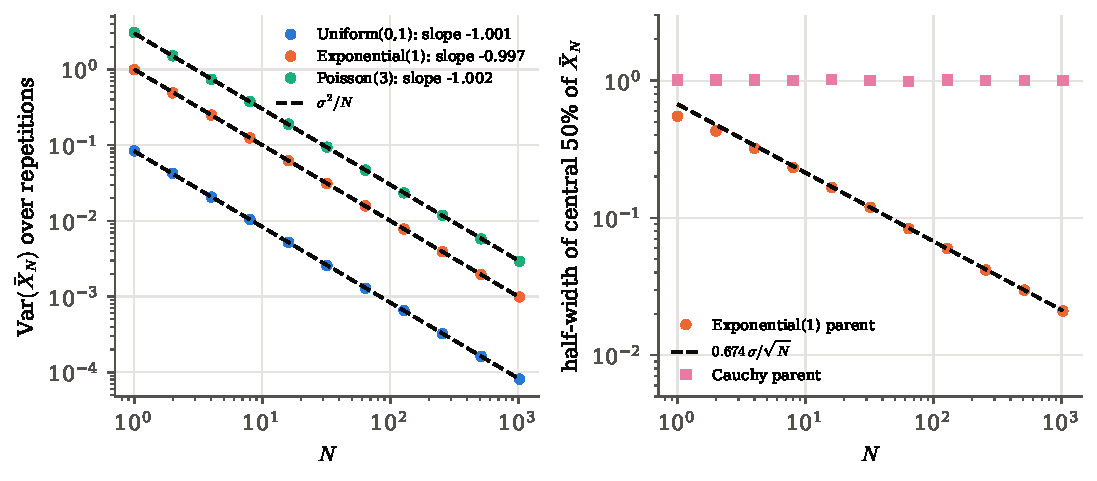
\includegraphics[width=12cm]{figures/ch03/var_mean_vs_N.pdf}
\caption{Left: the variance of the sample mean falls as $\sigma^2/N$ (dashed
lines) for three very different parents, a straight line of slope $-1$ on
log--log axes. Right: the width of the distribution of the mean falls as
$1/\sqrt N$ for exponential readings but stays flat for Cauchy readings,
where averaging a thousand values is no better than taking one.}
\label{3a:fig:var-mean-vs-N}
\end{figure}

\begin{figure}[htbp]
\centering
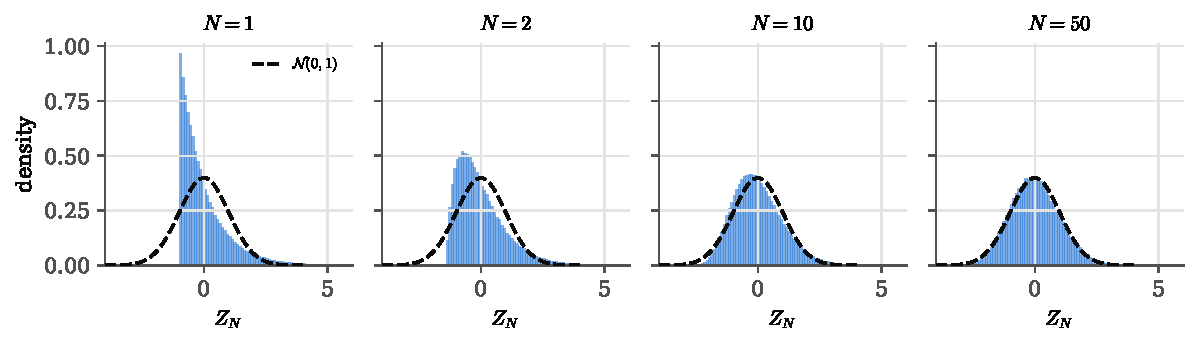
\includegraphics[width=12.5cm]{figures/ch03/clt_exponential.pdf}
\caption{The central limit theorem at work on exponential decay times.
Each panel is the histogram of the standardised mean $Z_N$ of $N$
exponential readings, over $200\,000$ repetitions, with the standard normal
curve dashed. At $N=1$ it is the exponential itself, cut off at $Z=-1$. By
$N=10$ it is close to Gaussian with a visible right skew, and by $N=50$ the
residual skewness $2/\sqrt{50}=0.28$ is hard to see.}
\label{3a:fig:clt-exponential}
\end{figure}

\paragraph{Asymptotically normal.}
An estimator is \newterm{asymptotically normal} if
$(\hat\theta_N-\theta)/\operatorname{se}\rightsquigarrow\Normal(0,1)$
\unpack{for large $N$ its sampling distribution is a Gaussian centred on the
truth with width equal to the standard error} \mainref{(6.8)}.

Most estimators we will meet are asymptotically normal: sample means by the
CLT, smooth functions of means by the delta method of
\cref{3a:sec:propagation}, and maximum-likelihood estimators by the argument
of the second half of \cref{ch:03}. That is why ``estimate $\pm$ standard
error'' means roughly a 68\% interval so often.

\begin{pitfall}[The CLT is about the mean, not about the data]
The CLT does not make the readings Gaussian, and it does not make every
statistic Gaussian. The histogram of individual muon decay times stays
exponential forever. It is the histogram of their \emph{average} that
becomes Gaussian. And it needs a finite variance: for Cauchy-like tails (a
resonance, a ratio of noisy quantities, \cref{3a:sec:ratio}) it fails
completely.
\end{pitfall}

\paragraph{What this bought us.}
Independent errors add like the steps of a random walk, so the scatter of a
mean is $\sigma/\sqrt N$ and its distribution approaches a Gaussian, with a
residual skewness that falls like $1/\sqrt N$. Correlations put a floor under
the error, and a parent without a variance defeats averaging altogether.

\paragraph{Verification and research.}
The log--log plot verifies $\sigma^2/N$ where we know $\sigma$. In a
Monte Carlo computation (\cref{ch:06}) we run the same check backwards: the
slope of the measured variance against $N$ tells us whether the samples are
really independent (slope $-1$) or correlated (a flatter slope, as for an
MCMC chain in \cref{ch:09}), and the plateau of a correlated run measures its
$N_{\mathrm{eff}}$.

\section{Estimating the scatter itself: the sample variance and its error}
\label{3a:sec:sample-variance}

The pendulum error bar $\sigma/\sqrt N$ contains the noise level $\sigma$,
which nobody told us. We must estimate it from the same ten readings. A
cosmologist faces the same task at every multipole: the angular power
spectrum $C_\ell$ \emph{is} a variance, the variance of the $2\ell+1$
spherical-harmonic coefficients $a_{\ell m}$, and estimating it from one sky
is estimating a variance from a finite sample. So is quoting the error bar
of a Monte Carlo average (\cref{ch:06}).

Two facts come out of this. The estimator of a variance that is right on
average divides by $N-1$, not by $N$. And that estimate has its own
uncertainty, the ``error on the error'', of which the cosmic-variance
formula is a special case.

\paragraph{Equipartition with the centre of mass removed.}
We cannot measure the spread of the readings about the unknown truth $\mu$,
only about their own average $\bar X$. Deviations from $\bar X$ are
systematically a little smaller than deviations from $\mu$, because the
average sits in the middle of the data by construction. How much smaller?
Think of $N$ particles of a gas,
each velocity component carrying energy $\tfrac12kT$ on average. If we
measure velocities relative to the centre of mass, one degree of freedom is
gone and the total relative kinetic energy is $(N-1)\tfrac12kT$. In the same
way, the $N$ deviations $X_i-\bar X$ sum to zero, only $N-1$ of them are
free, and each carries $\sigma^2$ on average.

\paragraph{What we want to know.}
\begin{enumerate}[label=\arabic*.]
  \item What is the average of $\sum_i(X_i-\bar X)^2$ over repetitions?
  \item What divisor makes the estimate of $\sigma^2$ right on average, and is
        that the best divisor?
  \item How much does the estimate of $\sigma^2$ itself scatter?
  \item What changes when the true mean is known, as for the $a_{\ell m}$
        of the CMB?
\end{enumerate}

\subsection{The $N-1$}
\label{3a:sec:n-minus-one}

Let $X_1,\dots,X_N$ be iid with mean $\mu$ and variance $\sigma^2$. The
question is the average, over repetitions, of the \newterm{sum of squared
deviations} $\mathrm{SS}=\sum_i(X_i-\bar X)^2$. We know the average of the
squared deviations from $\mu$; it is $\sigma^2$ each. So we first relate the
two sums. Write $X_i-\mu=(X_i-\bar X)+(\bar X-\mu)$ and square:
\begin{align}
  \sum_{i=1}^N(X_i-\mu)^2
  &\eqby{1} \sum_i(X_i-\bar X)^2+2(\bar X-\mu)\sum_i(X_i-\bar X)+N(\bar X-\mu)^2
     \nonumber\\
  &\eqby{2} \mathrm{SS}+N(\bar X-\mu)^2 .
  \label{3a:eq:ss-identity}
\end{align}
\begin{explain}
  \item Expand the square. The factor $\bar X-\mu$ does not depend on $i$ and
        comes out of the sum.
  \item $\sum_i(X_i-\bar X)=N\bar X-N\bar X=0$: deviations from the average sum
        to zero.
\end{explain}
This is again the parallel-axis theorem: spread about the truth equals
spread about the centre plus $N$ times the squared offset of the centre.
Now average over repetitions:
\begin{align}
  \E\,\mathrm{SS}
  &\eqby{1} \sum_{i=1}^N\E(X_i-\mu)^2-N\,\E(\bar X-\mu)^2
   \eqby{2} N\sigma^2-N\cdot\frac{\sigma^2}{N}
   = (N-1)\,\sigma^2 .
  \label{3a:eq:ess}
\end{align}
\begin{explain}
  \item Rearrange \eqref{3a:eq:ss-identity} and use linearity of expectation.
  \item $\E(X_i-\mu)^2=\sigma^2$ for each $i$, and $\E(\bar X-\mu)^2=\Var\bar X=\sigma^2/N$ from \eqref{3a:eq:var-mean}.
\end{explain}
The missing $\sigma^2$ is exactly the variance of the average: the data are
spread about $\bar X$, and $\bar X$ is itself off from $\mu$ by about
$\sigma/\sqrt N$.

\begin{workdef}[sample variance]
The \newterm{sample variance} is
\begin{equation}
  S^2=\frac{1}{N-1}\sum_{i=1}^N(X_i-\bar X)^2 ,
  \label{3a:eq:s2}
\end{equation}
and by \eqref{3a:eq:ess} it is unbiased, $\E S^2=\sigma^2$ \mainref{p.~52, Thm.~3.17}. The divisor
$N-1$ is the number of \newterm{degrees of freedom} \unpack{independent
directions left in the data after one direction was used to fix $\bar X$}.
If the true mean $\mu$ is \emph{known}, the estimator
$S_0^2=N^{-1}\sum_i(X_i-\mu)^2$ is unbiased with divisor $N$, since then
nothing was used up \srcref{Cowan}{(5.9)--(5.10)}.
\end{workdef}

\begin{figure}[htbp]
\centering
\begin{tikzpicture}[scale=1.0,font=\small]
  \draw[faint,->] (-0.3,0) -- (4.2,0) node[below] {$x_1$};
  \draw[faint,->] (0,-0.3) -- (0,3.8) node[left] {$x_2$};
  \draw[form,dashed] (-0.2,-0.2) -- (3.6,3.6);
  \node[formblue,anchor=west] at (3.6,3.6) {all readings equal};
  \coordinate (X) at (3.2,1.0);
  \coordinate (P) at (2.1,2.1);
  \coordinate (M) at (1.6,1.6);   %
  \draw[vec] (0,0) -- (X);
  \draw[fibre,very thick] (P) -- (X);
  \draw[bdry] (M) -- (P);
  \fill (X) circle (1.6pt);
  \fill[formblue] (P) circle (1.6pt);
  \fill[bdryred] (M) circle (1.6pt);
  \node[anchor=west] at (X) {$\ (x_1,x_2)$};
  \node[anchor=east,formblue] at (P) {$(\bar x,\bar x)\ $};
  \node[anchor=north west,bdryred] at (M) {$(\mu,\mu)$};
  \draw[thin] ($(P)!0.22cm!(X)$) -- ($(P)!0.22cm!(X)+(P)!0.22cm!(M)-(P)$) -- ($(P)!0.22cm!(M)$);
\end{tikzpicture}
\caption{Two readings as one point in the plane. The dashed diagonal holds
the data sets in which both readings are equal. The average $(\bar x,\bar x)$
is the foot of the perpendicular from the data point onto the diagonal. The
orange residual, of squared length $\mathrm{SS}$, lives in the one direction
perpendicular to the diagonal. The red segment is the offset of the average
from the truth. The right angle is the identity
\eqref{3a:eq:ss-identity}: distance$^2$ to the truth = orange$^2$ +
red$^2$.}
\label{3a:fig:projection}
\end{figure}

The geometry in \cref{3a:fig:projection} holds for any $N$. The data are a
vector in $\R^N$. The average is its projection on the line spanned by
$(1,1,\dots,1)$, and the residual vector $(X_i-\bar X)_i$ lives in the
$(N-1)$-dimensional subspace perpendicular to it. If the noise is isotropic
(independent, equal variance), each of those $N-1$ directions carries
variance $\sigma^2$, which is \eqref{3a:eq:ess} without algebra. For a
Gaussian parent we get the whole distribution, not just the average. Rotate
to a new orthonormal basis whose first axis is the diagonal. Independent
Gaussian noise of equal variance looks the same in every such basis, so the
new coordinates are again independent Gaussians of variance $\sigma^2$. The
first carries $\bar X$; the other $N-1$ carry the residual. So
$\mathrm{SS}/\sigma^2$ is a sum of $N-1$ squares of independent standard
normals, that is
\begin{equation}
  \frac{(N-1)S^2}{\sigma^2}\sim\chi^2_{N-1},
  \label{3a:eq:s2-chi2}
\end{equation}
independently of $\bar X$ (the $\chi^2$ distribution is in \cref{ch:02}).

\paragraph{Example: The pendulum's noise level.}
\label{3a:ex:pendulum-s}
For the ten readings of \cref{3a:sec:sampling}, $\bar x=9.815$ and the
deviations are $-0.025,0.015,0.045,-0.015,-0.045,0.025,-0.005,-0.035,0.035,0.005$.
Their squares sum to
$2(0.025^2+0.015^2+0.045^2+0.035^2+0.005^2)=2\times0.004125=0.00825$. Hence
\begin{align*}
  s^2 &\eqby{1} \frac{0.00825}{9}=9.17\times10^{-4},\qquad s=0.0303,\qquad
  \widehat{\operatorname{se}}(\bar x) \eqby{2} \frac{s}{\sqrt{10}}=0.0096\ \mathrm{m\,s^{-2}} .
\end{align*}
\begin{explain}
  \item Divide the sum of squared deviations by $N-1=9$.
  \item The estimated standard error of the mean replaces $\sigma$ by $s$ in \eqref{3a:eq:var-mean}.
\end{explain}
The result is $g=9.815\pm0.010\,\mathrm{m\,s^{-2}}$. How much should we trust
the ``$\pm0.010$''? That is the question of \cref{3a:sec:var-of-var}.

\paragraph{Example: $S^2$ is consistent.}
\label{3a:ex:s2-consistent}
Expanding the square in \eqref{3a:eq:s2},
$\sum_i(X_i-\bar X)^2=\sum_iX_i^2-N\bar X^2$, so
\begin{align*}
  S^2
  &\eqby{1} \frac{N}{N-1}\Bigl[\frac1N\sum_{i=1}^NX_i^2-\bar X^2\Bigr]
   \;\xrightarrow{\;P\;}\; 1\cdot\bigl[\E X^2-\mu^2\bigr] \eqby{2} \sigma^2 .
\end{align*}
\begin{explain}
  \item Factor out $N/(N-1)$. Inside the bracket, the first term is the mean of
        the iid variables $X_i^2$, which tends in probability to $\E X^2$ by the
        WLLN. $\bar X\xrightarrow{P}\mu$ and squaring is continuous, so
        $\bar X^2\xrightarrow{P}\mu^2$. Sums and products of sequences that
        converge in probability converge to the sums and products of the
        limits, and $N/(N-1)\to1$.
  \item $\E X^2-\mu^2=\sigma^2$.
\end{explain}
\srcref{CasellaBerger}{Ex.~5.5.3}; \mainref{Exercise~5.1}. The same argument
applied with the continuous map $\sqrt{\cdot}$ gives $S\xrightarrow{P}\sigma$.

\begin{pitfall}[$S$ is a biased estimator of $\sigma$]
Unbiasedness does not survive nonlinear maps. Because
$\Var S=\E S^2-(\E S)^2\ge0$, we have $(\E S)^2\le\E S^2=\sigma^2$, so
$\E S\le\sigma$, with equality only if $S$ never fluctuates (this is
Jensen's inequality for the concave square root). For Gaussian data,
$\E S=c_4(N)\,\sigma$ with
$c_4(N)=\sqrt{2/(N-1)}\;\Gamma(N/2)/\Gamma\bigl((N-1)/2\bigr)$, which follows
from the mean of the square root of a $\chi^2_{N-1}$ variable. For $N=5$,
$c_4=\ThreeACfourFive$; the simulation gives $\E S/\sigma=\ThreeAMeanSFive$.
$S$ is biased for every finite $N$ but consistent
\srcref{CasellaBerger}{Ex.~5.5.5}.
\end{pitfall}

\subsection{Is $N-1$ the best divisor?}
\label{3a:sec:best-divisor}

Unbiased is not the same as best (\cref{3a:sec:bias-variance}). For
Gaussian data we can compute the MSE of $W_d=\mathrm{SS}/d$ for any divisor
$d$, because by \eqref{3a:eq:s2-chi2} $\mathrm{SS}=\sigma^2\chi^2_{N-1}$ and
a $\chi^2_\nu$ variable has mean $\nu$ and variance $2\nu$.

\paragraph{Example: The divisor that minimises the MSE.}
\label{3a:ex:divisor}
\begin{align*}
  \operatorname{MSE}(W_d)
  &\eqby{1} \Bigl(\frac{(N-1)\sigma^2}{d}-\sigma^2\Bigr)^2+\frac{2(N-1)\sigma^4}{d^2}
   \eqby{2} \sigma^4\Bigl[\bigl((N-1)u-1\bigr)^2+2(N-1)u^2\Bigr],\quad u=\frac1d .
\end{align*}
\begin{explain}
  \item Squared bias plus variance \eqref{3a:eq:mse-decomp}, with $\E W_d=(N-1)\sigma^2/d$ and $\Var W_d=2(N-1)\sigma^4/d^2$.
  \item Factor out $\sigma^4$ and write $u=1/d$.
\end{explain}
Setting the $u$-derivative to zero,
$2(N-1)\bigl[(N-1)u-1\bigr]+4(N-1)u=0$, i.e.\ $(N+1)u=1$. The minimum is at
$d=N+1$. For $N=10$ the three candidates give
\[
  d=N-1:\ \tfrac29=0.222,\qquad d=N:\ 0.01+0.18=0.190,\qquad
  d=N+1:\ \tfrac{4}{121}+\tfrac{18}{121}=0.182
\]
(in units of $\sigma^4$). The simulation gives $\ThreeAMseNmOneTen$,
$\ThreeAMseNTen$ and $\ThreeAMseNpOneTen$.

So the unbiased $S^2$ does not have the smallest MSE. Even $d=N$ beats it
\srcref{CasellaBerger}{Exs.~7.3.3--7.3.4}: the biased maximum-likelihood
estimator $\hat\sigma^2=\mathrm{SS}/N$ has MSE $(2N-1)\sigma^4/N^2$, smaller
than the $2\sigma^4/(N-1)$ of $S^2$. A larger divisor shrinks the estimate
towards zero, trading a small downward bias for a reduction in variance.

Why, then, do we usually quote $S^2$? For two reasons. First, estimates are
often \emph{averaged} later, and when they are, biases add up while scatter
averages away; an unbiased estimate is then what we want. Second, the
optimal divisor depends on the parent: $N+1$ is special to Gaussian data.

\subsection{The variance of the variance}
\label{3a:sec:var-of-var}

How much does $S^2$ scatter? The answer involves the fourth central moment
$\mu_4=\E(X-\mu)^4$. Without loss of generality set $\mu=0$ (shifting every
reading by a constant changes neither $S^2$ nor the central moments). Using
$\sum_i(X_i-\bar X)^2=\sum_iX_i^2-\frac1N\sum_{i,j}X_iX_j$, split $S^2$ into
a ``diagonal'' and an ``off-diagonal'' part:
\begin{equation}
  S^2=\underbrace{\frac1N\sum_{i}X_i^2}_{A}\;-\;
  \underbrace{\frac{1}{N(N-1)}\sum_{i\neq j}X_iX_j}_{B} .
  \label{3a:eq:s2-split}
\end{equation}
(The coefficient of $X_i^2$ is $\frac{1}{N-1}(1-\frac1N)=\frac1N$, and that of
$X_iX_j$, $i\neq j$, is $\frac{1}{N-1}\cdot\frac1N$.) The variance of a
difference is $\Var(A-B)=\Var A+\Var B-2\Cov(A,B)$, so we need three pieces.
\begin{align}
  \Var A
  &\eqby{1} \frac{1}{N^2}\,N\,\Var(X^2)
   \eqby{2} \frac{\mu_4-\sigma^4}{N}, \label{3a:eq:varA}\\
  \E B^2
  &\eqby{3} \frac{1}{N^2(N-1)^2}\sum_{i\neq j}\sum_{k\neq l}\E[X_iX_jX_kX_l]
   \eqby{4} \frac{2N(N-1)\sigma^4}{N^2(N-1)^2}
   = \frac{2\sigma^4}{N(N-1)}, \label{3a:eq:varB}\\
  \Cov(A,B)
  &\eqby{5} \frac{1}{N^2(N-1)}\sum_k\sum_{i\neq j}\E[X_k^2X_iX_j]
   \eqby{6} 0 . \label{3a:eq:covAB}
\end{align}
\begin{explain}
  \item The $X_i^2$ are independent, so the variance of their sum is the sum of their variances.
  \item $\Var(X^2)=\E X^4-(\E X^2)^2=\mu_4-\sigma^4$ (recall $\mu=0$).
  \item $\E B=0$ because each term has $\E X_iX_j=\E X_i\,\E X_j=0$. So
        $\Var B=\E B^2$, which is the double sum over pairs of pairs.
  \item A product $X_iX_jX_kX_l$ with $i\neq j$ has zero mean unless every index
        appears at least twice, which forces $\{k,l\}=\{i,j\}$. There are two
        such choices, $(k,l)=(i,j)$ or $(j,i)$, each giving
        $\E X_i^2X_j^2=\sigma^4$. There are $N(N-1)$ ordered pairs $(i,j)$.
  \item $\E B=0$, so $\Cov(A,B)=\E[AB]$. Multiply out the two sums.
  \item Since $i\neq j$, at least one of $i,j$ differs from $k$ and from the
        other index, so it appears once and its factor $\E X=0$ kills the term.
\end{explain}
Putting the pieces together,
\begin{align}
  \Var S^2
  &\eqby{1} \Var A+\Var B-2\Cov(A,B)
   \eqby{2} \frac{\mu_4-\sigma^4}{N}+\frac{2\sigma^4}{N(N-1)} \nonumber\\
  &\eqby{3} \frac1N\Bigl[\mu_4-\frac{N-3}{N-1}\,\sigma^4\Bigr] .
  \label{3a:eq:var-s2}
\end{align}
\begin{explain}
  \item Variance of a difference.
  \item Insert \eqref{3a:eq:varA}--\eqref{3a:eq:covAB}.
  \item $-\sigma^4+\frac{2\sigma^4}{N-1}=-\sigma^4\,\frac{N-1-2}{N-1}$.
\end{explain}
This is \srcref{Cowan}{(5.14)}. For a Gaussian parent, $\mu_4=3\sigma^4$ (from
Isserlis' theorem, or by direct integration: $\E Z^4=3$ for a standard
normal), and
\begin{equation}
  \Var S^2\big|_{\text{Gauss}}
  =\frac{\sigma^4}{N}\,\frac{3(N-1)-(N-3)}{N-1}=\frac{2\sigma^4}{N-1},
  \label{3a:eq:var-s2-gauss}
\end{equation}
in agreement with $\Var\chi^2_{N-1}=2(N-1)$ in \eqref{3a:eq:s2-chi2}.

\paragraph{The error on the error.}
For Gaussian data the relative error of $S^2$ is $\sqrt{2/(N-1)}$, and that
of $S$ is half as large (a relative error halves under a square root; this
is the propagation rule of \cref{3a:sec:propagation}):
\begin{equation}
  \frac{\operatorname{se}(S)}{\sigma}\approx\frac{1}{\sqrt{2(N-1)}} .
  \label{3a:eq:error-on-error}
\end{equation}
With ten readings an error bar is itself uncertain by about 24\%. With a
hundred, by 7\%. Quoting an error bar to three significant figures from ten
points is meaningless.

For a heavy-tailed parent the variance of $S^2$ is larger, because $\mu_4$
weights the tails heavily. An exponential parent of mean $\tau$ has
$\sigma=\tau$ and $\mu_4=9\tau^4=9\sigma^4$, three times the Gaussian value.
To quote the
uncertainty of $S^2$ from data, replace $\mu_4$ by the sample moment
$m_4=\frac1N\sum_i(X_i-\bar X)^4$ \srcref{Cowan}{(5.15)}.

\paragraph{Example: Cosmic variance.}
\label{3a:ex:cosmic-variance}
In a statistically isotropic Gaussian sky, the $2\ell+1$ coefficients
$a_{\ell m}$ at multipole $\ell$ behave (for this count) like $2\ell+1$
independent real Gaussian variables of mean zero and variance $C_\ell$
(the precise complex bookkeeping is in \cref{ch:07}). The natural estimator
$\Chat=\frac{1}{2\ell+1}\sum_m|a_{\ell m}|^2$ is the known-mean estimator
$S_0^2$ with $N=2\ell+1$. With known mean zero, $\sum_ma_{\ell m}^2/C_\ell$
is a sum of $2\ell+1$ squared standard normals, i.e.\ $\chi^2_{2\ell+1}$, so
\begin{align*}
  \E\Chat &\eqby{1} \frac{C_\ell}{2\ell+1}\,(2\ell+1)=C_\ell,\qquad
  \Var\Chat \eqby{2} \frac{C_\ell^2}{(2\ell+1)^2}\cdot2(2\ell+1)=\frac{2C_\ell^2}{2\ell+1}.
\end{align*}
\begin{explain}
  \item A $\chi^2_\nu$ variable has mean $\nu$.
  \item It has variance $2\nu$, and $\Var(cU)=c^2\Var U$ with $c=C_\ell/(2\ell+1)$.
\end{explain}
This is \newterm{cosmic variance}: the relative error
$\sqrt{2/(2\ell+1)}$ is 63\% at the quadrupole $\ell=2$ and cannot be reduced,
because we have only one sky. It is the known-mean version of
\eqref{3a:eq:var-s2-gauss}, with $N$ in place of $N-1$ because no degree of
freedom is spent on estimating a mean.

\subsection{Seeing it in Python}
\label{3a:sec:var-python}

\pyfile[firstline=29,lastline=39]{code/ch03/04_sample_variance.py}{The two divisors and the scatter of $S^2$}

Each row of \pyname{x} is one experiment of $N$ standard normal readings
($\sigma=1$). The script forms $\mathrm{SS}$ row by row, divides by $N$ and
by $N-1$, and averages over the $M=100\,000$ rows. It also records the
variance of $S^2$ across rows and the MSE of the three divisors. The last
three lines repeat the variance measurement for an exponential parent. For
$N=5$ the average of $\mathrm{SS}/N$ is $\ThreeAVbiasFive$ (derived:
$4/5=0.8$) and of $\mathrm{SS}/(N-1)$ is $\ThreeAVunbFive$ (derived: $1$).
At $N=10$, $\Var S^2=\ThreeAVarSGaussTen$ for Gaussian readings (derived
$\ThreeAVarSGaussTenTh$) and $\ThreeAVarSExpTen$ for exponential ones
(derived from \eqref{3a:eq:var-s2} with $\mu_4=9$: $\ThreeAVarSExpTenTh$).

\begin{figure}[htbp]
\centering
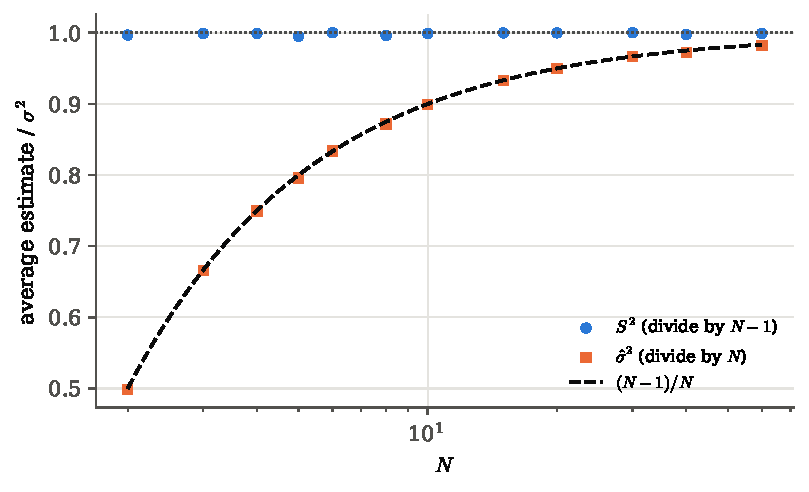
\includegraphics[width=10.5cm]{figures/ch03/variance_bias.pdf}
\caption{Average of two variance estimators over $100\,000$ Gaussian
experiments, as a function of the number of readings. Dividing by $N-1$ is
right on average at every $N$. Dividing by $N$ falls short by the factor
$(N-1)/N$ (dashed), badly for $N=2$ and negligibly beyond a few tens.}
\label{3a:fig:variance-bias}
\end{figure}

\begin{figure}[htbp]
\centering
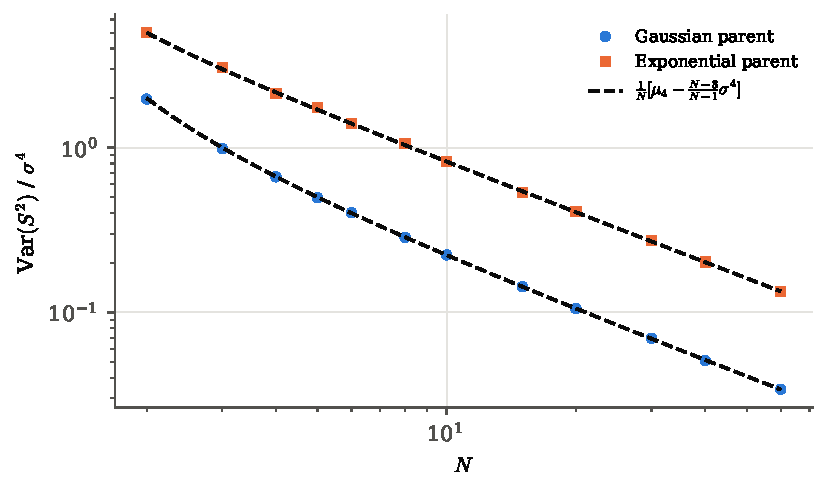
\includegraphics[width=10.5cm]{figures/ch03/variance_of_variance.pdf}
\caption{Scatter of the sample variance over repetitions. Both parents follow
the derived formula \eqref{3a:eq:var-s2} (dashed), falling roughly as $1/N$.
The exponential parent, with its long tail, has a variance of the variance
about four times larger than the Gaussian at the same $N$.}
\label{3a:fig:variance-of-variance}
\end{figure}

\paragraph{What this bought us.}
Divide by $N-1$ because one degree of freedom went into $\bar X$. The
resulting $S^2$ is unbiased but has its own scatter,
$\Var S^2=\frac1N[\mu_4-\frac{N-3}{N-1}\sigma^4]$, which for Gaussian data
means a relative error of $1/\sqrt{2(N-1)}$ on $S$. With a known mean the
divisor is $N$, and the Gaussian scatter $2\sigma^4/N$ is cosmic variance.

\paragraph{Verification and research.}
Here the simulation verifies \eqref{3a:eq:var-s2}. The formula is needed
later as an instrument: the error bar of any Monte Carlo estimate of a
variance, and hence of every simulated covariance matrix
(\cref{3a:sec:covariance}), is set by it. For a masked sky the $a_{\ell m}$
are no longer independent, the effective number of modes drops below
$2\ell+1$, often to roughly $\fsky(2\ell+1)$, and the true variance of the
power spectrum estimate is found by simulation (\cref{ch:08}).

\section{Estimating covariance and correlation matrices, and how noisy they are}
\label{3a:sec:covariance}

A CMB or galaxy-survey analysis compresses a map into $p=20$ band powers and
compares them with theory through a $\chi^2=(\data-\bm m)\T\Cmat^{-1}(\data-\bm m)$.
The covariance matrix $\Cmat$ of the band powers has no formula once masks
and noise enter, so we run $n$ simulations and estimate it from the scatter
of the simulated band powers. Supercomputer time limits us to, say, $n=50$.
The resulting matrix shows correlations between bins that are not there,
and its inverse is too large. In the same way a detector with twenty
readout channels shows ``cross-talk'' between channels that is just noise.

The sample variance, extended to a matrix, tells us how noisy each element
is, and so how large the false correlations can be. A change of variable
gives a reliable error bar for a real correlation. And a single factor
removes the bias of the inverse.

\paragraph{A tilted cloud, seen through few points.}
A correlation coefficient measures the tilt of a cloud of points in a
scatter plot. With a thousand points the tilt is obvious. With ten points
drawn from a perfectly round cloud, the ten happen to line up a little by
chance, and a tilt appears. A $20\times20$ correlation matrix has $190$
tilts to get wrong, so some of them will be large by chance. It is the same
reason why a few stars in the sky seem to form constellations.

\paragraph{The questions, in words.}
\begin{enumerate}[label=\arabic*.]
  \item How do we estimate, without bias, the covariance of two quantities
        from paired readings?
  \item If two quantities are truly unrelated, how large a sample
        correlation can chance produce?
  \item For a real correlation, what is the sampling distribution of its
        estimate, and how do we put an error bar on it?
  \item What happens when we invert a noisy covariance matrix?
\end{enumerate}

\subsection{The sample covariance matrix}
\label{3a:sec:sample-cov}

Recall from \cref{ch:02} the covariance
$\Sigma_{ab}=\Cov(X_a,X_b)=\E[(X_a-\mu_a)(X_b-\mu_b)]$ of two components of
a random vector $\bm X=(X_1,\dots,X_p)$, and the correlation
$\rho_{ab}=\Sigma_{ab}/\sqrt{\Sigma_{aa}\Sigma_{bb}}$, which lies in $[-1,1]$.

\begin{workdef}[sample covariance and correlation]
Given $n$ independent readings $\bm x_1,\dots,\bm x_n$ of a $p$-component
vector \unpack{each $\bm x_j$ is one simulation, or one event, giving all
$p$ numbers at once}, with average $\bar{\bm x}=n^{-1}\sum_j\bm x_j$, the
\newterm{sample covariance matrix} is
\begin{equation}
  \hat\Cmat=\frac{1}{n-1}\sum_{j=1}^n(\bm x_j-\bar{\bm x})(\bm x_j-\bar{\bm x})\T,
  \qquad
  \hat C_{ab}=\frac{1}{n-1}\sum_{j=1}^n(x_{aj}-\bar x_a)(x_{bj}-\bar x_b),
  \label{3a:eq:sample-cov}
\end{equation}
and the \newterm{sample correlation} is
\begin{equation}
  r_{ab}=\frac{\hat C_{ab}}{\sqrt{\hat C_{aa}\hat C_{bb}}}
  =\frac{\sum_j(x_{aj}-\bar x_a)(x_{bj}-\bar x_b)}
        {\sqrt{\sum_j(x_{aj}-\bar x_a)^2\,\sum_j(x_{bj}-\bar x_b)^2}} .
  \label{3a:eq:sample-corr}
\end{equation}
\end{workdef}

In \eqref{3a:eq:sample-corr} the factors $1/(n-1)$ cancel between numerator
and denominator, which gives the second form; by the Cauchy--Schwarz
inequality it always satisfies $|r|\le1$. The printed formula
\mainref{(14.6)} drops the $1/(n-1)$ from the numerator only, which would
let $|r|$ exceed $1$. The form above is the correct one and agrees with
\srcref{Cowan}{(5.12)}.

The diagonal of $\hat\Cmat$ holds the sample variances of
\cref{3a:sec:sample-variance}. The off-diagonal elements are unbiased by the
same argument. Write $\bm y_j=\bm x_j-\bm\mu$, so that
$\bm x_j-\bar{\bm x}=\bm y_j-\bar{\bm y}$, and use
$\sum_j(\bm y_j-\bar{\bm y})(\bm y_j-\bar{\bm y})\T=\sum_j\bm y_j\bm y_j\T-n\,\bar{\bm y}\bar{\bm y}\T$
(the matrix version of \eqref{3a:eq:ss-identity}):
\begin{align}
  \E\Bigl[\sum_{j}(\bm x_j-\bar{\bm x})(\bm x_j-\bar{\bm x})\T\Bigr]
  &\eqby{1} \sum_j\E[\bm y_j\bm y_j\T]-n\,\E[\bar{\bm y}\bar{\bm y}\T]
   \eqby{2} n\bm\Sigma-n\cdot\frac{\bm\Sigma}{n}
   = (n-1)\,\bm\Sigma .
  \label{3a:eq:cov-unbiased}
\end{align}
\begin{explain}
  \item Linearity of expectation applied element by element.
  \item $\E[\bm y_j\bm y_j\T]=\bm\Sigma$ by definition. For the mean,
        $\E[\bar y_a\bar y_b]=n^{-2}\sum_{j,k}\E[y_{aj}y_{bk}]=n^{-2}\cdot n\,\Sigma_{ab}$,
        because readings $j\neq k$ are independent with zero mean.
\end{explain}
So $\E\hat\Cmat=\bm\Sigma$ \mainref{p.~233, (14.4)}. A handy form for
computing is $\hat C_{ab}=\frac{n}{n-1}\bigl(\overline{x_ax_b}-\bar x_a\bar x_b\bigr)$,
where the bar means the average over readings \srcref{Cowan}{(5.11)}.

\paragraph{Example: A $2\times2$ covariance by hand.}
\label{3a:ex:cov-hand}
Four paired readings $(x,y)=(1,2),(2,1),(3,4),(4,3)$. Both averages are
$2.5$. The deviations are $\delta x=(-1.5,-0.5,0.5,1.5)$ and
$\delta y=(-0.5,-1.5,1.5,0.5)$. Then
\begin{align*}
  \hat C_{xx} &\eqby{1} \tfrac13(2.25+0.25+0.25+2.25)=\tfrac53,\qquad
  \hat C_{yy}\eqby{2}\tfrac53,\\
  \hat C_{xy} &\eqby{3} \tfrac13(0.75+0.75+0.75+0.75)=1,\qquad
  r \eqby{4} \frac{1}{\sqrt{(5/3)(5/3)}}=0.6 .
\end{align*}
\begin{explain}
  \item Squares of the $x$ deviations, divided by $n-1=3$.
  \item The $y$ deviations are a permutation of the $x$ ones, so the same sum.
  \item Products $(-1.5)(-0.5)$, $(-0.5)(-1.5)$, $(0.5)(1.5)$, $(1.5)(0.5)$, each $0.75$.
  \item Definition \eqref{3a:eq:sample-corr}.
\end{explain}
Four points already give a respectable-looking $r=0.6$. Is it real? To
answer, we need to know how large $r$ gets when there is no correlation at
all.

\subsection{Correlations from pure noise}
\label{3a:sec:spurious}

\begin{figure}[htbp]
\centering
\begin{tikzpicture}[font=\small]
  \coordinate (O) at (0,0);
  \coordinate (A) at (3.6,0.4);
  \coordinate (B) at (2.2,2.4);
  \draw[vec] (O) -- (A);
  \draw[vec,formblue] (O) -- (B);
  \node[anchor=west] at (A) {$\ \bm a=(x_{aj}-\bar x_a)_j$};
  \node[anchor=south,formblue] at (B) {$\bm b=(x_{bj}-\bar x_b)_j$};
  \pic[draw,angle radius=9mm,"$\varphi$",angle eccentricity=1.35] {angle=A--O--B};
  \draw[faint,dashed] (B) -- ($(O)!(B)!(A)$);
  \node[anchor=north east,align=right,font=\footnotesize] at (-0.2,-0.2)
       {$r=\cos\varphi=\dfrac{\bm a\cdot\bm b}{|\bm a|\,|\bm b|}$};
\end{tikzpicture}
\caption{The sample correlation as an angle. The deviations of the $n$
readings of each quantity form two vectors in $\R^n$, both perpendicular to
$(1,\dots,1)$ and so living in an $(n-1)$-dimensional space. The sample
correlation is the cosine of the angle between them. Uncorrelated noise
points $\bm b$ in a random direction relative to $\bm a$.}
\label{3a:fig:corr-angle}
\end{figure}

Formula \eqref{3a:eq:sample-corr} is a dot product divided by two lengths,
so it is the cosine of the angle between the two deviation vectors in
\cref{3a:fig:corr-angle}. This picture gives the spread of $r$ for unrelated
quantities without any integrals.

\paragraph{Example: The scatter of $r$ when $\rho=0$.}
\label{3a:ex:r-null}
Let the two quantities be independent Gaussians. As in
\cref{3a:fig:projection}, the deviation vectors live in the
$(m=n-1)$-dimensional subspace perpendicular to $(1,\dots,1)$, and in it the
Gaussian noise vector $\bm b$ is isotropic: its direction $\bm u=\bm b/|\bm b|$ is
uniformly distributed on the unit sphere, independently of $\bm a$. Rotate
coordinates so that $\bm a$ points along the first axis. Then $r=u_1$ and
\begin{align*}
  \E r \eqby{1} 0,\qquad
  \E r^2=\E u_1^2
  &\eqby{2} \frac1m\sum_{k=1}^m\E u_k^2
   \eqby{3} \frac1m\,\E\Bigl[\sum_{k=1}^mu_k^2\Bigr]
   \eqby{4} \frac1m=\frac{1}{n-1} .
\end{align*}
\begin{explain}
  \item $\bm u$ and $-\bm u$ are equally likely.
  \item By symmetry every component of a uniform unit vector has the same
        mean square.
  \item Linearity of expectation.
  \item A unit vector has $\sum_ku_k^2=1$ exactly.
\end{explain}
So for unrelated quantities $r$ scatters about zero with standard deviation
$1/\sqrt{n-1}$, and for large $n$ it is close to Gaussian. With $n=4$ as in
\cref{3a:ex:cov-hand}, $1/\sqrt3=0.58$: our $r=0.6$ is one standard deviation
from zero and means nothing.

\begin{keyidea}[Spurious correlations]
If $p$ quantities are truly independent, each of the $p(p-1)/2$ off-diagonal
sample correlations scatters about zero with standard deviation about
$1/\sqrt{n-1}$. Among many pairs, roughly 5\% exceed $1.96/\sqrt{n-1}$ in
magnitude by chance alone.
\end{keyidea}

With $p=20$ and $n=50$ there are $\ThreeANpairs$ pairs. The prediction is a
spread of $1/\sqrt{49}=\ThreeASpurSdTh$ and about ten pairs beyond
$|r|=0.28$. The simulation (\cref{3a:fig:spurious}) gives a spread of
$\ThreeASpurSd$ in one realisation and a largest $|r|$ of $\ThreeASpurMax$.
Searching a large matrix for the most correlated pair and then quoting its
significance as if it were the only pair examined is the \emph{look-elsewhere
effect} of \cref{ch:04}.

\begin{figure}[htbp]
\centering
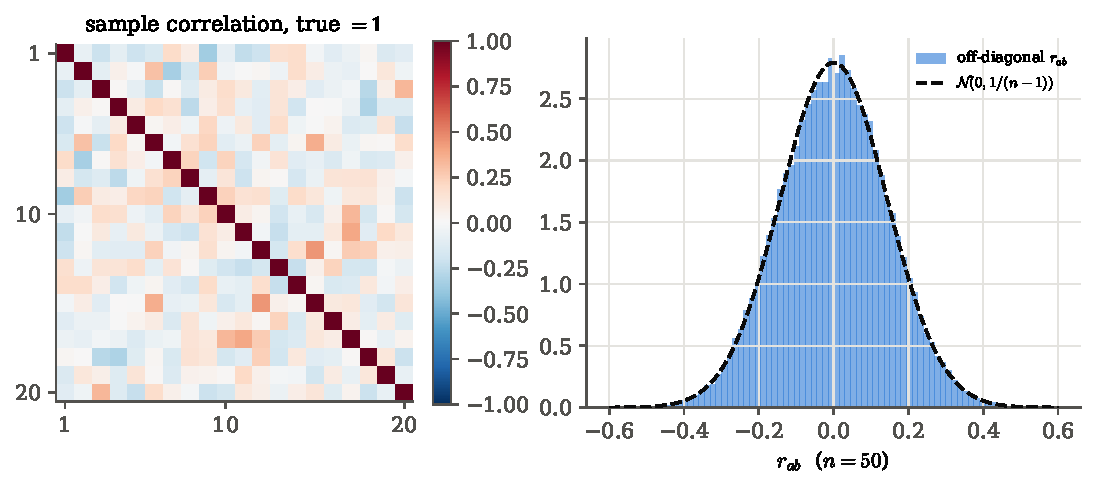
\includegraphics[width=12cm]{figures/ch03/spurious_correlations.pdf}
\caption{Left: the sample correlation matrix of twenty independent quantities
from fifty readings. The true matrix is the identity. Every coloured
off-diagonal square is noise, and some reach $\pm0.4$. Right: the
off-diagonal elements from 400 such matrices, with the Gaussian of standard
deviation $1/\sqrt{n-1}$ (dashed).}
\label{3a:fig:spurious}
\end{figure}

\subsection{A real correlation, its error bar, and Fisher's $z$}
\label{3a:sec:fisher-z}

For a bivariate Gaussian with correlation $\rho\neq0$, the sample correlation
is biased and skewed, with, to leading order in $1/n$
\srcref{Cowan}{(5.16)--(5.17)},
\begin{equation}
  \E r\approx\rho-\frac{\rho(1-\rho^2)}{2n},\qquad
  \Var r\approx\frac{(1-\rho^2)^2}{n}.
  \label{3a:eq:r-moments}
\end{equation}
The variance shrinks as $|\rho|\to1$, because $r$ cannot exceed $1$: the
sampling distribution is squashed against the wall and develops a long tail
towards zero. An error bar $r\pm\sqrt{\Var r}$ is then misleading, since it
depends on the unknown $\rho$ and may poke above $1$.

Fisher's remedy is a change of variable that makes the width independent of
$\rho$. We look for $z=h(r)$ with $\Var z$ constant. To first order in the
fluctuation (the propagation rule derived in \cref{3a:sec:propagation}),
$\Var h(r)\approx h'(\rho)^2\Var r$, so we need
$h'(\rho)\propto1/(1-\rho^2)$:
\begin{align}
  h(\rho)
  &\eqby{1} \int_0^\rho\frac{\dd s}{1-s^2}
   \eqby{2} \frac12\int_0^\rho\Bigl(\frac{1}{1+s}+\frac{1}{1-s}\Bigr)\dd s
   \eqby{3} \frac12\ln\frac{1+\rho}{1-\rho}=\operatorname{artanh}\rho .
  \label{3a:eq:fisher-z}
\end{align}
\begin{explain}
  \item Choose the integration constant so that $h(0)=0$.
  \item Partial fractions: $\frac{1}{1-s^2}=\frac12\bigl(\frac{1}{1+s}+\frac{1}{1-s}\bigr)$.
  \item Integrate: $\ln(1+s)-\ln(1-s)$, evaluated from $0$ to $\rho$.
\end{explain}
Then $\Var z\approx(1-\rho^2)^{-2}(1-\rho^2)^2/n=1/n$. A finer calculation
replaces $n$ by $n-3$, and $z$ is very nearly Gaussian even for small $n$:
\begin{equation}
  z=\operatorname{artanh}r\approx\Normal\Bigl(\operatorname{artanh}\rho,\ \frac{1}{n-3}\Bigr).
  \label{3a:eq:fisher-z-dist}
\end{equation}
The inverse map is $\rho=\tanh z=(e^{2z}-1)/(e^{2z}+1)$. The map stretches
the region near $\pm1$, which pulls the squashed tail back into a
symmetric shape.

\paragraph{Example: An interval for a correlation.}
\label{3a:ex:fisher-interval}
We observe $r=0.6$ from $n=20$ pairs. A 95\% interval is built in $z$ and
mapped back \mainref{p.~234}:
\begin{align*}
  \hat z &\eqby{1} \operatorname{artanh}0.6=\tfrac12\ln4=0.693,\qquad
  \frac{1.96}{\sqrt{n-3}} \eqby{2} \frac{1.96}{\sqrt{17}}=0.475,\\
  (a,b) &\eqby{3} (0.218,\ 1.169),\qquad
  (\tanh a,\tanh b) \eqby{4} (0.214,\ 0.824).
\end{align*}
\begin{explain}
  \item $\frac12\ln\frac{1.6}{0.4}=\frac12\ln4$.
  \item The standard deviation of $z$ from \eqref{3a:eq:fisher-z-dist}, times $1.96$.
  \item $\hat z\mp0.475$.
  \item Map each end back with $\tanh$, which is increasing, so the order is kept.
\end{explain}
The interval $(0.21,0.82)$ is asymmetric about $0.6$, longer on the side
away from the wall at $1$, exactly as the skewed sampling distribution
demands.

\pyfile[firstline=50,lastline=56]{code/ch03/05_covariance_noise.py}{Simulating the sample correlation for $\rho=0.6$, $n=20$}

The script makes correlated pairs by multiplying independent standard
normals by the Cholesky factor $L$ of the target $2\times2$ correlation
matrix ($LL\T$ equals that matrix, so $L\bm\epsilon$ has exactly that
covariance, \cref{ch:02}). It removes the mean of each column within every
experiment and applies \eqref{3a:eq:sample-corr} row by row. Over
$100\,000$ experiments the mean of $r$ is $\ThreeARMean$ (from
\eqref{3a:eq:r-moments}: $\ThreeARMeanTh$), its spread $\ThreeARSd$ (leading
order: $\ThreeARSdTh$, an underestimate at this small $n$) and its skewness
$\ThreeARSkew$. For $z$, the spread is $\ThreeAZSd$ against
$1/\sqrt{17}=\ThreeAZSdTh$, and the skewness $\ThreeAZSkew$: Fisher's
transformation has removed it.

\begin{figure}[htbp]
\centering
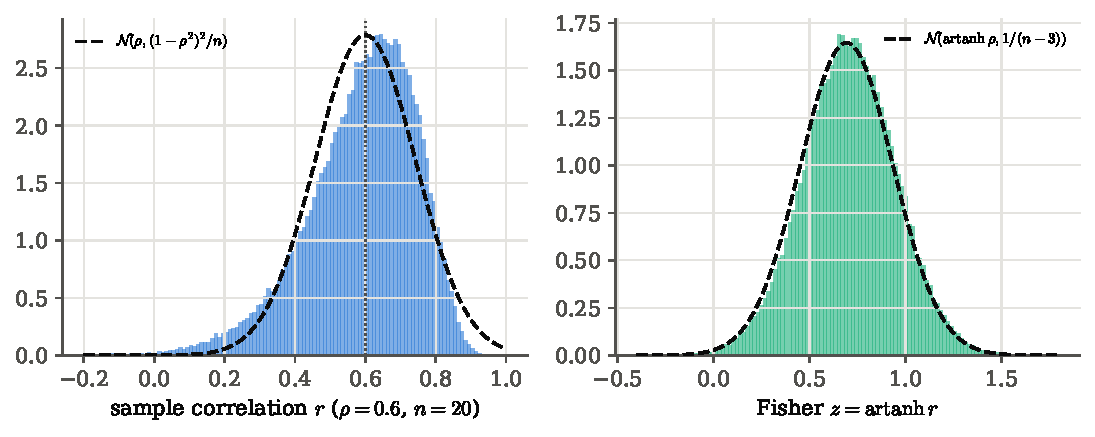
\includegraphics[width=12cm]{figures/ch03/corr_fisher_z.pdf}
\caption{Left: the sample correlation from twenty pairs with true
correlation $0.6$ (dotted). It is skewed, with a long tail towards zero, and
the leading-order Gaussian (dashed) is too narrow on that side. Right: the
same experiments after Fisher's transformation $z=\operatorname{artanh}r$.
The histogram now sits on a symmetric Gaussian of width $1/\sqrt{n-3}$.}
\label{3a:fig:fisher-z}
\end{figure}

\subsection{How noisy is every element, and what inversion does}
\label{3a:sec:cov-noise}

For Gaussian readings there is a clean formula for the scatter of each
element of $\hat\Cmat$. The rotation argument of
\cref{3a:sec:n-minus-one}, applied to each component, turns the $n$ centred
readings into $n-1$ independent vectors $\bm z_k\sim\Normal(\bm0,\bm\Sigma)$,
with $(n-1)\hat\Cmat=\sum_{k=1}^{n-1}\bm z_k\bm z_k\T$. We need one fact
about Gaussian fourth moments, familiar to physicists as Wick's theorem.

\paragraph{Isserlis (Wick) theorem.}
For a zero-mean Gaussian vector,
$\E[z_az_bz_cz_d]=\Sigma_{ab}\Sigma_{cd}+\Sigma_{ac}\Sigma_{bd}+\Sigma_{ad}\Sigma_{bc}$:
the sum over all ways of pairing the four factors, each pair replaced by its
covariance. (With $a=b=c=d$ it gives $\E z^4=3\sigma^4$.)

\begin{align}
  \Var\hat C_{ab}
  &\eqby{1} \frac{1}{(n-1)^2}\sum_{k=1}^{n-1}\Var(z_{ak}z_{bk})
   \eqby{2} \frac{1}{n-1}\Bigl(\E[z_az_bz_az_b]-\Sigma_{ab}^2\Bigr) \nonumber\\
  &\eqby{3} \frac{1}{n-1}\Bigl(\Sigma_{aa}\Sigma_{bb}+2\Sigma_{ab}^2-\Sigma_{ab}^2\Bigr)
   = \frac{\Sigma_{aa}\Sigma_{bb}+\Sigma_{ab}^2}{n-1} .
  \label{3a:eq:var-cov-element}
\end{align}
\begin{explain}
  \item $\hat C_{ab}$ is $1/(n-1)$ times a sum of $n-1$ independent terms, so variances add.
  \item All $n-1$ terms have the same distribution, and $\Var(U)=\E U^2-(\E U)^2$ with $\E[z_az_b]=\Sigma_{ab}$.
  \item Isserlis with indices $(a,b,a,b)$: the pairings give $\Sigma_{ab}\Sigma_{ab}$, $\Sigma_{aa}\Sigma_{bb}$ and $\Sigma_{ab}\Sigma_{ba}$.
\end{explain}
For $a=b$ this is $2\Sigma_{aa}^2/(n-1)$, the Gaussian variance of $S^2$ in
\eqref{3a:eq:var-s2-gauss}. For $\Sigma=\mathbb{1}$ and $a\neq b$ it is
$1/(n-1)$, the scatter of spurious correlations found above. Each element
of a covariance matrix estimated from $n=50$ simulations is uncertain by
about $1/\sqrt{49}=14\%$ of the typical diagonal size.

\paragraph{Inverting a noisy matrix.}
The $\chi^2$ needs $\Cmat^{-1}$, and here noise does more than add scatter:
it biases the result. The reason is that $1/x$ is a convex function. For a
single number, Jensen's inequality gives $\E[1/\hat\sigma^2]>1/\E[\hat\sigma^2]$:
a fluctuation of $\hat\sigma^2$ towards zero raises $1/\hat\sigma^2$ by more
than an equal fluctuation upwards lowers it. For a matrix, the noise spreads
the eigenvalues of $\hat\Cmat$ apart. The smallest ones come out too small,
and inverting turns them into eigenvalues of $\hat\Cmat^{-1}$ that are too
large. For Gaussian readings and $n>p+2$ the exact result is
\begin{equation}
  \E\bigl[\hat\Cmat^{-1}\bigr]=\frac{n-1}{n-p-2}\,\Cmat^{-1},
  \label{3a:eq:hartlap}
\end{equation}
a property of the inverse-Wishart distribution. The unbiased estimate of
the inverse covariance is therefore
$\widehat{\Cmat^{-1}}=\frac{n-p-2}{n-1}\hat\Cmat^{-1}$, the
\newterm{Hartlap factor} \cite{Hartlap2007}. As $p$ approaches $n$ the bias
explodes, and at $p\ge n$ the matrix $\hat\Cmat$ is singular (its rank is at
most $n-1$).

\paragraph{Example: How many simulations?}
\label{3a:ex:hartlap}
With $n=30$ simulations and $p=10$ bins,
$(n-1)/(n-p-2)=29/18=\ThreeAHartlapTenTh$: without the correction, every
$\chi^2$ is too large by $61\%$, and parameter error bars come out too small
by a factor of about $\sqrt{1.61}=1.27$. The simulation gives
$\ThreeAHartlapTen$. To keep the bias below 10\% we need
$(n-1)/(n-p-2)\le1.1$. From $n-1\le1.1(n-p-2)$ we get
$0.1\,n\ge1.1p+1.2$, i.e.\ $n\ge11p+12$: about $120$ simulations for $10$ bins. Even
then, the \emph{noise} in the inverse (not just its bias) widens the
parameter constraints, a further effect that has to be propagated.

\begin{figure}[htbp]
\centering
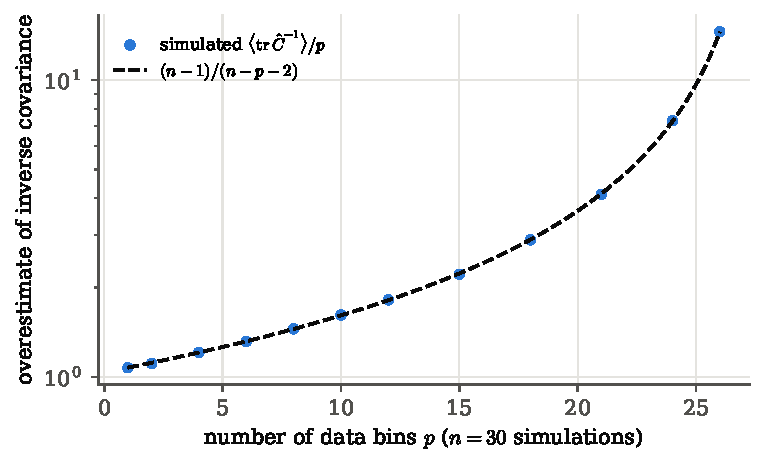
\includegraphics[width=10cm]{figures/ch03/hartlap.pdf}
\caption{How much the inverse of a sample covariance matrix overestimates
the true inverse, for thirty simulations and a growing number of bins
(logarithmic vertical axis). The simulated overestimate follows
$(n-1)/(n-p-2)$ (dashed): small for a few bins, a factor of two by
$p\approx14$, and diverging as $p$ approaches $n-2$.}
\label{3a:fig:hartlap}
\end{figure}

\begin{pitfall}[Selected and misread correlations]
A correlation coefficient estimated from the same data that were used to
choose which pair to look at is not distributed as
\eqref{3a:eq:fisher-z-dist}. Nor is a correlation evidence of a causal link,
and a zero correlation does not mean independence (the correlation only
sees the linear part of a relation, \cref{ch:02}).
\end{pitfall}

\paragraph{What this bought us.}
A covariance matrix estimated from $n$ samples has element-wise noise of
relative size $\sim1/\sqrt{n-1}$, which shows up as spurious correlations of
that size. Put error bars on a correlation in the variable
$z=\operatorname{artanh}r$, where the width is $1/\sqrt{n-3}$. Before
inverting an estimated covariance, multiply the inverse by the Hartlap
factor $(n-p-2)/(n-1)$, and choose $n$ well above $p$.

\paragraph{Verification and research.}
Everything above was verified against formulas valid for Gaussian
readings. For band powers from masked skies or non-Gaussian fields, neither
\eqref{3a:eq:var-cov-element} nor \eqref{3a:eq:hartlap} is exact, and the
number of simulations needed for a stable $\chi^2$ is itself found by
simulation: rerun the covariance estimate with independent sets of
simulations and watch how the parameter constraints move (\cref{ch:08}).

\section{Propagating errors through a formula}
\label{3a:sec:propagation}

The pendulum student now measures the length, $L=1.000\pm0.002\,$m, and the
period, $T=2.006\pm0.004\,$s, and computes $g=4\pi^2L/T^2$. What is the error
on $g$? A particle physicist asks the same about a branching ratio
$N_{\text{signal}}/N_{\text{norm}}$, a cosmologist about $H_0$ derived from a
measured angle and a sound horizon. And sometimes the textbook answer is badly
wrong: a ratio whose denominator is poorly measured has a distribution with
tails that no Gaussian error bar describes.

Faced with a formula and a few uncertain inputs, the tempting non-answer is the one in
\cref{3a:fig:ebeb}: we are not sure how big the error on each point is, so we give the error
bar an error bar of its own, and that one an error bar too. It never ends in a number. The
way out is to notice that the uncertainty of $g$ is not a new, separate unknown. It is the
uncertainty of $L$ and $T$, carried once through the formula $g=4\pi^2L/T^2$. The rest of this
section shows how.

\begin{figure}[htbp]
\centering
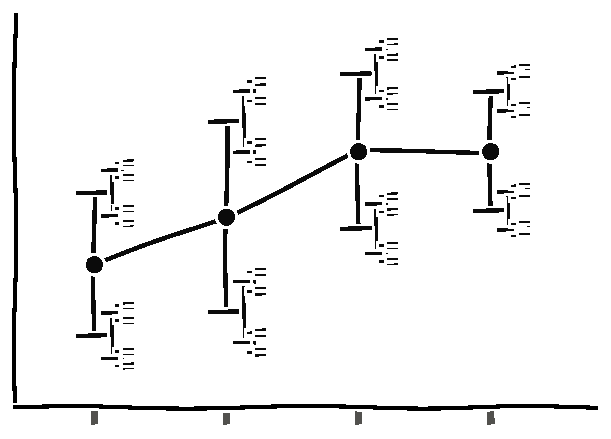
\includegraphics[width=0.62\linewidth]{figures/ch03/error_bars_on_error_bars.pdf}
\caption{What not propagating an error looks like: every error bar gets error bars of its own,
three levels deep, and the picture never settles to one number per point.}
\label{3a:fig:ebeb}
\end{figure}

The standard answer replaces the formula by its tangent, which gives the
output covariance as a ``Jacobian sandwich'' $A\Cmat A\T$ and shows exactly
where correlations between the inputs enter. The answer is exact for linear
formulas, and right for large samples (the delta method). Where it fails, a
Monte Carlo propagation still works.

\paragraph{Every smooth function is linear up close.}
Zoom in on a smooth curve and it looks like its tangent line. If the cloud of
possible input values is small compared with the scale on which the function
bends, then over that cloud the function is effectively linear, and a linear
map sends a Gaussian to a Gaussian, stretched by the slope. When the cloud is
wide enough to feel the curvature, the output is skewed and its centre
shifts. Near a pole, like $1/x$ at $x=0$, all bets are off.

\paragraph{What we want to know.}
\begin{enumerate}[label=\arabic*.]
  \item Given the means and covariance of the inputs, what are the mean and
        covariance of the outputs, to the first order in the fluctuations?
  \item When is that answer exact, and when is it an approximation?
  \item How do correlations between inputs change the result?
  \item How can we tell that the approximation has failed, and what then?
\end{enumerate}

\begin{figure}[htbp]
\centering
\begin{tikzpicture}
\begin{axis}[width=9cm,height=6cm,xmin=0.4,xmax=3.0,ymin=0,ymax=1.6,
  xlabel={input $x$},ylabel={output $y=1/x$},samples=200,
  tick label style={font=\footnotesize},label style={font=\small},
  clip=false]
  \addplot[very thick,formblue,domain=0.62:3.0] {1/x};
  \addplot[thick,tangentgreen,domain=0.7:2.6] {1/1.5-(x-1.5)/2.25};
  \draw[fibreorange,dashed] (axis cs:1.2,0) -- (axis cs:1.2,0.8333) -- (axis cs:0.4,0.8333);
  \draw[fibreorange,dashed] (axis cs:1.8,0) -- (axis cs:1.8,0.5556) -- (axis cs:0.4,0.5556);
  \draw[softgray,dotted,thick] (axis cs:1.5,0) -- (axis cs:1.5,0.6667) -- (axis cs:0.4,0.6667);
  \fill[fibreorange] (axis cs:1.2,0.8333) circle (1.6pt);
  \fill[fibreorange] (axis cs:1.8,0.5556) circle (1.6pt);
  \fill[tangentgreen] (axis cs:1.2,0.8) circle (1.6pt);
  \fill[tangentgreen] (axis cs:1.8,0.5333) circle (1.6pt);
  \addplot[thick,bdryred,domain=0.6:2.4] {0.35*exp(-(x-1.5)^2/(2*0.09))};
  \node[anchor=west,font=\footnotesize,formblue] at (axis cs:1.05,1.3) {$y=1/x$};
  \node[anchor=west,font=\footnotesize,tangentgreen] at (axis cs:2.2,0.18) {tangent at $\mu$};
  \node[anchor=east,font=\footnotesize,bdryred] at (axis cs:0.85,0.2) {input density};
\end{axis}
\end{tikzpicture}
\caption{Linear propagation through $y=1/x$ with input $\mu=1.5$,
$\sigma=0.3$. The red curve is the input density. Orange dots: the true
images of $\mu\pm\sigma$, at $0.556$ and $0.833$, lie asymmetrically about the
image $0.667$ of the mean (dotted). Green dots: the tangent line puts them
symmetrically at $0.533$ and $0.800$. The curvature makes the output skewed
towards large $y$, which is what the Monte Carlo shows later.}
\label{3a:fig:tangent}
\end{figure}

\subsection{The first-order formula}
\label{3a:sec:linear-propagation}

Let the inputs $\bm x=(x_1,\dots,x_n)$ have means $\bm\mu$ and covariance
matrix $V_{ij}=\Cov(x_i,x_j)$, and let $y(\bm x)$ be a smooth function. Expand
about the means,
\begin{equation}
  y(\bm x)=y(\bm\mu)+\sum_{i=1}^n\frac{\partial y}{\partial x_i}\Big|_{\bm\mu}(x_i-\mu_i)
  +\frac12\sum_{i,j}\frac{\partial^2y}{\partial x_i\partial x_j}\Big|_{\bm\mu}(x_i-\mu_i)(x_j-\mu_j)+\cdots,
  \label{3a:eq:taylor}
\end{equation}
If the inputs scatter only a little about their means, the quadratic and
higher terms are small, so we keep only the linear term. Write
$g_i=\partial y/\partial x_i$ at $\bm\mu$. Then, to this order,
\begin{align}
  \E y &\eqby{1} y(\bm\mu)+\sum_ig_i\,\E(x_i-\mu_i) \eqby{2} y(\bm\mu),
  \label{3a:eq:prop-mean}\\
  \sigma_y^2=\E\bigl[(y-\E y)^2\bigr]
  &\eqby{3} \E\Bigl[\Bigl(\sum_ig_i(x_i-\mu_i)\Bigr)^2\Bigr]
   \eqby{4} \sum_{i,j}g_ig_j\,\E\bigl[(x_i-\mu_i)(x_j-\mu_j)\bigr]
   \eqby{5} \sum_{i,j}g_i\,V_{ij}\,g_j .
  \label{3a:eq:prop-var}
\end{align}
\begin{explain}
  \item Take the expectation of the linearised \eqref{3a:eq:taylor}. The $g_i$ are constants.
  \item Each $\E(x_i-\mu_i)=0$.
  \item Subtract \eqref{3a:eq:prop-mean} from the linearised $y$.
  \item Square of a sum is a double sum, then linearity.
  \item Definition of the covariance.
\end{explain}
For several outputs $y_1,\dots,y_m$, the same steps with two different
outputs $y_k,y_l$ give the covariance matrix of the outputs,
\begin{equation}
  U_{kl}=\Cov(y_k,y_l)\approx\sum_{i,j}\frac{\partial y_k}{\partial x_i}\frac{\partial y_l}{\partial x_j}V_{ij},
  \qquad
  U=A\,V\!A\T,\qquad A_{ki}=\frac{\partial y_k}{\partial x_i}\Big|_{\bm\mu},
  \label{3a:eq:prop-matrix}
\end{equation}
where $A$ is the $m\times n$ \newterm{Jacobian} matrix
\srcref{Cowan}{(1.53)--(1.56)}.

\begin{workdef}[linear error propagation]
\newterm{Linear} (first-order) \newterm{error propagation} replaces each
function by its tangent plane at the input means \unpack{the first two terms
of the Taylor series, valid when the inputs scatter over a region where the
second derivatives hardly matter}, so that the output covariance is
$U=AVA\T$ with $A$ the Jacobian at the means. If the inputs are
uncorrelated, $V$ is diagonal and
$\sigma_y^2=\sum_i(\partial y/\partial x_i)^2\sigma_i^2$
\srcref{Cowan}{(1.57)}.
\end{workdef}

\paragraph{Four rules everybody uses.}
With two inputs and $V_{12}=\rho\sigma_1\sigma_2$, \eqref{3a:eq:prop-var}
gives \srcref{Cowan}{(1.59)--(1.60)}:
\begin{align}
  y=x_1\pm x_2:&\quad \sigma_y^2=\sigma_1^2+\sigma_2^2\pm2\rho\sigma_1\sigma_2,
  \label{3a:eq:prop-sum}\\
  y=x_1x_2\ \text{or}\ x_1/x_2:&\quad
  \frac{\sigma_y^2}{y^2}=\frac{\sigma_1^2}{x_1^2}+\frac{\sigma_2^2}{x_2^2}\pm\frac{2\rho\sigma_1\sigma_2}{x_1x_2},
  \label{3a:eq:prop-product}\\
  y=x^k:&\quad \frac{\sigma_y}{|y|}=|k|\,\frac{\sigma_x}{|x|},
  \label{3a:eq:prop-power}\\
  y=\ln x:&\quad \sigma_y=\frac{\sigma_x}{x}.
  \label{3a:eq:prop-log}
\end{align}
(For the product take $+$, for the ratio $-$. The derivatives are
$\partial(x_1x_2)/\partial x_1=x_2$, $\partial(x_1/x_2)/\partial x_2=-x_1/x_2^2$,
and dividing by $y^2$ turns them into relative errors.) Absolute errors add
in quadrature for sums, relative errors for products and ratios.

\paragraph{Example: The pendulum.}
\label{3a:ex:pendulum-prop}
$g=4\pi^2LT^{-2}$ is a product of powers, so relative errors add in
quadrature with weights $|k|$:
\begin{align*}
  \frac{\sigma_g^2}{g^2}
  &\eqby{1} \Bigl(\frac{\sigma_L}{L}\Bigr)^2+\Bigl(2\,\frac{\sigma_T}{T}\Bigr)^2
   \eqby{2} (0.002)^2+\Bigl(\frac{2\times0.004}{2.006}\Bigr)^2
   = 4.0\times10^{-6}+1.59\times10^{-5},\\
  g &\eqby{3} \frac{4\pi^2\times1.000}{2.006^2}=\ThreeAPendG\ \mathrm{m\,s^{-2}},\qquad
  \sigma_g=\ThreeAPendG\times\sqrt{1.99\times10^{-5}}=\ThreeAPendSgLin\ \mathrm{m\,s^{-2}}.
\end{align*}
\begin{explain}
  \item \eqref{3a:eq:prop-product} and \eqref{3a:eq:prop-power} with $k=1$ for $L$
        and $k=-2$ for $T$. $L$ and $T$ are measured independently, so $\rho=0$.
  \item Insert the numbers.
  \item The central value is the function at the input means \eqref{3a:eq:prop-mean}.
\end{explain}
The period dominates. Its relative error ($0.20\%$) is the same as that of
$L$, but it enters squared, so it contributes four times the variance. To
improve $g$, time more swings.

\paragraph{Example: A common calibration: correlated errors.}
\label{3a:ex:common-calib}
Two energies $E_1,E_2$ are measured with the same calorimeter. Each has an
independent statistical error $\sigma_s$ and they share one calibration error
$\sigma_c$: $E_i=E_i^{\text{true}}+\epsilon_i+\delta$, where the $\epsilon_i$ are
independent with mean $0$ and variance $\sigma_s^2$, and the common shift
$\delta$, independent of both, has mean $0$ and variance $\sigma_c^2$. Then
$V_{11}=V_{22}=\sigma_s^2+\sigma_c^2$ and $V_{12}=\Cov(\epsilon_1+\delta,\epsilon_2+\delta)=\sigma_c^2$.
For the difference and the sum, \eqref{3a:eq:prop-sum} gives
\begin{align*}
  \Var(E_1-E_2) &\eqby{1} 2(\sigma_s^2+\sigma_c^2)-2\sigma_c^2=2\sigma_s^2,\qquad
  \Var(E_1+E_2) \eqby{2} 2(\sigma_s^2+\sigma_c^2)+2\sigma_c^2=2\sigma_s^2+4\sigma_c^2 .
\end{align*}
\begin{explain}
  \item Minus sign: the common shift $\delta$ cancels in a difference.
  \item Plus sign: it adds coherently in a sum, so its standard deviation doubles.
\end{explain}
Ignoring the correlation would overstate the error of a mass difference and
understate the error of a total energy. This is why experiments publish full
covariance matrices, not just error bars.

\subsection{Linear maps are exact, and every covariance can be diagonalised}
\label{3a:sec:linear-exact}

If $\bm y=A\bm x$ exactly (a linear map, as in a change of basis, a
rebinning, or a sum of channels), there is no Taylor remainder, and
\begin{align}
  U_{kl}=\Cov(y_k,y_l)
  &\eqby{1} \E\Bigl[\sum_iA_{ki}(x_i-\mu_i)\sum_jA_{lj}(x_j-\mu_j)\Bigr]
   \eqby{2} \sum_{i,j}A_{ki}V_{ij}A_{lj}
   = (AVA\T)_{kl}
  \label{3a:eq:linear-exact}
\end{align}
\begin{explain}
  \item $y_k-\E y_k=\sum_iA_{ki}(x_i-\mu_i)$ by linearity, with no approximation.
  \item Multiply out and use linearity of expectation.
\end{explain}
holds exactly \srcref{Cowan}{(1.62)}. A linear map of a Gaussian vector is
Gaussian, so for Gaussian inputs the whole distribution of $\bm y$ is
$\Normal(A\bm\mu,AVA\T)$.

Exactness has a useful consequence: a well-chosen linear map removes all
correlations. $V$ is real and symmetric, so it has $n$
orthonormal eigenvectors $\bm r^{(k)}$ with $V\bm r^{(k)}=\lambda_k\bm r^{(k)}$
and $\bm r^{(k)}\cdot\bm r^{(l)}=\delta_{kl}$. Take the rows of $A$ to be these
eigenvectors, $A_{ki}=r^{(k)}_i$. Then
\begin{align}
  U_{kl}
  &\eqby{1} \sum_{i,j}r^{(k)}_iV_{ij}r^{(l)}_j
   \eqby{2} \sum_ir^{(k)}_i\,\lambda_l\,r^{(l)}_i
   \eqby{3} \lambda_l\,\delta_{kl} .
  \label{3a:eq:decorrelate}
\end{align}
\begin{explain}
  \item \eqref{3a:eq:linear-exact} with $A_{ki}=r^{(k)}_i$.
  \item $\sum_jV_{ij}r^{(l)}_j=\lambda_lr^{(l)}_i$, the eigenvalue equation.
  \item Orthonormality of the eigenvectors.
\end{explain}
The new variables $y_k=\bm r^{(k)}\cdot\bm x$ are uncorrelated, with variances
equal to the eigenvalues of $V$ \srcref{Cowan}{(1.63)--(1.65)}. This is the
statistics version of finding normal modes of coupled oscillators, and
of the principal axes of an inertia tensor.

\paragraph{Example: Decorrelating two measurements.}
\label{3a:ex:decorrelate}
For $V=\sigma^2\begin{pmatrix}1&\rho\\\rho&1\end{pmatrix}$ the eigenvectors are
$(1,1)/\sqrt2$ and $(1,-1)/\sqrt2$ with eigenvalues $\sigma^2(1\pm\rho)$ (check:
$V(1,1)\T=\sigma^2(1+\rho)(1,1)\T$). The combinations $(x_1+x_2)/\sqrt2$ and
$(x_1-x_2)/\sqrt2$ are uncorrelated, and with $\rho$ close to $1$ the
difference is much better measured than either input. The calibration example
above is this with $\rho=\sigma_c^2/(\sigma_s^2+\sigma_c^2)$.

\subsection{The delta method: why the first-order formula is right for large samples}
\label{3a:sec:delta}

Linear propagation is an approximation, so when can we trust it? When the
inputs are themselves estimators built from $n$ readings. Their scatter then
shrinks like $1/\sqrt n$, the cloud of inputs shrinks onto the tangent, and
the curvature terms become negligible. The delta method makes this precise.

\paragraph{The delta method.}
If $\sqrt n(Y_n-\mu)\rightsquigarrow\Normal(0,\sigma^2)$ and $g$ is
differentiable with $g'(\mu)\neq0$, then
\begin{equation}
  \sqrt n\bigl(g(Y_n)-g(\mu)\bigr)\rightsquigarrow\Normal\bigl(0,\ g'(\mu)^2\sigma^2\bigr),
  \qquad\text{i.e.}\qquad g(Y_n)\approx\Normal\Bigl(g(\mu),\ \frac{g'(\mu)^2\sigma^2}{n}\Bigr).
  \label{3a:eq:delta}
\end{equation}
For a vector, $\sqrt n\bigl(g(\bm Y_n)-g(\bm\mu)\bigr)\rightsquigarrow
\Normal\bigl(0,\nabla g\T\bm\Sigma\nabla g\bigr)$ \mainref{Thms.~5.13, 5.15}.

Why it is true: expand $g(Y_n)=g(\mu)+g'(\mu)(Y_n-\mu)+R_n$ with a remainder
$R_n$ of order $(Y_n-\mu)^2$. Multiply by $\sqrt n$. The linear term
$g'(\mu)\sqrt n(Y_n-\mu)$ tends in distribution to $\Normal(0,g'(\mu)^2\sigma^2)$.
The remainder is $\sqrt n\,R_n\sim\sqrt n\,(Y_n-\mu)^2=[\sqrt n(Y_n-\mu)]^2/\sqrt n$,
a quantity of fixed size divided by $\sqrt n$, so it tends to zero in
probability, and Slutsky's theorem lets us drop it. The curvature does not
disappear. It becomes negligible compared with the shrinking linear scatter.

\paragraph{Example: A function of one mean, and the product of two.}
\label{3a:ex:delta}
In both cases the inputs are sample means, so by the central limit theorem
$\sqrt n(\bar X_n-\mu)\rightsquigarrow\Normal(0,\sigma^2)$ and the delta
method applies. (a) For $W_n=e^{\bar X_n}$, $g(s)=e^s$ has
$g'(\mu)=e^\mu$, so $W_n\approx\Normal(e^\mu,e^{2\mu}\sigma^2/n)$
\mainref{Ex.~5.14}. (b) For the product of two means,
$Y=\bar X_1\bar X_2$ from $n$ paired readings with covariance matrix
$\bm\Sigma=(\sigma_{ab})$, the gradient of $g(s_1,s_2)=s_1s_2$ at $\bm\mu$ is
$(\mu_2,\mu_1)$ and
\begin{align*}
  \nabla g\T\bm\Sigma\nabla g
  &\eqby{1} \begin{pmatrix}\mu_2&\mu_1\end{pmatrix}
            \begin{pmatrix}\sigma_{11}&\sigma_{12}\\\sigma_{12}&\sigma_{22}\end{pmatrix}
            \begin{pmatrix}\mu_2\\\mu_1\end{pmatrix}
   \eqby{2} \mu_2^2\sigma_{11}+2\mu_1\mu_2\sigma_{12}+\mu_1^2\sigma_{22},
\end{align*}
\begin{explain}
  \item $\partial(s_1s_2)/\partial s_1=s_2$ and $\partial(s_1s_2)/\partial s_2=s_1$, at the means.
  \item Multiply out the quadratic form.
\end{explain}
so $\sqrt n(\bar X_1\bar X_2-\mu_1\mu_2)\rightsquigarrow\Normal(0,\mu_2^2\sigma_{11}+2\mu_1\mu_2\sigma_{12}+\mu_1^2\sigma_{22})$
\mainref{Ex.~5.16}. Dividing by $(\mu_1\mu_2)^2$ this is the product rule
\eqref{3a:eq:prop-product}.

\paragraph{When the slope vanishes.}
If $g'(\mu)=0$, the first-order formula says $\sigma_y=0$, which is absurd.
The second-order term takes over \srcref{CasellaBerger}{Thm.~5.5.26}: with
$g(Y_n)-g(\mu)\approx\frac12g''(\mu)(Y_n-\mu)^2$ and
$n(Y_n-\mu)^2/\sigma^2\rightsquigarrow\chi^2_1$,
\begin{equation}
  n\bigl(g(Y_n)-g(\mu)\bigr)\rightsquigarrow\frac{\sigma^2g''(\mu)}{2}\,\chi^2_1 .
  \label{3a:eq:second-order-delta}
\end{equation}
Estimating a power $|A|^2$ when the true amplitude $A$ is zero is exactly this
case. With $g(s)=s^2$ we have $g'(0)=0$ and $g''=2$, so the estimate is
$\sigma^2\chi^2_1/n$: never negative, and biased upward by $\sigma^2/n$
(the mean of $\chi^2_1$ is $1$).

\paragraph{The second-order bias.}
Keeping the quadratic term of \eqref{3a:eq:taylor} in the mean gives
$\E y\approx y(\bm\mu)+\frac12\sum_{ij}\partial_i\partial_jy\,V_{ij}$. For
$y=1/x$ this is $\E(1/x)\approx\frac1\mu\bigl(1+\sigma^2/\mu^2\bigr)$, always
above $1/\mu$, as \cref{3a:fig:tangent} suggests. For the ratio of means
$\bar X/\bar Y$ Casella and Berger derive in the same way
\srcref{CasellaBerger}{Ex.~5.5.27}
\[
  \E\frac{\bar X}{\bar Y}\approx\frac{\mu_X}{\mu_Y},\qquad
  \Var\frac{\bar X}{\bar Y}\approx\frac1n\,\frac{\mu_X^2}{\mu_Y^2}
  \Bigl(\frac{\sigma_X^2}{\mu_X^2}+\frac{\sigma_Y^2}{\mu_Y^2}-\frac{2\sigma_{XY}}{\mu_X\mu_Y}\Bigr),
\]
the ratio rule \eqref{3a:eq:prop-product} with $\sigma^2\to\sigma^2/n$, and
they warn that it can be far off when $\mu_Y$ is near zero.

\subsection{When linear propagation fails: the ratio of Gaussians}
\label{3a:sec:ratio}

Let $x_1\sim\Normal(\mu_1,\sigma_1^2)$ and $x_2\sim\Normal(\mu_2,\sigma_2^2)$ be
independent and $y=x_1/x_2$. The linear rule gives a Gaussian of width
$\sigma_y=|y_0|\sqrt{(\sigma_1/\mu_1)^2+(\sigma_2/\mu_2)^2}$ around
$y_0=\mu_1/\mu_2$. But the denominator has a nonzero density at $x_2=0$,
where $y$ diverges, so $y$ has no mean and no variance at all, however small
$\sigma_2/\mu_2$ is. The extreme case, both means zero, shows where the
heavy tails come from.

\paragraph{Example: The ratio of two zero-mean Gaussians is a Breit--Wigner.}
\label{3a:ex:ratio-cauchy}
Let $x_1,x_2\sim\Normal(0,1)$ independently. The pair $(x_2,x_1)$ is an
isotropic Gaussian in the plane, so its polar angle $\Theta$ is uniformly
distributed, and $y=x_1/x_2=\tan\Theta$. Since $\tan$ has period $\pi$, we can
take $\Theta$ uniform on $(-\pi/2,\pi/2)$. Then
\begin{align*}
  \Prob(y\le t)
  &\eqby{1} \Prob(\Theta\le\arctan t)
   \eqby{2} \frac{\arctan t+\pi/2}{\pi},\qquad
  f(t) \eqby{3} \frac{1}{\pi(1+t^2)} .
\end{align*}
\begin{explain}
  \item $\tan$ is increasing on $(-\pi/2,\pi/2)$.
  \item Uniform distribution on an interval of length $\pi$.
  \item Differentiate: $\frac{\dd}{\dd t}\arctan t=1/(1+t^2)$.
\end{explain}
This is the Cauchy (Breit--Wigner) distribution of \cref{3a:ex:cauchy}
\srcref{CasellaBerger}{\S5.5}. For $\mu_2\neq0$ the ratio keeps a
Cauchy-like $1/y^2$ tail. Its weight is set by how much probability $x_2$
has near zero.

\pyfile[firstline=39,lastline=51]{code/ch03/06_error_propagation.py}{Monte Carlo propagation for a ratio of Gaussians}

The script takes $\mu_1=10$, $\sigma_1=\sigma_2=1$ and three denominators,
$\mu_2=10,3,1$ (relative error $0.1$, $0.33$, $1$). For each it draws
$10^6$ pairs, forms the ratio, and compares the Monte Carlo distribution with
the linear prediction. Because the variance may not exist, it measures the
width by the half-distance between the $15.9$ and $84.1$ percentiles (which
is $\sigma$ for a Gaussian), and it counts negative ratios and ``$5\sigma$''
outliers.

\begin{table}[htbp]
\centering\small
\begin{tabular}{@{}lccc@{}}
\toprule
& $\sigma_2/\mu_2=0.1$ & $0.33$ & $1$\\
\midrule
linear prediction $y_0\pm\sigma_y$ & $1\pm\ThreeARatioALin$ & $3.33\pm\ThreeARatioBLin$ & $10\pm\ThreeARatioCLin$\\
Monte Carlo median & $\ThreeARatioAMed$ & $\ThreeARatioBMed$ & $\ThreeARatioCMed$\\
Monte Carlo central-68\% half-width & $\ThreeARatioAHalf$ & $\ThreeARatioBHalf$ & $\ThreeARatioCHalf$\\
fraction with $y<0$ & $\ThreeARatioANeg$ & $\ThreeARatioBNeg$ & $\ThreeARatioCNeg$\\
fraction beyond $5\sigma_y$ (Gaussian: $5.7\times10^{-7}$) & $\ThreeARatioAFar$ & $\ThreeARatioBFar$ & $\ThreeARatioCFar$\\
\bottomrule
\end{tabular}
\caption{Linear propagation against Monte Carlo for $y=x_1/x_2$.}
\label{3a:tab:ratio}
\end{table}

At 10\% relative error the linear rule is fine in the core (width
$\ThreeARatioAHalf$ against $\ThreeARatioALin$) but already has $300$ times
too many $5\sigma$ outliers. At 33\% the core is 12\% wider than predicted
and 3\% of ratios are beyond ``$5\sigma$''. At 100\% the linear answer is
meaningless: the median is $\ThreeARatioCMed$, not $10$, and $\ThreeARatioCNeg$
of the ratios are negative although both means are positive.

\begin{figure}[htbp]
\centering
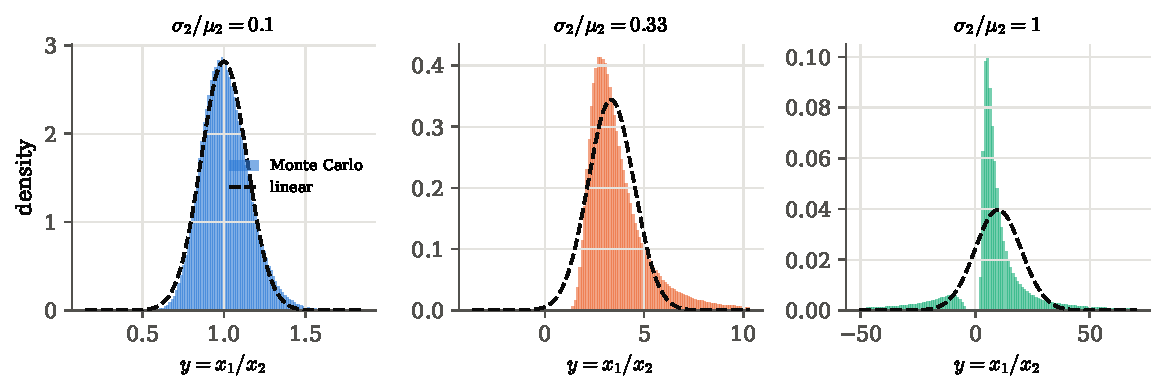
\includegraphics[width=12.5cm]{figures/ch03/ratio_failure.pdf}
\caption{The ratio of two Gaussian quantities, simulated (histograms) and by
linear propagation (dashed), as the denominator's relative error grows from
left to right. At 10\% the two agree. At 33\% the true distribution is
skewed, with a long right tail. At 100\% it has a spike near zero, negative
values and heavy tails, and bears no resemblance to the Gaussian.}
\label{3a:fig:ratio-failure}
\end{figure}

\begin{figure}[htbp]
\centering
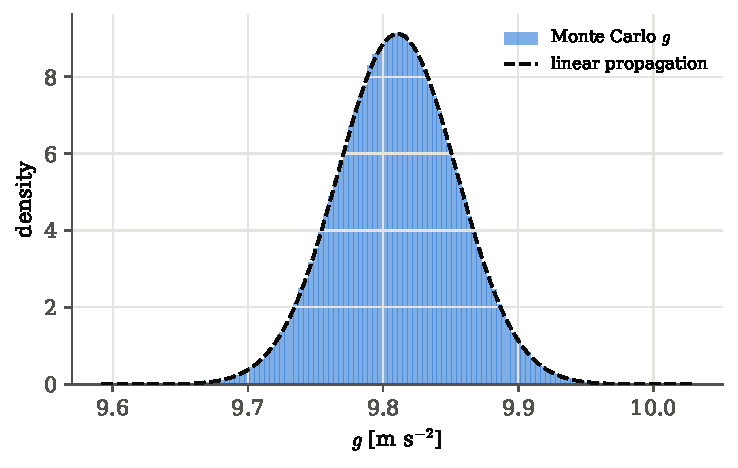
\includegraphics[width=7.5cm]{figures/ch03/pendulum_mc.pdf}
\caption{Monte Carlo propagation for the pendulum. A million pairs
$(L,T)$ drawn from their Gaussian errors give the histogram of $g$. The
linear-propagation Gaussian (dashed) lies on top of it, because the relative
errors of $0.2\%$ are tiny compared with the scale on which $L/T^2$ bends.}
\label{3a:fig:pendulum-mc}
\end{figure}

For the pendulum, by contrast, the Monte Carlo spread of $g$ is
$\ThreeAPendSgMC$ against the linear $\ThreeAPendSgLin$, and the mean is
$\ThreeAPendMeanMC$ (\cref{3a:fig:pendulum-mc}).

\begin{taxonomy}[Which propagation to use]
\centering\small
\begin{tabularx}{\linewidth}{@{}XX@{}}
\toprule
situation & method\\
\midrule
linear function ($\bm y=A\bm x$) & $U=AVA\T$, exact\\
small relative errors, smooth $y$ & first-order formula; check one case by Monte Carlo\\
$y$ depends on a quantity whose error is not small (ratio, $1/x$, $\ln x$ near $0$) & Monte Carlo propagation: sample inputs, apply $y$, histogram; quote median and percentiles\\
$g'(\mu)=0$ at the input means & second-order delta method, $\chi^2_1$ shape\\
inputs from an MCMC chain & apply $y$ to every sample of the chain (\cref{ch:09})\\
\bottomrule
\end{tabularx}
\end{taxonomy}

\paragraph{Symmetric error bars on a ratio.}
An efficiency, a branching ratio or a signal-to-background ratio with a
poorly known denominator should not be quoted as ``central $\pm$ symmetric
error''. The median is shifted, the errors are asymmetric, and the tails are
long. Quote percentiles from a Monte Carlo propagation or, better, build a
likelihood for the ratio directly (second half of \cref{ch:03}), as
Cowan recommends \srcref{Cowan}{p.~22}.

\paragraph{What this bought us.}
To first order, covariances propagate as $U=AVA\T$ with the Jacobian $A$:
absolute errors add in quadrature for sums, relative errors for products,
and correlations add $\pm2\rho\sigma_1\sigma_2$ terms. The rule is exact for
linear maps and asymptotically right for smooth functions of estimators
(delta method). It fails when the input scatter reaches a region of strong
curvature or a pole, and then Monte Carlo propagation is the answer.

\begin{inpractice}[Verification and research]
For the pendulum, Monte Carlo propagation merely verifies the linear formula.
For a derived cosmological parameter (the age of the Universe from $H_0$,
$\Omega_m$ and $\Omega_\Lambda$; $S_8=\sigma_8\sqrt{\Omega_m/0.3}$), the same idea
is the working tool: take every sample of a posterior chain, compute the
derived quantity, and histogram it. No Jacobian is needed, and correlations
and nonlinearity are handled automatically (\cref{ch:09}).
\end{inpractice}

\section{Combining measurements of different quality: the weighted mean}
\label{3a:sec:weighted}

Eight laboratories have measured the same quantity $\mu$: a particle mass, a
lifetime, the Hubble constant. Their error bars range from $0.5$ to $3$ in
some unit. A reviewer asks for one number. The plain average treats the best
laboratory and the worst on an equal footing, and that feels wrong. A
measurement with a small error bar should count for more. But how much more,
and how small is the error of the combination?

One idea settles both questions with the tools we already
have. The combination is again an estimator, a recipe applied to the data,
so it has a sampling distribution, a bias and a variance
(\cref{3a:sec:sampling,3a:sec:bias-variance}). Among all unbiased linear
recipes we look for the one with the smallest variance. The answer is the
\newterm{inverse-variance weighted mean}, and the same answer drops out of
the Gaussian likelihood, which is our first glimpse of the second half of
the chapter. The questions, in order, are these.
\begin{enumerate}[label=\arabic*.]
  \item Which weights $w_i$ make $\sum_i w_ix_i$ unbiased with the smallest
        variance, and what is that variance?
  \item How can we check that the measurements agree well enough for the
        combination to mean something?
  \item What changes when the measurements are correlated, for example
        because they share a systematic error?
  \item What if the readings also contain something we do not want, which
        enters each of them differently? How do we remove it?
\end{enumerate}

\paragraph{When the readings carry more than the signal.}
The laboratories differ only in how noisy they are. Readings can also
differ in what they contain. At the start of the chapter we wrote every reading as a piece that responds
to what we want, plus everything else \eqref{3a:eq:hidden-s}. So far,
``everything else'' has been noise of a known kind: it scatters around zero
with a spread we can describe, and it is different in every reading. For
that we already have good tools. We average, the noise partly cancels, and
the error bar shrinks like $1/\sqrt N$.

Sometimes they carry something more than noise. Picture yourself at a
noisy party with two microphones, trying to record a friend. She stands
between them, so both pick up her voice equally loudly. A loudspeaker plays
music, and it stands closer to the second microphone, so there the music is
twice as loud. Averaging the two recordings does not help, because the music
is not random noise that averages away: it is the same song in both, only
louder in one. Yet there is a trick. Double the first recording and subtract
the second. The music, twice in each, cancels. The voice, twice minus once,
survives. Noise-cancelling headphones work on exactly this principle.

The sky does the same thing to an astronomer. The microwave background has
the same brightness at two observing frequencies, while the dust of our own
Galaxy is much brighter at the higher one. A calibration drift, a
contaminating source, a foreground: whenever the unwanted part has a pattern
of its own across the readings, different from the pattern of what we want,
we can weight the readings so that the unwanted pattern cancels and the
wanted one survives. Each reading gets its own weight, $F=\sum_iw_ix_i$, and
the question is which weights to use.

\emph{The party in symbols.} Call the voice (or the sky signal) $s$ and the
music (or the dust) $f$. It is twice as strong in the second reading, and
each reading has its own noise. Combine them with two numbers $w_1,w_2$:
\begin{align}
  x_1&=s+f+n_1,\qquad x_2=s+2f+n_2,\notag\\
  w_1x_1+w_2x_2&\eqby{1}(w_1+w_2)\,s+(w_1+2w_2)\,f+(w_1n_1+w_2n_2).
  \label{3a:eq:two-channel}
\end{align}
\begin{explain}
  \item Multiply out and collect the terms in $s$, in $f$ and in the noise.
\end{explain}
Each bracket is a dial. The first sets the \emph{normalisation}: unless
$w_1+w_2=1$ we are estimating a rescaled signal. The plain difference
$x_2-x_1=f+n_2-n_1$ shows how badly this can go: its weights sum to zero,
so the signal cancels completely and what is left measures the foreground.
The second bracket sets the \emph{contamination}: $w_1+2w_2=0$ removes $f$
whatever its value. Both conditions together fix the weights,
$w_1=2$, $w_2=-1$, and
\begin{equation}
  2x_1-x_2 \eqby{1} s+(2n_1-n_2),\qquad
  \Var(2x_1-x_2)\eqby{2}4\sigma_1^2+\sigma_2^2 .
  \label{3a:eq:two-channel-clean}
\end{equation}
\begin{explain}
  \item \eqref{3a:eq:two-channel} with $w_1+w_2=1$ and $w_1+2w_2=0$.
  \item Independent noises: variances add, each weighted by $w_i^2$
        \eqref{3a:eq:var-sum}.
\end{explain}
The foreground is gone exactly, the signal keeps its unit normalisation, and
the price is noise: with $\sigma_1=\sigma_2=\sigma$ the clean combination has
variance $5\sigma^2$, ten times the $\sigma^2/2$ of the plain average
$(x_1+x_2)/2$, which in exchange keeps $1.5f$ of foreground. Weights that
cancel unwanted pieces are easy to find; weights that also keep the noise
small are a trade-off. Lesson: a linear combination can switch off anything
whose response across the readings differs from that of $s$, while one
constraint, $\sum_iw_i=1$ for a signal that enters every reading equally,
keeps $s$ itself intact; the rest is the choice of the least noisy weights
among those allowed.

\paragraph{A picture: weights point in a direction.}
Write the two readings as one list, $\bm x=(x_1,x_2)\T$. The signal enters
both readings equally, with the pattern $\bm a=(1,1)\T$; the dust enters
with the pattern $\bm c=(1,2)\T$. The weights are a third list,
$\bm w=(w_1,w_2)\T$, and a weighted sum multiplies matching entries and adds
them up. That is a dot product, so the readings and the two dials become
\begin{equation}
  \bm x=\bm a\,s+\bm c\,f+\bm n
  \qquad\Longrightarrow\qquad
  \bm w\T\bm x\eqby{1}(\bm w\T\bm a)\,s+(\bm w\T\bm c)\,f+\bm w\T\bm n .
  \label{3a:eq:dials-vector}
\end{equation}
\begin{explain}
  \item Multiply each term by $\bm w\T$; a number in front of a list comes
        out of the dot product.
\end{explain}
For the weights $\bm w=(2,-1)\T$ the signal gives $2\cdot1-1\cdot1=1$ and
survives; the dust gives $2\cdot1-1\cdot2=0$ and vanishes. In the language
of geometry, $\bm w$ points at right angles to the dust's pattern, so it is
blind to the dust however bright it is.

\Cref{3a:fig:ruler} shows what the weighted sum does to a point. Lay a ruler
along $\bm w$, marked so that it reads $\bm w\T\bm x$, and drop the data
straight down onto it, at right angles. Where the point lands is the reading.
Because the ruler stands at right angles to everything else, sliding the
point in that direction does not move its shadow: the data and the signal
alone land on the same mark. Only the signal moves the shadow along the
ruler.

\begin{figure}[htbp]
\centering
\begin{tikzpicture}[x=1.75cm,y=1.75cm,font=\small,>={Stealth[length=7pt,width=5pt]}]
  \coordinate (O) at (0,0); \coordinate (S) at (2.2,0.88); \coordinate (E) at (0.48,1.6);
  \coordinate (X) at (2.68,2.48); \coordinate (W) at (1.136,-0.341);
  \coordinate (U) at (0.8077,-0.2424); \coordinate (R) at ($2.2*(U)$);
  \draw[black!30,->] (-0.4,0) -- (3.4,0) node[below left=1pt,black!55] {\footnotesize mic 1};
  \draw[black!30,->] (0,-1.0) -- (0,3.0) node[below left=1pt,black!55] {\footnotesize mic 2};
  \draw[black!55,line width=0.8pt] ($-0.4*(U)$) -- ($3.3*(U)$);
  \foreach \k in {1,2,3} \draw[black!55] ($\k*(U)+0.07*(0.3,1)$) -- ($\k*(U)-0.07*(0.3,1)$);
  \draw[bdryred!55,line width=1.2pt] (X) -- (R);
  \pic[draw=bdryred!70,line width=0.6pt,angle radius=0.22cm] {right angle=X--R--O};
  \fill[bdryred] (R) circle (1.6pt) node[below right=0pt,bdryred] {$s$};
  \draw[decorate,decoration={brace,mirror,amplitude=5pt,raise=11pt},bdryred!85!black,line width=0.7pt]
        (O) -- (R) node[midway,below=19pt,font=\footnotesize] {$\bm w\T\bm x$};
  \draw[->,formblue,line width=1.6pt] (O) -- (S);
  \draw[->,fibreorange,line width=1.6pt] (O) -- (E);
  \draw[->,black,line width=1.6pt] (O) -- (X);
  \draw[->,bdryred,line width=1.6pt] (O) -- (W);
  \node[formblue,above left=0pt] at ($(S)+(0,0.05)$) {signal};
  \node[fibreorange,left=1pt] at (E) {everything else};
  \node[black,above=1pt] at (X) {data};
  \node[bdryred,above right=-1pt] at (W) {$\bm w$};
\end{tikzpicture}
\caption{The weighted sum as a shadow on a ruler. The data are the signal plus everything else. The
weights $\bm w$ point along a ruler at right angles to everything else; the reading $\bm w\T\bm x$ is
where the data fall when dropped straight onto it. The tip of the signal lies on the same drop line, so
the data and the signal alone give the same reading. The two patterns are drawn further apart than at
the party, so that the angles are easy to see.}
\label{3a:fig:ruler}
\end{figure}

So $\bm w$ is a filter. It asks one question of the data: how much of the
pattern we want is here, ignoring everything else? Notice that it does not
point along the signal. It points where it must to be blind to everything
else, so its direction is set as much by what we ignore as by what we want;
only when the rest is plain noise does it line up with the signal itself. A
neuron in a network is the same kind of filter. Its weights also decide
which differences in the input it reads and which it ignores, but nobody
works them out: they start at random and are adjusted during training until
the readings are useful. Choosing weights is choosing a direction: one that
sees what we want and is blind to what we do not. With
more readings there is room to be blind to more unwanted patterns at once,
and finding the weights is a small set of linear equations. When the
unwanted patterns are not known exactly, or the noise matters as much as
they do, we look instead for the direction along which the combination
scatters least, and that search is the rest of this section.

\emph{The universal principle.} The two microphones did one thing: each
recording was the voice plus everything else, and the weights kept the voice
and dropped the rest. Every weighted sum in this section does the same, and
so, it turns out, does almost every analysis in the book. What makes it
possible is a \newterm{feature}: a property that the part we want has and
the rest does not. At the party it is how loud each source is in each
microphone: the voice equally loud in both, the music twice as loud in
one. Building a quantity that keeps the wanted feature and drops the others
is \newterm{feature extraction}, and the weighted sum is its simplest form.
The principle has one hard limit: without a feature there is no
separation. Put the loudspeaker right next to your friend, and voice and
music arrive equally loud in both microphones; no weights can pull them
apart, because weights can use a difference the data contain but cannot
invent one.

The principle does not stop at simple problems; even an artificial neural
network runs on it. Suppose someone has written the digit 9 on a sheet of
paper, we photograph it, and a network must tell from the photograph which
digit was written. The photograph is a grid of pixel values: the pixels of
the written 9, plus the paper, a smudge, uneven light. A first layer of
weighted sums extracts the feature we want, the pixels that belong to the
number. Those pixels are in turn a few shapes, a loop and a stroke running
down from it, plus details that do not matter, such as the size of the
loop; the next layer extracts the shapes. The last layers turn the shapes
into the answer: one loop alone is a 0, two loops stacked are an 8, a loop
on top with a tail below is a 9. Each layer is a set of weighted sums, each
bent by a fixed curve, and each takes what the layer before it kept as its
new data. The only real difference from our two microphones is where the
weights come from: a network learns them from many labelled examples, while
we work ours out from what we know about the patterns and the noise. So
even the most complicated network is a long chain of the step we have just
taken: isolate one feature, then the next. \Cref{3a:fig:network} writes it
with the same bookkeeping as the party, $\bm x=\bm a\,s+\bm c\,f+\bm n$:
at each step the data are split into the part we want plus the rest, and
weights keep the part we want.

\begin{figure}[htbp]
\centering
\def\loopcells{1/6,2/6,3/6,0/5,4/5,0/4,4/4,1/3,2/3,3/3,4/3}
\def\tailcells{4/2,4/1,2/0,3/0}
\newcommand\grid[3]{%
  \begin{scope}[shift={(#1,#2)},x=0.2cm,y=0.2cm]
    \fill[black!5] (0,0) rectangle (5,7); #3
    \draw[black!25,step=1] (0,0) grid (5,7);
  \end{scope}}
\newcommand\rest{\fill[softgray!55] (0,0) rectangle (2,1); \fill[softgray!35] (0,3) rectangle (1,4);}
\newcommand\cells[2]{\foreach \c/\r in #1 \fill[#2] (\c,\r) rectangle (\c+1,\r+1);}
\begin{tikzpicture}[font=\small,>=Stealth]
  \grid{0}{3.2}{\rest\cells{\loopcells}{formblue}\cells{\tailcells}{formblue}}
  \node at (1.35,3.9) {$=$};
  \grid{1.7}{3.2}{\cells{\loopcells}{formblue}\cells{\tailcells}{formblue}}
  \node at (3.05,3.9) {$+$};
  \grid{3.4}{3.2}{\rest}
  \node[below] at (0.5,3.2) {\footnotesize$\bm x$};
  \node[below] at (2.2,3.2) {\footnotesize$\bm x_9$};
  \node[below] at (3.9,3.2) {\footnotesize$\bm x_{\rm rest}$};
  \node[anchor=west,align=left,text width=6.2cm] at (5.0,3.9)
    {\footnotesize the photograph is the written 9 plus the paper, a smudge,
     uneven light; weights that match pen strokes keep $\bm x_9$};
  \grid{1.7}{0.9}{\cells{\loopcells}{formblue}\cells{\tailcells}{formblue}}
  \node at (3.05,1.6) {$=$};
  \grid{3.4}{0.9}{\cells{\loopcells}{fibreorange}}
  \node at (4.75,1.6) {$+$};
  \grid{5.1}{0.9}{\cells{\tailcells}{fibreorange}}
  \node[below] at (2.2,0.9) {\footnotesize$\bm x_9$};
  \node[below] at (3.9,0.9) {\footnotesize$\bm x_{\rm loop}$};
  \node[below] at (5.6,0.9) {\footnotesize$\bm x_{\rm tail}$};
  \node[anchor=west,align=left,text width=4.6cm] at (6.6,1.6)
    {\footnotesize the 9 is a loop plus a tail; weights that match each shape
     give its score};
  \newcommand\vbars[4]{%
    \begin{scope}[shift={(#1,#2)}]
      \draw[black!25] (0,0) rectangle (1.0,1.2);
      \foreach \v/\col [count=\k] in {#3} \fill[\col] (0.08,1.2-0.38*\k+0.06) rectangle ++(0.75*\v,0.26);
      \node[below] at (0.45,0) {\footnotesize #4};
    \end{scope}}
  \begin{scope}[yshift=-1.7cm]
    \node[anchor=east,align=right] at (1.7,1.01) {\footnotesize loop on top};
    \node[anchor=east,align=right] at (1.7,0.63) {\footnotesize tail below};
    \node[anchor=east,align=right] at (1.7,0.25) {\footnotesize second loop};
    \vbars{1.75}{0}{1.1/fibreorange,1.05/fibreorange,0.15/fibreorange}{$\bm s$}
    \node at (3.05,0.6) {$=$};
    \vbars{3.4}{0}{1/bdryred,1/bdryred,0/bdryred}{$\bm p_9$}
    \node at (4.75,0.6) {$+$};
    \vbars{5.1}{0}{0.1/softgray,0.05/softgray,0.15/softgray}{$\bm s_{\rm rest}$}
    \node[anchor=west,align=left,text width=5.4cm] at (6.6,0.6)
      {\footnotesize the shape scores are a 9's pattern plus a leftover;
       each digit's pattern $\bm p_d$ is its weights, its score is
       $\bm p_d\T\bm s$, and the 9 scores highest};
  \end{scope}
\end{tikzpicture}
\caption{Reading a handwritten 9 with the idea of the two microphones, used again and again. Each row
has the form \emph{data $=$ what we want $+$ the rest}, exactly like $\bm x=\bm a\,s+\bm c\,f+\bm n$,
and a set of weights keeps what we want: a weighted sum $\bm w\T\bm x$ whose weights match the wanted
pattern, bent by a fixed curve such as $\max(0,z)$. What one row keeps is the data of the next; in the
last row the data are the shape scores, and each digit's weights are its own pattern of shapes. A
neural network is this chain with many rows, and with weights learned from labelled examples.}
\label{3a:fig:network}
\end{figure}

Every step in the figure is the dot product of the two microphones, repeated
many times and chained; nothing else enters. Readings, patterns and weights
are all lists of numbers, so the natural language for all of it is linear
algebra.

We start with the simplest case: readings of different quality, no
contaminant, and weights chosen so the combination scatters as little as
possible. \Cref{3a:sec:weighted-corr} then lets the unwanted pieces be
shared between readings, and the same formula becomes the method used to
separate the microwave background from the Galaxy.

\subsection{The best linear combination}
\label{3a:sec:blue}

Let the measurements $x_1,\dots,x_N$ be independent, each unbiased,
$\E x_i=\mu$, with known standard deviations $\sigma_i$ that differ from one
measurement to the next. We try a \emph{linear} recipe
$\hat\mu=\sum_iw_ix_i$ with numbers $w_i$ still to be chosen. Two
properties follow at once:
\begin{align}
  \E\hat\mu &\eqby{1} \sum_i w_i\,\E x_i \eqby{2} \mu\sum_i w_i ,
  \label{3a:eq:wmean-bias}\\
  \Var\hat\mu &\eqby{3} \sum_i w_i^2\,\Var x_i \eqby{4} \sum_i w_i^2\sigma_i^2 .
  \label{3a:eq:wmean-var}
\end{align}
\begin{explain}
  \item Linearity of expectation.
  \item Every measurement is unbiased, $\E x_i=\mu$.
  \item Variance of a sum \eqref{3a:eq:var-sum}: the covariances vanish
        because the $x_i$ are independent, and a constant factor comes out
        squared, $\Var(wx)=w^2\Var x$.
  \item $\Var x_i=\sigma_i^2$.
\end{explain}
So $\hat\mu$ is unbiased for every value of $\mu$ exactly when the weights
sum to one, $\sum_iw_i=1$. Its mean squared error is then just its variance
\eqref{3a:eq:mse-decomp}, and we want the weights that make
$\sum_iw_i^2\sigma_i^2$ as small as possible under that one constraint.

\paragraph{Minimising with a Lagrange multiplier.}
Recall the method from mechanics: to minimise $f(\bm w)$ subject to
$g(\bm w)=0$, look for points where the gradient of $f$ is parallel to the
gradient of $g$, that is, where the gradient of
$f-\lambda g$ vanishes for some number $\lambda$ (the multiplier). Here
$f=\sum_iw_i^2\sigma_i^2$ and $g=\sum_iw_i-1$:
\begin{align}
  0 &\eqby{1} \frac{\partial}{\partial w_k}\Bigl[\sum_i w_i^2\sigma_i^2-\lambda\Bigl(\sum_iw_i-1\Bigr)\Bigr]
     \eqby{2} 2w_k\sigma_k^2-\lambda
  \quad\Longrightarrow\quad w_k=\frac{\lambda}{2\sigma_k^2},\notag\\
  1 &\eqby{3} \sum_k w_k = \frac{\lambda}{2}\sum_k\frac{1}{\sigma_k^2}
  \quad\Longrightarrow\quad \frac{\lambda}{2}=\frac{1}{W},
  \qquad W\equiv\sum_{k=1}^N\frac{1}{\sigma_k^2},\notag\\
  w_k &\eqby{4} \frac{1/\sigma_k^2}{W},\qquad
  \Var\hat\mu \eqby{5} \sum_k\frac{1}{\sigma_k^4W^2}\,\sigma_k^2
  = \frac{1}{W^2}\sum_k\frac{1}{\sigma_k^2}
  = \frac{1}{W}.
  \label{3a:eq:wmean-weights}
\end{align}
\begin{explain}
  \item Stationarity of $f-\lambda g$ in each $w_k$.
  \item Only the $i=k$ terms depend on $w_k$: $\partial(w_k^2\sigma_k^2)/\partial w_k=2w_k\sigma_k^2$
        and $\partial w_k/\partial w_k=1$.
  \item Impose the constraint $\sum_kw_k=1$ to fix $\lambda$.
  \item Insert $\lambda/2=1/W$ into $w_k=\lambda/(2\sigma_k^2)$.
  \item Insert these weights into \eqref{3a:eq:wmean-var}.
\end{explain}

A stationary point need not be a minimum. One inequality settles it: no
other unbiased linear recipe does better. For any weights with
$\sum_iw_i=1$, the Cauchy--Schwarz inequality
$(\sum_ia_ib_i)^2\le\sum_ia_i^2\sum_ib_i^2$ with $a_i=w_i\sigma_i$ and
$b_i=1/\sigma_i$ gives
\begin{equation}
  1 \eqby{1} \Bigl(\sum_i w_i\Bigr)^2
    \eqby{2} \Bigl(\sum_i w_i\sigma_i\cdot\frac{1}{\sigma_i}\Bigr)^2
    \relby{3}{\le} \sum_iw_i^2\sigma_i^2\;\sum_i\frac{1}{\sigma_i^2}
    \eqby{4} \Var\hat\mu\cdot W .
  \label{3a:eq:wmean-cs}
\end{equation}
\begin{explain}
  \item The weights sum to one.
  \item Multiply and divide each term by $\sigma_i$.
  \item Cauchy--Schwarz. Equality holds only when $a_i\propto b_i$, that is
        $w_i\sigma_i\propto1/\sigma_i$, or $w_i\propto1/\sigma_i^2$.
  \item \eqref{3a:eq:wmean-var} and the definition of $W$.
\end{explain}
So $\Var\hat\mu\ge1/W$ for every unbiased linear combination, and the
inverse-variance weights are the only ones that reach the bound.

\begin{workdef}[inverse-variance weighted mean]
For independent unbiased measurements $x_i$ of one quantity, with standard
deviations $\sigma_i$,
\[
  \hat\mu=\frac{\sum_ix_i/\sigma_i^2}{\sum_i1/\sigma_i^2},
  \qquad
  \sigma_{\hat\mu}=\Bigl(\sum_i\frac{1}{\sigma_i^2}\Bigr)^{-1/2}.
\]
Each measurement is weighted by its inverse variance $1/\sigma_i^2$
\unpack{a measurement twice as precise counts four times as much}. This is
the unbiased linear combination with the smallest variance
\srcref{Cowan}{(7.26)--(7.27)}, \srcref{Sivia}{(2.30)--(2.31)}.
\end{workdef}

\paragraph{What the formula says.}
Three consequences are worth reading off. First, since
$W\ge1/\sigma_k^2$ for every single $k$, the combined variance $1/W$ is
never larger than the smallest individual variance: adding a measurement,
however poor, never hurts \srcref{Cowan}{p.~107}. Second, if one
measurement is much more precise than the rest, it dominates both $W$ and
the weighted sum, and the combination is essentially that measurement.
Third, if all errors are equal, $\sigma_i=\sigma$, the weights are all
$1/N$ and $\Var\hat\mu=\sigma^2/N$, the familiar variance of the sample mean
\eqref{3a:eq:var-mean}.

Two pictures from physics make the formula feel familiar. Inverse variances
add like the conductances of resistors in parallel, $1/R=\sum_i1/R_i$: the
combined ``resistance to knowing $\mu$'' is smaller than the smallest
single one. And $\hat\mu$ is the centre of mass of the points $x_i$ with
masses $1/\sigma_i^2$; a precise measurement is a heavy mass that drags the
centre towards itself. Later we will call $1/\sigma^2$ the
\newterm{information} carried by a measurement, and the statement ``the
information of independent measurements adds'' becomes the additivity of
Fisher matrices (\cref{ch:10}).

\paragraph{The same answer from least squares and the likelihood.}
Suppose, in addition, that each $x_i$ is Gaussian,
$x_i\sim\Normal(\mu,\sigma_i^2)$. The probability density of the whole data
set, read as a function of $\mu$, is
$\prod_i(2\pi\sigma_i^2)^{-1/2}\exp[-(x_i-\mu)^2/2\sigma_i^2]$, so its
logarithm is a constant minus $\tfrac12\chi^2(\mu)$ with
\begin{equation}
  \chi^2(\mu)=\sum_{i=1}^N\frac{(x_i-\mu)^2}{\sigma_i^2}
  \label{3a:eq:wmean-chi2}
\end{equation}
\srcref{Cowan}{(7.25)}. Making the density as large as possible means making
$\chi^2$ as small as possible. We complete the square in $\mu$:
\begin{align}
  \chi^2(\mu)
  &\eqby{1} \sum_i\frac{x_i^2}{\sigma_i^2}-2\mu\sum_i\frac{x_i}{\sigma_i^2}+\mu^2\sum_i\frac{1}{\sigma_i^2}\notag\\
  &\eqby{2} \sum_i\frac{x_i^2}{\sigma_i^2}-2\mu W\hat\mu+\mu^2W\notag\\
  &\eqby{3} W(\mu-\hat\mu)^2+\Bigl[\sum_i\frac{x_i^2}{\sigma_i^2}-W\hat\mu^2\Bigr]
   \eqby{4} W(\mu-\hat\mu)^2+\chi^2_{\min}.
  \label{3a:eq:wmean-square}
\end{align}
\begin{explain}
  \item Expand $(x_i-\mu)^2=x_i^2-2\mu x_i+\mu^2$ and sum term by term.
  \item $\sum_ix_i/\sigma_i^2=W\hat\mu$ by the definition of the weighted
        mean, and $\sum_i1/\sigma_i^2=W$.
  \item Add and subtract $W\hat\mu^2$: $\mu^2W-2\mu W\hat\mu+W\hat\mu^2=W(\mu-\hat\mu)^2$.
  \item The bracket does not depend on $\mu$. It is the value of $\chi^2$ at
        $\mu=\hat\mu$, which we call $\chi^2_{\min}$.
\end{explain}
So $\chi^2$ is a parabola in $\mu$ with its minimum exactly at the weighted
mean \srcref{Cowan}{(7.26)}. Its curvature is
$\mathrm d^2\chi^2/\mathrm d\mu^2=2W$, and the density of the data, as a
function of $\mu$, is proportional to $\exp[-W(\mu-\hat\mu)^2/2]$: a
Gaussian bump of width $W^{-1/2}=\sigma_{\hat\mu}$. So the width of the
bump is exactly the error bar we derived from the sampling distribution.

Two more facts can be read off the parabola, and both return in the second
half of the chapter. First, the variance is ``two over the curvature of
$\chi^2$'': $\sigma_{\hat\mu}^2=1/W=2/(2W)$ \srcref{Cowan}{(7.27)},
\srcref{Sivia}{(2.31)}. Second, moving $\mu$ one standard error away from
$\hat\mu$ raises $\chi^2$ by exactly $1$, because $W\sigma_{\hat\mu}^2=1$.
The same formulas also appear as the peak and width of a Bayesian posterior
with a flat prior \srcref{Sivia}{pp.~30--31}. For Gaussian data and a flat
prior the two readings coincide.

\begin{keyidea}[Inverse-variance weighting]
To combine independent unbiased measurements, weight each by $1/\sigma_i^2$.
Inverse variances add: $1/\sigma_{\hat\mu}^2=\sum_i1/\sigma_i^2$. For
correlated measurements with covariance $V$, the weights become
$\bm w=V^{-1}\bm1/(\bm1\T V^{-1}\bm1)$ and
$1/\sigma_{\hat\mu}^2=\bm1\T V^{-1}\bm1$ (\cref{3a:sec:weighted-corr}).
\end{keyidea}

\paragraph{Example: two measurements of a mass.}
Two experiments report $x_1=10.0\pm0.3$ and $x_2=10.8\pm0.4$ (in
$\mathrm{GeV}$). The weights and the combination are
\begin{align*}
  \frac{1}{\sigma_1^2}&=\frac{1}{0.09}=11.11,\qquad
  \frac{1}{\sigma_2^2}=\frac{1}{0.16}=6.25,\qquad
  W\eqby{1}17.36,\\
  \hat\mu&\eqby{2}\frac{11.11\times10.0+6.25\times10.8}{17.36}
  =\frac{111.1+67.5}{17.36}=10.29,\qquad
  \sigma_{\hat\mu}\eqby{3}\frac{1}{\sqrt{17.36}}=0.24 .
\end{align*}
\begin{explain}
  \item $W$ is the sum of the inverse variances.
  \item Weighted mean. The first measurement carries weight $11.11/17.36=0.64$.
  \item $\sigma_{\hat\mu}=W^{-1/2}$.
\end{explain}
The result, $10.29\pm0.24$, is closer to the more precise measurement and is
more precise than either. The plain average $10.4$ would have the error
$\tfrac12\sqrt{0.09+0.16}=0.25$, slightly worse, and would be pulled
towards the poorer measurement.

\paragraph{Example: equal errors and one outstanding measurement.}
Take $N-1$ measurements with error $\sigma$ and one with error $\sigma/k$.
Then $W=(N-1)/\sigma^2+k^2/\sigma^2$, and the precise measurement carries the
weight
\begin{equation*}
  w_{\text{best}}\eqby{1}\frac{k^2/\sigma^2}{(N-1+k^2)/\sigma^2}
  =\frac{k^2}{N-1+k^2},
  \qquad
  \sigma_{\hat\mu}\eqby{2}\frac{\sigma}{\sqrt{N-1+k^2}} .
\end{equation*}
\begin{explain}
  \item \eqref{3a:eq:wmean-weights}, with the common factor $1/\sigma^2$ cancelled.
  \item $\sigma_{\hat\mu}=W^{-1/2}$.
\end{explain}
One measurement ten times more precise ($k=10$) is worth $k^2=100$ ordinary
ones: with $N-1=9$ ordinary measurements it carries $100/109=92\%$ of the
weight. Precision is worth its square.

\subsection{Do the measurements agree? The $\chi^2$ of the residuals}
\label{3a:sec:wchi2}

The error $\sigma_{\hat\mu}=W^{-1/2}$ uses only the quoted $\sigma_i$, never
the spread of the $x_i$ themselves. Two measurements $10.0\pm0.3$ and
$10.8\pm0.4$ give the same $\sigma_{\hat\mu}$ as $10.0\pm0.3$ and
$15.0\pm0.4$, although the second pair plainly contradicts itself. The value
of $\chi^2$ at its minimum is the missing check: it measures how far the
data scatter about $\hat\mu$ in units of their own error bars.

What value should we expect? Write $z_i=(x_i-\mu)/\sigma_i$ for the
standardised errors: they are independent with mean $0$ and variance $1$.
Then
\begin{align}
  \chi^2_{\min}
  &\eqby{1} \sum_i\frac{\bigl[(x_i-\mu)-(\hat\mu-\mu)\bigr]^2}{\sigma_i^2}\notag\\
  &\eqby{2} \sum_i z_i^2-2(\hat\mu-\mu)\sum_i\frac{x_i-\mu}{\sigma_i^2}+(\hat\mu-\mu)^2W\notag\\
  &\eqby{3} \sum_i z_i^2-2(\hat\mu-\mu)^2W+(\hat\mu-\mu)^2W
   = \sum_i z_i^2-W(\hat\mu-\mu)^2,\notag\\
  \E\chi^2_{\min}
  &\eqby{4} N-W\cdot\frac1W = N-1 .
  \label{3a:eq:wchi2-mean}
\end{align}
\begin{explain}
  \item Add and subtract the true $\mu$ inside $x_i-\hat\mu$.
  \item Expand the square. The first term is $z_i^2$, and $\sum_i1/\sigma_i^2=W$.
  \item $\sum_i(x_i-\mu)/\sigma_i^2=\sum_ix_i/\sigma_i^2-\mu W=W(\hat\mu-\mu)$.
  \item $\E z_i^2=1$ for each of the $N$ terms, and
        $\E(\hat\mu-\mu)^2=\Var\hat\mu=1/W$ because $\hat\mu$ is unbiased.
\end{explain}
This is the weighted twin of the $N-1$ in the sample variance
(\cref{3a:sec:n-minus-one}): fitting one parameter to the data uses up one
of the $N$ independent directions of scatter. For Gaussian measurements the
geometry of \cref{3a:sec:n-minus-one} goes through unchanged in the
rescaled coordinates $z_i$. The noise vector $(z_1,\dots,z_N)$ is
isotropic, the fit removes its component along the single direction
$(1/\sigma_1,\dots,1/\sigma_N)$, and the remaining $N-1$ perpendicular
components are independent standard normals. Hence
\begin{equation}
  \chi^2_{\min}\sim\chi^2_{N-1},\qquad
  \E\chi^2_{\min}=N-1,\qquad \Var\chi^2_{\min}=2(N-1),
  \label{3a:eq:wchi2-dist}
\end{equation}
with the $\chi^2$ distribution of \cref{ch:02}. A value of
$\chi^2_{\min}/(N-1)$ near $1$ says the scatter matches the error bars. A
value far above $1$ says it does not.

\paragraph{Example: the two masses again.}
For two measurements, $\chi^2_{\min}$ depends only on their difference.
With $w_1=W^{-1}/\sigma_1^2$ and $w_2=1-w_1$,
\begin{align*}
  \chi^2_{\min}
  &\eqby{1}\frac{(x_1-\hat\mu)^2}{\sigma_1^2}+\frac{(x_2-\hat\mu)^2}{\sigma_2^2}
  \eqby{2}(x_1-x_2)^2\Bigl[\frac{w_2^2}{\sigma_1^2}+\frac{w_1^2}{\sigma_2^2}\Bigr]
  \eqby{3}\frac{(x_1-x_2)^2}{\sigma_1^2+\sigma_2^2},\\
  &\eqby{4}\frac{(10.0-10.8)^2}{0.09+0.16}=\frac{0.64}{0.25}=2.56 .
\end{align*}
\begin{explain}
  \item Definition \eqref{3a:eq:wmean-chi2} at $\mu=\hat\mu$.
  \item $x_1-\hat\mu=x_1-w_1x_1-w_2x_2=w_2(x_1-x_2)$, and likewise
        $x_2-\hat\mu=-w_1(x_1-x_2)$.
  \item $w_1=\sigma_2^2/(\sigma_1^2+\sigma_2^2)$ and
        $w_2=\sigma_1^2/(\sigma_1^2+\sigma_2^2)$ (multiply numerator and
        denominator of $w_1$ by $\sigma_1^2\sigma_2^2$). The bracket becomes
        $\bigl[\sigma_1^4/\sigma_1^2+\sigma_2^4/\sigma_2^2\bigr]/(\sigma_1^2+\sigma_2^2)^2
        =1/(\sigma_1^2+\sigma_2^2)$.
  \item Insert the numbers.
\end{explain}
The result is natural: $x_1-x_2$ has mean zero if both measure the same
$\mu$ and variance $\sigma_1^2+\sigma_2^2$ \eqref{3a:eq:prop-sum}, so
$\chi^2_{\min}$ is the squared number of standard deviations by which the two
disagree, here $1.6$. For one degree of freedom, a value of $2.56$ or more
occurs in $11\%$ of repetitions when both measurements are right, so the pair
is acceptable. (This is a first $p$-value; \cref{ch:04} develops them
properly.) The contradictory pair $10.0\pm0.3$ and $15.0\pm0.4$ gives
$\chi^2_{\min}=25/0.25=100$, a ten-standard-deviation disagreement.

\paragraph{What to do when they disagree.}
A large $\chi^2_{\min}$ means that at least one error bar is underestimated,
or that the measurements do not in fact measure the same thing. There is no
purely statistical cure. A common convention, used for example in
particle-physics averages, is to inflate the combined error by the factor
$\sqrt{\chi^2_{\min}/(N-1)}$ when that factor exceeds one. This is
equivalent to assuming that every quoted $\sigma_i$ is too small by the same
unknown factor, and it is only as good as that assumption.

\begin{pitfall}[A tiny error bar from inconsistent data]
The formula $\sigma_{\hat\mu}=W^{-1/2}$ never looks at the data, so it
happily returns a small error for measurements that contradict each other.
Always report $\chi^2_{\min}$ and $N-1$ with a weighted mean. When two
precise determinations disagree by several standard deviations (as early-
and late-Universe measurements of $H_0$ do in the Hubble tension of
\cref{T2b:sec:tension}), their weighted mean is a number
that neither experiment supports, and its error bar is meaningless.
\end{pitfall}

\subsection{Eight laboratories in Python}
\label{3a:sec:weighted-python}

A simulation checks every claim. The eight laboratories have
$\sigma_i=0.5$, $0.7$, $1.0$, $1.2$, $1.5$, $2.0$, $2.5$ and $3.0$, and the true value is
$\mu=0$. We repeat the whole campaign of eight measurements $200\,000$ times
and compute, in each repetition, the plain average, the weighted mean and
$\chi^2_{\min}$.

\pyfile[firstline=25,lastline=35]{code/ch03/07_weighted_mean.py}{Eight laboratories, many times over}

The array \pyname{x} has one row per repetition and one column per
laboratory; multiplying standard normals by the row vector \pyname{sig}
gives each column its own error bar (numpy broadcasting). The weights
\pyname{w} are the inverse variances. The weighted mean of each row is the
weighted sum divided by \pyname{w.sum()}, which is $W$. In the line for
\pyname{chi2}, \pyname{xw[:, None]} turns the vector of weighted means into
a column, so that each row's own $\hat\mu$ is subtracted from that row's
eight measurements. The last two lines are the predictions,
$W^{-1/2}$ for the weighted mean and $\sqrt{\sum_i\sigma_i^2}/N$ for the
plain average (the variance of a sum of independent terms divided by
$N^2$).

The weighted mean scatters with standard deviation $\ThreeAWsdW$, against
the prediction $W^{-1/2}=\ThreeAWsdWth$. The plain average scatters with
$\ThreeAWsdU$, against the prediction $\sqrt{24.68}/8=\ThreeAWsdUth$. The
plain average is not merely worse than the weighted mean: it is worse than
the best laboratory on its own, whose error is $\ThreeAWbest$. Averaging in
poor measurements with equal weight destroys information. The simulated
$\chi^2_{\min}$ has mean $\ThreeAWchiMean$ and variance $\ThreeAWchiVar$,
against $N-1=7$ and $2(N-1)=14$ from \eqref{3a:eq:wchi2-dist}, and
\cref{3a:fig:weighted-mean} shows that its whole histogram is $\chi^2_7$.

\begin{figure}[htbp]
\centering
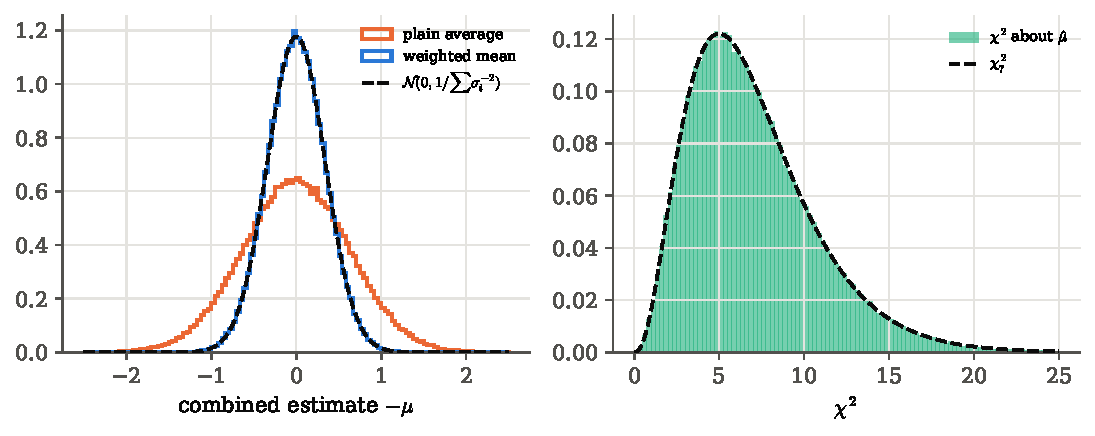
\includegraphics[width=12cm]{figures/ch03/weighted_mean.pdf}
\caption{Left: over many repetitions of the eight-laboratory campaign, the
weighted mean (blue) is a narrow Gaussian of width $W^{-1/2}$ (dashed),
while the plain average (orange) is almost twice as wide. Right: the
histogram of $\chi^2_{\min}$ about the weighted mean lies on the $\chi^2$
curve with $7=N-1$ degrees of freedom, not $8$.}
\label{3a:fig:weighted-mean}
\end{figure}

\subsection{Correlated measurements}
\label{3a:sec:weighted-corr}

Measurements are often correlated. Two analyses may use the same data in
part, the same luminosity, the same energy calibration
(\cref{3a:ex:common-calib}) or the same theory input. Let the measurements
$\bm x=(x_1,\dots,x_N)\T$ be unbiased, $\E x_i=\mu$, with a known covariance
matrix $V$, and write $\bm1=(1,\dots,1)\T$ for the column of ones. The
linear combination $\hat\mu=\bm w\T\bm x$ is still unbiased exactly when
$\bm1\T\bm w=\sum_iw_i=1$ \srcref{Cowan}{(7.31)--(7.32)}, since the
derivation of \eqref{3a:eq:wmean-bias} never used independence. Its
variance is the error-propagation formula \eqref{3a:eq:prop-matrix} with the
$1\times N$ Jacobian $A=\bm w\T$, and this is exact because the map is
linear (\cref{3a:sec:linear-exact}):
\begin{equation}
  \Var\hat\mu=\sum_{i,j}w_iV_{ij}w_j=\bm w\T V\bm w
  \label{3a:eq:wcorr-var}
\end{equation}
\srcref{Cowan}{(7.33)}. We minimise it with a multiplier as before
(Cowan eliminates $w_N$ instead; a multiplier is quicker):
\begin{align}
  \bm0 &\eqby{1} \nabla_{\bm w}\bigl[\bm w\T V\bm w-\lambda(\bm1\T\bm w-1)\bigr]
        \eqby{2} 2V\bm w-\lambda\bm1
  \quad\Longrightarrow\quad \bm w=\frac{\lambda}{2}V^{-1}\bm1,\notag\\
  1 &\eqby{3} \bm1\T\bm w=\frac{\lambda}{2}\,\bm1\T V^{-1}\bm1
  \quad\Longrightarrow\quad \bm w=\frac{V^{-1}\bm1}{\bm1\T V^{-1}\bm1},\notag\\
  \Var\hat\mu &\eqby{4} \frac{\bm1\T V^{-1}\,V\,V^{-1}\bm1}{(\bm1\T V^{-1}\bm1)^2}
  = \frac{1}{\bm1\T V^{-1}\bm1}.
  \label{3a:eq:wcorr-weights}
\end{align}
\begin{explain}
  \item Stationarity in all $w_k$ at once.
  \item $\partial(\bm w\T V\bm w)/\partial w_k=\sum_j(V_{kj}+V_{jk})w_j=2(V\bm w)_k$,
        because $V$ is symmetric.
  \item Impose the constraint to fix $\lambda$.
  \item Insert $\bm w$ into \eqref{3a:eq:wcorr-var}. $V^{-1}$ is symmetric,
        so $\bm w\T=\bm1\T V^{-1}/(\bm1\T V^{-1}\bm1)$, and $V^{-1}VV^{-1}=V^{-1}$.
\end{explain}
In components, $w_i=\sum_j(V^{-1})_{ij}\big/\sum_{k,l}(V^{-1})_{kl}$
\srcref{Cowan}{(7.30)}. For uncorrelated measurements
$(V^{-1})_{ij}=\delta_{ij}/\sigma_i^2$ and we are back at
\eqref{3a:eq:wmean-weights}. The same weights minimise the generalised
$\chi^2(\mu)=(\bm x-\mu\bm1)\T V^{-1}(\bm x-\mu\bm1)$
\srcref{Cowan}{(7.28)}, whose derivative
$-2\bm1\T V^{-1}(\bm x-\mu\bm1)$ vanishes at
$\mu=\bm1\T V^{-1}\bm x/\bm1\T V^{-1}\bm1$. That this least-squares
combination is also the minimum-variance unbiased linear one is an instance
of the Gauss--Markov theorem \srcref{Cowan}{p.~108}.

\paragraph{Two correlated measurements.}
Two measurements already show every new effect of correlation. With
correlation coefficient $\rho$,
\begin{equation}
  V=\begin{pmatrix}\sigma_1^2&\rho\sigma_1\sigma_2\\ \rho\sigma_1\sigma_2&\sigma_2^2\end{pmatrix},
  \qquad
  V^{-1}=\frac{1}{1-\rho^2}
  \begin{pmatrix}\dfrac{1}{\sigma_1^2}&\dfrac{-\rho}{\sigma_1\sigma_2}\\[2mm]
  \dfrac{-\rho}{\sigma_1\sigma_2}&\dfrac{1}{\sigma_2^2}\end{pmatrix}
  \label{3a:eq:wcorr-V2}
\end{equation}
\srcref{Cowan}{(7.34)--(7.35)}. (Check: the inverse of
$\bigl(\begin{smallmatrix}a&b\\b&d\end{smallmatrix}\bigr)$ is
$\bigl(\begin{smallmatrix}d&-b\\-b&a\end{smallmatrix}\bigr)/(ad-b^2)$, and
here $ad-b^2=\sigma_1^2\sigma_2^2(1-\rho^2)$.) Then
\begin{align}
  \bm1\T V^{-1}\bm1
  &\eqby{1}\frac{1}{1-\rho^2}\Bigl[\frac{1}{\sigma_1^2}+\frac{1}{\sigma_2^2}-\frac{2\rho}{\sigma_1\sigma_2}\Bigr]
   \eqby{2}\frac{\sigma_1^2+\sigma_2^2-2\rho\sigma_1\sigma_2}{(1-\rho^2)\sigma_1^2\sigma_2^2},
  \label{3a:eq:wcorr-info2}\\
  w\equiv w_1
  &\eqby{3}\frac{\bigl[1/\sigma_1^2-\rho/(\sigma_1\sigma_2)\bigr]/(1-\rho^2)}{\bm1\T V^{-1}\bm1}
   \eqby{4}\frac{\sigma_2^2-\rho\sigma_1\sigma_2}{\sigma_1^2+\sigma_2^2-2\rho\sigma_1\sigma_2},
  \qquad w_2=1-w,
  \label{3a:eq:wcorr-w2}\\
  \Var\hat\mu
  &\eqby{5}\frac{(1-\rho^2)\sigma_1^2\sigma_2^2}{\sigma_1^2+\sigma_2^2-2\rho\sigma_1\sigma_2}
  \label{3a:eq:wcorr-var2}
\end{align}
\srcref{Cowan}{(7.36)--(7.39)}.
\begin{explain}
  \item The sum of all four entries of $V^{-1}$.
  \item Common denominator $\sigma_1^2\sigma_2^2$.
  \item $(V^{-1}\bm1)_1$ is the sum of the first row of $V^{-1}$.
  \item Multiply numerator and denominator by $(1-\rho^2)\sigma_1^2\sigma_2^2$.
  \item $\Var\hat\mu=1/(\bm1\T V^{-1}\bm1)$ from \eqref{3a:eq:wcorr-weights}
        and \eqref{3a:eq:wcorr-info2}.
\end{explain}

How much does the second measurement help? Subtract the information of the
first alone:
\begin{equation}
  \frac{1}{\Var\hat\mu}-\frac{1}{\sigma_1^2}
  \eqby{1}\frac{1}{1-\rho^2}\Bigl[\frac{1}{\sigma_1^2}+\frac{1}{\sigma_2^2}-\frac{2\rho}{\sigma_1\sigma_2}-\frac{1-\rho^2}{\sigma_1^2}\Bigr]
  \eqby{2}\frac{1}{1-\rho^2}\Bigl[\frac{\rho^2}{\sigma_1^2}-\frac{2\rho}{\sigma_1\sigma_2}+\frac{1}{\sigma_2^2}\Bigr]
  \eqby{3}\frac{1}{1-\rho^2}\Bigl(\frac{\rho}{\sigma_1}-\frac{1}{\sigma_2}\Bigr)^2 .
  \label{3a:eq:wcorr-gain}
\end{equation}
\begin{explain}
  \item \eqref{3a:eq:wcorr-info2}, with $1/\sigma_1^2$ written over the
        same denominator $1-\rho^2$.
  \item $1/\sigma_1^2-(1-\rho^2)/\sigma_1^2=\rho^2/\sigma_1^2$.
  \item The bracket is a perfect square.
\end{explain}
This is never negative \srcref{Cowan}{(7.40)}: a second measurement never
hurts, even a correlated one. The gain is zero exactly when
$\rho=\sigma_1/\sigma_2$, which includes the trivial case of the same
measurement entered twice ($\rho=1$, $\sigma_1=\sigma_2$). And for
$\rho>\sigma_1/\sigma_2$ the weight $w$ of \eqref{3a:eq:wcorr-w2} exceeds
one, so the worse measurement gets a \emph{negative} weight and
$\hat\mu=wx_1+(1-w)x_2$ lies outside the interval between $x_1$ and $x_2$
\srcref{Cowan}{p.~109}.

This is not a paradox. With a strong positive correlation, both measurements
are likely to err in the same direction. If the noisier one reads higher
than the precise one, it is telling us that the common error pushed both up,
the precise one too, so the true value probably lies \emph{below} both. The
optimal combination extrapolates. As $\rho\to1$ the variance
\eqref{3a:eq:wcorr-var2} goes to zero (for $\sigma_1\ne\sigma_2$): the
difference $x_1-x_2$ then measures the common error exactly, and it can be
subtracted.

\paragraph{The same formula cleans the microwave sky.}
A CMB experiment observes the sky in several frequency channels. In the
temperature units used for the CMB, the CMB itself has the same amplitude in
every channel, while the Galactic dust, synchrotron and free--free emission
change strongly with frequency, and every channel has its own noise. So each
channel map is exactly a reading of the form \eqref{3a:eq:hidden-s},
$x_\nu=s+(\text{foregrounds}+\text{noise})_\nu$, at every pixel. Take as
$V$ the covariance of the channel maps measured from the maps themselves,
foregrounds included, and apply \eqref{3a:eq:wcorr-weights}: the weights
$\bm w=V^{-1}\bm1/(\bm1\T V^{-1}\bm1)$ keep the CMB at unit normalisation,
since $\bm1\T\bm w=1$, and minimise everything else together, which is
possible because the foregrounds are strongly correlated between channels,
the large-$\rho$ regime just described, with negative weights doing the
subtracting. This is the \newterm{internal linear combination} (ILC)
\cite{Tegmark2003ILC}. The foregrounds dominate on some angular scales and in
some parts of the sky and not in others, so a single set of weights for the
whole map is a compromise. The needlet ILC, NILC \cite{Delabrouille2009NILC},
splits the maps into pieces localised both in scale and on the sky (needlets)
and computes a separate $V$, hence separate weights, in each piece. It is one
of the four methods behind the Planck maps that \cref{ch:12,ch:13} analyse
\cite{Planck2018IV}. One caveat comes straight from the derivation: the
weights are computed from the same data they are applied to, so the chance
correlation between CMB and foregrounds in a finite patch is partly
subtracted too, which biases the cleaned map slightly low (the ILC bias);
it is small when each piece contains many pixels.

\paragraph{The same thing in Python.}
The second half of \pyname{07_weighted_mean.py} takes $\sigma_1=1$,
$\sigma_2=2$, evaluates \eqref{3a:eq:wcorr-w2} and \eqref{3a:eq:wcorr-var2}
on a grid of $\rho$, and, at seven values of $\rho$, draws $200\,000$
correlated pairs with \pyname{rng.multivariate_normal}, forms
$wx_1+(1-w)x_2$ and measures its variance. \Cref{3a:fig:correlated-combination}
shows the result. At $\rho=0.9$ the simulation gives $\ThreeACorrVmcNine$
against the formula's $\ThreeACorrVthNine$, well below the better
measurement's own variance $\sigma_1^2=1$.

\begin{figure}[htbp]
\centering
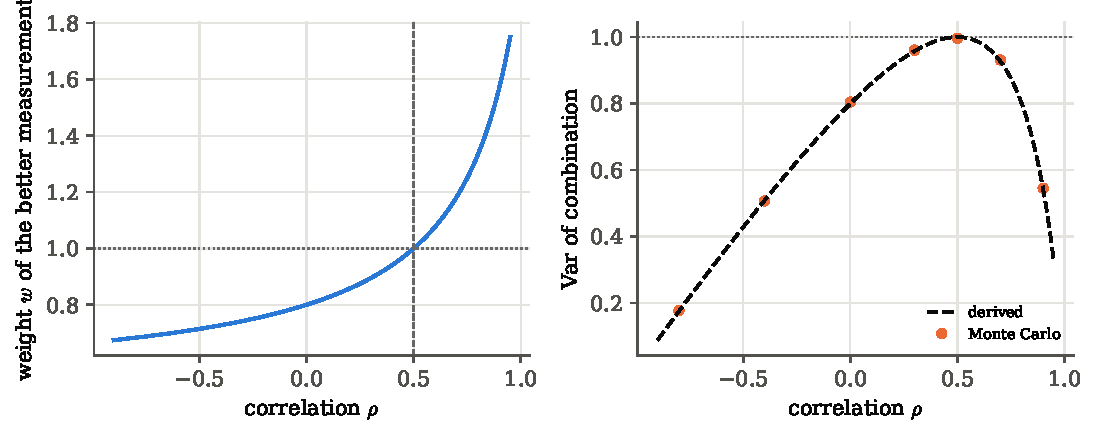
\includegraphics[width=12cm]{figures/ch03/correlated_combination.pdf}
\caption{Combining two measurements with $\sigma_1=1$ and $\sigma_2=2$ as
their correlation $\rho$ varies. Left: the weight of the better measurement
passes $1$ at $\rho=\sigma_1/\sigma_2=0.5$ (dashed vertical line), and
beyond it the poorer measurement is subtracted. Right: the variance of the
optimal combination (dashed curve, formula; dots, simulation) touches the
better measurement's variance $1$ only at $\rho=0.5$ and falls towards zero
as $\rho\to1$.}
\label{3a:fig:correlated-combination}
\end{figure}

\paragraph{Example: two rulers and one thermometer.}
Cowan's example makes the negative weight concrete
\srcref{Cowan}{\S7.6.1}. We measure a length $\lambda$ with two rulers of
different materials, calibrated at temperature $T_0$, with thermal expansion
coefficients $c_1$ and $c_2$. Each reading $L_i$ is corrected with the
measured temperature $T$,
\begin{equation}
  y_i=L_i+c_i(T-T_0),
  \label{3a:eq:rulers}
\end{equation}
\srcref{Cowan}{(7.41)}. The readings have independent errors $\sigma_L$, and
the one thermometer reading $T$ has error $\sigma_T$ and enters both
corrections. Linear propagation, exact here, gives
\begin{align*}
  \sigma_i^2 &\eqby{1} \sigma_L^2+c_i^2\sigma_T^2,\qquad
  V_{12} \eqby{2} c_1c_2\sigma_T^2,\qquad
  \rho\eqby{3}\frac{c_1c_2\sigma_T^2}{\sqrt{(\sigma_L^2+c_1^2\sigma_T^2)(\sigma_L^2+c_2^2\sigma_T^2)}}
\end{align*}
\srcref{Cowan}{(7.42)--(7.44)}.
\begin{explain}
  \item Variance of a sum of independent terms, with
        $\Var[c_i(T-T_0)]=c_i^2\sigma_T^2$.
  \item The only error the two corrected lengths share is the temperature
        error, as in \cref{3a:ex:common-calib}:
        $\Cov(c_1T,c_2T)=c_1c_2\sigma_T^2$.
  \item $\rho=V_{12}/(\sigma_1\sigma_2)$.
\end{explain}
Take $c_1=0.02$ and $c_2=0.05\,\mathrm{mm\,K^{-1}}$, $\sigma_L=0.01\,$mm and
$\sigma_T=2\,$K, and suppose the room is really at $22^\circ$C, two degrees
above $T_0=20^\circ$C, for a true length of $1000.00\,$mm; the thermometer
reads $25^\circ$C. The corrected lengths come out as $y_1=1000.06$ and
$y_2=1000.15\,$mm. The numbers are
\begin{align*}
  \sigma_1^2&=10^{-4}+4\times10^{-4}\times4=0.0017,\qquad
  \sigma_2^2=10^{-4}+25\times10^{-4}\times4=0.0101,\qquad
  V_{12}=0.004,\\
  \rho&=\frac{0.004}{\sqrt{0.0017\times0.0101}}=0.965
  \;>\;\frac{\sigma_1}{\sigma_2}=0.410,\\
  w&\eqby{1}\frac{\sigma_2^2-V_{12}}{\sigma_1^2+\sigma_2^2-2V_{12}}
   =\frac{0.0061}{0.0038}=1.605,\\
  \hat\lambda&\eqby{2}1000+1.605\times0.06-0.605\times0.15=1000.006\,\mathrm{mm},\qquad
  \sigma_{\hat\lambda}\eqby{3}\sqrt{\frac{\sigma_1^2\sigma_2^2-V_{12}^2}{0.0038}}=0.018\,\mathrm{mm}.
\end{align*}
\begin{explain}
  \item \eqref{3a:eq:wcorr-w2} with $\rho\sigma_1\sigma_2=V_{12}$.
  \item $\hat\lambda=wy_1+(1-w)y_2$, written relative to $1000\,$mm.
  \item \eqref{3a:eq:wcorr-var2}, again with $\rho\sigma_1\sigma_2=V_{12}$,
        so that $(1-\rho^2)\sigma_1^2\sigma_2^2=\sigma_1^2\sigma_2^2-V_{12}^2$.
\end{explain}
The combination $1000.006\pm0.018\,$mm lies \emph{outside} the interval
$[1000.06,1000.15]$ and is right, whereas the naive weighted mean that ignores
the correlation gives $1000.073\pm0.038\,$mm, too high by twice its own
error.

Why is a value outside both readings right? \Cref{3a:fig:rulers} shows it.
Each corrected length is a straight line in the unknown true temperature.
Both rulers measure the same length, so they must agree at the true
temperature. The estimate is therefore pulled towards the point where the
two lines cross \srcref{Cowan}{Fig.~7.7}. The same fit returns an estimate of
the temperature itself, $\hat T=22.2^\circ$C, from
\srcref{Cowan}{(7.47)}: the disagreement between the rulers has been used
to correct the thermometer. In the limit $\sigma_L\to0$ ($\rho\to1$) the
two lines give $\hat\lambda=(c_2y_1-c_1y_2)/(c_2-c_1)$ with zero
variance.\footnote{This follows from \eqref{3a:eq:rulers} with exact
readings: then $y_i=\lambda+c_i(T-T_{\text{true}})$, and eliminating
$T-T_{\text{true}}$ between $i=1,2$ gives $c_2y_1-c_1y_2=(c_2-c_1)\lambda$.
Cowan's (7.46) has $c_1$ and $c_2$ interchanged in the numerators; the
check $c_1=0$ (a ruler that does not expand, so $\lambda=y_1$) confirms the
version given here.}

\begin{figure}[htbp]
\centering
\begin{tikzpicture}
\begin{axis}[width=10cm,height=6.2cm,
  xmin=19,xmax=27,ymin=-0.08,ymax=0.2,
  xlabel={assumed true temperature (${}^\circ$C)},
  ylabel={corrected length $-1000$ (mm)},
  tick label style={font=\footnotesize},label style={font=\small},
  yticklabel style={/pgf/number format/fixed},
  scaled y ticks=false,
  legend style={font=\footnotesize,at={(0.02,0.98)},anchor=north west,draw=none,fill=none},
  clip=true]
  \addplot[draw=none,fill=formblue!18,domain=19:27,forget plot] {-0.04+0.02*(x-20)+0.01} \closedcycle;
  \addplot[draw=none,fill=white,domain=19:27,forget plot] {-0.04+0.02*(x-20)-0.01} \closedcycle;
  \addplot[very thick,formblue,domain=19:27] {-0.04+0.02*(x-20)};
  \addlegendentry{ruler 1, $c_1=0.02$}
  \addplot[very thick,fibreorange,domain=19:27] {-0.10+0.05*(x-20)};
  \addlegendentry{ruler 2, $c_2=0.05$}
  \addplot[fibreorange,thin,dashed,domain=19:27,forget plot] {-0.10+0.05*(x-20)+0.01};
  \addplot[fibreorange,thin,dashed,domain=19:27,forget plot] {-0.10+0.05*(x-20)-0.01};
  \draw[softgray,dashed] (axis cs:25,-0.08) -- (axis cs:25,0.2);
  \fill[formblue] (axis cs:25,0.06) circle (2pt);
  \fill[fibreorange] (axis cs:25,0.15) circle (2pt);
  \node[font=\footnotesize,anchor=west] at (axis cs:25.15,0.06) {$y_1$};
  \node[font=\footnotesize,anchor=west] at (axis cs:25.15,0.15) {$y_2$};
  \node[font=\footnotesize,anchor=north,align=center] at (axis cs:25.9,-0.03) {thermometer\\ reads $25^\circ$};
  \fill[bdryred] (axis cs:22.16,0.0055) circle (2.2pt);
  \node[font=\footnotesize,anchor=north west] at (axis cs:22.3,-0.005) {$(\hat T,\hat\lambda)$};
\end{axis}
\end{tikzpicture}
\caption{Two rulers read at a thermometer reading of $25^\circ$C give the
corrected lengths $y_1$ and $y_2$ (dots on the dashed vertical line). If the
temperature were different, each corrected length would slide along its
own line, whose slope is the ruler's expansion coefficient; the shaded
strip and the thin dashed lines show the $\pm\sigma_L$ reading error. Both
rulers measure one length, so the truth sits where the lines cross. The
correlated weighted mean (red dot) lands there, below both $y_1$ and
$y_2$, and at a temperature near $22^\circ$C.}
\label{3a:fig:rulers}
\end{figure}

\paragraph{How research uses it.}
Every world average of a particle mass or lifetime is an inverse-variance
weighted mean, quoted with its $\chi^2_{\min}$ and, when needed, the
inflation factor of \cref{3a:sec:wchi2}. When several experiments share
systematic errors, the correlated formula \eqref{3a:eq:wcorr-weights} is
used under the name ``best linear unbiased estimate'' (the original
discussion is by Lyons and collaborators, \srcref{Cowan}{p.~109}). The hard
part is not the algebra but the off-diagonal elements of $V$, which must be
estimated.

Here our Monte Carlo only \emph{verifies} formulas we derived. In research
the covariance of the inputs is itself often taken from simulations, and
then its noise (\cref{3a:sec:cov-noise}) passes into the weights.

In cosmology the same algebra appears in a more general form. Combining
independent probes with Gaussian likelihoods multiplies the likelihoods,
and multiplying Gaussians adds their inverse covariances. For one parameter that is
exactly $1/\sigma^2=\sum_i1/\sigma_i^2$; for many parameters it is the
statement that Fisher matrices add (\cref{ch:10}).

\paragraph{Where this leaves us.}
Every error bar so far came from one idea: treat a summary of the data as a
random variable over imagined repetitions, and ask for its centre and width.
The weighted mean showed a second way of seeing the same numbers. The
density of the data, read as a function of the unknown $\mu$, peaked at the
estimator and had a width equal to its standard error. That reading of the
density is the likelihood, the subject of the second half of the chapter.
Maximising it gives estimators, and its curvature gives their error bars.

\begin{recap}[Part 3a in one page]
\begin{itemize}
  \item An estimator $\hat\theta=g(x_1,\dots,x_N)$ is a random variable. Its
        sampling distribution over imagined repetitions gives the error bar
        (the standard error). Simulate it when in doubt.
  \item $\mathrm{MSE}=\mathrm{bias}^2+\mathrm{variance}$. Consistency:
        $\hat\theta\to\theta$ in probability, guaranteed when bias and
        variance both go to zero.
  \item $\Var\bar x=\sigma^2/N$: errors shrink like $1/\sqrt N$ (law of
        large numbers via Chebyshev). The central limit theorem makes the
        sampling distribution of a mean Gaussian.
  \item $S^2$ divides by $N-1$ to be unbiased. Its own error is
        $\Var S^2=2\sigma^4/(N-1)$ for Gaussian data (cosmic variance is the
        same fact).
  \item Sample covariance and correlation matrices are noisy: sample
        correlations of independent variables scatter by $\sim1/\sqrt N$,
        and inverting a simulated covariance needs the Hartlap factor.
  \item Error propagation: $U=AVA\T$ with the Jacobian $A$, exact for linear
        maps. It fails near poles and for noisy denominators; use Monte Carlo
        propagation there.
  \item Combining measurements: weight by $1/\sigma_i^2$, so
        $1/\sigma_{\hat\mu}^2=\sum_i1/\sigma_i^2$. Check
        $\chi^2_{\min}\sim\chi^2_{N-1}$. With correlations,
        $\bm w=V^{-1}\bm1/(\bm1\T V^{-1}\bm1)$, and weights can be negative.
\end{itemize}
\end{recap}

\providecommand{\ThreeBBernArea}{}\renewcommand{\ThreeBBernArea}{3.780\times10^{-7}}
\providecommand{\ThreeBBernAreaNum}{}\renewcommand{\ThreeBBernAreaNum}{3.780\times10^{-7}}
\providecommand{\ThreeBBernLmax}{}\renewcommand{\ThreeBBernLmax}{1.427\times10^{-6}}
\providecommand{\ThreeBBernRatio}{}\renewcommand{\ThreeBBernRatio}{0.265}
\providecommand{\ThreeBUnifMax}{}\renewcommand{\ThreeBUnifMax}{0.9072}
\providecommand{\ThreeBLifeT}{}\renewcommand{\ThreeBLifeT}{10.51}
\providecommand{\ThreeBAreaTau}{}\renewcommand{\ThreeBAreaTau}{4.920\times10^{-4}}
\providecommand{\ThreeBAreaTauNum}{}\renewcommand{\ThreeBAreaTauNum}{4.920\times10^{-4}}
\providecommand{\ThreeBAreaLam}{}\renewcommand{\ThreeBAreaLam}{8.910\times10^{-5}}
\providecommand{\ThreeBAreaRatio}{}\renewcommand{\ThreeBAreaRatio}{5.522}
\providecommand{\ThreeBDecN}{}\renewcommand{\ThreeBDecN}{50}
\providecommand{\ThreeBDecTauHat}{}\renewcommand{\ThreeBDecTauHat}{0.8831}
\providecommand{\ThreeBDecTauNum}{}\renewcommand{\ThreeBDecTauNum}{0.8831}
\providecommand{\ThreeBDecSigCurv}{}\renewcommand{\ThreeBDecSigCurv}{0.1249}
\providecommand{\ThreeBDecLo}{}\renewcommand{\ThreeBDecLo}{0.114}
\providecommand{\ThreeBDecHi}{}\renewcommand{\ThreeBDecHi}{0.1376}
\providecommand{\ThreeBDecSdTh}{}\renewcommand{\ThreeBDecSdTh}{0.1414}
\providecommand{\ThreeBDecSdMC}{}\renewcommand{\ThreeBDecSdMC}{0.1406}
\providecommand{\ThreeBDecMeanTau}{}\renewcommand{\ThreeBDecMeanTau}{1.003}
\providecommand{\ThreeBDecMeanCurv}{}\renewcommand{\ThreeBDecMeanCurv}{0.1419}
\providecommand{\ThreeBDecCoverCurv}{}\renewcommand{\ThreeBDecCoverCurv}{0.6913}
\providecommand{\ThreeBDecCoverDl}{}\renewcommand{\ThreeBDecCoverDl}{0.6866}
\providecommand{\ThreeBDecLamMean}{}\renewcommand{\ThreeBDecLamMean}{1.017}
\providecommand{\ThreeBDecLamTh}{}\renewcommand{\ThreeBDecLamTh}{1.02}
\providecommand{\ThreeBAngMomA}{}\renewcommand{\ThreeBAngMomA}{0.49}
\providecommand{\ThreeBAngMomB}{}\renewcommand{\ThreeBAngMomB}{0.4458}
\providecommand{\ThreeBAngA}{}\renewcommand{\ThreeBAngA}{0.4885}
\providecommand{\ThreeBAngB}{}\renewcommand{\ThreeBAngB}{0.4396}
\providecommand{\ThreeBAngSa}{}\renewcommand{\ThreeBAngSa}{0.05099}
\providecommand{\ThreeBAngSb}{}\renewcommand{\ThreeBAngSb}{0.107}
\providecommand{\ThreeBAngRho}{}\renewcommand{\ThreeBAngRho}{0.4237}
\providecommand{\ThreeBAngIter}{}\renewcommand{\ThreeBAngIter}{4}
\providecommand{\ThreeBAngStepOneA}{}\renewcommand{\ThreeBAngStepOneA}{0.4885}
\providecommand{\ThreeBAngStepOneB}{}\renewcommand{\ThreeBAngStepOneB}{0.4396}
\providecommand{\ThreeBAngSdA}{}\renewcommand{\ThreeBAngSdA}{0.05376}
\providecommand{\ThreeBAngSdB}{}\renewcommand{\ThreeBAngSdB}{0.1081}
\providecommand{\ThreeBAngRhoMC}{}\renewcommand{\ThreeBAngRhoMC}{0.4919}
\providecommand{\ThreeBAngMomSdA}{}\renewcommand{\ThreeBAngMomSdA}{0.05422}
\providecommand{\ThreeBAngMomSdB}{}\renewcommand{\ThreeBAngMomSdB}{0.1109}
\providecommand{\ThreeBAngMeanA}{}\renewcommand{\ThreeBAngMeanA}{0.502}
\providecommand{\ThreeBAngMeanB}{}\renewcommand{\ThreeBAngMeanB}{0.4986}
\providecommand{\ThreeBAngRhoMCErr}{}\renewcommand{\ThreeBAngRhoMCErr}{0.0339}
\providecommand{\ThreeBAngRhoHessMean}{}\renewcommand{\ThreeBAngRhoHessMean}{0.4263}
\providecommand{\ThreeBAngRhoHessSd}{}\renewcommand{\ThreeBAngRhoHessSd}{0.03868}
\providecommand{\ThreeBAngMomRatioA}{}\renewcommand{\ThreeBAngMomRatioA}{1.009}
\providecommand{\ThreeBAngMomRatioAErr}{}\renewcommand{\ThreeBAngMomRatioAErr}{0.007096}
\providecommand{\ThreeBAngMomRatioB}{}\renewcommand{\ThreeBAngMomRatioB}{1.026}
\providecommand{\ThreeBAngMomRatioBErr}{}\renewcommand{\ThreeBAngMomRatioBErr}{0.009865}
\providecommand{\ThreeBLineA}{}\renewcommand{\ThreeBLineA}{1.238}
\providecommand{\ThreeBLineB}{}\renewcommand{\ThreeBLineB}{0.4187}
\providecommand{\ThreeBLineSa}{}\renewcommand{\ThreeBLineSa}{0.4113}
\providecommand{\ThreeBLineSb}{}\renewcommand{\ThreeBLineSb}{0.08767}
\providecommand{\ThreeBLineRho}{}\renewcommand{\ThreeBLineRho}{-0.8223}
\providecommand{\ThreeBLineChi}{}\renewcommand{\ThreeBLineChi}{11.01}
\providecommand{\ThreeBLineP}{}\renewcommand{\ThreeBLineP}{0.2012}
\providecommand{\ThreeBLineSaMC}{}\renewcommand{\ThreeBLineSaMC}{0.4067}
\providecommand{\ThreeBLineSbMC}{}\renewcommand{\ThreeBLineSbMC}{0.08717}
\providecommand{\ThreeBLineRhoMC}{}\renewcommand{\ThreeBLineRhoMC}{-0.8182}
\providecommand{\ThreeBLineChiMean}{}\renewcommand{\ThreeBLineChiMean}{7.932}
\providecommand{\ThreeBLineChiVar}{}\renewcommand{\ThreeBLineChiVar}{15.69}
\providecommand{\ThreeBLineWrongMean}{}\renewcommand{\ThreeBLineWrongMean}{41.36}
\providecommand{\ThreeBCorrMeanBd}{}\renewcommand{\ThreeBCorrMeanBd}{0.4986}
\providecommand{\ThreeBCorrMeanBf}{}\renewcommand{\ThreeBCorrMeanBf}{0.4994}
\providecommand{\ThreeBCorrQuoted}{}\renewcommand{\ThreeBCorrQuoted}{0.08767}
\providecommand{\ThreeBCorrTrueD}{}\renewcommand{\ThreeBCorrTrueD}{0.1284}
\providecommand{\ThreeBCorrSdD}{}\renewcommand{\ThreeBCorrSdD}{0.1282}
\providecommand{\ThreeBCorrSdF}{}\renewcommand{\ThreeBCorrSdF}{0.1212}
\providecommand{\ThreeBCorrQuotedF}{}\renewcommand{\ThreeBCorrQuotedF}{0.121}
\providecommand{\ThreeBCorrChiD}{}\renewcommand{\ThreeBCorrChiD}{4.77}
\providecommand{\ThreeBCorrChiF}{}\renewcommand{\ThreeBCorrChiF}{8.069}
\providecommand{\ThreeBPoisNobs}{}\renewcommand{\ThreeBPoisNobs}{122}
\providecommand{\ThreeBPoisNuP}{}\renewcommand{\ThreeBPoisNuP}{122}
\providecommand{\ThreeBPoisNuN}{}\renewcommand{\ThreeBPoisNuN}{110.7}
\providecommand{\ThreeBPoisNuS}{}\renewcommand{\ThreeBPoisNuS}{129}
\providecommand{\ThreeBPoisTauP}{}\renewcommand{\ThreeBPoisTauP}{1.076}
\providecommand{\ThreeBPoisTauN}{}\renewcommand{\ThreeBPoisTauN}{0.9253}
\providecommand{\ThreeBPoisTauS}{}\renewcommand{\ThreeBPoisTauS}{1.18}
\providecommand{\ThreeBPoisChiN}{}\renewcommand{\ThreeBPoisChiN}{13.7}
\providecommand{\ThreeBPoisChiS}{}\renewcommand{\ThreeBPoisChiS}{14.01}
\providecommand{\ThreeBPoisBC}{}\renewcommand{\ThreeBPoisBC}{18.47}
\providecommand{\ThreeBPoisZeroBins}{}\renewcommand{\ThreeBPoisZeroBins}{4}
\providecommand{\ThreeBPoisDiffP}{}\renewcommand{\ThreeBPoisDiffP}{3.996\times10^{-9}}
\providecommand{\ThreeBPoisDiffN}{}\renewcommand{\ThreeBPoisDiffN}{-11.65}
\providecommand{\ThreeBPoisDiffS}{}\renewcommand{\ThreeBPoisDiffS}{7.883}
\providecommand{\ThreeBPoisPredN}{}\renewcommand{\ThreeBPoisPredN}{-13.73}
\providecommand{\ThreeBPoisPredS}{}\renewcommand{\ThreeBPoisPredS}{7.883}
\providecommand{\ThreeBPoisTauMeanP}{}\renewcommand{\ThreeBPoisTauMeanP}{1.002}
\providecommand{\ThreeBPoisTauMeanN}{}\renewcommand{\ThreeBPoisTauMeanN}{0.8992}
\providecommand{\ThreeBPoisTauMeanS}{}\renewcommand{\ThreeBPoisTauMeanS}{1.114}
\providecommand{\ThreeBPoisBCmean}{}\renewcommand{\ThreeBPoisBCmean}{18.73}
\providecommand{\ThreeBPoisDof}{}\renewcommand{\ThreeBPoisDof}{18}
\providecommand{\ThreeBEffMeanBig}{}\renewcommand{\ThreeBEffMeanBig}{0.9981}
\providecommand{\ThreeBEffMedBig}{}\renewcommand{\ThreeBEffMedBig}{1.578}
\providecommand{\ThreeBEffNBig}{}\renewcommand{\ThreeBEffNBig}{201}
\providecommand{\ThreeBEffARE}{}\renewcommand{\ThreeBEffARE}{0.6327}
\providecommand{\ThreeBEffAREth}{}\renewcommand{\ThreeBEffAREth}{0.6366}
\providecommand{\ThreeBEffUnifFifty}{}\renewcommand{\ThreeBEffUnifFifty}{0.01877}
\providecommand{\ThreeBEffUnifFiftyTh}{}\renewcommand{\ThreeBEffUnifFiftyTh}{0.01887}
\providecommand{\ThreeBEffNFifty}{}\renewcommand{\ThreeBEffNFifty}{51}
\providecommand{\ThreeBConsTen}{}\renewcommand{\ThreeBConsTen}{1.47}
\providecommand{\ThreeBConsHund}{}\renewcommand{\ThreeBConsHund}{1.031}
\providecommand{\ThreeBConsThou}{}\renewcommand{\ThreeBConsThou}{1.016}
\providecommand{\ThreeBProfNon}{}\renewcommand{\ThreeBProfNon}{20}
\providecommand{\ThreeBProfNoff}{}\renewcommand{\ThreeBProfNoff}{8}
\providecommand{\ThreeBProfK}{}\renewcommand{\ThreeBProfK}{1}
\providecommand{\ThreeBProfS}{}\renewcommand{\ThreeBProfS}{12}
\providecommand{\ThreeBProfB}{}\renewcommand{\ThreeBProfB}{8}
\providecommand{\ThreeBProfLo}{}\renewcommand{\ThreeBProfLo}{5.192}
\providecommand{\ThreeBProfHi}{}\renewcommand{\ThreeBProfHi}{5.47}
\providecommand{\ThreeBCondLo}{}\renewcommand{\ThreeBCondLo}{4.145}
\providecommand{\ThreeBCondHi}{}\renewcommand{\ThreeBCondHi}{4.811}
\providecommand{\ThreeBProfGauss}{}\renewcommand{\ThreeBProfGauss}{5.292}
\providecommand{\ThreeBCondGauss}{}\renewcommand{\ThreeBCondGauss}{4.472}
\providecommand{\ThreeBProfCover}{}\renewcommand{\ThreeBProfCover}{0.6849}
\providecommand{\ThreeBCondCover}{}\renewcommand{\ThreeBCondCover}{0.6088}
\providecommand{\ThreeBProfUsed}{}\renewcommand{\ThreeBProfUsed}{9995}
\providecommand{\ThreeBBootRelOne}{}\renewcommand{\ThreeBBootRelOne}{0.1365}
\providecommand{\ThreeBBootRelMean}{}\renewcommand{\ThreeBBootRelMean}{0.1375}
\providecommand{\ThreeBBootRelSd}{}\renewcommand{\ThreeBBootRelSd}{0.01819}
\providecommand{\ThreeBBootTauHat}{}\renewcommand{\ThreeBBootTauHat}{0.8176}
\providecommand{\ThreeBBootMed}{}\renewcommand{\ThreeBBootMed}{0.5147}
\providecommand{\ThreeBBootSeTauTrue}{}\renewcommand{\ThreeBBootSeTauTrue}{0.1425}
\providecommand{\ThreeBBootSeTauNP}{}\renewcommand{\ThreeBBootSeTauNP}{0.1116}
\providecommand{\ThreeBBootSeTauP}{}\renewcommand{\ThreeBBootSeTauP}{0.1162}
\providecommand{\ThreeBBootSeTauCurv}{}\renewcommand{\ThreeBBootSeTauCurv}{0.1156}
\providecommand{\ThreeBBootSeMedTrue}{}\renewcommand{\ThreeBBootSeMedTrue}{0.1418}
\providecommand{\ThreeBBootSeMedNP}{}\renewcommand{\ThreeBBootSeMedNP}{0.1352}
\providecommand{\ThreeBBootSeMedP}{}\renewcommand{\ThreeBBootSeMedP}{0.1155}
\providecommand{\ThreeBBootNormLo}{}\renewcommand{\ThreeBBootNormLo}{0.2496}
\providecommand{\ThreeBBootNormHi}{}\renewcommand{\ThreeBBootNormHi}{0.7798}
\providecommand{\ThreeBBootPivLo}{}\renewcommand{\ThreeBBootPivLo}{0.1678}
\providecommand{\ThreeBBootPivHi}{}\renewcommand{\ThreeBBootPivHi}{0.6632}
\providecommand{\ThreeBBootPctLo}{}\renewcommand{\ThreeBBootPctLo}{0.3661}
\providecommand{\ThreeBBootPctHi}{}\renewcommand{\ThreeBBootPctHi}{0.8616}
\providecommand{\ThreeBBootMedTrueVal}{}\renewcommand{\ThreeBBootMedTrueVal}{0.6931}
\providecommand{\ThreeBBootFrac}{}\renewcommand{\ThreeBBootFrac}{0.6386}
\providecommand{\ThreeBBootFracTh}{}\renewcommand{\ThreeBBootFracTh}{0.6358}
\providecommand{\ThreeBBootB}{}\renewcommand{\ThreeBBootB}{10000}
\providecommand{\ThreeBRBTruth}{}\renewcommand{\ThreeBRBTruth}{0.2231}
\providecommand{\ThreeBRBCrudeMean}{}\renewcommand{\ThreeBRBCrudeMean}{0.2232}
\providecommand{\ThreeBRBCrudeVar}{}\renewcommand{\ThreeBRBCrudeVar}{0.1734}
\providecommand{\ThreeBRBRBMean}{}\renewcommand{\ThreeBRBRBMean}{0.2231}
\providecommand{\ThreeBRBRBVar}{}\renewcommand{\ThreeBRBRBVar}{0.00799}
\providecommand{\ThreeBRBRatio}{}\renewcommand{\ThreeBRBRatio}{0.04608}
\providecommand{\ThreeBRBCR}{}\renewcommand{\ThreeBRBCR}{0.007468}
\providecommand{\ThreeBRBCrudeVarTh}{}\renewcommand{\ThreeBRBCrudeVarTh}{0.1733}
\providecommand{\ThreeBRBRBVarTh}{}\renewcommand{\ThreeBRBRBVarTh}{0.008057}
\providecommand{\ThreeBRBn}{}\renewcommand{\ThreeBRBn}{10}
\providecommand{\ThreeBRBlam}{}\renewcommand{\ThreeBRBlam}{1.5}
\providecommand{\ThreeBBayesSqArg}{}\renewcommand{\ThreeBBayesSqArg}{3.005}
\providecommand{\ThreeBBayesAbsArg}{}\renewcommand{\ThreeBBayesAbsArg}{2.677}
\providecommand{\ThreeBBayesZOArg}{}\renewcommand{\ThreeBBayesZOArg}{2}
\providecommand{\ThreeBBayesMean}{}\renewcommand{\ThreeBBayesMean}{3}
\providecommand{\ThreeBBayesMedian}{}\renewcommand{\ThreeBBayesMedian}{2.672}
\providecommand{\ThreeBBayesMode}{}\renewcommand{\ThreeBBayesMode}{2}
\providecommand{\ThreeBCMBMeanTwo}{}\renewcommand{\ThreeBCMBMeanTwo}{0.9962}
\providecommand{\ThreeBCMBVarTwo}{}\renewcommand{\ThreeBCMBVarTwo}{0.401}
\providecommand{\ThreeBCMBBoundTwo}{}\renewcommand{\ThreeBCMBBoundTwo}{0.4}
\providecommand{\ThreeBCMBRelErrTwo}{}\renewcommand{\ThreeBCMBRelErrTwo}{0.6332}
\providecommand{\ThreeBCMBMeanThirty}{}\renewcommand{\ThreeBCMBMeanThirty}{1.002}
\providecommand{\ThreeBCMBVarThirty}{}\renewcommand{\ThreeBCMBVarThirty}{0.03236}
\providecommand{\ThreeBCMBBoundThirty}{}\renewcommand{\ThreeBCMBBoundThirty}{0.03279}
\providecommand{\ThreeBCMBRelErrThirty}{}\renewcommand{\ThreeBCMBRelErrThirty}{0.1799}
\providecommand{\ThreeBCMBScoreVarThirty}{}\renewcommand{\ThreeBCMBScoreVarThirty}{30.16}
\providecommand{\ThreeBCMBFishThirty}{}\renewcommand{\ThreeBCMBFishThirty}{30.5}
\providecommand{\ThreeBCMBScoreMeanThirty}{}\renewcommand{\ThreeBCMBScoreMeanThirty}{0.008949}
 
\section{The likelihood: data are the model plus noise}
\label{3b:sec:likelihood}

We measure a voltage, count photons in a detector, record the arrival
times of decays, or estimate a power spectrum from a map of the sky. In every
case we also have a theory with a knob on it: a resistance, a cross-section,
a lifetime, a cosmological parameter. Set the knob to a value $\theta$ and
the theory predicts what the apparatus should have shown. Call that
prediction $d(\theta)$. The apparatus never shows exactly $d(\theta)$. It
shows the prediction plus whatever the noise happened to be on that day.
Until now the question has run one way: \emph{given} the truth, how does a
summary of the data scatter when the experiment is repeated? Now the data
are in, and we ask the opposite question: which values of the knob could
have produced the data we actually have?

The tool for this backward question is the \newterm{likelihood}. It is not a
new probability distribution. It is the old one, the distribution of the
data, read in the other direction. To understand it we need answers to four
questions.
\begin{enumerate}[label=\arabic*.]
  \item How does a model of the noise turn into a number attached to each
        value of $\theta$?
  \item What happens with many measurements?
  \item Why is that number \emph{not} a probability distribution for
        $\theta$, even though it is built from one?
  \item Where does it sit in Bayes' theorem, and what information in the
        data does it keep?
\end{enumerate}
The pipeline of \cref{ch:00} ends with an arrow from how a statistic $S$
scatters, $P(S\given\theta)$, to what the observed value of $S$ says about
the physics. The likelihood is that arrow. It is the sampling distribution
of the data (or of a summary $S$ of them), evaluated at the data we
observed and read as a function of the physics $\theta$.

\subsection{One measurement: from the noise to the likelihood}
\label{3b:sec:one-measurement}

Start with the simplest experiment there is. The model predicts a number
$d(\theta)$, and the measurement adds noise:
\begin{equation}
  D = d(\theta) + \epsilon,\qquad \epsilon\sim\Normal(0,\sigma^2),
  \label{3b:eq:model-noise}
\end{equation}
with $\sigma$ known from calibrating the instrument. The noise $\epsilon$
\unpack{the random amount by which this particular reading differs from the
ideal, noiseless one} has density
$\phi_\sigma(\epsilon)=(2\pi\sigma^2)^{-1/2}\exp(-\epsilon^2/2\sigma^2)$.
What is the density of the reading $D$ itself? Fix $\theta$ and ask for the
probability that $D$ lands in a small window $[D_0,D_0+\dd D]$:
\begin{align}
  \Prob\bigl(D_0\le D\le D_0+\dd D\given\theta\bigr)
  &\eqby{1} \Prob\bigl(D_0-d(\theta)\le \epsilon\le D_0-d(\theta)+\dd D\bigr)
  \nonumber\\
  &\eqby{2} \phi_\sigma\bigl(D_0-d(\theta)\bigr)\,\dd D
  \nonumber\\
  &\eqby{3} \frac{1}{\sqrt{2\pi\sigma^2}}
     \exp\!\left[-\frac{\bigl(D_0-d(\theta)\bigr)^2}{2\sigma^2}\right]\dd D .
  \label{3b:eq:one-point}
\end{align}
\begin{explain}
  \item At fixed $\theta$ the prediction $d(\theta)$ is just a number, so
        $D=d(\theta)+\epsilon$ lies in the window exactly when $\epsilon$
        lies in the same window shifted down by $d(\theta)$.
  \item For a small window, probability is density times width. A shift does
        not stretch the window, so the width is still $\dd D$.
  \item Insert the Gaussian density of the noise.
\end{explain}
So $D\sim\Normal(d(\theta),\sigma^2)$: the reading is Gaussian, centred on
the prediction, with the width of the noise. Nothing new so far. This is the
\emph{forward} or \emph{prediction} direction: fix the physics, ask how the
data would scatter.

Now the data are in. We hold $D=D_0$ fixed at the value on the lab book and
let $\theta$ vary instead. The same expression becomes a function of $\theta$,
\begin{equation}
  \Like(\theta)\equiv p(D_0\given\theta)
  =\frac{1}{\sqrt{2\pi\sigma^2}}
   \exp\!\left[-\frac{\bigl(D_0-d(\theta)\bigr)^2}{2\sigma^2}\right]
  =\phi_\sigma\bigl(\underbrace{D_0-d(\theta)}_{\text{required noise}}\bigr).
  \label{3b:eq:like-one}
\end{equation}
The last form says what the likelihood measures. Take a trial value
$\theta$. The model predicts $d(\theta)$. To turn that prediction into the
reading we actually got, the noise must have been exactly
$\epsilon=D_0-d(\theta)$. The likelihood is the probability density of
\emph{that} noise value. So for each trial $\theta$ it answers one question:
how probable is the noise that this $\theta$ needs in order to explain our
reading?

\begin{keyidea}[what the likelihood measures]
Pick a trial value $\theta$. The model then says what the reading should have
been, $d(\theta)$, and the gap $D_0-d(\theta)$ is the noise that nature would
have had to add to turn that prediction into the reading we actually got. The
likelihood of $\theta$ is how probable this particular piece of noise is.
In symbols it is nothing more than the distribution of the data: if
$D=d(\theta)+\epsilon$ with $\epsilon\sim\Normal(0,1)$, then
$D\sim\Normal(d(\theta),1)$, and this density, with $D$ held at the observed
value and $\theta$ left free, is the likelihood function. For noise of width
$\sigma$, as in \eqref{3b:eq:like-one}, the $1$ becomes $\sigma^2$.
\end{keyidea}

A value of $\theta$ whose prediction sits close to the data needs only a
small, ordinary fluctuation and gets a high likelihood. A value whose
prediction sits five noise widths away needs a five-sigma fluctuation and
gets a likelihood smaller by a factor $e^{-25/2}\approx4\times10^{-6}$.
\Cref{3b:fig:residual-gaussians} draws exactly this for several data
points and two trial models.

In the language of the backward question, each trial value of $\theta$ is a
candidate explanation, the reading $D_0$ is what we saw, and the likelihood
ranks the candidates by how easily each one would have produced that reading.
Parameter estimation in \cref{ch:05} is built on exactly this.

\begin{figure}[htbp]
\centering
\begin{tikzpicture}[x=0.95cm,y=1.05cm]
  \foreach \panel/\xs/\a/\b/\name in {0/0/1.0/0.5/{\theta_A},1/6.6/2.45/0.0/{\theta_B}}{
  \begin{scope}[xshift=\xs cm]
    \draw[->,faint] (0,0.3) -- (5.9,0.3) node[below left,font=\footnotesize,black] {$x$};
    \draw[->,faint] (0,0.3) -- (0,4.9) node[left,font=\footnotesize,black] {$D$};
    \draw[form] (0.2,{\a+\b*0.2}) -- (5.7,{\a+\b*5.7});
    \node[font=\footnotesize,formblue,anchor=west] at (0.15,4.6) {model $d(x;\name)$};
    \foreach \xi/\yi in {1/1.6,2/1.9,3/2.7,4/2.9,5/3.6}{
      \pgfmathsetmacro{\m}{\a+\b*\xi}
      \draw[fibre,thin,smooth,samples=41,domain={\m-1.25}:{\m+1.25},variable=\y]
        plot ({\xi+0.62*exp(-((\y-\m)^2)/(2*0.09))},\y);
      \draw[faint,densely dotted] (\xi,{\m-1.25}) -- (\xi,{\m+1.25});
      \draw[bdry,thick] (\xi,\m) -- (\xi,\yi);
      \draw[tangentgreen,thick] (\xi,\yi) -- ({\xi+0.62*exp(-((\yi-\m)^2)/(2*0.09))},\yi);
      \fill[black] (\xi,\yi) circle (1.6pt);
    }
  \end{scope}}
  \node[font=\footnotesize,align=center] at (3.0,-0.25) {$\theta_A$: small residuals,\\ every datum near the peak};
  \node[font=\footnotesize,align=center] at (9.6,-0.25) {$\theta_B$: large residuals,\\ data far out in the tails};
\end{tikzpicture}
\caption{The likelihood of two trial parameter values. Black dots are the
same five measurements in both panels. The blue line is the model prediction
for the trial value, and the orange curve on its side at each $x$ is the
noise density $\Normal(d,\sigma^2)$ centred on the prediction. The red
segment is the fluctuation the noise would have had to produce, and the
length of the green tick is the height of the noise density at the datum.
The likelihood is the product of the five green lengths. On the left they
are all long. On the right two of them are almost zero, so $\theta_B$ needs
an implausible noise realisation.}
\label{3b:fig:residual-gaussians}
\end{figure}

\begin{workdef}[likelihood]
For data $\data$ and a model that gives the data a probability
(or density) $p(\data\given\params)$ for each parameter value, the
\newterm{likelihood} is that same function with the data held fixed at
their observed values and the parameters varied,
\[
  \Like(\params)\equiv p(\data_{\text{obs}}\given\params).
\]
\emph{Operationally:} write down the noise model that turns a prediction
$d(\params)$ into data \unpack{for example ``add independent Gaussian noise of
known width''}, compute the probability of the observed data under it, and
treat the answer as a function of $\params$ alone. The
\newterm{log-likelihood} is $\ell(\params)=\ln\Like(\params)$.
\end{workdef}

\paragraph{Example: one reading of a resistance.}
We pass a known current $I=2\,$A through a resistor and read the voltage
with a voltmeter whose noise is $\sigma=0.2\,$V. The model is Ohm's law,
$d(R)=IR$, and the reading is $D_0=10.4\,$V. Then
\begin{align*}
  \Like(R)
  &\eqby{1}\frac{1}{\sqrt{2\pi}\,(0.2\,\mathrm V)}
     \exp\!\left[-\frac{(10.4\,\mathrm V-2\,\mathrm A\cdot R)^2}{2(0.2\,\mathrm V)^2}\right]\\
  &\eqby{2}\frac{1}{\sqrt{2\pi}\,(0.2\,\mathrm V)}
     \exp\!\left[-\frac{(R-5.2\,\Omega)^2}{2(0.1\,\Omega)^2}\right].
\end{align*}
\begin{explain}
  \item \eqref{3b:eq:like-one} with $d(R)=IR$.
  \item Factor $I^2$ out of the square:
        $(D_0-IR)^2=I^2(R-D_0/I)^2$, and $\sigma^2/I^2=(0.1\,\Omega)^2$.
\end{explain}
As a function of $R$ the likelihood is a Gaussian bump centred at
$5.2\,\Omega$ with width $0.1\,\Omega$. The peak is at the resistance whose
prediction needs zero noise: $IR=D_0$ gives $R=10.4\,\mathrm V/2\,\mathrm
A=5.2\,\Omega$. The width is the noise width divided by the slope
$\dd d/\dd R=I$, because a change $\delta R$ moves the prediction by
$I\,\delta R$. The prefactor carries units of $\mathrm{V}^{-1}$, because it
is a density in the \emph{voltage}, not in $R$. That is the first sign that
the likelihood is not a probability density for $R$
(\cref{3b:sec:not-density}).

\subsection{Many measurements: the product and the logarithm}
\label{3b:sec:product}

Real experiments have many data points $D_1,\dots,D_N$, taken at settings
$x_1,\dots,x_N$, with predictions $d_i(\theta)=d(x_i;\theta)$. If the noise
in different readings is independent, the joint density factorises, because
independence means precisely that the joint density is the product of the
single ones \srcref{Sivia}{p.~65, (3.62)}:
\begin{align}
  \Like(\theta)
  &\eqby{1} p(D_1,\dots,D_N\given\theta)
   \eqby{2} \prod_{i=1}^N p(D_i\given\theta)
  \nonumber\\
  &\eqby{3} \prod_{i=1}^N\frac{1}{\sqrt{2\pi\sigma_i^2}}
     \exp\!\left[-\frac{\bigl(D_i-d_i(\theta)\bigr)^2}{2\sigma_i^2}\right],
  \label{3b:eq:like-product}\\
  \ell(\theta)
  &\eqby{4} -\frac12\sum_{i=1}^N\frac{\bigl(D_i-d_i(\theta)\bigr)^2}{\sigma_i^2}
   \;-\;\sum_{i=1}^N\ln\sqrt{2\pi\sigma_i^2} .
  \label{3b:eq:loglike-gauss}
\end{align}
\begin{explain}
  \item Definition of the likelihood for the whole data vector.
  \item Independent noise: the probability of the joint noise realisation
        is the product of the probabilities of the individual ones.
  \item Insert \eqref{3b:eq:one-point} for each reading, with its own
        noise width $\sigma_i$.
  \item The logarithm of a product is the sum of the logarithms, and
        $\ln e^{u}=u$.
\end{explain}
The first sum in \eqref{3b:eq:loglike-gauss} is
$\chi^2(\theta)$: each residual $D_i-d_i(\theta)$ is divided by its error
bar $\sigma_i$, squared, and the squares are added. The second sum does not
depend on $\theta$ at all. So, for Gaussian noise,
$\ell(\theta)=-\tfrac12\chi^2(\theta)+\text{const}$. This is why least
squares works (\cref{3b:sec:least-squares}).

For identically distributed data, $x_1,\dots,x_n$ drawn independently from
one density $f(x;\theta)$, the same steps give Wasserman's definition
\mainref{p.~122, Def.~9.7},
\begin{equation}
  \Like_n(\theta)=\prod_{i=1}^n f(x_i;\theta),\qquad
  \ell_n(\theta)=\sum_{i=1}^n\ln f(x_i;\theta).
  \label{3b:eq:like-iid}
\end{equation}
Three practical remarks follow from the product structure.
\begin{enumerate}[label=(\roman*)]
  \item \emph{Work with logarithms.} A product of a thousand densities of
        size $0.1$ is $10^{-1000}$ and underflows every computer. Its
        logarithm, $-2303$, is harmless. Sums are also what we
        differentiate most easily.
  \item \emph{Constants do not matter.} Multiplying $\Like$ by any positive
        number $c$ that does not depend on $\theta$ changes nothing we will
        do with it: the location of the maximum, the shape, and ratios
        $\Like(\theta_1)/\Like(\theta_2)$ are all unchanged
        \mainref{p.~123, Remark~9.9}. We drop such constants freely and write
        $\Like\propto\dots$.
  \item \emph{Only ratios carry meaning.} Since the overall constant is
        arbitrary, the statement ``$\Like(\theta_1)=0.03$'' means nothing.
        The statement ``$\Like(\theta_1)/\Like(\theta_2)=20$'' means that the
        data are twenty times more probable under $\theta_1$ than under
        $\theta_2$. The cosmology literature often reports
        $-2\ln[\Like(\theta)/\Like_{\max}]$ \srcref{Padilla}{(26)}, which is
        a $\Delta\chi^2$ for Gaussian noise.
\end{enumerate}

\paragraph{Example: a coin, or any yes/no detector.}
A detector fires ($x_i=1$) or not ($x_i=0$) with unknown probability $p$.
Each trial is Bernoulli, $f(x;p)=p^x(1-p)^{1-x}$. In $n=20$ trials it
fires $S=\sum_ix_i=12$ times \mainref{p.~123, Ex.~9.10}. Then
\begin{align*}
  \Like(p)
  &\eqby{1}\prod_{i=1}^{n}p^{x_i}(1-p)^{1-x_i}
   \eqby{2}p^{\sum_ix_i}(1-p)^{n-\sum_ix_i}
   = p^{12}(1-p)^{8}.
\end{align*}
\begin{explain}
  \item \eqref{3b:eq:like-iid} with the Bernoulli probability.
  \item Collect the powers: $\prod_ip^{x_i}=p^{\sum_ix_i}$ and likewise for
        $1-p$.
\end{explain}
The left panel of \cref{3b:fig:likelihood-shapes} shows it. It is a smooth
bump with its peak at $p=S/n=0.6$. The individual zeros and ones have
disappeared: only their sum $S$ enters.

\paragraph{Example: a uniform distribution with an unknown end point.}
Let $x_i\sim\mathrm{Uniform}(0,\theta)$, with density $1/\theta$ on
$[0,\theta]$ and zero outside \mainref{p.~124, Ex.~9.12}. Each factor of
the product is $1/\theta$ if $x_i\le\theta$ and zero if $x_i>\theta$. The
product is nonzero only if \emph{every} $x_i\le\theta$, that is, if
$\theta\ge x_{(n)}\equiv\max_ix_i$:
\[
  \Like(\theta)=
  \begin{cases}
    \theta^{-n}, & \theta\ge x_{(n)},\\
    0,           & \theta< x_{(n)}.
  \end{cases}
\]
A value $\theta$ smaller than the largest observation is not merely
implausible, it is impossible: no noise realisation can put a point above the
end of the box. For ten simulated points with largest value
$x_{(10)}=\ThreeBUnifMax$, the middle panel of
\cref{3b:fig:likelihood-shapes} shows a cliff at $x_{(10)}$ followed by a
decay as $\theta^{-10}$. It has no smooth peak. Because of that cliff, this
model breaks rules that smooth likelihoods obey: the maximum is not found by
setting a derivative to zero (\cref{3b:sec:mle-hand}), and the Cram\'er--Rao
bound does not apply (\cref{3b:sec:cramer-rao}).

\subsection{The likelihood is not a probability density for \texorpdfstring{$\theta$}{theta}}
\label{3b:sec:not-density}

The likelihood is not the probability density of $\theta$. The temptation is
real: it is built from a density, and in the resistor example it even looked
like a Gaussian in $R$. Two facts show that it is not a density for
$\theta$. Its area over $\theta$ is arbitrary, and it does not change the way a
density must when we rename the parameter.

\paragraph{The area under the likelihood is arbitrary.}
Integrate the resistor likelihood over $R$:
\begin{align*}
  \int_{-\infty}^{\infty}\Like(R)\,\dd R
  &\eqby{1}\frac{1}{\sqrt{2\pi}\,\sigma}\int_{-\infty}^{\infty}
     \exp\!\left[-\frac{(R-D_0/I)^2}{2(\sigma/I)^2}\right]\dd R
   \eqby{2}\frac{1}{\sqrt{2\pi}\,\sigma}\sqrt{2\pi}\,\frac{\sigma}{I}
   =\frac1I = 0.5\,\mathrm{A}^{-1}.
\end{align*}
\begin{explain}
  \item The form found in the resistor example, with $\sigma=0.2\,$V.
  \item The Gaussian integral
        $\int e^{-(u-u_0)^2/2s^2}\dd u=\sqrt{2\pi}\,s$ with $s=\sigma/I$.
\end{explain}
If $\Like(R)$ were a probability density for $R$, this area would be $1$.
It is $0.5$, and it is not even a pure number: it has units of inverse
amperes. Change the current to $1\,$A and the area becomes $1$. Measure the
current in milliamperes and it changes again. The reason is that the
likelihood is a density in the \emph{data}: it integrates to one over $D$,
by construction, and its units are those of $1/D$. Nothing fixes its
integral over $\theta$.

The same happens in every example. For the detector,
\begin{align*}
  \int_0^1\Like(p)\,\dd p
  \eqby{1}\int_0^1p^{S}(1-p)^{n-S}\,\dd p
  \eqby{2}B(S+1,n-S+1)
  \eqby{3}\frac{S!\,(n-S)!}{(n+1)!}
  =\frac{12!\,8!}{21!}=\ThreeBBernArea ,
\end{align*}
\begin{explain}
  \item The Bernoulli likelihood of the example above.
  \item The Beta integral $\int_0^1p^{a-1}(1-p)^{b-1}\dd p=B(a,b)$, the
        normalising constant of the Beta distribution (\cref{ch:02}), with
        $a=S+1$, $b=n-S+1$.
  \item $B(a,b)=\Gamma(a)\Gamma(b)/\Gamma(a+b)$ and $\Gamma(m+1)=m!$.
\end{explain}
and the numerical integral in \pyname{08_likelihood_shapes.py} gives the
same number, $\ThreeBBernAreaNum$. The peak value is
$\Like(0.6)=\ThreeBBernLmax$, so the area is only $\ThreeBBernRatio$ times
the peak height (in units of $p$). Nothing about it is one.

\paragraph{Renaming the parameter changes the area but not the values.}
The second fact goes deeper. When we change the name of the parameter, a
density picks up a Jacobian factor and the likelihood does not. To see it,
take $k=5$ decay times with total $T=\sum_it_i=\ThreeBLifeT$ (in units of
the true lifetime), and describe the decay either by the mean life $\tau$ or
by the rate $\lambda=1/\tau$. With $f(t;\tau)=\tau^{-1}e^{-t/\tau}$,
\begin{align*}
  \Like(\tau)&\eqby{1}\prod_{i=1}^k\frac1\tau e^{-t_i/\tau}
   =\tau^{-k}e^{-T/\tau},
  &\int_0^\infty\Like(\tau)\,\dd\tau
   &\eqby{2}\frac{\Gamma(k-1)}{T^{k-1}}=\ThreeBAreaTau,\\
  \Like(\lambda)&\eqby{3}\prod_{i=1}^k\lambda e^{-\lambda t_i}
   =\lambda^{k}e^{-\lambda T},
  &\int_0^\infty\Like(\lambda)\,\dd\lambda
   &\eqby{4}\frac{\Gamma(k+1)}{T^{k+1}}=\ThreeBAreaLam .
\end{align*}
\begin{explain}
  \item \eqref{3b:eq:like-iid} with the exponential density.
  \item Substitute $u=T/\tau$, $\dd\tau=-T\,\dd u/u^2$:
        $\int_0^\infty\tau^{-k}e^{-T/\tau}\dd\tau
        =T^{1-k}\int_0^\infty u^{k-2}e^{-u}\dd u=T^{1-k}\Gamma(k-1)$.
  \item The same density written with $\lambda$: $f(t;\lambda)=\lambda e^{-\lambda t}$.
  \item The Gamma integral $\int_0^\infty\lambda^ke^{-\lambda T}\dd\lambda
        =\Gamma(k+1)/T^{k+1}$.
\end{explain}
The two areas differ by a factor $T^2/[k(k-1)]=\ThreeBAreaRatio$. Yet at
corresponding points the two functions are \emph{equal}: putting
$\lambda=1/\tau$ into $\lambda^ke^{-\lambda T}$ gives
$\tau^{-k}e^{-T/\tau}$, so $\Like(\lambda=1/\tau)=\Like(\tau)$. The
likelihood behaves like a scalar field. It assigns a number to each physical
hypothesis (``the lifetime is $1.3\,$ns''), whatever coordinate we use to
name that hypothesis.

A genuine probability density behaves differently. If $p_\tau(\tau)$ were a
density for $\tau$, the probability of a small interval $\dd\tau$ would be
$p_\tau\,\dd\tau$. The same interval written in $\lambda$ has width
$\dd\lambda=\dd\tau/\tau^2$, and the probability must be the same, so the
density for $\lambda$ would be
$p_\lambda(\lambda)=p_\tau(1/\lambda)\,|\dd\tau/\dd\lambda|
=p_\tau(1/\lambda)/\lambda^2$. The factor $1/\lambda^2$ is the Jacobian. The
likelihood never picks one up, so the areas under it in different
coordinates disagree, and neither area means anything. The right panel of
\cref{3b:fig:likelihood-shapes} shows the two curves, each scaled to peak
height one: the same heights at corresponding points, but different shapes
along the axis.

\begin{figure}[htbp]
\centering
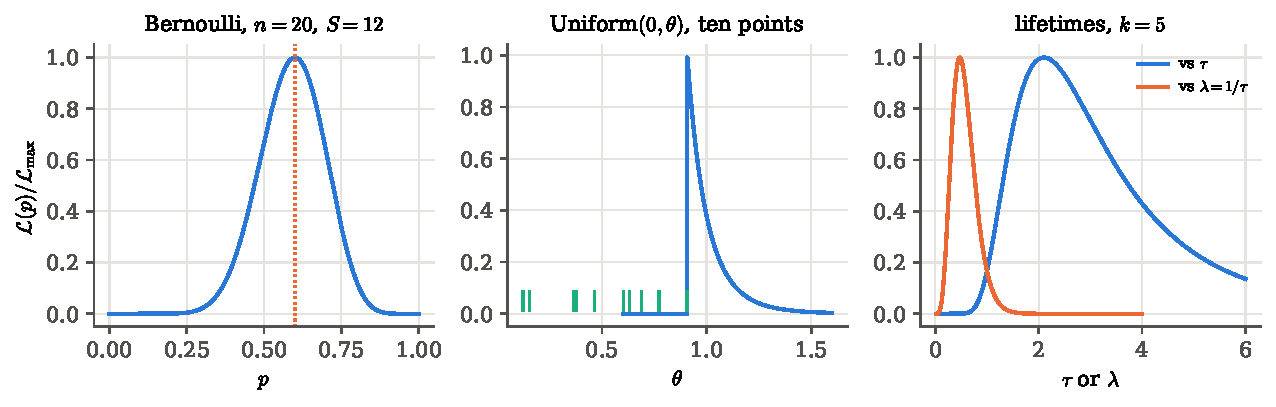
\includegraphics[width=12cm]{figures/ch03/likelihood_shapes.pdf}
\caption{Three likelihoods, each scaled to a maximum of one. Left: a
yes/no detector that fired 12 times in 20 trials, a smooth bump peaked at
$p=0.6$. Middle: ten points from a uniform box of unknown length (ticks
at the bottom). The likelihood is zero until $\theta$ reaches the largest
point, then decays as $\theta^{-10}$. Right: five decay times, with the
likelihood drawn once against the mean life $\tau$ and once against the rate
$\lambda=1/\tau$. The two curves take the same value at $\lambda=1/\tau$,
but they enclose different areas.}
\label{3b:fig:likelihood-shapes}
\end{figure}

\begin{keyidea}[The likelihood is a function of $\theta$, not a distribution over $\theta$]
$\Like(\theta)=p(\data_{\text{obs}}\given\theta)$ is normalised over the
\emph{data}, $\int p(\data\given\theta)\,\dd\data=1$ for every $\theta$. Over
$\theta$ it has no normalisation, it changes no Jacobian under a change of
parameter, and only ratios $\Like(\theta_1)/\Like(\theta_2)$ are meaningful
\mainref{p.~122}. To get a probability distribution over $\theta$ one needs
a prior, and Bayes' theorem (\cref{ch:05}).
\end{keyidea}

\subsection{Prediction and inference: where the likelihood sits}
\label{3b:sec:bayes-place}

The two readings of $p(\data\given\theta)$ are the two directions of
probability that run through the whole book (\cref{ch:01}). Read forward, it
starts from a fixed $\theta$ and says which data sets that $\theta$ can
produce, and how often. Read backward, the data set is already in hand, and
we ask which values of $\theta$ could have produced it and how much each one
deserves to be believed now that we have it.

\emph{Prediction} is the first reading, \emph{inference} the second.
\Cref{3b:fig:two-directions} draws both as trees. In the prediction
tree one parameter value fans out into many possible data sets, and their
probabilities add to one. In the inference tree many parameter values point
at the one data set we have, and the numbers attached to the branches are the
likelihoods. They need not add to anything.

So, facing data, we ask two questions in words before writing anything.
First: which values of $\theta$ could have produced these data? Second: how
probable would these data have been under each of them? The answers to the
second question, read across all $\theta$, are the likelihood. The first
question fixes what the posterior will be a distribution over. Turning the
likelihood into that distribution needs one more ingredient, a prior
(\cref{ch:05}).

\begin{figure}[htbp]
\centering
\begin{tikzpicture}[
  pt/.style={draw=accent,thick,rounded corners=2pt,fill=ideabg,font=\small,
             minimum height=7mm,minimum width=14mm,align=center},
  obs/.style={pt,draw=fibreorange!80!black,fill=defbg},
  flow/.style={->,thick,accent}]
  \node[pt] (th) at (0,0) {$\theta$ fixed};
  \node[pt] (d1) at (3.0,1.2) {$\data^{(1)}$};
  \node[pt] (d2) at (3.0,0) {$\data^{(2)}$};
  \node[pt] (d3) at (3.0,-1.2) {$\data^{(3)}$};
  \foreach \k in {1,2,3} \draw[flow] (th) -- (d\k);
  \node[font=\footnotesize,align=center] at (2.2,-2.3)
       {$p(\data^{(k)}\given\theta)$\\ add up to $1$};
  \node[font=\small\bfseries,accent] at (1.6,2.1) {prediction};
  \node[pt] (t1) at (8.2,1.2) {$\theta_1$};
  \node[pt] (t2) at (8.2,0) {$\theta_2$};
  \node[pt] (t3) at (8.2,-1.2) {$\theta_3$};
  \node[obs] (dobs) at (11.0,0) {$\data_{\text{obs}}$};
  \foreach \k in {1,2,3} \draw[flow] (t\k) -- (dobs);
  \node[font=\footnotesize,align=center] at (9.6,-2.3)
       {$\Like(\theta_k)=p(\data_{\text{obs}}\given\theta_k)$\\ need not add to $1$};
  \node[font=\small\bfseries,accent] at (9.6,2.1) {inference};
\end{tikzpicture}
\caption{The same conditional probability read two ways. Left: one
hypothesis produces many possible data sets, and the probabilities of all of
them sum to one. Right: many hypotheses could have produced the single data
set we observed (orange). The likelihood attaches to each hypothesis the
probability that it would have produced exactly these data. These numbers
compare hypotheses with each other but are not a distribution over them.}
\label{3b:fig:two-directions}
\end{figure}

Bayes' theorem is the bridge from one tree to the other. Written for
parameters it reads \srcref{HobsonBMC}{p.~11, (1.25)}
\begin{equation}
  \underbrace{p(\theta)}_{\text{prior}}\;
  \underbrace{p(\data\given\theta)}_{\text{likelihood}}
  \;=\;p(\theta,\data)\;=\;
  \underbrace{p(\data)}_{\text{evidence }Z}\;
  \underbrace{p(\theta\given\data)}_{\text{posterior}} .
  \label{3b:eq:bayes}
\end{equation}
Both sides are the joint probability of parameter and data, $p(\theta,\data)$,
split into two factors in the two possible orders. The likelihood is the
part the experiment supplies. It is also the least controversial part. We
can calibrate the instrument with known inputs and count how often it
produces each output, which pins $p(\data\given\theta)$ down to any desired
precision \srcref{HobsonBMC}{p.~11}. The prior, the evidence and the
posterior belong to \cref{ch:05}. Two facts about them are needed now.
First, with a flat prior $p(\theta)=\text{const}$ the posterior is
proportional to the likelihood, so the peak of the posterior is the peak of
the likelihood \srcref{Sivia}{p.~64, (3.61)}. Second, ``flat'' depends on
the parametrisation. A prior flat in $\tau$ is not flat in $\lambda=1/\tau$,
because of the Jacobian $1/\lambda^2$ found above. From here on we stay
on the frequentist side and use the likelihood by itself, without any prior.

\paragraph{What the likelihood keeps: sufficiency.}
In each of the three examples the likelihood depended on the data through
one number only: the count $S$ of detector firings, the total decay time
$T$, and the largest value $x_{(n)}$ of the uniform box. Two detector data
sets with the same $S$ give the same likelihood function, so nothing
computed from the likelihood can tell them apart. A statistic with this
property is called \newterm{sufficient}
\unpack{knowing its value lets us write down the whole likelihood function,
up to a constant factor} \mainref{p.~137, Def.~9.32}. The factorisation
theorem \mainref{p.~140, Thm.~9.40} gives a quick test: $T(\data)$ is
sufficient exactly when $p(\data\given\theta)=g\bigl(T(\data),\theta\bigr)\,h(\data)$.
For Gaussian data with unknown $\mu$ and $\sigma$ the pair
$(\bar x,S^2)$ is sufficient \mainref{p.~138, Ex.~9.34}: the likelihood
$\propto\sigma^{-n}\exp\{-[(n-1)S^2+n(\bar x-\mu)^2]/2\sigma^2\}$ uses
nothing else. Cosmologists use the same compression every day: when a map
is Gaussian and statistically isotropic, its power spectrum carries all the
information about the parameters. Sufficiency also improves estimators. The
Rao--Blackwell
theorem says that averaging any estimator over all data sets that share
the observed value of a sufficient statistic gives a new estimator whose
mean squared error is never larger \mainref{p.~140, Thm.~9.42}: an
estimator that uses anything beyond the sufficient statistic is only
adding noise.

\paragraph{The likelihood principle.}
The \newterm{likelihood principle} goes one step further
\srcref{CasellaBerger}{\S6.3.1}. It says that if two data sets $\data$ and
$\data'$ give proportional likelihoods, $\Like(\theta\given\data)=
c\,\Like(\theta\given\data')$ for all $\theta$, then they carry the same
evidence about $\theta$ and should lead to the same conclusion. Two coin
experiments show what this means. Experimenter A decides to toss a coin
$n=20$ times and sees $S=12$ heads. The count is binomial, and
$\Like\propto p^{12}(1-p)^8$. Experimenter B decides to toss until the
eighth tail, and the eighth tail comes on toss $20$, so B also saw $12$
heads and $8$ tails. That count is negative binomial, and again
$\Like\propto p^{12}(1-p)^8$, only with a different constant in front. The
likelihoods are proportional, so by the principle A and B have learned the
same thing about $p$. Estimates and intervals built from the likelihood
alone respect the principle. Procedures that average over data sets that could have been
observed but were not, such as $p$-values (\cref{ch:04}), depend on the
stopping rule, so they violate it. Bayesian inference satisfies it
automatically, because the posterior uses the data only through
$\Like(\theta)$ \srcref{CasellaBerger}{\S6.3.2}.
\section{Maximum likelihood: pick the value that needs the least unusual noise}
\label{3b:sec:mle}

The likelihood $\Like(\theta)$ of \cref{3b:sec:likelihood} gives every
candidate value of $\theta$ a number: how readily that value would have
produced the data we hold. If we must report a single value, the natural
choice is the one with the highest number. Its prediction needs the most
ordinary noise to become the data. This is the
\newterm{maximum likelihood estimator}, and it is the workhorse of
experimental physics. Almost every fitted mass, lifetime, cross-section and
cosmological parameter you have seen was obtained this way, or by its
Gaussian special case, least squares.

Turning the idea into recipes raises three questions.
\begin{enumerate}[label=\arabic*.]
  \item How do we find the maximum when we can do the calculus by hand, and
        what do the answers look like for the standard models?
  \item How does it compare with the older recipe of matching moments?
  \item How do we find the maximum when we cannot do the calculus, and how
        does that look in Python?
\end{enumerate}
The recipe is worth using because, for large samples, it homes in on the
truth, is nearly unbiased, and is as precise as any estimator can be. These
properties are proved in \cref{3b:sec:properties}. Its error bar comes from
the width of the likelihood (\cref{3b:sec:curvature}).

\begin{workdef}[maximum likelihood estimator]
The \newterm{maximum likelihood estimator} (MLE) $\hat\theta$ is the value of
$\theta$ that maximises $\Like(\theta)$, or equivalently
$\ell(\theta)=\ln\Like(\theta)$ \mainref{p.~122, Def.~9.8}. When the maximum
is inside the allowed range and $\ell$ is smooth, it solves the
\newterm{score equation}
\[
  S(\theta)\equiv\frac{\partial\ell}{\partial\theta}=0,
  \qquad \frac{\partial^2\ell}{\partial\theta^2}<0 ,
\]
where the \newterm{score} $S(\theta)$ \unpack{the slope of the
log-likelihood, a random quantity because it depends on the data} measures
how much the data pull $\theta$ up or down. For several parameters every
component of the gradient vanishes and the matrix of second derivatives is
negative definite.
\end{workdef}

Before differentiating we may throw away every factor of $\Like$ that does
not contain $\theta$. Two facts allow it. First, $\ln$ is increasing, so
$\Like$ and $\ell$ peak at the same $\theta$. Second, a constant factor in
$\Like$ becomes an added constant in $\ell$, and the derivative of a
constant is zero.

\subsection{Solving the score equation by hand}
\label{3b:sec:mle-hand}

\paragraph{Example: the mean lifetime of an unstable particle.}
We record $n$ decay times $t_1,\dots,t_n$ from $f(t;\tau)=\tau^{-1}e^{-t/\tau}$
\srcref{Cowan}{\S6.2}. Then
\begin{align}
  \ell(\tau)&\eqby{1}\sum_{i=1}^n\Bigl(-\ln\tau-\frac{t_i}{\tau}\Bigr)
             =-n\ln\tau-\frac{T}{\tau},\qquad T\equiv\sum_it_i,
  \nonumber\\
  S(\tau)&\eqby{2}-\frac n\tau+\frac{T}{\tau^2}
          \eqby{3}0
  \quad\Longrightarrow\quad
  \hat\tau=\frac Tn=\bar t,
  \label{3b:eq:tau-mle}\\
  \ell''(\hat\tau)&\eqby{4}\frac{n}{\hat\tau^2}-\frac{2T}{\hat\tau^3}
   \eqby{5}-\frac{n}{\hat\tau^2}<0 .
  \nonumber
\end{align}
\begin{explain}
  \item Logarithm of the product \eqref{3b:eq:like-iid}:
        $\ln(\tau^{-1}e^{-t/\tau})=-\ln\tau-t/\tau$.
  \item Differentiate term by term: $\dd(-n\ln\tau)/\dd\tau=-n/\tau$ and
        $\dd(-T/\tau)/\dd\tau=T/\tau^2$.
  \item The score equation. Multiply by $\tau^2$ to get $-n\tau+T=0$.
  \item Differentiate once more: $\dd(-n/\tau)/\dd\tau=n/\tau^2$,
        $\dd(T/\tau^2)/\dd\tau=-2T/\tau^3$.
  \item At $\hat\tau$ we have $T=n\hat\tau$, so $2T/\hat\tau^3=2n/\hat\tau^2$.
\end{explain}
The maximum likelihood lifetime is the average decay time. It is unbiased,
$\E\bar t=\tau$, and its variance is $\tau^2/n$, because the exponential has
variance $\tau^2$ and averaging $n$ independent times divides the variance
by $n$. This is the same estimator whose sampling distribution we simulated
for the muon lifetime in \cref{3a:ex:lifetime}. The number
$-\ell''(\hat\tau)=n/\hat\tau^2$ is one over the square of the error bar, as
\cref{3b:sec:curvature} shows.

\paragraph{Example: the centre and width of a Gaussian.}
Let $x_i\sim\Normal(\mu,\sigma^2)$ with both parameters unknown
\mainref{p.~123, Ex.~9.11}, \srcref{Cowan}{\S6.3},
\srcref{CasellaBerger}{Ex.~7.2.11}. Dropping the constant $-\tfrac n2\ln2\pi$,
\begin{align*}
  \ell(\mu,\sigma)&\eqby{1}-n\ln\sigma-\frac{1}{2\sigma^2}\sum_{i=1}^n(x_i-\mu)^2,\\
  \frac{\partial\ell}{\partial\mu}&\eqby{2}\frac1{\sigma^2}\sum_i(x_i-\mu)=0
  \;\Longrightarrow\;\hat\mu=\bar x,\\
  \frac{\partial\ell}{\partial\sigma}&\eqby{3}-\frac n\sigma+\frac1{\sigma^3}\sum_i(x_i-\mu)^2=0
  \;\Longrightarrow\;\hat\sigma^2=\frac1n\sum_i(x_i-\bar x)^2 .
\end{align*}
\begin{explain}
  \item $\ln$ of $\prod_i(2\pi\sigma^2)^{-1/2}e^{-(x_i-\mu)^2/2\sigma^2}$,
        with $\ln(\sigma^2)^{-n/2}=-n\ln\sigma$.
  \item The chain rule on $(x_i-\mu)^2$ gives $-2(x_i-\mu)$. The sum
        vanishes when $n\mu=\sum_ix_i$.
  \item Differentiate $-n\ln\sigma$ and $\sigma^{-2}$; multiply the equation
        by $\sigma^3/n$; and insert the solution $\mu=\bar x$ of the first
        equation, because both equations must hold at once.
\end{explain}
The centre is the sample mean, as one would guess. The width divides by
$n$, not $n-1$, and so it is \emph{biased}. In \cref{3a:sec:n-minus-one} we
showed that $\E\sum_i(x_i-\bar x)^2=(n-1)\sigma^2$. Dividing by $n$ gives
$\E\hat\sigma^2=\tfrac{n-1}{n}\sigma^2$: the MLE is low by a factor
$(n-1)/n$. The bias is the price of estimating $\mu$ from the same data, and
it vanishes as $n\to\infty$. Maximum likelihood promises good behaviour for
large samples, not unbiasedness at every $n$.

\paragraph{Example: the firing probability of a detector.}
For the Bernoulli likelihood $p^S(1-p)^{n-S}$ of \cref{3b:sec:product},
\[
  \ell(p)=S\ln p+(n-S)\ln(1-p),\qquad
  S(p)=\frac Sp-\frac{n-S}{1-p}=0
  \;\Longrightarrow\;\hat p=\frac Sn ,
\]
because multiplying the score equation by $p(1-p)$ gives
$S(1-p)-(n-S)p=S-np=0$. For $S=12$ in $n=20$ trials, $\hat p=0.6$, the peak
seen in \cref{3b:fig:likelihood-shapes}.

\paragraph{Example: when the maximum sits on an edge.}
For the uniform box the likelihood $\theta^{-n}$ decreases for all
$\theta\ge x_{(n)}$ and is zero below, so the maximum is at the cliff,
$\hat\theta=x_{(n)}$ \mainref{p.~124}. The score equation
$-n/\theta=0$ has no solution at all; the maximum is found by looking, not
by differentiating. The estimator is biased low, because the largest of $n$
points always falls short of the end of the box:
$\E x_{(n)}=\tfrac{n}{n+1}\theta$. A related case arises whenever physics
restricts the parameter. A signal strength $\mu$ cannot be negative. If we
measure $x_i\sim\Normal(\mu,\sigma^2)$ and find $\bar x<0$, the likelihood
restricted to $\mu\ge0$ is largest at the edge, so $\hat\mu=0$
\srcref{CasellaBerger}{Ex.~7.2.8}. The derivative there is not zero, and
several of the nice properties of \cref{3b:sec:properties} fail at such
boundaries.

\begin{pitfall}[The MLE is not ``the most probable value of $\theta$'']
$\hat\theta$ is the value under which the \emph{data} are most probable. It
is the most probable value of $\theta$ only in a Bayesian analysis with a
flat prior, and then only in the parametrisation in which the prior is flat
\srcref{Sivia}{p.~64}. Because the likelihood carries no Jacobian, the
MLE itself does not care about the parametrisation:
$\hat\lambda=1/\hat\tau$ (\cref{3b:sec:properties}). The peak of a posterior
\emph{density} does move under a change of variables.
\end{pitfall}

\subsection{The method of moments, for comparison}
\label{3b:sec:mom}

Before maximum likelihood there was a simpler idea. A model with $k$
parameters predicts the first $k$ moments $\alpha_j(\theta)=\E_\theta X^j$
\unpack{the average of the $j$-th power of the data, as a function of the
parameters}. The data give the sample moments
$\hat\alpha_j=\tfrac1n\sum_ix_i^j$. The \newterm{method of moments}
estimator sets the two equal and solves,
$\alpha_j(\tilde\theta)=\hat\alpha_j$ for $j=1,\dots,k$
\mainref{p.~121, Def.~9.3}, \srcref{Cowan}{Ch.~8}. For the Bernoulli
model, $\E X=p$ gives $\tilde p=\bar x=S/n$; for the Gaussian, $\E X=\mu$
and $\E X^2=\sigma^2+\mu^2$ give $\tilde\mu=\bar x$ and
$\tilde\sigma^2=\tfrac1n\sum x_i^2-\bar x^2=\tfrac1n\sum(x_i-\bar x)^2$
\mainref{p.~121, Exs.~9.4--9.5}. Both coincide with the MLE. Under mild
conditions the moment estimator is consistent and asymptotically Gaussian
\mainref{p.~122, Thm.~9.6}, but in general it throws information away, and
the MLE is at least as precise for large samples (\cref{3b:sec:properties}).

\paragraph{Example: an angular distribution.}
In $e^+e^-\to\mu^+\mu^-$ the distribution of $x=\cos\theta$ of the outgoing
muon has the shape $1+\alpha x+\beta x^2$, where $\beta$ comes from the
photon exchange and $\alpha$, the forward--backward asymmetry, from its
interference with the $Z$. The detector accepts only
$x_{\min}\le x\le x_{\max}$, so the density is
\srcref{Cowan}{\S6.8, (8.9)}
\begin{equation}
  f(x;\alpha,\beta)=\frac{1+\alpha x+\beta x^2}{d_1+\alpha d_2+\beta d_3},
  \qquad d_k\equiv\frac{x_{\max}^k-x_{\min}^k}{k},
  \label{3b:eq:angular}
\end{equation}
because
$\int_{x_{\min}}^{x_{\max}}(1+\alpha x+\beta x^2)\,\dd x=d_1+\alpha d_2+\beta d_3$.
The first two moments are ratios of the same kind,
\begin{align*}
  \E x&\eqby{1}\frac{d_2+\alpha d_3+\beta d_4}{d_1+\alpha d_2+\beta d_3},&
  \E x^2&\eqby{2}\frac{d_3+\alpha d_4+\beta d_5}{d_1+\alpha d_2+\beta d_3},
\end{align*}
\begin{explain}
  \item $\int x(1+\alpha x+\beta x^2)\,\dd x=d_2+\alpha d_3+\beta d_4$.
  \item $\int x^2(1+\alpha x+\beta x^2)\,\dd x=d_3+\alpha d_4+\beta d_5$.
\end{explain}
and setting them equal to $\hat\alpha_1=\overline{x}$ and
$\hat\alpha_2=\overline{x^2}$ and multiplying out gives two \emph{linear}
equations for $(\alpha,\beta)$,
\[
  \alpha(\hat\alpha_1d_2-d_3)+\beta(\hat\alpha_1d_3-d_4)=d_2-\hat\alpha_1d_1,
  \qquad
  \alpha(\hat\alpha_2d_2-d_4)+\beta(\hat\alpha_2d_3-d_5)=d_3-\hat\alpha_2d_1 .
\]
For $2000$ simulated events with $\alpha=\beta=0.5$ on
$-0.95\le x\le0.95$ (Cowan's set-up), these give
$(\tilde\alpha,\tilde\beta)=(\ThreeBAngMomA,\ThreeBAngMomB)$. The maximum
likelihood equations for the same model are not linear, so they need a
numerical method.

\subsection{When the calculus cannot be done: Newton--Raphson}
\label{3b:sec:newton}

For \eqref{3b:eq:angular} the log-likelihood is
$\ell(\alpha,\beta)=\sum_i\ln(1+\alpha x_i+\beta x_i^2)-n\ln(d_1+\alpha d_2+\beta d_3)$,
and its score equations have no closed-form solution. The standard
numerical maximiser replaces $\ell$ near a trial point by a parabola and
jumps to the parabola's top. The same parabola gives the error bar in
\cref{3b:sec:curvature}. Near a trial point $\theta_j$,
\begin{align}
  \ell(\theta)&\eqby{1}\ell(\theta_j)+\ell'(\theta_j)(\theta-\theta_j)
   +\tfrac12\ell''(\theta_j)(\theta-\theta_j)^2+\dots,
  \nonumber\\
  0&\eqby{2}\ell'(\theta_j)+\ell''(\theta_j)(\theta_{j+1}-\theta_j)
  \quad\Longrightarrow\quad
  \theta_{j+1}=\theta_j-\frac{\ell'(\theta_j)}{\ell''(\theta_j)} .
  \label{3b:eq:newton}
\end{align}
\begin{explain}
  \item Taylor expansion to second order: we replace $\ell$ by the parabola
        that has the same value, slope and curvature at $\theta_j$.
  \item Jump to the top of that parabola, where its derivative vanishes.
\end{explain}
With several parameters, $\ell'$ becomes the gradient $\bm g$ and $\ell''$
the matrix of second derivatives $H$ (the \newterm{Hessian}), and the step
is $\params_{j+1}=\params_j-H^{-1}\bm g$. Near the maximum the error shrinks
quadratically, roughly squaring at every step, so a handful of iterations
suffice. \Cref{3b:fig:newton} shows the first two steps on a lifetime
likelihood.

\paragraph{Example: Newton by hand.}
Take $n=5$ decays with total time $T=6$, so that $\ell(\tau)=-5\ln\tau-6/\tau$,
$\ell'=-5/\tau+6/\tau^2$, $\ell''=5/\tau^2-12/\tau^3$, and the exact answer
is $\hat\tau=T/n=1.2$. Start at $\tau_0=0.8$:
\begin{align*}
  \tau_1&\eqby{1}0.8-\frac{-6.25+9.375}{7.8125-23.4375}
        =0.8+\frac{3.125}{15.625}=1.0,\\
  \tau_2&\eqby{2}1.0-\frac{-5+6}{5-12}=1+\frac17=1.1429,\\
  \tau_3&\eqby{3}1.1429+\frac{0.2188}{4.2109}=1.1948,\qquad
  \tau_4=1.19996,\qquad \tau_5=1.2000 .
\end{align*}
\begin{explain}
  \item \eqref{3b:eq:newton} with $\ell'(0.8)=-5/0.8+6/0.64$ and
        $\ell''(0.8)=5/0.64-12/0.512$.
  \item The same at $\tau_1=1$.
  \item The same at $\tau_2$, where $\ell'=0.2188$ and $\ell''=-4.2109$.
\end{explain}
The distance to the answer goes $0.4,\;0.2,\;0.057,\;0.0052,\;0.00005$: the
number of correct digits roughly doubles per step once we are close.

\begin{figure}[htbp]
\centering
\begin{tikzpicture}
\begin{axis}[width=10cm,height=6.2cm,
  xmin=0.55,xmax=2.3,ymin=-7.6,ymax=-5.05,
  xlabel={$\tau$},ylabel={$\ell(\tau)$},
  tick label style={font=\footnotesize},label style={font=\small},
  legend style={font=\footnotesize,at={(0.98,0.97)},anchor=north east,draw=none,fill=white},
  clip=true]
  \addplot[very thick,formblue,domain=0.55:2.3,samples=120] {-5*ln(x)-6/x};
  \addlegendentry{$\ell(\tau)=-5\ln\tau-6/\tau$}
  \addplot[thick,fibreorange,dashed,domain=0.55:1.45,samples=60]
     {-6.38428+3.125*(x-0.8)-7.8125*(x-0.8)^2};
  \addlegendentry{parabola at $\tau_0$}
  \addplot[thick,tangentgreen,dashed,domain=0.6:1.7,samples=60]
     {-6+(x-1)-3.5*(x-1)^2};
  \addlegendentry{parabola at $\tau_1$}
  \addplot[only marks,mark=*,mark size=1.8pt,black,forget plot]
     coordinates {(0.8,-6.38428) (1.0,-6.0) (1.142857,-5.91766)};
  \addplot[only marks,mark=o,mark size=2pt,fibreorange,forget plot] coordinates {(1.0,-6.07178)};
  \addplot[only marks,mark=o,mark size=2pt,tangentgreen,forget plot] coordinates {(1.142857,-5.92857)};
  \draw[softgray,densely dotted] (axis cs:1.2,-7.6) -- (axis cs:1.2,-5.91161);
  \node[font=\footnotesize,anchor=east] at (axis cs:0.79,-6.38) {$\tau_0$};
  \node[font=\footnotesize,anchor=north] at (axis cs:1.0,-6.12) {$\tau_1$};
  \node[font=\footnotesize,anchor=south] at (axis cs:1.12,-5.90) {$\tau_2$};
  \node[font=\footnotesize,anchor=west] at (axis cs:1.21,-7.45) {$\hat\tau=1.2$};
\end{axis}
\end{tikzpicture}
\caption{Newton--Raphson on a log-likelihood. At the starting point
$\tau_0$ the method replaces $\ell$ by the parabola (orange) with the same
height, slope and curvature, and jumps to its top (open circle), which lies
straight above $\tau_1$. Repeating from $\tau_1$ (green parabola) lands at
$\tau_2$, already close to the true maximum at $\hat\tau=1.2$ (dotted
line). Each parabola hugs the curve better than the last because the curve
looks more and more like a parabola near its peak.}
\label{3b:fig:newton}
\end{figure}

Newton's method trusts the parabola, and the parabola can lie. Here
$\ell''=5/\tau^2-12/\tau^3$ is negative only when $5\tau<12$, that is for
$\tau<2T/n=2.4$. Beyond that the curve bends upwards and the parabola has a
minimum, not a maximum. Started at $\tau_0=3$, the step therefore points
\emph{away} from the maximum. Practical
minimisers (the \texttt{MINUIT} of particle physics, \pyname{scipy.optimize})
therefore check that each step increases $\ell$, shorten it if not, and
start from a sensible guess. The method of moments is an excellent source of
such guesses.

\paragraph{The angular fit in Python.}
The script \pyname{10_angular_ml.py} generates $2000$ events from
\eqref{3b:eq:angular} by accept--reject (\cref{ch:06}), computes the moment
estimate, and hands it to Newton's method. The heart of it is the analytic
gradient and Hessian,
\[
  \frac{\partial\ell}{\partial\alpha}=\sum_i\frac{x_i}{g_i}-\frac{n\,d_2}{D},\qquad
  \frac{\partial^2\ell}{\partial\alpha^2}=-\sum_i\frac{x_i^2}{g_i^2}+\frac{n\,d_2^2}{D^2},
  \qquad g_i=1+\alpha x_i+\beta x_i^2,\quad D=d_1+\alpha d_2+\beta d_3,
\]
and the same with $x_i\to x_i^2$, $d_2\to d_3$ for $\beta$ (the mixed
derivative has $x_i^3$ and $d_2d_3$). These follow from
$\dd\ln g/\dd\alpha=x/g$ and $\dd\ln D/\dd\alpha=d_2/D$ and one more
derivative of each.
\pyfile[firstline=62,lastline=81]{code/ch03/10_angular_ml.py}{Newton--Raphson for the angular distribution, and the covariance from the Hessian}
The loop is \eqref{3b:eq:newton} in matrix form:
\pyname{np.linalg.solve(H, g)} computes $H^{-1}\bm g$ without forming the
inverse. The last four lines compute the covariance of the estimates as the
inverse of minus the Hessian at the maximum, a rule derived in
\cref{3b:sec:curvature}. Starting from the moment estimate, Newton reaches
$(\hat\alpha,\hat\beta)=(\ThreeBAngA,\ThreeBAngB)$ in
$\ThreeBAngIter$ iterations; after the first step the answer already agrees
with the final one far better than its error bar. The left panel of \cref{3b:fig:angular} shows the
fitted density on the histogram of the events.

\begin{figure}[htbp]
\centering
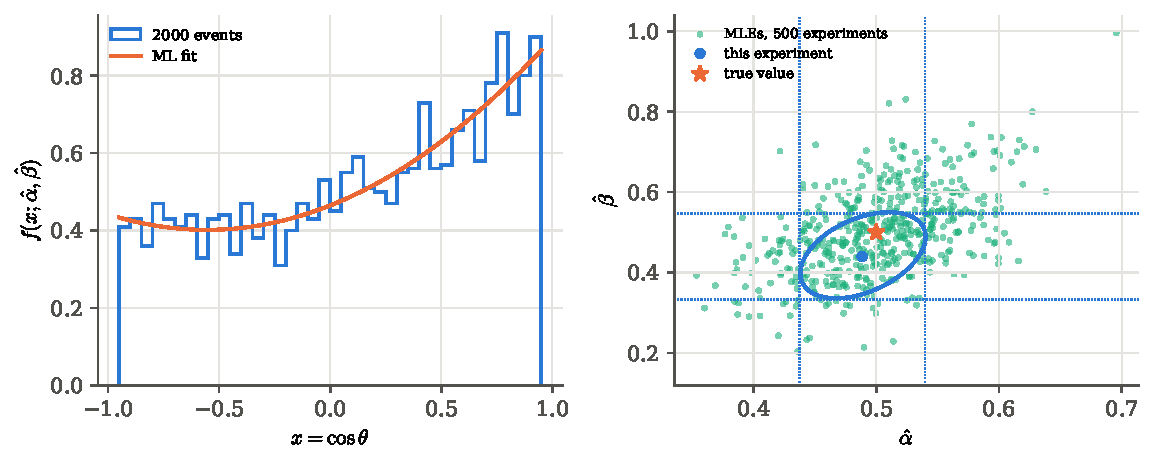
\includegraphics[width=12cm]{figures/ch03/angular_ml.pdf}
\caption{A two-parameter maximum likelihood fit. Left: $2000$ simulated
values of $\cos\theta$ and the fitted density $1+\hat\alpha x+\hat\beta x^2$
(normalised). Right: the fitted $(\hat\alpha,\hat\beta)$ of $500$ independent
repetitions of the experiment (green), the fit of the first experiment (blue
dot), the truth (star), and the contour on which $\ln\Like$ of the first
experiment has dropped by $\tfrac12$ from its maximum. The dotted lines
tangent to the contour mark $\hat\alpha\pm\sigma_{\hat\alpha}$ and
$\hat\beta\pm\sigma_{\hat\beta}$ from the inverse Hessian. The cloud of
repetitions has the size, tilt and shape of the contour.}
\label{3b:fig:angular}
\end{figure}

Repeating the whole experiment $500$ times, the maximum likelihood estimates
average $(\ThreeBAngMeanA,\ThreeBAngMeanB)$ (truth $(0.5,0.5)$) and scatter
by $\sigma_{\hat\alpha}=\ThreeBAngSdA$ and $\sigma_{\hat\beta}=\ThreeBAngSdB$.
The moment estimates scatter by $\ThreeBAngMomSdA$ and $\ThreeBAngMomSdB$.
Both methods were applied to the same $500$ data sets, so the ratios of the
spreads are measured well: $\ThreeBAngMomRatioA\pm\ThreeBAngMomRatioAErr$
for $\alpha$ and $\ThreeBAngMomRatioB\pm\ThreeBAngMomRatioBErr$ for $\beta$.
For this mild distribution the two methods are close;
the gap widens for sharply peaked densities, where low moments are poor
summaries of the shape.

\paragraph{When the number of events is itself random.}
In a counting experiment the total number of events $n$ is not fixed in
advance: it is Poisson distributed with a mean $\nu$ that the theory may
predict (a cross-section times a luminosity). Then the likelihood acquires
one more factor \srcref{Cowan}{\S6.9},
\begin{equation}
  \Like(\nu,\theta)=\frac{\nu^n e^{-\nu}}{n!}\prod_{i=1}^nf(x_i;\theta)
  =\frac{e^{-\nu}}{n!}\prod_{i=1}^n\nu f(x_i;\theta),
  \label{3b:eq:extended}
\end{equation}
the \newterm{extended likelihood}. If $\nu$ is a free parameter unrelated to
$\theta$, the $\nu$-dependent part of $\ell$ is $n\ln\nu-\nu$, whose
derivative $n/\nu-1$ vanishes at $\hat\nu=n$. The $\theta$-dependent part is
the same as before, so $\hat\theta$ is unchanged. If $\nu=\nu(\theta)$, the
total rate carries information about
$\theta$ in addition to the shape, and the extended likelihood uses both.
The product $\nu f(x;\theta)$ is the expected number of events per unit
$x$, which is why the extended likelihood is the natural starting point for
histograms of counts (\cref{3b:sec:poisson}).

\paragraph{Hidden variables.}
Some likelihoods are easy to maximise only if we knew something we were
not told, for example which of two Gaussian populations each point came
from (a mixture model). The \newterm{EM algorithm} alternates between
guessing the hidden labels from the current parameters (the ``E'' step, an
expectation) and maximising the likelihood as if the labels were known (the
``M'' step). No cycle can decrease $\Like$ \mainref{pp.~143--145}. It is
the standard tool for fitting mixtures.
\section{Gaussian noise: least squares and the \texorpdfstring{$\chi^2$}{chi-square}}
\label{3b:sec:least-squares}

Every physics student has fitted a straight line through points with error
bars by ``minimising $\chi^2$''. The rule is usually taught without a
reason. Why squares and not absolute values? Why divide by $\sigma_i^2$?
What is the error on the slope, and how do we know whether the line is any
good? All of this follows in a few lines from the likelihood of
\cref{3b:sec:likelihood}, once we assume that the noise is Gaussian. The
same lines then cover noise that is correlated from point to point, which
is the normal situation for binned power spectra and for gravitational-wave
strain. Four questions need answers.
\begin{enumerate}[label=\arabic*.]
  \item Why is least squares the maximum likelihood estimator for Gaussian
        noise, and when is it not?
  \item For a model linear in its parameters, what are the estimates and
        their covariance, exactly?
  \item What value of $\chi^2_{\min}$ should a correct model give, and how
        do we turn it into a test of the fit?
  \item What changes when the noise is correlated, and what goes wrong if
        we ignore the correlation?
\end{enumerate}

\subsection{Least squares is Gaussian maximum likelihood}
\label{3b:sec:ls-from-ml}

Take data $D_i=d_i(\params)+\epsilon_i$, $i=1,\dots,N$: the model prediction
$d_i(\params)$ plus independent noise $\epsilon_i\sim\Normal(0,\sigma_i^2)$
with known $\sigma_i$. Its log-likelihood is \eqref{3b:eq:loglike-gauss} of
\cref{3b:sec:product}. Written with the
\newterm{normalised residuals} $R_i=(D_i-d_i(\params))/\sigma_i$ it reads
\srcref{Sivia}{p.~65, (3.65)--(3.67)}
\begin{align}
  \ell(\params)
  &\eqby{1}-\frac12\sum_{i=1}^NR_i^2-\sum_{i=1}^N\ln\sqrt{2\pi}\,\sigma_i
  \eqby{2}-\frac12\chi^2(\params)+\text{const},
  \qquad
  \chi^2(\params)\equiv\sum_{i=1}^N\frac{\bigl(D_i-d_i(\params)\bigr)^2}{\sigma_i^2}.
  \label{3b:eq:chi2-def}
\end{align}
\begin{explain}
  \item \eqref{3b:eq:loglike-gauss}, with the residuals in units of their
        error bars.
  \item The error bars are known numbers, so the second sum does not
        depend on $\params$.
\end{explain}
Maximising $\ell$ is minimising $\chi^2$, because of the minus sign. So the
\newterm{least-squares estimator} is the maximum likelihood estimator
\srcref{Cowan}{\S7.1}, \srcref{HobsonBMC}{p.~50, (2.24)--(2.25)}. This
answers the two ``why'' questions. The squares come from the exponent of the
Gaussian. The $1/\sigma_i^2$ measures each residual against its own error
bar: a residual of $0.3$ is a one-sigma event for a point with
$\sigma_i=0.3$ and a ten-sigma event for a point with $\sigma_i=0.03$. With
equal error bars all points count equally. For a constant model,
$\chi^2=\sum_i(D_i-\mu)^2/\sigma_i^2$, and minimising it over $\mu$ gives
the inverse-variance weighted mean of \cref{3a:sec:weighted}.

The derivation also says when least squares is \emph{not} maximum
likelihood. It used two assumptions, and each can fail. If the noise is not
Gaussian (heavy tails, outliers, counts), the exponent is not a square. If
the error bars depend on the parameters, for example $\sigma_i^2=d_i(\params)$
for counts, the term $\sum\ln\sigma_i$ depends on $\params$ and cannot be
dropped. So least squares is what the likelihood reduces to under these two
assumptions. When it misbehaves, the cure is to go back to the likelihood,
not to patch the recipe \srcref{Sivia}{p.~66}.

\subsection{Linear models: the normal equations}
\label{3b:sec:linear-ls}

Many models are linear in their parameters even when they are not linear
in $x$: a straight line $a+bx$, a polynomial, a sum of templates with
unknown amplitudes. Write such a model as
$d_i(\params)=\sum_{k=1}^mA_{ik}\theta_k$, or $\bm d=A\params$, where the
$N\times m$ \newterm{design matrix} $A$ \unpack{column $k$ is the model
curve for $\theta_k=1$ and all other parameters zero} is known. For a line,
row $i$ of $A$ is $(1,\ x_i)$. Collect the error bars into the diagonal
covariance $\Cmat=\diag(\sigma_1^2,\dots,\sigma_N^2)$; everything below also
holds for a general $\Cmat$, which we use in \cref{3b:sec:correlated}. Then
\begin{align}
  \chi^2(\params)&\eqby{1}(\bm D-A\params)\T\Cmat^{-1}(\bm D-A\params),
  \nonumber\\
  \frac{\partial\chi^2}{\partial\params}&\eqby{2}-2A\T\Cmat^{-1}(\bm D-A\params)
  \eqby{3}\bm0
  \quad\Longrightarrow\quad
  (A\T\Cmat^{-1}A)\,\hat\params=A\T\Cmat^{-1}\bm D,
  \nonumber\\
  \hat\params&\eqby{4}(A\T\Cmat^{-1}A)^{-1}A\T\Cmat^{-1}\bm D
  \;\equiv\;B\bm D .
  \label{3b:eq:normal-eq}
\end{align}
\begin{explain}
  \item With a diagonal $\Cmat$ this is
        $\sum_i(D_i-d_i)^2/\sigma_i^2$ written as a matrix product.
  \item Differentiate the quadratic form: for a symmetric matrix $M$,
        $\partial(\bm v\T M\bm v)/\partial\params=2(\partial\bm v/\partial\params)\T M\bm v$,
        and here $\partial\bm v/\partial\params=-A$.
  \item The score equation. These $m$ linear equations are the
        \newterm{normal equations}.
  \item The matrix $A\T\Cmat^{-1}A$ is $m\times m$ and invertible as long as
        the columns of $A$ are linearly independent (no two parameters do the
        same thing to the model).
\end{explain}
The estimator is a fixed matrix $B$ times the data. So its mean and
covariance follow from linear error propagation, which is exact for linear
maps (\cref{3a:sec:linear-exact}):
\begin{align}
  \E\hat\params&\eqby{1}B\,\E\bm D\eqby{2}(A\T\Cmat^{-1}A)^{-1}A\T\Cmat^{-1}A\params=\params,
  \nonumber\\
  \Cov\hat\params&\eqby{3}B\,\Cmat\,B\T
  \eqby{4}(A\T\Cmat^{-1}A)^{-1}A\T\Cmat^{-1}\,\Cmat\,\Cmat^{-1}A(A\T\Cmat^{-1}A)^{-1}
  \eqby{5}(A\T\Cmat^{-1}A)^{-1}\equiv U .
  \label{3b:eq:ls-cov}
\end{align}
\begin{explain}
  \item Expectation is linear.
  \item The noise has mean zero, so $\E\bm D=A\params$.
  \item Covariance of a linear map, $\Cov(B\bm D)=B\Cov(\bm D)B\T$.
  \item Insert $B$ and $B\T$; $\Cmat$ and $A\T\Cmat^{-1}A$ are symmetric.
  \item $\Cmat^{-1}\Cmat=\Id$, and then
        $(A\T\Cmat^{-1}A)^{-1}(A\T\Cmat^{-1}A)=\Id$.
\end{explain}
So for a linear model with Gaussian noise the least-squares estimates are
unbiased and have covariance $U=(A\T\Cmat^{-1}A)^{-1}$, with no
approximation. Now look at the curvature of $\chi^2$. Differentiating
\eqref{3b:eq:normal-eq} once more gives
$\partial^2\chi^2/\partial\params\,\partial\params\T=2A\T\Cmat^{-1}A=2U^{-1}$.
Because $\chi^2$ is exactly quadratic in $\params$, its Taylor series stops
there:
\begin{equation}
  \chi^2(\params)=\chi^2_{\min}+(\params-\hat\params)\T U^{-1}(\params-\hat\params),
  \qquad
  \ell(\params)=\ell_{\max}-\tfrac12(\params-\hat\params)\T U^{-1}(\params-\hat\params).
  \label{3b:eq:chi2-quadratic}
\end{equation}
The likelihood is an exact Gaussian in $\params$, centred on $\hat\params$,
whose width matrix is the covariance of the estimator. In one dimension
$\chi^2(\theta)=\chi^2_{\min}+(\theta-\hat\theta)^2/\sigma_{\hat\theta}^2$,
so the parameter values at which $\chi^2$ has risen by one from its minimum
are exactly $\hat\theta\pm\sigma_{\hat\theta}$ \srcref{Cowan}{\S7.2}.
This is the model case for the rule ``the curvature of the log-likelihood is
the error'', which \cref{3b:sec:curvature} extends to every smooth
likelihood.

\begin{keyidea}[Linear least squares]
For data $\bm D=A\params+\bm\epsilon$ with Gaussian noise of covariance
$\Cmat$,
\[
  \hat\params=(A\T\Cmat^{-1}A)^{-1}A\T\Cmat^{-1}\bm D,\qquad
  \Cov\hat\params=(A\T\Cmat^{-1}A)^{-1},
\]
the estimator is unbiased and Gaussian, and $\chi^2$ rises by exactly one at
$\hat\theta_k\pm\sigma_{\hat\theta_k}$ when the other parameters are
re-minimised. Nothing here is asymptotic.
\end{keyidea}

\paragraph{Example: a straight line through three points.}
Fit $y=a+bx$ to $(x_i,y_i)=(0,1.1),(1,1.9),(2,3.2)$, all with $\sigma=0.1$.
For a line the normal equations are $2\times2$, and it pays to name the sums
$S=\sum1/\sigma_i^2$, $S_x=\sum x_i/\sigma_i^2$, $S_{xx}=\sum x_i^2/\sigma_i^2$,
$S_y=\sum y_i/\sigma_i^2$, $S_{xy}=\sum x_iy_i/\sigma_i^2$ and
$\Delta=SS_{xx}-S_x^2$. In units of $1/\sigma^2=100$ they are $S=3$,
$S_x=3$, $S_{xx}=5$, $S_y=6.2$, $S_{xy}=8.3$. Then
\begin{align*}
  \begin{pmatrix}\hat a\\ \hat b\end{pmatrix}
  &\eqby{1}\begin{pmatrix}S&S_x\\ S_x&S_{xx}\end{pmatrix}^{-1}
    \begin{pmatrix}S_y\\ S_{xy}\end{pmatrix}
  \eqby{2}\frac1\Delta\begin{pmatrix}S_{xx}S_y-S_xS_{xy}\\ SS_{xy}-S_xS_y\end{pmatrix}
  =\frac16\begin{pmatrix}31-24.9\\ 24.9-18.6\end{pmatrix}
  =\begin{pmatrix}1.017\\ 1.050\end{pmatrix},\\
  U&\eqby{3}\frac1\Delta\begin{pmatrix}S_{xx}&-S_x\\ -S_x&S\end{pmatrix}
  =\sigma^2\begin{pmatrix}5/6&-1/2\\ -1/2&1/2\end{pmatrix},
  \qquad
  \sigma_{\hat a}=0.091,\ \ \sigma_{\hat b}=0.071,\ \ \rho=-0.775 .
\end{align*}
\begin{explain}
  \item The normal equations \eqref{3b:eq:normal-eq}: with rows $(1,x_i)$,
        $A\T\Cmat^{-1}A$ has entries $S,S_x,S_x,S_{xx}$ and
        $A\T\Cmat^{-1}\bm y=(S_y,S_{xy})\T$.
  \item Inverse of a $2\times2$ matrix: swap the diagonal, negate the
        off-diagonal, divide by the determinant $\Delta$. Here
        $\Delta=3\cdot5-3^2=6$ in units of $\sigma^{-4}$; the powers of
        $\sigma$ cancel in $\hat a,\hat b$.
  \item $U=(A\T\Cmat^{-1}A)^{-1}$ from \eqref{3b:eq:ls-cov}; restoring the
        units, $1/\Delta=\sigma^4/6$ and the matrix entries carry
        $1/\sigma^2$.
\end{explain}
The intercept and slope are strongly anticorrelated, $\rho=-(1/2)/\sqrt{(5/6)(1/2)}$:
if the fitted slope is a little too steep, the line must start a little
lower to pass through the middle of the data. Choosing the origin of $x$
at the weighted mean, $\bar x=S_x/S=1$, would make $S_x=0$ and the two
estimates uncorrelated. The residuals are $y_i-\hat a-\hat bx_i=(0.083,-0.167,0.083)$,
so $\chi^2_{\min}=(0.0069+0.0278+0.0069)/0.01=4.17$. Is that good or bad?

\subsection{How good is the fit? The distribution of \texorpdfstring{$\chi^2_{\min}$}{chi2min}}
\label{3b:sec:chi2-min}

If the model is right, every normalised residual is a standard Gaussian
before fitting, and $\chi^2(\params_{\text{true}})$ is a sum of $N$ squared
standard Gaussians, so it follows the $\chi^2_N$ distribution (\cref{ch:02}).
Fitting lowers it: the fitted curve bends towards the data and eats part
of the noise. By how much? The cleanest way to see it is geometric.

Whiten the data first. Factor the covariance as $\Cmat=LL\T$ (for a
diagonal $\Cmat$, simply $L=\diag(\sigma_i)$; in general the Cholesky
factor). Then $\bm z=L^{-1}\bm D$, $\tilde A=L^{-1}A$ and
$\bm\eta=L^{-1}\bm\epsilon$ satisfy $\bm z=\tilde A\params+\bm\eta$ with
$\bm\eta\sim\Normal(\bm0,\Id_N)$, and
$\chi^2=|\bm z-\tilde A\params|^2$ is an ordinary squared distance in
$\R^N$. The model predictions $\tilde A\params$, as $\params$ ranges over
$\R^m$, fill an $m$-dimensional flat subspace (the column space of
$\tilde A$). Minimising the distance means dropping a perpendicular:
the fit is the orthogonal projection of $\bm z$ onto that subspace
(\cref{3b:fig:projection}). With the projector
$P=\tilde A(\tilde A\T\tilde A)^{-1}\tilde A\T$
\unpack{the matrix that maps any vector to its closest point in the model
subspace. It satisfies $P^2=P$ and $P\T=P$},
\begin{align}
  \chi^2_{\min}
  &\eqby{1}\bigl|(\Id-P)\bm z\bigr|^2
  \eqby{2}\bigl|(\Id-P)\bm\eta\bigr|^2
  \eqby{3}\bm\eta\T(\Id-P)\bm\eta ,
  \nonumber\\
  \E\chi^2_{\min}
  &\eqby{4}\tr\bigl[(\Id-P)\,\E(\bm\eta\bm\eta\T)\bigr]
  \eqby{5}\tr(\Id_N)-\tr P
  \eqby{6}N-m\equiv\dof .
  \label{3b:eq:chi2-min-mean}
\end{align}
\begin{explain}
  \item The fitted point is $P\bm z$, so the residual vector is
        $\bm z-P\bm z$.
  \item $\bm z=\tilde A\params+\bm\eta$, and $(\Id-P)\tilde A=0$ because
        $P$ leaves every vector of the model subspace unchanged. The true
        model drops out: only the noise is left.
  \item $|\bm v|^2=\bm v\T\bm v$ with $(\Id-P)\T(\Id-P)=\Id-P$, using
        $P\T=P$ and $P^2=P$.
  \item A number equals its own trace, $\bm\eta\T M\bm\eta=\tr(M\bm\eta\bm\eta\T)$,
        and the trace is linear, so it commutes with $\E$.
  \item Whitened noise has $\E(\bm\eta\bm\eta\T)=\Id_N$.
  \item $\tr P=\tr[(\tilde A\T\tilde A)^{-1}\tilde A\T\tilde A]=\tr\Id_m=m$,
        by the cyclic property of the trace.
\end{explain}
The fit removes on average exactly one unit of $\chi^2$ per fitted
parameter. The whole distribution follows too. $P$ is a projector of rank
$m$, so it has $m$ eigenvalues $1$ and $N-m$ eigenvalues $0$, and $\Id-P$
has the reverse. Rotate to the eigenbasis of $P$. A rotation of independent
standard Gaussians gives independent standard Gaussians again, because
$\Normal(\bm0,\Id)$ looks the same in every direction. In the new basis
$\chi^2_{\min}=\bm\eta\T(\Id-P)\bm\eta$ keeps only the $N-m$ components
with eigenvalue $1$, so it is a sum of $N-m$ squared independent standard
Gaussians:
\begin{equation}
  \chi^2_{\min}\sim\chi^2_{\dof},\qquad \dof=N-m,\qquad
  \E\chi^2_{\min}=\dof,\qquad \Var\chi^2_{\min}=2\dof .
  \label{3b:eq:chi2-min-dist}
\end{equation}
This is the argument that gave the divisor $N-1$ in the sample variance
(\cref{3a:sec:n-minus-one}), where one parameter, the mean, was fitted. Now
there are $m$. The number $\dof$ is the number of \newterm{degrees of
freedom} of the fit.

\begin{figure}[htbp]
\centering
\begin{tikzpicture}[x={(1.3cm,0cm)},y={(0.62cm,0.42cm)},z={(0cm,1.2cm)}]
  \fill[formblue!10] (-0.3,-0.4,0) -- (3.6,-0.4,0) -- (3.6,2.6,0) -- (-0.3,2.6,0) -- cycle;
  \draw[formblue!60] (-0.3,-0.4,0) -- (3.6,-0.4,0) -- (3.6,2.6,0) -- (-0.3,2.6,0) -- cycle;
  \node[font=\footnotesize,formblue,anchor=west] at (3.65,2.4,0) {model subspace $\{\tilde A\params\}$};
  \coordinate (O) at (0,0,0);
  \coordinate (T) at (1.7,1.2,0);
  \coordinate (Z) at (2.3,1.7,1.5);
  \coordinate (F) at (2.3,1.7,0);
  \draw[vec,black!70] (O) -- (Z);
  \draw[vec,formblue] (O) -- (F);
  \draw[fibre,->] (T) -- (Z);
  \draw[bdry,->] (F) -- (Z);
  \draw[faint,densely dashed] (T) -- (F);
  \draw[faint] ($(F)+(0,0,0.18)$) -- ($(F)+(0,0,0.18)+(0.12,0.1,0)$) -- ($(F)+(0.12,0.1,0)$);
  \fill (O) circle (1.3pt); \fill (T) circle (1.3pt); \fill (Z) circle (1.5pt); \fill (F) circle (1.3pt);
  \node[font=\footnotesize,anchor=east] at (O) {$0$};
  \node[font=\footnotesize,anchor=north] at (T) {$\tilde A\params_{\text{true}}$};
  \node[font=\footnotesize,anchor=south] at (Z) {data $\bm z$};
  \node[font=\footnotesize,anchor=north west] at (F) {fit $P\bm z=\tilde A\hat\params$};
  \node[font=\footnotesize,align=left,anchor=north west] at (-0.3,-0.9,0)
       {\textcolor{fibreorange}{orange}: noise $\bm\eta$ ($N$ dimensions)\quad
        \textcolor{bdryred}{red}: residual $(\Id-P)\bm\eta$ ($N-m$ dimensions)};
\end{tikzpicture}
\caption{Least squares as a projection, after whitening so that the noise is
the same in every direction. The data vector lies off the model subspace by
the noise vector (orange). The fit drops a perpendicular onto the subspace.
The residual (red) is the part of the noise perpendicular to the subspace;
the part lying inside it has been absorbed into the fitted parameters,
which is why the fit sits away from the truth along the plane. With $m$
parameters, $m$ of the $N$ noise components are absorbed and $N-m$ are left
in $\chi^2_{\min}$.}
\label{3b:fig:projection}
\end{figure}

\paragraph{Turning $\chi^2_{\min}$ into a test.}
Given \eqref{3b:eq:chi2-min-dist}, a correct model with correct error bars
gives $\chi^2_{\min}\approx\dof\pm\sqrt{2\dof}$. The standard summary is
the \newterm{goodness-of-fit $p$-value}, the probability that a correct
model would give a $\chi^2_{\min}$ at least as large as the one observed,
$\pval=\Prob(\chi^2_\dof\ge\chi^2_{\min})$ \srcref{Padilla}{\S3.5},
\srcref{Cowan}{\S7.5}. A tiny $\pval$ says that the data are hard to
reconcile with the model and the error bars together: the model is wrong,
or the errors are underestimated, or the noise is not Gaussian. A
$\pval$ very close to one ($\chi^2_{\min}\ll\dof$) is also a warning: the
errors are overestimated, or there are correlations that were ignored
(\cref{3b:sec:correlated}), or the data were ``cleaned'' by hand. The
ratio $\chi^2_{\min}/\dof$, the \newterm{reduced} $\chi^2$, should be near
one, with a spread of $\sqrt{2/\dof}$. The full logic of tests, and what a
$p$-value does and does not mean, is \cref{ch:04}.

\paragraph{Example: the three-point line again.}
Two parameters from three points leave $\dof=1$. The observed
$\chi^2_{\min}=4.17$ has
$\pval=\Prob(\chi^2_1\ge4.17)=\Prob(|Z|\ge2.04)=0.041$, where
$Z\sim\Normal(0,1)$ and we used that a $\chi^2_1$ variable is the square of
one standard Gaussian. Such a large $\chi^2$ happens in about four per cent
of experiments if the line and the error bars are both right. With one
degree of freedom this is weak evidence, but it would be worth checking
whether $\sigma=0.1$ is honest.

\paragraph{Confidence regions from $\Delta\chi^2$.}
The quadratic form \eqref{3b:eq:chi2-quadratic}, evaluated at the true
parameters, is
$\chi^2(\params_{\text{true}})-\chi^2_{\min}=(\hat\params-\params_{\text{true}})\T U^{-1}(\hat\params-\params_{\text{true}})$,
and since $\hat\params-\params_{\text{true}}\sim\Normal(\bm0,U)$, it is a
sum of $m$ squared standard Gaussians (whiten with $U$ as we whitened with
$\Cmat$): $\Delta\chi^2\sim\chi^2_m$. The region
$\{\params:\chi^2(\params)\le\chi^2_{\min}+\Delta\chi^2_\alpha\}$ therefore
covers the truth in a fraction $1-\alpha$ of repeated experiments if
$\Delta\chi^2_\alpha$ is the corresponding quantile of $\chi^2_m$
\srcref{Padilla}{\S3.6, Table~III}:
\begin{center}
\small
\begin{tabular}{lccc}
  \hline
  coverage & $m=1$ & $m=2$ & $m=3$\\
  \hline
  $68.3\%$ & $1.00$ & $2.30$ & $3.53$\\
  $95.4\%$ & $4.00$ & $6.17$ & $8.02$\\
  $99.73\%$ & $9.00$ & $11.8$ & $14.2$\\
  \hline
\end{tabular}
\end{center}
The threshold depends on the number $m$ of parameters in the joint region,
not on the number $N$ of data points.\footnote{Padilla et al.\ write the recipe
as $Q(n-M,\min\chi^2+\Delta\chi^2)=p$ \srcref{Padilla}{(37)}, which mixes
the goodness-of-fit distribution (with $n-M$ degrees of freedom) with the
distribution of $\Delta\chi^2$ (with $M$). Their Table~III is correct and
follows from $\Prob(\chi^2_M\le\Delta\chi^2)=p$.} For one parameter at a
time, with the others re-minimised, $\Delta\chi^2=1$ gives the
$\hat\theta\pm\sigma_{\hat\theta}$ interval found from
\eqref{3b:eq:chi2-quadratic}. A joint two-parameter $68\%$ region needs
$\Delta\chi^2=2.30$, a larger ellipse. Since $\ell=-\tfrac12\chi^2+\text{const}$,
the same ellipse is the contour on which $\ln\Like$ has dropped by
$2.30/2$ from its maximum (\cref{3b:sec:curvature}).

\subsection{Fitting a line in Python}
\label{3b:sec:ls-python}

The script \pyname{11_line_fit.py} fits $y=a+bx$ to $N=10$ points at
$x=1,\dots,10$ with error bars growing from $0.48$ to $1.2$, true values
$a=1$, $b=0.5$. The whole of linear least squares is five lines.
\pyfile[firstline=30,lastline=37]{code/ch03/11_line_fit.py}{Generalised least squares in five lines}
Line by line: invert the covariance, form $U=(A\T\Cmat^{-1}A)^{-1}$, apply
\eqref{3b:eq:normal-eq}, form the residuals and
$\chi^2=\bm r\T\Cmat^{-1}\bm r$. The function accepts a whole stack of data
sets at once (one per row of \pyname{y}), which is how we fit $10^4$
simulated experiments in one call.

For the first data set the fit gives $\hat a=\ThreeBLineA\pm\ThreeBLineSa$,
$\hat b=\ThreeBLineB\pm\ThreeBLineSb$ with correlation $\ThreeBLineRho$,
and $\chi^2_{\min}=\ThreeBLineChi$ for $\dof=8$, a goodness-of-fit
$\pval=\ThreeBLineP$: an unremarkable fit. Over $10^4$ repetitions the
estimates scatter by $\ThreeBLineSaMC$ and $\ThreeBLineSbMC$ with
correlation $\ThreeBLineRhoMC$, exactly as $U$ predicts, and
$\chi^2_{\min}$ has mean $\ThreeBLineChiMean$ and variance
$\ThreeBLineChiVar$, against $\dof=8$ and $2\dof=16$ from
\eqref{3b:eq:chi2-min-dist}. Fitting the wrong model, a constant, to the same
data gives an average $\chi^2_{\min}$ of $\ThreeBLineWrongMean$ for $9$
degrees of freedom: the test sees the missing slope at once
(\cref{3b:fig:line-fit}).

\begin{figure}[htbp]
\centering
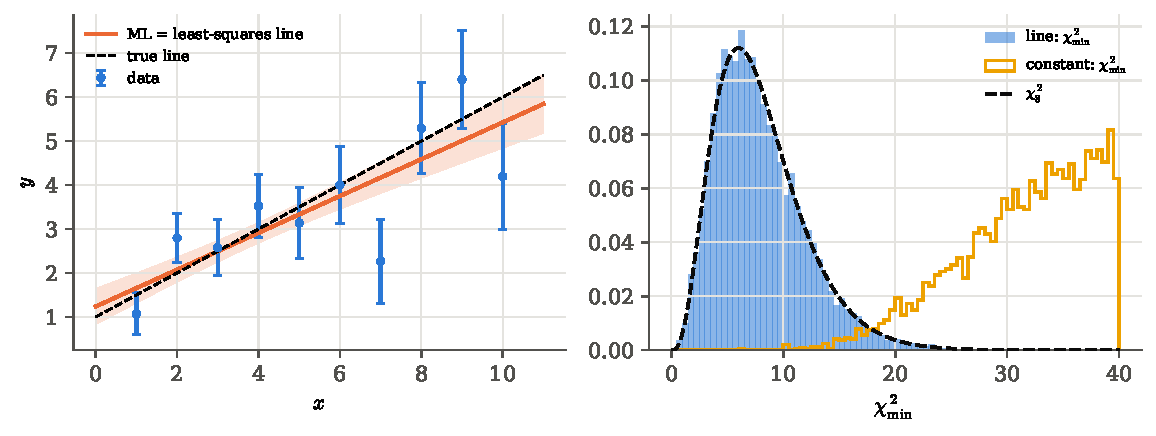
\includegraphics[width=12cm]{figures/ch03/line_fit.pdf}
\caption{Least squares as Gaussian maximum likelihood. Left: ten points with
error bars that grow to the right, the fitted line with its $\pm1\sigma$
band from $U=(A\T\Cmat^{-1}A)^{-1}$ (narrowest near the weighted centre of
the data), and the true line (dashed). Right: $\chi^2_{\min}$ of $10^4$
simulated experiments for the correct model (filled), which follows the
$\chi^2_8$ curve, and for a constant fitted to the same data (outline), which
sits far to the right.}
\label{3b:fig:line-fit}
\end{figure}

\subsection{Correlated noise: \texorpdfstring{$\chi^2=\bm r\T\Cmat^{-1}\bm r$}{chi2 = r C-1 r}}
\label{3b:sec:correlated}

Noise is often correlated from one data point to the next. Neighbouring
bins of a power spectrum share modes. A slowly drifting baseline pushes
consecutive readings up together. A common calibration error moves every
point at once.
The noise is then a Gaussian vector $\bm\epsilon\sim\Normal(\bm0,\Cmat)$ with
a non-diagonal covariance, and the likelihood is the multivariate normal
density (\cref{ch:02}) evaluated at the required noise
$\bm r=\bm D-\bm d(\params)$:
\begin{align}
  \Like(\params)
  &\eqby{1}p_{\bm\eta}\bigl(L^{-1}\bm r\bigr)\,\bigl|\det L^{-1}\bigr|
  \eqby{2}\frac{1}{(2\pi)^{N/2}}\,e^{-\frac12(L^{-1}\bm r)\T(L^{-1}\bm r)}\,
   \frac{1}{|\det L|}
  \nonumber\\
  &\eqby{3}\frac{1}{\sqrt{(2\pi)^N\det\Cmat}}
   \exp\!\Bigl[-\tfrac12\,\bm r\T\Cmat^{-1}\bm r\Bigr],
  \qquad
  -2\ell(\params)=\bm r\T\Cmat^{-1}\bm r+\ln\det\Cmat+N\ln2\pi .
  \label{3b:eq:like-corr}
\end{align}
\begin{explain}
  \item Write the noise as $\bm\epsilon=L\bm\eta$ with $\Cmat=LL\T$ and
        $\bm\eta\sim\Normal(\bm0,\Id)$. Changing variables from $\bm\eta$ to
        $\bm\epsilon$ multiplies the density by the Jacobian
        $|\det(\partial\bm\eta/\partial\bm\epsilon)|=|\det L^{-1}|$.
  \item Independent standard Gaussians: the density is the product of $N$
        factors $(2\pi)^{-1/2}e^{-\eta_i^2/2}$.
  \item $(L^{-1}\bm r)\T(L^{-1}\bm r)=\bm r\T(LL\T)^{-1}\bm r=\bm r\T\Cmat^{-1}\bm r$,
        and $(\det L)^2=\det\Cmat$.
\end{explain}
So the correlated $\chi^2$ is $\bm r\T\Cmat^{-1}\bm r$, and every result
above, from the normal equations to $\chi^2_{\min}\sim\chi^2_{N-m}$,
holds with this $\Cmat$, because those derivations never used that $\Cmat$
was diagonal. This is the likelihood written for cosmological data with
correlated errors. One term needs care. The $\ln\det\Cmat$ is a constant
only if the covariance does not depend on the parameters. For the power
spectrum of a Gaussian random field the
covariance \emph{is} the signal (cosmic variance scales with $\Cell$
itself), and then $\ln\det\Cmat(\params)$ must be kept. Dropping it biases
the fit (\cref{ch:07}).

\paragraph{What goes wrong if we ignore the correlation?}
Suppose the noise has covariance $\Cmat_{ij}=\sigma_i\sigma_je^{-|x_i-x_j|/2}$
(neighbours correlated at $e^{-1/2}=0.61$) but we fit with only the
diagonal. The estimator is still $\hat\params=B_{\text{diag}}\bm D$, a
linear function of the data with $B_{\text{diag}}A=\Id$, so it is still
\emph{unbiased}. What is wrong is the error bar. The quoted covariance
$(A\T\Cmat_{\text{diag}}^{-1}A)^{-1}$ assumes the noise we did not have; the
true covariance is $B_{\text{diag}}\Cmat B_{\text{diag}}\T$ by the same
propagation rule as \eqref{3b:eq:ls-cov}. The second half of
\pyname{11_line_fit.py} draws correlated noise as $L\bm\eta$ with the
Cholesky factor and fits $10^4$ data sets both ways. For the slope:
\begin{center}
\small
\begin{tabular}{lccc}
  \hline
  fit & mean $\hat b$ & quoted $\sigma_{\hat b}$ & true scatter of $\hat b$\\
  \hline
  diagonal $\chi^2$ & $\ThreeBCorrMeanBd$ & $\ThreeBCorrQuoted$ & $\ThreeBCorrSdD$ (predicted $\ThreeBCorrTrueD$)\\
  full $\bm r\T\Cmat^{-1}\bm r$ & $\ThreeBCorrMeanBf$ & $\ThreeBCorrQuotedF$ & $\ThreeBCorrSdF$\\
  \hline
\end{tabular}
\end{center}
Both fits centre on the true slope $0.5$. The diagonal fit claims an error
of $\ThreeBCorrQuoted$ but actually scatters by $\ThreeBCorrSdD$, so every
quoted interval is too short by a third. The full fit quotes its error
correctly, and that error is also smaller than the true error of the
diagonal fit: using the correlations is not only honest but more precise.
The goodness of fit misleads too. With the diagonal $\chi^2$ the average
$\chi^2_{\min}$ is $\ThreeBCorrChiD$ instead of $8$, a fit that looks
suspiciously good; with the full $\Cmat$ it is $\ThreeBCorrChiF$
(\cref{3b:fig:line-fit-corr}).

\begin{pitfall}[Correlated noise makes a bad error bar look like a good fit]
Positively correlated noise moves neighbouring points up and down
together. A smooth model can follow such coherent wiggles, so the residuals
come out smaller than independent noise of the same size would give, and
$\chi^2_{\min}\ll\dof$. At the same moment the parameter errors computed from
the diagonal are too small. A reduced $\chi^2$ well below one is a hint to
look for correlations, not a reason to celebrate.
\end{pitfall}

\begin{figure}[htbp]
\centering
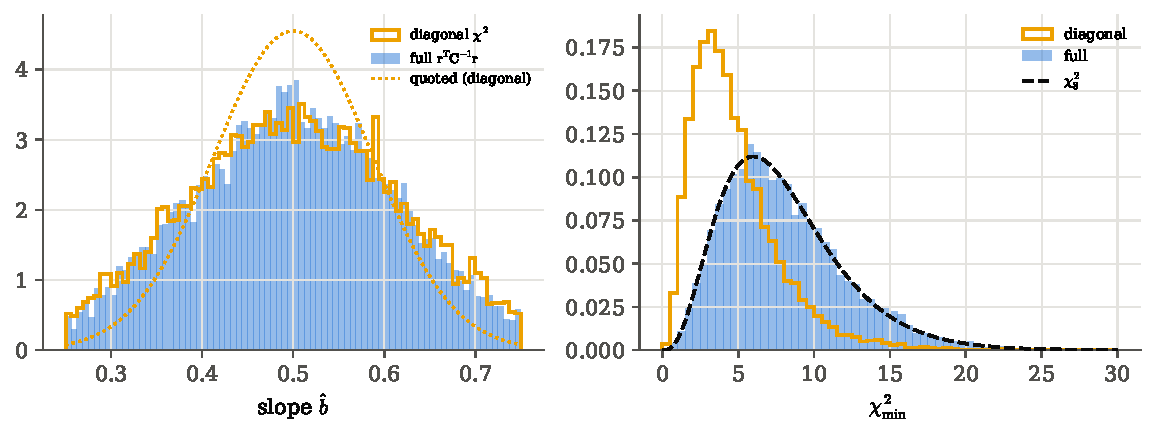
\includegraphics[width=12cm]{figures/ch03/line_fit_corr.pdf}
\caption{Fitting data with correlated noise, $10^4$ simulated experiments.
Left: the slope from the diagonal $\chi^2$ (outline) and from the full
$\bm r\T\Cmat^{-1}\bm r$ (filled). Both are centred on the truth, but the
diagonal fit is wider than the Gaussian it quotes (dotted). Right: the
diagonal fit's $\chi^2_{\min}$ piles up well below the $\chi^2_8$ curve,
while the full fit's follows it.}
\label{3b:fig:line-fit-corr}
\end{figure}

\paragraph{The same idea for a gravitational-wave detector.}
Detector noise is correlated in time but, if stationary, it is uncorrelated
between different frequencies: the Fourier transform diagonalises its
covariance, and the diagonal entries are the noise power spectral density
$S_n(f)$ \unpack{the noise variance per unit frequency. Frequencies where the
detector is noisy have large $S_n$}. The sum $\bm r\T\Cmat^{-1}\bm r$ then
becomes an integral over frequency, with $\tilde r(f)=\int r(t)e^{-2\pi ift}\dd t$,
\[
  -2\ell(\params)=(D-h_{\params}\,|\,D-h_{\params})+\text{const},\qquad
  (a\,|\,b)\equiv4\,\mathrm{Re}\int_0^\infty\frac{\tilde a(f)\,\tilde b^*(f)}{S_n(f)}\,\dd f ,
\]
where $h_{\params}$ is the waveform predicted for source parameters
$\params$. The \newterm{noise-weighted inner product} $(a|b)$ is
$\bm a\T\Cmat^{-1}\bm b$ in the basis where $\Cmat$ is diagonal, with
one-sided $S_n$ and positive frequencies only, hence the factor $4$. Every
gravitational-wave parameter estimate, and the Fisher forecasts of
\cref{ch:10}, start from this one line.
\section{Counting experiments: the Poisson likelihood of a histogram}
\label{3b:sec:poisson}

A search at a collider histograms the invariant mass of candidate events
into bins; an X-ray telescope histograms photon energies; a decay experiment
histograms decay times. Far from the peak, or in a short run, many bins hold
a handful of events, and some hold none. The habit of putting an error bar
$\sqrt{n_i}$ on every bin and minimising $\chi^2$ breaks down here. A bin
with $n_i=0$ gets an error bar of zero, and bins that fluctuated low get
error bars that are too small. The reason is that the noise in a counting
experiment is not Gaussian and is not added to the prediction. The count in
a bin is a Poisson random number whose mean is the prediction. The
likelihood has no trouble with this, because all it needs is the
probability of what was observed. Four questions need answers.
\begin{enumerate}[label=\arabic*.]
  \item What is the likelihood of a histogram of counts, and what does
        maximising it do to the total number of events?
  \item Can the same likelihood also tell us whether the fit is good?
  \item What exactly goes wrong with the two $\chi^2$ recipes that use
        $\sqrt{n_i}$ or $\sqrt{\mu_i}$ as the error bar?
  \item How does the idea carry over to other data: measurements with
        Gaussian errors, gravitational-wave strain, CMB maps?
\end{enumerate}

\subsection{The likelihood of a histogram}
\label{3b:sec:poisson-like}

Divide the range of $x$ into $N$ bins. If events arrive independently at a
constant rate, the count $n_i$ in bin $i$ is Poisson distributed
(\cref{ch:02}) with mean
\[
  \mu_i(\nu,\params)=\nu\int_{\text{bin }i}f(x;\params)\,\dd x\equiv\nu\,p_i(\params),
  \qquad\sum_{i=1}^Np_i(\params)=1,
\]
where $\nu$ is the expected total and $p_i$ the probability that an event
falls in bin $i$ \srcref{Cowan}{\S6.10}. Different bins are independent,
so
\begin{align}
  \Like(\nu,\params)
  &\eqby{1}\prod_{i=1}^N\frac{\mu_i^{n_i}e^{-\mu_i}}{n_i!},
  \nonumber\\
  \ell(\nu,\params)
  &\eqby{2}\sum_{i=1}^N\bigl(n_i\ln\mu_i-\mu_i\bigr)-\sum_{i=1}^N\ln n_i!
  \eqby{3}-\tfrac12\,C(\nu,\params)+\text{const},
  \qquad
  C\equiv2\sum_{i=1}^N\bigl(\mu_i-n_i\ln\mu_i\bigr).
  \label{3b:eq:poisson-like}
\end{align}
\begin{explain}
  \item Poisson probability of $n_i$ counts for mean $\mu_i$, multiplied over
        independent bins \srcref{Cowan}{(6.44)}.
  \item $\ln(\mu^ne^{-\mu}/n!)=n\ln\mu-\mu-\ln n!$.
  \item The counts are data, so $\sum\ln n_i!$ does not depend on the
        parameters.
\end{explain}
The quantity $C=-2\ell+\text{const}$ is the \newterm{Cash statistic},
introduced for X-ray astronomy \cite{Cash1979}; minimising it is
maximising the Poisson likelihood. In the language of
\cref{3b:sec:likelihood}, each bin asks how probable it is that a Poisson
source with mean $\mu_i(\params)$ produced the count we saw, and an empty
bin contributes simply $e^{-\mu_i}$, the probability of seeing nothing.

\paragraph{The total number of events is conserved.}
Split the Poisson product into a statement about the total and a
statement about the shape. With $n=\sum_in_i$ and $\mu_i=\nu p_i$,
\begin{align}
  \prod_{i=1}^N\frac{\mu_i^{n_i}e^{-\mu_i}}{n_i!}
  &\eqby{1}\frac{\nu^{n}e^{-\nu}}{n!}\;
   \frac{n!}{\prod_in_i!}\prod_{i=1}^Np_i^{n_i},
  \label{3b:eq:poisson-split}\\
  \frac{\partial\ell}{\partial\nu}
  &\eqby{2}\frac{n}{\nu}-1\eqby{3}0
  \quad\Longrightarrow\quad\hat\nu=n .
  \nonumber
\end{align}
\begin{explain}
  \item $\prod_i\mu_i^{n_i}=\nu^{\sum n_i}\prod_ip_i^{n_i}$ and
        $\prod_ie^{-\mu_i}=e^{-\nu\sum p_i}=e^{-\nu}$; then multiply and
        divide by $n!$. The first factor is the Poisson probability of the
        total, the second the multinomial probability of the split into bins
        \srcref{Cowan}{(6.41), (6.43)}.
  \item Only the first factor depends on $\nu$, and
        $\partial_\nu(n\ln\nu-\nu)=n/\nu-1$.
  \item The score equation for $\nu$; the multinomial factor is untouched,
        so $\hat\params$ is the same as in a fit with the total fixed.
\end{explain}
The fitted normalisation equals the observed number of events, exactly, in
every experiment, whatever the shape parameters do. This is the binned form
of the extended likelihood \eqref{3b:eq:extended}. It is also the property
the two $\chi^2$ recipes below lack.

\begin{workdef}[Poisson likelihood of a histogram]
For counts $n_i$ with predicted means $\mu_i(\params)$,
\[
  -2\ell(\params)=2\sum_i\bigl(\mu_i-n_i\ln\mu_i\bigr)+\text{const}.
\]
\emph{Operationally:} compute the expected count in every bin from the
model (integrate the density over the bin and multiply by the expected
total), evaluate this sum, minimise. Empty bins stay in the sum and
contribute $2\mu_i$. No bins need to be merged, and no error bars are
assigned.
\end{workdef}

\paragraph{Example: one bin.}
For a single bin with $n=9$ counts,
$\ell(\mu)=9\ln\mu-\mu$ gives $\hat\mu=9$ and
$-\ell''(\hat\mu)=n/\hat\mu^2=1/9$, a curvature error of $3=\sqrt n$, the
familiar rule. The likelihood itself is skewed: solving
$\ell(\mu)=\ell_{\max}-\tfrac12$ gives $\mu\in[6.32,12.34]$, that is
$9^{+3.34}_{-2.68}$. The interval reaches further up than down. Why? A
Poisson count with mean $\mu$ has spread $\sqrt\mu$. A large mean such as
$12.34$ has a large spread, $3.5$, so a count of $9$ is less than one spread
below it. A small mean such as $6.32$ has a small spread, $2.5$, so the
same count is slightly more than one spread above it. Large means can
therefore stray further from the data and still explain them about as well
(\cref{3b:sec:curvature}).

\subsection{Fitting and testing with one number: the Baker--Cousins \texorpdfstring{$\chi^2_\lambda$}{chi2-lambda}}
\label{3b:sec:baker-cousins}

The value of $C$ at its minimum does not by itself say whether the fit is
good. Its constant is arbitrary, and it grows with the total number of
events even for a perfect model. To make it a measure of fit, compare the
model with the best any model could do \cite{BakerCousins1984}. That best
is the \newterm{saturated model}
\unpack{a ``model'' with one free mean per bin, which therefore sets
$\mu_i=n_i$ and fits the data perfectly}. The likelihood ratio is
\begin{align}
  \chi^2_\lambda(\params)
  &\eqby{1}-2\ln\frac{\Like(\bm\mu(\params))}{\Like(\bm\mu=\bm n)}
  \eqby{2}-2\sum_i\Bigl[\bigl(n_i\ln\mu_i-\mu_i\bigr)-\bigl(n_i\ln n_i-n_i\bigr)\Bigr]
  \nonumber\\
  &\eqby{3}2\sum_{i=1}^N\Bigl[\mu_i-n_i+n_i\ln\frac{n_i}{\mu_i}\Bigr]
  \label{3b:eq:baker-cousins}
\end{align}
\srcref{Cowan}{(6.52)}.
\begin{explain}
  \item Definition of the likelihood-ratio statistic against the saturated
        model.
  \item \eqref{3b:eq:poisson-like} at $\mu_i$ and at $\mu_i=n_i$; the
        $\ln n_i!$ cancel in the ratio.
  \item Collect terms; $n_i\ln n_i-n_i\ln\mu_i=n_i\ln(n_i/\mu_i)$.
        An empty bin contributes $2\mu_i$ (since $n\ln n\to0$ as $n\to0$).
\end{explain}
Since $\chi^2_\lambda=C+\text{(terms in $n_i$ only)}$, minimising it is the
same as maximising the Poisson likelihood. Every term is non-negative. To
see it, write the bracket as $n_i(u-1-\ln u)$ with $u=\mu_i/n_i$, and note
that $u-1-\ln u\ge0$, with equality only at $u=1$ (the line $u-1$ lies above
the curve $\ln u$ and touches it at $u=1$). So $\chi^2_\lambda$ vanishes
only for a perfect fit, $\mu_i=n_i$ in every bin.

Why call it a $\chi^2$? Expand one term for a count close to its mean,
$n=\mu+\delta$ with $|\delta|\ll\mu$:
\begin{align*}
  \mu-n+n\ln\frac n\mu
  &\eqby{1}-\delta+(\mu+\delta)\ln\Bigl(1+\frac\delta\mu\Bigr)
  \eqby{2}-\delta+(\mu+\delta)\Bigl(\frac\delta\mu-\frac{\delta^2}{2\mu^2}+O\bigl(\tfrac{\delta^3}{\mu^3}\bigr)\Bigr)\\
  &\eqby{3}-\delta+\delta+\frac{\delta^2}{\mu}-\frac{\delta^2}{2\mu}+O\Bigl(\frac{\delta^3}{\mu^2}\Bigr)
  =\frac{\delta^2}{2\mu}+O\Bigl(\frac{\delta^3}{\mu^2}\Bigr).
\end{align*}
\begin{explain}
  \item Substitute $n=\mu+\delta$, and $n/\mu=1+\delta/\mu$.
  \item Taylor series $\ln(1+u)=u-u^2/2+O(u^3)$.
  \item Multiply out and keep terms up to $\delta^2/\mu$.
\end{explain}
So $\chi^2_\lambda\approx\sum_i(n_i-\mu_i)^2/\mu_i$ when every bin has many
counts: a Pearson $\chi^2$, a sum of squared standardised Poisson
fluctuations. In that limit $\chi^2_{\lambda,\min}\sim\chi^2_{N-m}$ for
$m$ fitted parameters, the Poisson analogue of
\eqref{3b:eq:chi2-min-dist}. The general statement is
\newterm{Wilks' theorem} \cite{Wilks1938}: for nested models, $-2\ln$ of the
ratio of maximised likelihoods is asymptotically $\chi^2$ with as many
degrees of freedom as the difference in the number of free parameters,
here $N-m$ (the saturated model has $N$). \Cref{ch:04} treats it properly.
Baker and Cousins' point is that $\chi^2_\lambda$ reaches this limit faster
than the $\chi^2$ recipes, and one statistic serves both to fit and to test.

\begin{keyidea}[Binned counts: use the Poisson likelihood]
Minimise $\chi^2_\lambda=2\sum_i[\mu_i-n_i+n_i\ln(n_i/\mu_i)]$. It is $-2\ln\Like$
up to a constant, so it gives the maximum likelihood fit; the fitted total
equals the observed total exactly; empty bins are harmless; and its minimum
is approximately $\chi^2_{N-m}$, so it is also the goodness-of-fit
statistic.
\end{keyidea}

\subsection{What goes wrong with \texorpdfstring{$\sqrt n$}{sqrt(n)} error bars}
\label{3b:sec:neyman-pearson}

Two least-squares recipes are common for histograms \srcref{Cowan}{\S7.4}.
The \newterm{Neyman} $\chi^2$ takes the variance of each bin from the data,
$\chi^2_N=\sum_i(n_i-\mu_i)^2/n_i$. The \newterm{Pearson} $\chi^2$ takes it
from the model, $\chi^2_P=\sum_i(n_i-\mu_i)^2/\mu_i$. Both treat the counts
as Gaussian, and both get the normalisation wrong, in opposite directions.
Let the model be $\mu_i=\nu p_i$ with $\sum_ip_i=1$ and minimise over $\nu$.

\paragraph{Neyman.} Setting the derivative to zero,
\begin{align*}
  \frac{\partial\chi^2_N}{\partial\nu}
  &\eqby{1}-2\sum_i\frac{p_i(n_i-\nu p_i)}{n_i}=0
  \quad\Longrightarrow\quad
  1=\nu\sum_i\frac{p_i^2}{n_i},\\
  \chi^2_{N,\min}
  &\eqby{2}\sum_i n_i-2\nu\sum_ip_i+\nu^2\sum_i\frac{p_i^2}{n_i}
  \eqby{3}n-2\nu+\nu
  \quad\Longrightarrow\quad
  \hat\nu_N=n-\chi^2_{N,\min} .
\end{align*}
\begin{explain}
  \item Chain rule on $(n_i-\nu p_i)^2$, then $\sum_ip_in_i/n_i=\sum_ip_i=1$.
  \item Expand the square: $(n_i-\nu p_i)^2/n_i=n_i-2\nu p_i+\nu^2p_i^2/n_i$.
  \item $\sum_in_i=n$, $\sum_ip_i=1$, and the first line gives
        $\nu^2\sum p_i^2/n_i=\nu$.
\end{explain}
\paragraph{Pearson.} In the same way,
\begin{align*}
  \frac{\partial\chi^2_P}{\partial\nu}
  &\eqby{1}-\sum_i\frac{n_i^2}{\nu^2p_i}+1=0
  \quad\Longrightarrow\quad
  \nu^2=\sum_i\frac{n_i^2}{p_i},\\
  \chi^2_{P,\min}
  &\eqby{2}\sum_i\frac{n_i^2}{\nu p_i}-2n+\nu
  \eqby{3}\nu-2n+\nu
  \quad\Longrightarrow\quad
  \hat\nu_P=n+\tfrac12\chi^2_{P,\min} .
\end{align*}
\begin{explain}
  \item Expand first: $(n_i-\nu p_i)^2/(\nu p_i)=n_i^2/(\nu p_i)-2n_i+\nu p_i$,
        then differentiate in $\nu$.
  \item Sum the expanded terms.
  \item The first line gives $\sum n_i^2/(\nu p_i)=\nu$.
\end{explain}
These are Cowan's (7.22) and (7.21). They say that the Neyman fit
undershoots the observed total by $\chi^2_{N,\min}$ and the Pearson fit
overshoots it by $\tfrac12\chi^2_{P,\min}$. Both relations hold exactly at the
minimum, also when shape parameters are fitted at the same time, because
the derivative with respect to $\nu$ must vanish there too. A correct model
gives $\chi^2_{\min}\approx N-m$, so the Neyman fit is low by about the
number of bins and the Pearson fit high by about half of it. The definitions
show why. Neyman gives a bin that fluctuated down a small variance, hence a
large weight, and the fit is dragged down. Pearson can lower its $\chi^2$ by
raising $\mu_i$, which inflates the variances it divides by, and the fit
drifts up. With $N=20$
bins and $n\approx120$ events the Neyman bias is about ten per cent,
comparable to the statistical error $\sqrt n\approx11$ on the total itself:
a systematic error as large as the statistical one, introduced by the
fitting recipe alone.

\paragraph{Example: two bins by hand.}
Suppose the model says the two halves of a range are equally likely,
$p_1=p_2=\tfrac12$, and we observe $n_1=4$, $n_2=16$, so $n=20$. Then
\begin{align*}
  \hat\nu_{\text{ML}}&=20,\\
  \hat\nu_N&\eqby{1}\Bigl(\frac{1/4}{4}+\frac{1/4}{16}\Bigr)^{-1}=12.8,
  \qquad \chi^2_{N,\min}\eqby{2}20-12.8=7.2,\\
  \hat\nu_P&\eqby{3}\sqrt{\frac{16}{1/2}+\frac{256}{1/2}}=\sqrt{544}=23.3,
  \qquad \chi^2_{P,\min}\eqby{4}2(23.3-20)=6.65 .
\end{align*}
\begin{explain}
  \item The Neyman condition $1=\nu\sum p_i^2/n_i$.
  \item $\hat\nu_N=n-\chi^2_{N,\min}$.
  \item The Pearson condition $\nu^2=\sum n_i^2/p_i$.
  \item $\hat\nu_P=n+\tfrac12\chi^2_{P,\min}$.
\end{explain}
Twenty events were seen. Only the likelihood says twenty.

\subsection{A histogram fit in Python}
\label{3b:sec:poisson-python}

The script \pyname{12_poisson_bins.py} histograms decay times into $N=20$
bins on $0\le t\le5$ (in units of the true lifetime), with an expected
total of $\nu=120$, and fits $(\nu,\tau)$ with the three statistics.
\pyfile[firstline=37,lastline=54]{code/ch03/12_poisson_bins.py}{The three statistics for a histogram}
The Cash and Baker--Cousins functions differ only by terms in $n_i$, so
they have the same minimum; \pyname{special.xlogy(n, n)} evaluates
$n\ln n$ with the convention $0\ln0=0$. The Neyman function needs a patch
for empty bins, \pyname{np.maximum(n, 1)}, which is itself a sign of
trouble.

For the example histogram, with $n=\ThreeBPoisNobs$ events and
$\ThreeBPoisZeroBins$ empty bins, the fitted totals are
$\hat\nu=\ThreeBPoisNuP$ (Poisson), $\ThreeBPoisNuN$ (Neyman) and
$\ThreeBPoisNuS$ (Pearson), with lifetimes $\ThreeBPoisTauP$,
$\ThreeBPoisTauN$ and $\ThreeBPoisTauS$ (\cref{3b:fig:poisson-fit}). The
Baker--Cousins statistic at the minimum is $\ThreeBPoisBC$ for
$\ThreeBPoisDof$ degrees of freedom, a normal-looking fit.

\begin{figure}[htbp]
\centering
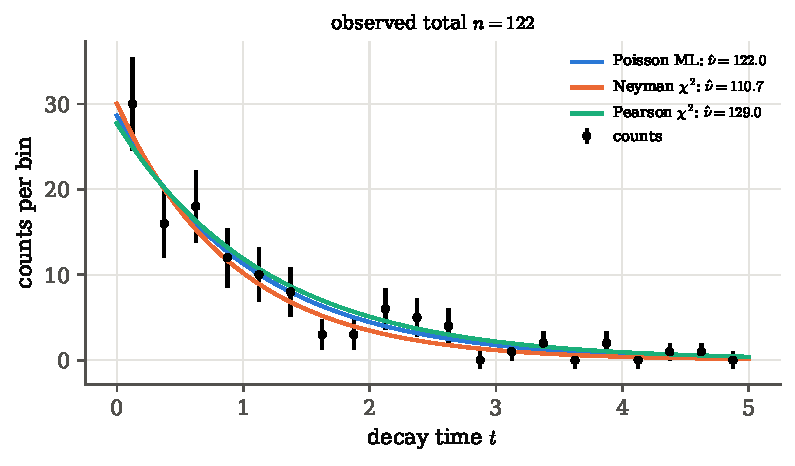
\includegraphics[width=10cm]{figures/ch03/poisson_fit.pdf}
\caption{One histogram of decay times with few counts per bin (points,
with $\sqrt{\max(n_i,1)}$ bars for orientation only) and three fits of the
same exponential shape. The Poisson likelihood fit reproduces the observed
total. The Neyman $\chi^2$ fit sits low, pulled down by the bins that
fluctuated low; the Pearson $\chi^2$ fit sits high.}
\label{3b:fig:poisson-fit}
\end{figure}

Over $3000$ simulated histograms the Poisson fit returns
$|\hat\nu-n|\le\ThreeBPoisDiffP$ in every one of them, the exact
conservation law of \eqref{3b:eq:poisson-split} up to the tolerance of the
minimiser. The Pearson fit is high by $\ThreeBPoisDiffS$ events on average,
exactly $\tfrac12\overline{\chi^2_{P,\min}}=\ThreeBPoisPredS$. The Neyman fit
is low by $\ThreeBPoisDiffN$; the relation $\hat\nu_N=n-\chi^2_{N,\min}$
predicts $\ThreeBPoisPredN$, and the difference is entirely due to the patch
for empty bins, which breaks the identity $\sum_ip_in_i/n_i=1$ used in its
derivation. The bias leaks into the shape: the mean fitted lifetimes are
$\ThreeBPoisTauMeanP$, $\ThreeBPoisTauMeanN$ and $\ThreeBPoisTauMeanS$ for
a true value of $1$. Finally, the Baker--Cousins $\chi^2_{\lambda,\min}$
averages $\ThreeBPoisBCmean$ against $\ThreeBPoisDof$ degrees of freedom
and follows the $\chi^2_{18}$ curve even with this sparse histogram
(\cref{3b:fig:poisson-bias}).

\begin{figure}[htbp]
\centering
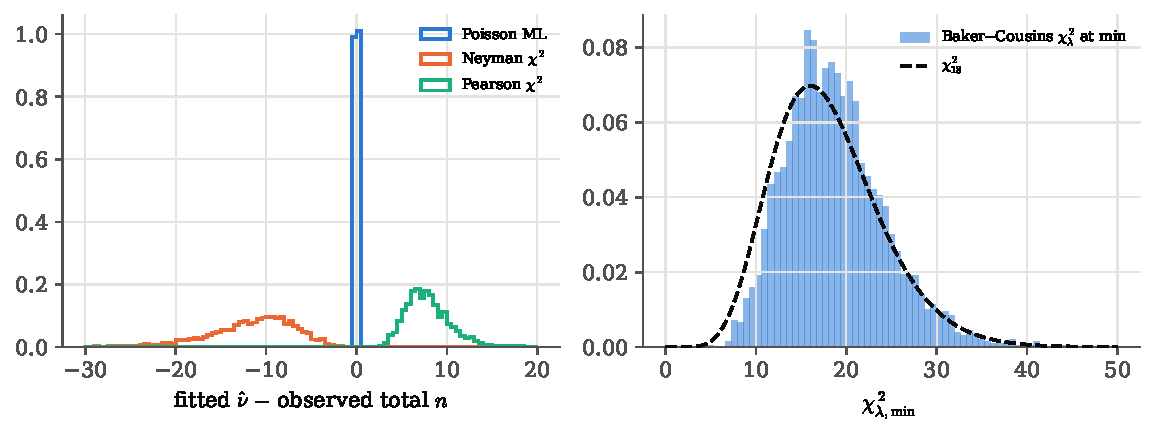
\includegraphics[width=12cm]{figures/ch03/poisson_bias.pdf}
\caption{Three thousand simulated histograms. Left: fitted total minus
observed total. The Poisson fit is a spike at zero; the Neyman fit is
biased low by about ten events and the Pearson fit high by about eight.
Right: the Baker--Cousins statistic at its minimum follows the $\chi^2$
distribution for $20-2=18$ degrees of freedom, so it can be used as a
goodness-of-fit test.}
\label{3b:fig:poisson-bias}
\end{figure}

\subsection{One idea, three implementations}
\label{3b:sec:universal}

The recipe is always the same: write the prediction, write the probability
of the fluctuation needed to turn it into the data, and multiply over
independent pieces. Only the noise model changes from one field to another.
Three noise models cover most data in physics and cosmology: Poisson counts;
Gaussian noise with a covariance that does not depend on the parameters
(gravitational-wave strain is this case written in frequency); and a
Gaussian field whose covariance is itself the signal, as for the CMB.

\begin{taxonomy}[Which likelihood when]
\small
\begin{tabular}{@{}>{\raggedright\arraybackslash}p{3.3cm}>{\raggedright\arraybackslash}p{4.4cm}>{\raggedright\arraybackslash}p{5.0cm}@{}}
  data & noise model & $-2\ln\Like$ (up to constants)\\
  \hline
  counts in bins (colliders, X-ray, decay histograms)
    & $n_i\sim\mathrm{Poisson}(\mu_i(\params))$, independent bins
    & $2\sum_i[\mu_i-n_i\ln\mu_i]$ \eqref{3b:eq:poisson-like}\\[2pt]
  measurements with error bars; binned spectra
    & Gaussian, covariance $\Cmat$ independent of $\params$
    & $\bm r\T\Cmat^{-1}\bm r$ \eqref{3b:eq:like-corr}\\[2pt]
  GW strain
    & stationary Gaussian noise with PSD $S_n(f)$
    & $(D-h_{\params}|D-h_{\params})$ (\cref{3b:sec:correlated})\\[2pt]
  CMB map, full sky, no noise
    & $\alm$ Gaussian with variance $\Cell(\params)$
    & $\sum_\ell(2\ell+1)\bigl[\Chat/\Cell+\ln\Cell\bigr]$\\
\end{tabular}
\end{taxonomy}

The last line needs a derivation, because it is the first case where the
parameters sit in the covariance rather than in the mean. In a statistically
isotropic Gaussian sky the spherical-harmonic coefficients $\alm$ have mean
zero and variance $\Cell$, the theory's power spectrum. The measured
spectrum is $\Chat=\frac{1}{2\ell+1}\sum_m|\alm|^2$. Because the sky is real,
$a_{\ell,-m}$ is fixed by $a_{\ell m}$, so at each $\ell$ there are
$2\ell+1$ independent real numbers: $a_{\ell0}$, and $\sqrt2\,\mathrm{Re}\,\alm$
and $\sqrt2\,\mathrm{Im}\,\alm$ for $m=1,\dots,\ell$. Call them $y_{\ell k}$,
$k=1,\dots,2\ell+1$. Each is Gaussian with variance $\Cell$, and
$\sum_ky_{\ell k}^2=\sum_m|\alm|^2=(2\ell+1)\Chat$. Then
\begin{align*}
  -2\ell(\params)
  &\eqby{1}\sum_\ell\sum_{k=1}^{2\ell+1}\Bigl[\frac{y_{\ell k}^2}{\Cell(\params)}+\ln\Cell(\params)+\ln2\pi\Bigr]
  \eqby{2}\sum_\ell(2\ell+1)\Bigl[\frac{\Chat}{\Cell(\params)}+\ln\Cell(\params)\Bigr]+\text{const}.
\end{align*}
\begin{explain}
  \item \eqref{3b:eq:like-corr} with a diagonal covariance whose entries
        are $\Cell$: $-2\ln$ of each Gaussian factor is
        $y^2/\Cell+\ln\Cell+\ln2\pi$.
  \item Sum over $k$ using $\sum_ky_{\ell k}^2=(2\ell+1)\Chat$; the $2\ell+1$
        copies of $\ln\Cell$ give the second term.
\end{explain}
The $\ln\Cell$ term is the $\ln\det\Cmat$ of \eqref{3b:eq:like-corr}, and it
cannot be dropped: without it the fit would push every $\Cell$ to
infinity. If the model sets each $\Cell$ free, the score equation
$-\Chat/\Cell^2+1/\Cell=0$ gives $\hat C_\ell=\Chat$, so the familiar
estimator is the maximum likelihood estimator. As a function of $\Cell$
this likelihood is skewed, like the Poisson one above, and for the same
reason: the spread of $\Chat$ grows with its mean. A mask, instrument noise
and a beam change this likelihood, as \cref{ch:07,ch:08} show.
\section{The width of the likelihood is the error bar}
\label{3b:sec:curvature}

The width of the likelihood is the error bar of the estimate. To see why
one would expect this, look at a likelihood with a sharp peak. Only a
narrow range of parameter values can turn the prediction into the data
with an ordinary fluctuation. Move a little away and the noise required
becomes implausible. A broad likelihood says the opposite: many values
would have done about equally well. For linear models with Gaussian noise
we proved the claim exactly in \cref{3b:sec:linear-ls}: the log-likelihood
is a parabola whose width is the standard deviation of $\hat\theta$. For any
smooth likelihood with enough data it holds approximately, and a check on
$10^4$ simulated experiments shows how well. Three questions follow.
\begin{enumerate}[label=\arabic*.]
  \item How do we read an error bar off the log-likelihood, from its
        curvature or from where it has dropped by $\tfrac12$?
  \item Why should the width of a function of $\theta$, computed from one
        data set, equal the scatter of $\hat\theta$ over many data sets? The
        answer introduces the Fisher information.
  \item How well does it work at a realistic sample size?
\end{enumerate}

\subsection{Curvature at the peak}
\label{3b:sec:curv-peak}

Expand the log-likelihood about its maximum, where the first derivative
vanishes \srcref{Padilla}{(29)--(31)}:
\begin{align}
  \ell(\theta)
  &\eqby{1}\ell(\hat\theta)+\underbrace{\ell'(\hat\theta)}_{=0}(\theta-\hat\theta)
   +\tfrac12\ell''(\hat\theta)(\theta-\hat\theta)^2+\dots
  \eqby{2}\ell_{\max}-\frac{(\theta-\hat\theta)^2}{2\hat\sigma^2}+\dots,
  \qquad
  \hat\sigma^2\equiv\frac{1}{-\ell''(\hat\theta)} .
  \label{3b:eq:curvature}
\end{align}
\begin{explain}
  \item Taylor's theorem at the maximum; the score vanishes there.
  \item $\ell''(\hat\theta)<0$ at a maximum, so $-1/\ell''$ is positive and
        we may call it $\hat\sigma^2$.
\end{explain}
Near its peak the likelihood is therefore
$\Like(\theta)\approx\Like_{\max}\exp[-(\theta-\hat\theta)^2/2\hat\sigma^2]$,
a Gaussian bump of width $\hat\sigma$. The rule is: \emph{the error bar is
one over the square root of minus the second derivative of $\ln\Like$ at its
maximum} \srcref{Cowan}{\S6.4}. For several parameters, minus the matrix of
second derivatives (the Hessian with a minus sign) plays the role of
$1/\hat\sigma^2$, and its inverse is the estimated covariance matrix. That
is the line \pyname{V = np.linalg.inv(-H)} in the Newton--Raphson fit of
the muon angular distribution (\cref{3b:sec:newton}).

\paragraph{Example: the lifetime.}
For $n$ decay times the maximum likelihood lifetime is $\hat\tau=\bar t$,
and \eqref{3b:eq:tau-mle} gave $-\ell''(\hat\tau)=n/\hat\tau^2$. So
$\hat\sigma_{\hat\tau}=\hat\tau/\sqrt n$. Fifty decays measure a lifetime to
$1/\sqrt{50}\approx14\%$. The true standard deviation of $\bar t$ is
$\tau/\sqrt n$ (\cref{3b:sec:mle-hand}), and the curvature gives the same
formula with the unknown $\tau$ replaced by its estimate.

\paragraph{Example: the detector efficiency.}
For the detector that fires $S$ times in $n$ trials, the log-likelihood is
$\ell(p)=S\ln p+(n-S)\ln(1-p)$ and $\hat p=S/n$ (\cref{3b:sec:mle-hand}).
Then
\begin{align*}
  -\ell''(p)&\eqby{1}\frac{S}{p^2}+\frac{n-S}{(1-p)^2},\qquad
  -\ell''(\hat p)\eqby{2}\frac{n}{\hat p}+\frac{n}{1-\hat p}
  \eqby{3}\frac{n}{\hat p(1-\hat p)},\qquad
  \hat\sigma_{\hat p}=\sqrt{\frac{\hat p(1-\hat p)}{n}} .
\end{align*}
\begin{explain}
  \item Differentiate $S/p-(n-S)/(1-p)$ once more.
  \item At $\hat p=S/n$: $S/\hat p^2=n/\hat p$ and
        $(n-S)/(1-\hat p)^2=n/(1-\hat p)$.
  \item Common denominator: $1/\hat p+1/(1-\hat p)=1/[\hat p(1-\hat p)]$.
\end{explain}
For $S=12$ out of $n=20$ this is $\sqrt{0.6\cdot0.4/20}=0.11$, the
binomial standard error.

\subsection{The graphical method: where \texorpdfstring{$\ln\Like$}{ln L} has dropped by one half}
\label{3b:sec:delta-lnl}

If $\ell$ were exactly the parabola \eqref{3b:eq:curvature}, then at
$\theta=\hat\theta\pm\hat\sigma$ it would be exactly $\ell_{\max}-\tfrac12$.
That suggests a second recipe that does not need derivatives: draw
$\ell(\theta)$ and read off where it crosses $\ell_{\max}-\tfrac12$
\srcref{Cowan}{\S6.7}. For Gaussian data $-2\ell=\chi^2+\text{const}$, so
this is the $\Delta\chi^2=1$ rule of \cref{3b:sec:chi2-min}. When the
log-likelihood is not a parabola, the two crossings are at different
distances from $\hat\theta$, and one quotes an asymmetric error
$\hat\theta^{+\sigma_+}_{-\sigma_-}$.

\paragraph{Example: the lifetime interval exactly.}
Measure $\tau$ in units of the estimate, $u=\tau/\hat\tau$. Using
$T=n\hat\tau$,
\begin{align*}
  \ell(\tau)-\ell(\hat\tau)
  &\eqby{1}-n\ln\tau-\frac{n\hat\tau}{\tau}+n\ln\hat\tau+n
  \eqby{2}-n\Bigl[\ln u+\frac1u-1\Bigr].
\end{align*}
\begin{explain}
  \item $\ell(\tau)=-n\ln\tau-T/\tau$ at $\tau$ and at $\hat\tau$, with
        $T/\hat\tau=n$.
  \item $\ln\tau-\ln\hat\tau=\ln u$ and $\hat\tau/\tau=1/u$.
\end{explain}
The $\Delta\ln\Like=\tfrac12$ interval is the pair of roots of
$\ln u+1/u-1=1/(2n)$, the same for every data set once expressed in units of
$\hat\tau$. For small $u-1$, $\ln u+1/u-1\approx\tfrac12(u-1)^2$, which
returns $u=1\pm1/\sqrt n$, the curvature error. For $n=50$ the exact roots
are $u=0.871$ and $u=1.156$: the interval reaches further up than down,
because decay times drawn with a longer lifetime also scatter more.

\paragraph{Why the graphical interval is the better one.}
The curvature error depends on how we name the parameter; the $\Delta\ln\Like$
interval does not. The likelihood assigns the same number to a hypothesis
whatever we call it (\cref{3b:sec:not-density}). So if we switch from $\tau$
to the rate $\lambda=1/\tau$, the set of hypotheses with
$\ell\ge\ell_{\max}-\tfrac12$ is the same set, merely relabelled. If
$\tau_-$ and $\tau_+$ are the lower and upper ends of the $\tau$ interval,
the $\lambda$ interval is $[1/\tau_+,1/\tau_-]$. The curvature, by contrast,
changes: $-\partial^2\ell/\partial\lambda^2$ at $\hat\lambda$ is $n/\hat\lambda^2$,
so the curvature interval in $\lambda$ is $\hat\lambda(1\pm1/\sqrt n)$,
which is \emph{not} the image of $\hat\tau(1\pm1/\sqrt n)$. The two
symmetric recipes disagree with each other, and each is right only to
leading order. The graphical interval behaves as if we had found and used
the parametrisation in which $\ell$ is most nearly a parabola, without our
having to find it.

\begin{pitfall}[A curvature error assumes a parabola]
$\hat\sigma=(-\ell'')^{-1/2}$ describes the peak only. If $\ell$ is skewed,
has a second maximum, or is cut off by a physical boundary (a mass that
cannot be negative, a cliff like the uniform box), the curvature says
nothing about the tails. Always plot $\ln\Like$, or at least find the two
$\Delta\ln\Like=\tfrac12$ crossings, before quoting $\pm\hat\sigma$.
\end{pitfall}

\paragraph{Several parameters.}
With two parameters the level set $\ell=\ell_{\max}-\tfrac12$ is a closed
curve, an ellipse when $\ell$ is quadratic. In the right panel of
\cref{3b:fig:angular} it is drawn for the fit of the angular distribution
$1+\alpha x+\beta x^2$ (\cref{3b:sec:newton}). The dotted lines tangent to it
are at $\hat\alpha\pm\sigma_{\hat\alpha}$ and $\hat\beta\pm\sigma_{\hat\beta}$,
with the errors from the inverse Hessian \srcref{Cowan}{\S6.8}. Why tangent
lines? Fix $\alpha$ and move $\beta$ to make $\ell$ as large as possible. As
$\alpha$ moves away from $\hat\alpha$ this best value falls, and it reaches
$\ell_{\max}-\tfrac12$ exactly where the vertical line at that $\alpha$
touches the contour. That best value as a function of $\alpha$ is the profile
likelihood of \cref{3b:sec:profile}. The tilt of the ellipse shows the
correlation between the two estimates. For that fit the inverse Hessian gives
$\sigma_{\hat\alpha}=\ThreeBAngSa$, $\sigma_{\hat\beta}=\ThreeBAngSb$ and
$\rho=\ThreeBAngRho$; the $500$ repetitions scatter with
$\ThreeBAngSdA$, $\ThreeBAngSdB$ and $\rho=\ThreeBAngRhoMC$. The standard
deviations agree to a few per cent. The correlation from $500$ pairs is
itself uncertain by $(1-\rho^2)/\sqrt{500}=\ThreeBAngRhoMCErr$, so the two
values of $\rho$ should be compared within that error. The Hessian's own
$\rho$ also changes from one experiment to the next: over the $500$
repetitions it averages $\ThreeBAngRhoHessMean$ and scatters by
$\ThreeBAngRhoHessSd$. Its average and the repetitions' $\rho$ are consistent
within about two of the repetitions' errors: $500$ repetitions are not enough
to tell them apart. The $\tfrac12$-contour projects onto each
axis as a $68\%$ interval for that parameter alone. A region that should
contain \emph{both} true values with $68\%$ probability is the larger
contour $\Delta\ln\Like=2.30/2=1.15$, as in the $\Delta\chi^2$ table of
\cref{3b:sec:chi2-min}.

\subsection{Why the curvature is the error: score and Fisher information}
\label{3b:sec:fisher-info}

We now have a recipe that uses one data set, a second derivative of a
function of $\theta$. The error bar we want is a statement about many data
sets: the standard deviation of $\hat\theta$ over imagined repetitions. Why
should they agree? The bridge is the score, $S(\theta)=\ell'(\theta)$,
viewed as a random variable. For a fixed $\theta$, each data set gives a
different score. Two identities about its distribution do all the work.
They hold whenever we may differentiate under the integral sign, which
requires, in particular, that the range of the data does not depend on
$\theta$ (it fails for the uniform box).

\paragraph{The score has mean zero.} For a single observation with density
$f(x;\theta)$,
\begin{align}
  \E_\theta\Bigl[\frac{\partial\ln f(X;\theta)}{\partial\theta}\Bigr]
  &\eqby{1}\int\frac{\partial_\theta f(x;\theta)}{f(x;\theta)}\,f(x;\theta)\,\dd x
  \eqby{2}\frac{\partial}{\partial\theta}\int f(x;\theta)\,\dd x
  \eqby{3}\frac{\partial}{\partial\theta}1=0 .
  \label{3b:eq:score-mean}
\end{align}
\begin{explain}
  \item Expectation over the density of the data at the \emph{same}
        $\theta$; $\partial_\theta\ln f=\partial_\theta f/f$.
  \item The $f$ cancels. Exchange the derivative and the integral (the
        regularity condition).
  \item Every density integrates to one, for every $\theta$.
\end{explain}
At the true parameter, the data pull neither up nor down on average.

\paragraph{The variance of the score is minus the mean curvature.}
Now differentiate the identity
\[
  \int(\partial_\theta\ln f)\,f\,\dd x=0
\]
once more with respect to $\theta$:
\begin{align}
  0&\eqby{1}\int\Bigl[(\partial^2_\theta\ln f)\,f+(\partial_\theta\ln f)\,\partial_\theta f\Bigr]\dd x
   \eqby{2}\int\Bigl[\partial^2_\theta\ln f+(\partial_\theta\ln f)^2\Bigr]f\,\dd x ,
  \nonumber\\
  I(\theta)&\equiv\E_\theta\bigl[(\partial_\theta\ln f)^2\bigr]
   \eqby{3}-\E_\theta\bigl[\partial^2_\theta\ln f\bigr] .
  \label{3b:eq:fisher-identity}
\end{align}
\begin{explain}
  \item Product rule under the integral.
  \item $\partial_\theta f=(\partial_\theta\ln f)\,f$.
  \item Split the integral. Since the score has mean zero, the first form
        is its variance.
\end{explain}
For $n$ independent observations, $\ell=\sum_i\ln f(x_i;\theta)$ is a sum of
independent terms, so the variance of the total score and the expected
curvature both add: $I_n(\theta)=nI(\theta)$ \mainref{p.~128, Thm.~9.17}.

\begin{workdef}[Fisher information]
The \newterm{Fisher information} in $n$ observations is
\[
  I_n(\theta)=\Var_\theta\bigl[S(\theta)\bigr]=-\E_\theta\bigl[\ell''(\theta)\bigr]=nI(\theta),
\]
the average curvature of the log-likelihood at the true parameter
\mainref{p.~128, Def.~9.16}. The \newterm{observed information}
$-\ell''(\hat\theta)$ is the curvature of the one log-likelihood we have,
at its peak. \emph{Operationally:} differentiate $\ln f$ twice, take minus
its average over the model, multiply by $n$. For several parameters,
$I_{jk}=-\E[\partial_j\partial_k\ell]$ is the \newterm{Fisher matrix}
(\cref{ch:10}).
\end{workdef}

\paragraph{From the score to the scatter of $\hat\theta$.}
Now expand the score equation of one data set about the true value
$\theta$ \mainref{p.~136}:
\begin{align}
  0&\eqby{1}\ell'(\hat\theta)
   \eqby{2}\ell'(\theta)+(\hat\theta-\theta)\,\ell''(\theta)+\dots
  \quad\Longrightarrow\quad
  \hat\theta-\theta\approx\frac{\ell'(\theta)}{-\ell''(\theta)}
  \eqby{3}\frac{\tfrac1{\sqrt n}\,\ell'(\theta)}{\tfrac1{\sqrt n}\,[-\ell''(\theta)]}
  \nonumber\\
  \sqrt n\,(\hat\theta-\theta)
  &\approx\frac{\frac{1}{\sqrt n}\sum_iS_i}{\frac1n\sum_i[-\partial^2_\theta\ln f(x_i;\theta)]}
  \;\relby{4}{\rightsquigarrow}\;\frac{\Normal\bigl(0,I(\theta)\bigr)}{I(\theta)}
  \eqby{5}\Normal\Bigl(0,\frac1{I(\theta)}\Bigr).
  \label{3b:eq:asymptotic}
\end{align}
\begin{explain}
  \item $\hat\theta$ solves the score equation.
  \item Taylor expansion of $\ell'$ about the true value; for large $n$,
        $\hat\theta$ is close to $\theta$ (consistency,
        \cref{3b:sec:properties}) and the dropped terms are smaller.
  \item Multiply numerator and denominator by $1/\sqrt n$ and move one
        $\sqrt n$ to the left.
  \item The numerator is $\sqrt n$ times the average of the $n$ independent
        scores $S_i=\partial_\theta\ln f(x_i;\theta)$, each of mean $0$
        \eqref{3b:eq:score-mean} and variance $I(\theta)$
        \eqref{3b:eq:fisher-identity}, so by the central limit theorem it
        tends to $\Normal(0,I)$. The denominator is an average of $n$
        independent curvatures with mean $I(\theta)$, so by the law of
        large numbers it tends to the constant $I(\theta)$.
  \item Dividing a $\Normal(0,I)$ variable by the number $I$ gives variance
        $I/I^2=1/I$.
\end{explain}
So the scatter of $\hat\theta$ over repetitions is set by the Fisher
information, the \emph{average} curvature of the log-likelihood. The
curvature $-\ell''(\hat\theta)$ of the one data set we have is an average of
$n$ independent curvatures, so by the same law of large numbers it is close
to $I_n$. That is why the width read off our one likelihood gives the error
bar.

\begin{keyidea}[The curvature of $\ln\Like$ is the error bar]
For a regular model and large $n$ the MLE is approximately Gaussian,
\[
  \hat\theta\approx\Normal\Bigl(\theta,\ \frac{1}{I_n(\theta)}\Bigr),\qquad
  \widehat{\mathrm{se}}=\frac{1}{\sqrt{I_n(\hat\theta)}}
  \;\approx\;\frac{1}{\sqrt{-\ell''(\hat\theta)}},
\]
and $\hat\theta\pm1.96\,\widehat{\mathrm{se}}$ is an approximate $95\%$
confidence interval \mainref{pp.~129--130, Thms.~9.18--9.19}. With several
parameters, $\Cov\hat\params\approx I_n^{-1}$.
\end{keyidea}

\paragraph{Examples of Fisher information.}
The standard cases follow from \eqref{3b:eq:fisher-identity} in one line
each \mainref{p.~130, Exs.~9.20--9.22}.
\begin{itemize}
  \item Gaussian mean, known $\sigma$: $\ln f=-(x-\mu)^2/2\sigma^2+\dots$,
        $\partial^2_\mu\ln f=-1/\sigma^2$, so $I=1/\sigma^2$ and
        $\mathrm{se}=\sigma/\sqrt n$. The curvature is the same for every
        data set, so observed and expected information coincide exactly.
  \item Poisson counts, mean $\lambda$: $\ln f=x\ln\lambda-\lambda-\ln x!$,
        $\partial^2_\lambda\ln f=-x/\lambda^2$, and $\E X=\lambda$ gives
        $I=1/\lambda$, $\mathrm{se}=\sqrt{\lambda/n}$.
  \item Bernoulli: $\partial_p^2\ln f=-x/p^2-(1-x)/(1-p)^2$, with
        $\E X=p$, so $I=1/p+1/(1-p)=1/[p(1-p)]$.
  \item Exponential lifetime: $\partial^2_\tau(-\ln\tau-t/\tau)=1/\tau^2-2t/\tau^3$,
        with $\E t=\tau$, so $I=1/\tau^2$ and
        $\mathrm{se}=\tau/\sqrt n$.
\end{itemize}
The information per observation is large where the density changes quickly
as $\theta$ changes, because then each observation discriminates sharply
between nearby values: a Gaussian of small $\sigma$, a Poisson mean near
zero, a coin whose $p$ is near $0$ or $1$.

\subsection{Testing the recipe on \texorpdfstring{$10^4$}{10\^4} experiments}
\label{3b:sec:curv-python}

The script \pyname{09_mle_decay.py} tests the whole argument on the
lifetime, for $n=\ThreeBDecN$ decays with true lifetime $\tau=1$. It first
analyses one experiment, the way an experimenter would.
\pyfile[firstline=32,lastline=40]{code/ch03/09_mle_decay.py}{One experiment: the MLE, the curvature error and the $\Delta\ln\Like=\tfrac12$ interval}
The analytic MLE is the mean; \pyname{minimize_scalar} confirms it
numerically ($\ThreeBDecTauNum$). The curvature error is
$\hat\tau/\sqrt n$. The function \pyname{f} is zero where $\ln\Like$ has
dropped by $\tfrac12$, and \pyname{brentq} finds its two roots on either
side of the peak. The result is
\[
  \hat\tau=\ThreeBDecTauHat\pm\ThreeBDecSigCurv\ \text{(curvature)},\qquad
  \hat\tau=\ThreeBDecTauHat^{+\ThreeBDecHi}_{-\ThreeBDecLo}\ \text{($\Delta\ln\Like=\tfrac12$)} .
\]
\Cref{3b:fig:mle-lnL} shows the log-likelihood and its parabola: close near
the peak, with the curve falling more steeply on the low side.

\begin{figure}[htbp]
\centering
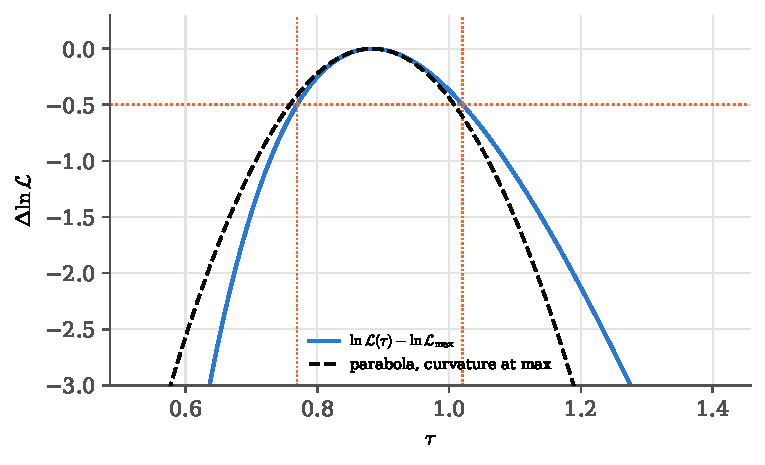
\includegraphics[width=9cm]{figures/ch03/mle_decay_lnL.pdf}
\caption{The log-likelihood of one experiment with fifty decays (solid)
and the parabola with the same curvature at the peak (dashed). The dotted
horizontal line is $\ln\Like_{\max}-\tfrac12$; its crossings with the curve
(dotted verticals) give the asymmetric interval. The curve drops faster than
the parabola on the left and slower on the right.}
\label{3b:fig:mle-lnL}
\end{figure}

Then the script does what no experimenter can: it repeats the experiment
$10^4$ times and looks at the scatter.
\pyfile[firstline=55,lastline=65]{code/ch03/09_mle_decay.py}{Ten thousand experiments: scatter and coverage}
The numbers are
\begin{center}
\small
\begin{tabular}{lc}
  \hline
  quantity & value\\
  \hline
  mean of $\hat\tau$ over $10^4$ experiments & $\ThreeBDecMeanTau$\\
  true scatter of $\hat\tau$ (Monte Carlo) & $\ThreeBDecSdMC$\\
  $1/\sqrt{I_n(\tau)}=\tau/\sqrt n$ & $\ThreeBDecSdTh$\\
  average curvature error $\hat\tau/\sqrt n$ & $\ThreeBDecMeanCurv$\\
  coverage of $\hat\tau\pm\hat\tau/\sqrt n$ & $\ThreeBDecCoverCurv$\\
  coverage of the $\Delta\ln\Like=\tfrac12$ interval & $\ThreeBDecCoverDl$\\
  \hline
\end{tabular}
\end{center}
The scatter of the MLE over repetitions is the inverse square root of the
Fisher information, to within the Monte Carlo error (about $0.7\%$ for
$10^4$ experiments). The curvature error of an individual experiment
fluctuates with $\hat\tau$, as the right panel of \cref{3b:fig:mle-scatter}
shows, but it is correct on average. Both intervals cover the true value in
about $68\%$ of the experiments, the fraction a $\pm1\sigma$ Gaussian
interval should cover ($0.683$). At $n=50$ the asymptotic theory is
already good. The left panel shows that the exact sampling distribution of
$\hat\tau$, a Gamma distribution with shape $n$ (the sum of $n$
exponentials, \cref{ch:02}), is slightly skewed compared with the Gaussian
of \eqref{3b:eq:asymptotic}; the skewness shrinks like $1/\sqrt n$.

\begin{figure}[htbp]
\centering
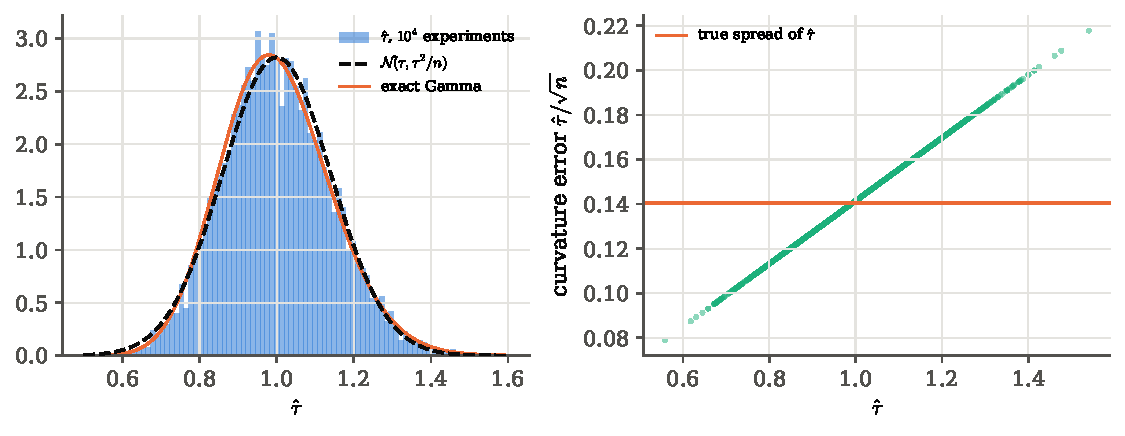
\includegraphics[width=12cm]{figures/ch03/mle_decay_scatter.pdf}
\caption{Ten thousand repetitions of the fifty-decay experiment. Left: the
histogram of the maximum likelihood lifetimes, the Gaussian predicted by the
Fisher information (dashed) and the exact Gamma distribution (solid). Right:
each experiment's curvature error plotted against its estimate. The error
grows with $\hat\tau$, because it is $\hat\tau/\sqrt n$, and it scatters
around the true spread of the estimates (horizontal line).}
\label{3b:fig:mle-scatter}
\end{figure}
\section{What makes maximum likelihood good}
\label{3b:sec:properties}

We now have many ways to turn data into a number: the mean, the median,
the method of moments, least squares, maximum likelihood. Why is maximum
likelihood the default of experimental physics? Not because it is always
unbiased. The Gaussian width $\hat\sigma^2$ is not (\cref{3b:sec:mle-hand}),
and the decay rate $1/\hat\tau$ is not either (\cref{3b:sec:invariance}).
The reason is a set of large-sample properties
\mainref{p.~125}. For a regular model (smooth in $\theta$, with a support
that does not move with $\theta$, and a true value inside the parameter
space) the MLE is
\begin{enumerate}[label=\arabic*.]
  \item \emph{consistent}: it converges to the true value;
  \item \emph{equivariant}: the MLE of $g(\theta)$ is $g(\hat\theta)$;
  \item \emph{asymptotically Gaussian}, with variance $1/I_n(\theta)$
        (\cref{3b:sec:fisher-info});
  \item \emph{asymptotically efficient}: no unbiased estimator has a
        smaller variance than $1/I_n$, so for large $n$ nothing beats it;
  \item \emph{approximately Bayesian}: for large $n$ the posterior with any
        smooth prior peaks near $\hat\theta$ with width $1/\sqrt{I_n}$
        (\cref{ch:05}).
\end{enumerate}
The third is \eqref{3b:eq:asymptotic}. Each of the first, second and fourth
has a short reason, each can be seen working on simulated data, and each
fails when one of the regularity conditions fails.

\subsection{Consistency: the log-likelihood peaks at the truth}
\label{3b:sec:consistency}

Why should the peak of the likelihood of one finite data set sit near the
true value $\theta_\star$? The answer is that, as $n$ grows, the
log-likelihood per observation settles down to a fixed curve, and that
curve peaks at $\theta_\star$. To see it, compare each $\theta$ with the
truth through the average log-likelihood ratio
\[
  M_n(\theta)=\frac1n\sum_{i=1}^n\ln\frac{f(x_i;\theta)}{f(x_i;\theta_\star)} .
\]
It differs from $\ell(\theta)/n$ only by a term that does not depend on
$\theta$, so it peaks at $\hat\theta$. It is an average of $n$ independent
terms, so by the law of large numbers it approaches its expectation,
\begin{align}
  M_n(\theta)\;\to\;\E_{\theta_\star}\!\Bigl[\ln\frac{f(X;\theta)}{f(X;\theta_\star)}\Bigr]
  &\eqby{1}-\int f(x;\theta_\star)\ln\frac{f(x;\theta_\star)}{f(x;\theta)}\,\dd x
  \equiv-D(\theta_\star,\theta),
  \label{3b:eq:kl}
\end{align}
\begin{explain}
  \item Write the expectation as an integral over the true density and flip
        the ratio inside the logarithm, which flips the sign.
\end{explain}
where $D(f,g)=\int f\ln(f/g)$ is the \newterm{Kullback--Leibler divergence}
\unpack{how badly the density $g$ describes data that really come from $f$,
in units of log-probability per observation} \mainref{p.~126}. It is never
negative, and it vanishes only when the two densities are equal:
\begin{align*}
  -D(f,g)
  &\eqby{1}\E_f\Bigl[\ln\frac{g(X)}{f(X)}\Bigr]
  \relby{2}{\le}\ln\E_f\Bigl[\frac{g(X)}{f(X)}\Bigr]
  \eqby{3}\ln\int f(x)\frac{g(x)}{f(x)}\,\dd x
  \eqby{4}\ln 1=0 .
\end{align*}
\begin{explain}
  \item Definition of $D$ with the ratio inverted.
  \item Jensen's inequality: $\ln$ is concave, so the average of the
        logarithm is at most the logarithm of the average, with equality only
        if $g/f$ is constant.
  \item Expectation over $f$.
  \item $g$ is a density and integrates to one. A constant ratio $g/f$
        must therefore equal one.
\end{explain}
Physicists know this as the Gibbs inequality of statistical mechanics:
relative entropy is non-negative. So the limit of $M_n$ is a function with a
unique maximum, equal to zero, at $\theta=\theta_\star$, provided different
parameter values give different densities (the model is
\newterm{identifiable}). The $M_n$ curves converge to that function, and
their peaks, which are the MLEs, converge to its peak. That is Wasserman's
consistency theorem \mainref{p.~127, Thm.~9.13}; the proof needs the
convergence to hold uniformly in $\theta$, which is where regularity
conditions enter.

\paragraph{Example: the lifetime.}
For exponential decays,
\begin{align*}
  D(\tau_\star,\tau)
  &\eqby{1}\E_{\tau_\star}\Bigl[\ln\frac{\tau_\star^{-1}e^{-t/\tau_\star}}{\tau^{-1}e^{-t/\tau}}\Bigr]
  \eqby{2}\ln\frac{\tau}{\tau_\star}+\E_{\tau_\star}[t]\Bigl(\frac1\tau-\frac1{\tau_\star}\Bigr)
  \eqby{3}\ln\frac{\tau}{\tau_\star}+\frac{\tau_\star}{\tau}-1 .
\end{align*}
\begin{explain}
  \item Definition \eqref{3b:eq:kl} with the exponential density.
  \item $\ln$ of the ratio is $\ln(\tau/\tau_\star)-t/\tau_\star+t/\tau$;
        take the expectation term by term.
  \item $\E_{\tau_\star}t=\tau_\star$.
\end{explain}
This is the same function $\ln u+1/u-1$ that appeared in the exact
$\Delta\ln\Like$ interval, now with $u=\tau/\tau_\star$: the expected shape
of the log-likelihood, per event, is minus the Kullback--Leibler divergence.
The script \pyname{13_efficiency.py} draws $M_n(\tau)$ for one data set each
of $n=10$, $100$ and $1000$ decays (\cref{3b:fig:consistency}). Their peaks,
the MLEs, are at $\ThreeBConsTen$, $\ThreeBConsHund$ and $\ThreeBConsThou$,
and the curves close in on $-D(\tau_\star,\tau)$ as $n$ grows.

\begin{figure}[htbp]
\centering
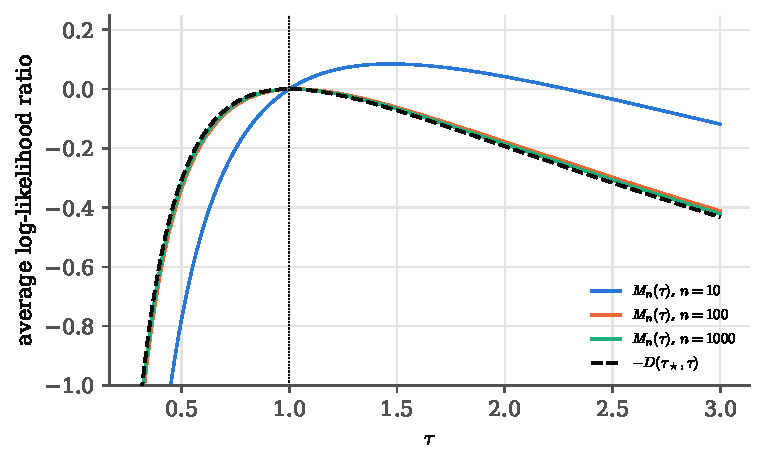
\includegraphics[width=9cm]{figures/ch03/consistency_kl.pdf}
\caption{Why the MLE is consistent. The average log-likelihood ratio
$M_n(\tau)$ of one simulated data set, for $10$, $100$ and $1000$ decays,
approaches minus the Kullback--Leibler divergence (dashed), which has its
maximum, zero, exactly at the true lifetime (dotted). The peak of each
$M_n$ is that data set's MLE, and it is dragged towards the truth as the
curves converge.}
\label{3b:fig:consistency}
\end{figure}

The same argument says what happens when the model is wrong. If the data
come from a density $g$ that is not in the family $f(x;\theta)$, $M_n$ still
converges, now to $-D(g,f(\cdot;\theta))$ plus a constant, and the MLE
converges to the parameter whose density is closest to the truth in the
Kullback--Leibler sense. The fit converges, but to the best wrong answer.

\subsection{Invariance: the MLE does not care what we call the parameter}
\label{3b:sec:invariance}

If $\eta=g(\theta)$ is a one-to-one reparametrisation, the likelihood in
terms of $\eta$ is $\Like^*(\eta)=\Like(g^{-1}(\eta))$: the same numbers
attached to the same hypotheses (\cref{3b:sec:not-density}). Its maximum is
therefore at the $\eta$ that corresponds to $\hat\theta$,
\[
  \hat\eta=g(\hat\theta)
\]
\mainref{p.~127, Thm.~9.14}, \srcref{CasellaBerger}{Thm.~7.2.10}. For a $g$
that is not one-to-one (say $\eta=\theta^2$), Casella and Berger define the
likelihood of $\eta$ as the largest $\Like(\theta)$ over all $\theta$ with
$g(\theta)=\eta$, and the statement still holds. The MLE of the decay rate
is $1/\hat\tau$, the MLE of $\sigma$ is $\sqrt{\hat\sigma^2}$, and the MLE
of the Hubble time is $1/\hat H_0$.

Unbiasedness does not survive such a change. Take $\hat\lambda=1/\hat\tau=n/T$
with $T=\sum_it_i$, a sum of $n$ exponentials, which has the Gamma density
$T^{n-1}e^{-T/\tau}/[\Gamma(n)\tau^n]$ (\cref{ch:02}). Then
\begin{align*}
  \E\Bigl[\frac1T\Bigr]
  &\eqby{1}\int_0^\infty\frac1T\,\frac{T^{n-1}e^{-T/\tau}}{\Gamma(n)\tau^n}\,\dd T
  \eqby{2}\frac{\Gamma(n-1)\,\tau^{n-1}}{\Gamma(n)\,\tau^n}
  \eqby{3}\frac{1}{(n-1)\tau},
  \qquad
  \E\hat\lambda=\frac{n}{n-1}\,\lambda .
\end{align*}
\begin{explain}
  \item Expectation of $1/T$ over the Gamma density.
  \item The remaining integrand is an unnormalised Gamma density of shape
        $n-1$, and
        $\int_0^\infty T^{n-2}e^{-T/\tau}\dd T=\Gamma(n-1)\,\tau^{n-1}$.
  \item $\Gamma(n)=(n-1)\Gamma(n-1)$.
\end{explain}
For $n=50$ the bias factor is $50/49=\ThreeBDecLamTh$; the $10^4$
experiments of \pyname{09_mle_decay.py} give $\E\hat\lambda=\ThreeBDecLamMean$.
Since $\hat\tau$ is exactly unbiased, $\hat\lambda$ cannot be. A nonlinear
function of an unbiased estimator is biased, by Jensen's inequality, just
as the sample standard deviation $S$ is biased for $\sigma$ even though
$S^2$ is unbiased for $\sigma^2$ (\cref{3a:sec:n-minus-one}). So an
estimator can be unbiased in one parametrisation only. Maximum likelihood
gives up unbiasedness and gains consistency in every parametrisation at
once.

The error bar of $\hat\eta=g(\hat\theta)$ follows from the delta method
(\cref{3a:sec:delta}), now applied to the MLE \mainref{p.~131, Thm.~9.24}:
$\widehat{\mathrm{se}}(\hat\eta)\approx|g'(\hat\theta)|\,\widehat{\mathrm{se}}(\hat\theta)$.
For $\lambda=1/\tau$, $|g'|=1/\tau^2$ and
$\widehat{\mathrm{se}}(\hat\lambda)=\hat\tau^{-2}\cdot\hat\tau/\sqrt n=\hat\lambda/\sqrt n$,
the same relative error, as it must be to first order. With several
parameters the gradient replaces the derivative,
$\widehat{\mathrm{se}}^2(\hat\eta)\approx\nabla g\T\,\widehat{\Cov}(\hat\params)\,\nabla g$,
with the covariance from the inverse Fisher matrix
\mainref{p.~134, Thm.~9.28}. For example, take the coefficient of variation
$\eta=\sigma/\mu$ of Gaussian data. One observation has
$\ln f=-\ln\sigma-(x-\mu)^2/2\sigma^2+\text{const}$. Its second derivatives
are $\partial^2_\mu\ln f=-1/\sigma^2$, $\partial_\mu\partial_\sigma\ln
f=-2(x-\mu)/\sigma^3$ and $\partial^2_\sigma\ln f=1/\sigma^2-3(x-\mu)^2/\sigma^4$.
Averaging with $\E(x-\mu)=0$ and $\E(x-\mu)^2=\sigma^2$ and multiplying by
$-n$ gives a diagonal Fisher matrix with entries $n/\sigma^2$ and
$2n/\sigma^2$, so $\Var\hat\mu\approx\sigma^2/n$ and
$\Var\hat\sigma\approx\sigma^2/2n$. The gradient of $\eta$ is
$(\partial_\mu\eta,\partial_\sigma\eta)=(-\sigma/\mu^2,\,1/\mu)$. Then
$\widehat{\mathrm{se}}^2(\hat\eta)=\frac{\hat\sigma^2}{\hat\mu^4}\frac{\hat\sigma^2}{n}
+\frac{1}{\hat\mu^2}\frac{\hat\sigma^2}{2n}
=\hat\sigma^2/(n\hat\mu^2)\,[\hat\sigma^2/\hat\mu^2+\tfrac12]$
\mainref{p.~134, Ex.~9.29}.

\subsection{The Cram\'er--Rao bound: nobody can beat the information}
\label{3b:sec:cramer-rao}

The MLE has asymptotic variance $1/I_n(\theta)$. Could a cleverer
estimator do better? The \newterm{Cram\'er--Rao inequality} (also called
the Rao--Cram\'er--Fr\'echet bound) says no, for any unbiased estimator,
at any sample size \srcref{CasellaBerger}{Thm.~7.3.9}, \srcref{Cowan}{\S6.6}.
The proof is a single use of the Cauchy--Schwarz inequality for
covariances, $\Cov(A,B)^2\le\Var A\,\Var B$, applied to the estimator and
the score.

Let $T(\data)$ be any estimator with mean $m(\theta)=\E_\theta T$, and
$S(\theta)=\partial_\theta\ln p(\data\given\theta)$ the score of the whole
data set. Then
\begin{align}
  \Cov_\theta(T,S)
  &\eqby{1}\E_\theta[T\,S]
  \eqby{2}\int T(\data)\,\frac{\partial_\theta p(\data\given\theta)}{p(\data\given\theta)}\,p(\data\given\theta)\,\dd\data
  \eqby{3}\frac{\partial}{\partial\theta}\int T(\data)\,p(\data\given\theta)\,\dd\data
  \eqby{4}m'(\theta),
  \nonumber\\
  m'(\theta)^2
  &\relby{5}{\le}\Var_\theta T\cdot\Var_\theta S
  \eqby{6}\Var_\theta T\cdot I_n(\theta)
  \quad\Longrightarrow\quad
  \Var_\theta T\;\ge\;\frac{m'(\theta)^2}{I_n(\theta)} .
  \label{3b:eq:cramer-rao}
\end{align}
\begin{explain}
  \item $\Cov(T,S)=\E[TS]-\E T\,\E S$, and $\E S=0$ by \eqref{3b:eq:score-mean}.
  \item Write out the expectation; $S=\partial_\theta p/p$.
  \item Cancel $p$ and move the derivative outside. $T$ depends on the data
        only, not on $\theta$. This exchange is the regularity condition.
  \item The integral is the definition of $m(\theta)$.
  \item Cauchy--Schwarz for covariances, with step (4) on the left.
  \item $\Var S=I_n$, \eqref{3b:eq:fisher-identity}.
\end{explain}
For an unbiased estimator $m(\theta)=\theta$ and $m'=1$, so that
$\Var T\ge1/I_n(\theta)$, which for independent, identically distributed
data is $1/[nI(\theta)]$ \srcref{CasellaBerger}{Cor.~7.3.10}.
If $T$ has a bias $b(\theta)$, then $m=\theta+b$ and the bound is
$(1+b')^2/I_n$, Cowan's form of the inequality.

\begin{keyidea}[Cram\'er--Rao]
For a regular model, every unbiased estimator satisfies
\[
  \Var_\theta\hat\theta\;\ge\;\frac{1}{I_n(\theta)}=\frac{1}{nI(\theta)} .
\]
The Fisher information is the best precision the data can possibly give.
The MLE reaches the bound as $n\to\infty$; it is
\newterm{asymptotically efficient}. For several parameters,
$\Cov\hat\params-\Fish^{-1}$ is positive semidefinite, where $\Fish$ is the
Fisher matrix (\cref{ch:10}).
\end{keyidea}

\paragraph{When is the bound reached exactly?}
Cauchy--Schwarz is an equality only when the two variables are linearly
related. The bound is attained by an unbiased $T$ exactly when
$S(\theta)=a(\theta)\,[T(\data)-\theta]$ for some function $a$
\srcref{CasellaBerger}{Cor.~7.3.15}. This happens for the exponential
families of distributions \mainref{p.~141}. The lifetime is an example: its
score, $-n/\tau+T/\tau^2=(n/\tau^2)(\bar t-\tau)$, has exactly this form,
so $\bar t$ attains the bound $\tau^2/n$ at every $n$, not only
asymptotically. So does $\bar x$ for a Gaussian mean. For the Gaussian
variance with unknown mean the bound is $2\sigma^4/n$, while the best
unbiased estimator, $S^2$, has variance $2\sigma^4/(n-1)$: close, but the
bound is not attained \srcref{CasellaBerger}{Ex.~7.3.14}.

\paragraph{When the bound does not apply: the uniform box again.}
For $\mathrm{Uniform}(0,\theta)$, a blind application of the recipe gives
$\partial_\theta\ln(1/\theta)=-1/\theta$, ``information'' $1/\theta^2$ per
point, and a ``bound'' $\theta^2/n$. But the unbiased estimator
$\tfrac{n+1}{n}x_{(n)}$ does far better. Since
$\Prob(x_{(n)}\le y)=(y/\theta)^n$, the scaled maximum $y=x_{(n)}/\theta$
has density $ny^{n-1}$ on $[0,1]$, and
\begin{align*}
  \E y&\eqby{1}\frac{n}{n+1},\qquad
  \E y^2\eqby{2}\frac{n}{n+2},\\
  \Var\Bigl[\frac{n+1}{n}x_{(n)}\Bigr]
  &\eqby{3}\frac{(n+1)^2}{n^2}\,\theta^2\Bigl[\frac{n}{n+2}-\frac{n^2}{(n+1)^2}\Bigr]
  \eqby{4}\frac{\theta^2}{n(n+2)} .
\end{align*}
\begin{explain}
  \item $\int_0^1y\cdot ny^{n-1}\dd y=n/(n+1)$.
  \item $\int_0^1y^2\cdot ny^{n-1}\dd y=n/(n+2)$.
  \item $\Var(cX)=c^2\Var X$ with $x_{(n)}=\theta y$, and
        $\Var y=\E y^2-(\E y)^2$.
  \item Common denominator:
        $n(n+1)^2-n^2(n+2)=n$, so the bracket is $n/[(n+1)^2(n+2)]$.
\end{explain}
The variance falls like $1/n^2$, not $1/n$. The simulation in
\pyname{13_efficiency.py} gives $n\Var/\theta^2=\ThreeBEffUnifFifty$ at
$n=\ThreeBEffNFifty$, against the exact $1/(n+2)=\ThreeBEffUnifFiftyTh$ and
the ``bound'' $1$. There is no contradiction. Step (3) of
\eqref{3b:eq:cramer-rao} moved a derivative through an integral. Here the
upper limit of that integral is $\theta$ itself, so differentiating it
produces an extra boundary term and the exchange is not allowed. Indeed the
``score'' $-n/\theta$ does not have mean zero: it is not random at all
\srcref{CasellaBerger}{Ex.~7.3.13}. The lesson is that a sharp edge in the
data is worth more than any smooth feature, because a single point near the
edge pins it down. Physicists use this all the time: the endpoint of a
beta spectrum or of a kinematic distribution measures a mass far more
sharply than the bulk of the distribution does.

\subsection{Efficiency in practice: the mean against the median}
\label{3b:sec:efficiency}

The ratio of the variances of two consistent estimators, at large $n$, is
their \newterm{asymptotic relative efficiency}
\mainref{p.~131, Thm.~9.23}. For Gaussian data the mean is the MLE of the
centre and attains the bound $\sigma^2/n$. The sample median also estimates
the centre, and it is popular because a single wild point cannot move it
much. How much precision does it cost?

The asymptotic variance of the median follows from a counting argument. Let
$m$ be the true median and $f(m)$ the density there. The sample median lies
below $m+\delta$ exactly when at least half the points do. The number of
points below $m+\delta$ is binomial with $n$ trials and success probability
$F(m+\delta)\approx\tfrac12+f(m)\delta$, so
\begin{align*}
  \Prob(\hat m\le m+\delta)
  &\eqby{1}\Prob\Bigl(\mathrm{Bin}\bigl(n,\tfrac12+f\delta\bigr)\ge\tfrac n2\Bigr)
  \eqby{2}\Prob\Bigl(Z\ge\frac{n/2-n/2-nf\delta}{\sqrt n/2}\Bigr)
  \eqby{3}\Phi\bigl(2\sqrt n\,f(m)\,\delta\bigr),\\
  \Var\hat m&\eqby{4}\frac{1}{4nf(m)^2}
  \eqby{5}\frac{\pi\sigma^2}{2n}\quad\text{(Gaussian data)}.
\end{align*}
\begin{explain}
  \item The median is below $m+\delta$ if at least $n/2$ points are.
        Near $m$, $F(m+\delta)\approx F(m)+f(m)\delta$ with $F(m)=\tfrac12$.
  \item Gaussian approximation of the binomial (\cref{ch:02}): mean
        $n(\tfrac12+f\delta)$, variance $\approx n/4$ for small $\delta$.
  \item $\Prob(Z\ge-a)=\Phi(a)$ for a standard Gaussian $Z$.
  \item Step (3) says $\hat m-m$ is Gaussian with standard deviation
        $1/(2\sqrt nf)$.
  \item For $\Normal(\mu,\sigma^2)$, $f(m)=1/(\sqrt{2\pi}\sigma)$ and
        $1/(4f^2)=2\pi\sigma^2/4$.
\end{explain}
The median's relative efficiency is $(\sigma^2/n)/(\pi\sigma^2/2n)=2/\pi=0.64$:
using the median on Gaussian data is like throwing away $36\%$ of the
events \mainref{p.~131}. The simulation, $60\,000$ data sets at each of
several $n$, confirms it (\cref{3b:fig:efficiency}): at $n=\ThreeBEffNBig$,
$n\Var$ is $\ThreeBEffMeanBig\,\sigma^2$ for the mean and
$\ThreeBEffMedBig\,\sigma^2$ for the median ($\pi/2=1.571$), an efficiency of
$\ThreeBEffARE$ against $2/\pi=\ThreeBEffAREth$.

\begin{figure}[htbp]
\centering
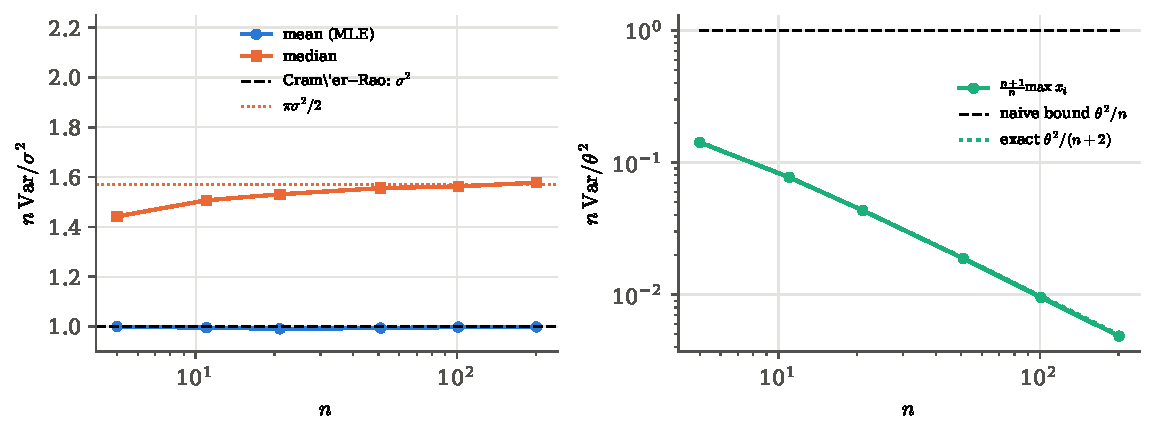
\includegraphics[width=12cm]{figures/ch03/efficiency.pdf}
\caption{Efficiency, simulated. Left: $n$ times the variance of the mean
(the MLE) and of the median for Gaussian data. The mean sits on the
Cram\'er--Rao bound at every $n$; the median approaches $\pi\sigma^2/2$
(dotted). Right: for the uniform box the estimator $\frac{n+1}{n}\max x_i$
falls far below the naive ``bound'' $\theta^2/n$ (dashed) and follows the
exact $\theta^2/(n+2)$ (dotted), because the regularity conditions fail.}
\label{3b:fig:efficiency}
\end{figure}

The lost precision buys robustness. For the Cauchy distribution, whose
tails are so heavy that the sample mean does not converge at all, the
median is consistent, with variance $\pi^2\gamma^2/(4n)$ for half-width
$\gamma$ (the same formula with $f(m)=1/(\pi\gamma)$). The MLE is optimal
only \emph{within the model}. When the real data have heavier tails than the
model allows, an estimator that is slightly inefficient under the model but
robust to outliers can be far better in practice.

\begin{pitfall}[The fine print of ``the MLE is optimal'']
Every property above is asymptotic and assumes a regular model
with the true value inside the parameter space. At small $n$ the MLE can be
biased ($\hat\sigma^2$, $\hat\lambda$). At a boundary (a signal strength
fitted to zero) the sampling distribution is not Gaussian. With a moving
support (the uniform box) the Cram\'er--Rao bound does not apply. When the
number of nuisance parameters grows with the data (one unknown mean per
pair of measurements, say), the MLE of the common parameter need not even be
consistent. Check with a simulation whenever any of these apply.
\end{pitfall}
\section{Nuisance parameters and the profile likelihood}
\label{3b:sec:profile}

Almost no real likelihood has only the parameters we care about. A search
for a new particle wants the signal rate, but the background rate is also
unknown. A cosmological fit wants $\Omega_m$ and $\sigma_8$, but the galaxy
bias, the calibration of the telescope and the amplitude of a foreground
come along. These are \newterm{nuisance parameters}
\unpack{parameters that the likelihood depends on and the data constrain,
but whose values we do not want to report} \mainref{p.~120}. They cannot
be ignored. Fixing them at a guessed value pretends we know them, and that
makes the error on the interesting parameter too small. Three questions
need answers.
\begin{enumerate}[label=\arabic*.]
  \item How do we reduce a likelihood of several parameters to a function
        of the one we care about, without pretending the others are known?
  \item Why does the honest answer have a wider interval, and by how much?
  \item How does this compare with the Bayesian way of removing a nuisance
        parameter, by integrating it out?
\end{enumerate}

\subsection{A signal on top of a background}
\label{3b:sec:on-off}

A standard counting experiment has two regions. In the \emph{signal
region} we count $n_{\text{on}}$ events, expected to be $s+b$: signal plus
background. In a \emph{control region}, chosen so that it contains no
signal, we count $n_{\text{off}}$ events, expected to be $kb$, where the
known factor $k$ is the ratio of exposures (here $k=1$). Both counts are
Poisson, and they are independent:
\[
  \ell(s,b)=n_{\text{on}}\ln(s+b)-(s+b)+n_{\text{off}}\ln(kb)-kb .
\]
The global maximum is easy. Setting the derivatives with respect to $s$
and to $b$ to zero gives the two score equations
$n_{\text{on}}/(s+b)=1$ and $n_{\text{on}}/(s+b)-1+n_{\text{off}}/b-k=0$.
By the first, the first two terms of the second cancel, which leaves
$n_{\text{off}}/b=k$. So $\hat b=n_{\text{off}}/k$, and then the first gives
$\hat s=n_{\text{on}}-n_{\text{off}}/k$. With
$n_{\text{on}}=\ThreeBProfNon$ and $n_{\text{off}}=\ThreeBProfNoff$,
$\hat s=\ThreeBProfS$ and $\hat b=\ThreeBProfB$. The question is the error
on $\hat s$.

\paragraph{Two ways to get a one-dimensional likelihood.}
To get the error on $\hat s$ we need a likelihood of $s$ alone, and there
are two ways to remove $b$. The lazy way is to fix $b$ at its best value
$\hat b$ and look at $\ell(s,\hat b)$, the \newterm{conditional}
likelihood. It pretends that the control region measured $b$ perfectly. The
honest way is to let $b$ adjust: for each trial value of $s$, find the
background that makes the data most probable, and use that.

\begin{workdef}[profile likelihood]
For parameters $(\theta,\bm\nu)$, with $\theta$ of interest and $\bm\nu$
nuisance, the \newterm{profile likelihood} is
\[
  \Like_p(\theta)=\max_{\bm\nu}\Like(\theta,\bm\nu)
  =\Like\bigl(\theta,\hat{\hat{\bm\nu}}(\theta)\bigr),
\]
where $\hat{\hat{\bm\nu}}(\theta)$ is the best value of the nuisance
parameters at fixed $\theta$ \unpack{the ridge line of the likelihood, one
point for every $\theta$}. \emph{Operationally:} on a grid of $\theta$,
maximise over everything else, record the maximum; then treat $\Like_p$ like
a one-parameter likelihood, with its maximum at the global $\hat\theta$.
\end{workdef}

For the on/off problem the inner maximisation can be done by hand. At fixed
$s$,
\begin{align*}
  0&\eqby{1}\frac{n_{\text{on}}}{s+b}-1+\frac{n_{\text{off}}}{b}-k\\
   &\eqby{2}\Rightarrow\ n_{\text{on}}\,b-b(s+b)+n_{\text{off}}(s+b)-kb(s+b)=0\\
   &\eqby{3}\Rightarrow\ (1+k)\,b^2+\bigl[(1+k)s-n_{\text{on}}-n_{\text{off}}\bigr]\,b-n_{\text{off}}\,s=0,
\end{align*}
\begin{explain}
  \item $\partial\ell/\partial b$ at fixed $s$.
  \item Multiply by $b(s+b)>0$.
  \item Collect powers of $b$ and multiply by $-1$.
\end{explain}
and $\hat{\hat b}(s)$ is the positive root of this quadratic (the constant
term is negative for $s>0$, so there is exactly one). As $s$ increases, the
best background decreases: more of the $n_{\text{on}}$ events are already
explained by signal. That anticorrelation is what the conditional likelihood
ignores.

\subsection{Why profiling widens the interval}
\label{3b:sec:profile-width}

Near the maximum every smooth log-likelihood is quadratic, so it is enough
to understand the Gaussian case. Take one parameter of interest $\theta$
and one nuisance parameter $\nu$. Write $\bm x=(\theta-\hat\theta,\nu-\hat\nu)$
and $\ell=\ell_{\max}-\tfrac12\bm x\T\Fish\bm x$ with the information matrix
$\Fish=\begin{pmatrix}F_{\theta\theta}&F_{\theta\nu}\\F_{\theta\nu}&F_{\nu\nu}\end{pmatrix}$,
whose inverse $V=\Fish^{-1}$ is the covariance matrix. Maximise over the
nuisance direction:
\begin{align}
  \ell-\ell_{\max}
  &\eqby{1}-\tfrac12\bigl[F_{\theta\theta}x_\theta^2+2F_{\theta\nu}x_\theta x_\nu+F_{\nu\nu}x_\nu^2\bigr],
  \nonumber\\
  \frac{\partial\ell}{\partial x_\nu}=0
  &\eqby{2}\Rightarrow\ x_\nu=-\frac{F_{\theta\nu}}{F_{\nu\nu}}\,x_\theta ,
  \nonumber\\
  \ell_p-\ell_{\max}
  &\eqby{3}-\tfrac12\Bigl(F_{\theta\theta}-\frac{F_{\theta\nu}^2}{F_{\nu\nu}}\Bigr)x_\theta^2
  \eqby{4}-\frac{x_\theta^2}{2V_{\theta\theta}} .
  \label{3b:eq:profile-gauss}
\end{align}
\begin{explain}
  \item Write out the quadratic form.
  \item Derivative in $x_\nu$: $-(F_{\theta\nu}x_\theta+F_{\nu\nu}x_\nu)=0$.
        This is the profile path, a straight line through the maximum.
  \item Substitute:
        $2F_{\theta\nu}x_\theta x_\nu+F_{\nu\nu}x_\nu^2=-F_{\theta\nu}^2x_\theta^2/F_{\nu\nu}$.
  \item The $(\theta,\theta)$ element of the inverse of a symmetric
        $2\times2$ matrix is
        $V_{\theta\theta}=F_{\nu\nu}/\det\Fish$, and
        $F_{\theta\theta}-F_{\theta\nu}^2/F_{\nu\nu}=\det\Fish/F_{\nu\nu}=1/V_{\theta\theta}$.
\end{explain}
The profile likelihood is a Gaussian of variance $V_{\theta\theta}$: the
full marginal variance of $\hat\theta$, including the uncertainty it
inherits from the nuisance parameter. The conditional likelihood at
$\nu=\hat\nu$ has curvature $F_{\theta\theta}$, hence variance
$1/F_{\theta\theta}$, and
\[
  \frac{1}{F_{\theta\theta}}=V_{\theta\theta}\,(1-\rho^2)\;\le\;V_{\theta\theta},
\]
where $\rho$ is the correlation coefficient of $\hat\theta$ and $\hat\nu$.
The identity follows from the same $2\times2$ inverse, whose entries are
$V_{\theta\theta}=F_{\nu\nu}/\det\Fish$, $V_{\nu\nu}=F_{\theta\theta}/\det\Fish$
and $V_{\theta\nu}=-F_{\theta\nu}/\det\Fish$:
\[
  \rho^2=\frac{V_{\theta\nu}^2}{V_{\theta\theta}V_{\nu\nu}}
        =\frac{F_{\theta\nu}^2}{F_{\theta\theta}F_{\nu\nu}},
  \qquad
  V_{\theta\theta}(1-\rho^2)
  =\frac{F_{\nu\nu}}{\det\Fish}\cdot\frac{F_{\theta\theta}F_{\nu\nu}-F_{\theta\nu}^2}{F_{\theta\theta}F_{\nu\nu}}
  =\frac{1}{F_{\theta\theta}} .
\]
So the conditional interval is too short by the factor $\sqrt{1-\rho^2}$.
The stronger the correlation, the more it understates the error.
\Cref{3b:fig:profile-geometry} shows the geometry.

\begin{figure}[htbp]
\centering
\begin{tikzpicture}[scale=2.0]
  \draw[->,faint] (-1.45,0) -- (1.55,0) node[right,font=\footnotesize,black] {$\theta-\hat\theta$};
  \draw[->,faint] (0,-1.25) -- (0,1.3) node[above,font=\footnotesize,black] {$\nu-\hat\nu$};
  \draw[form,smooth,samples=100,domain=0:360,variable=\t]
    plot ({cos(\t)},{0.6*cos(\t)+0.8*sin(\t)});
  \draw[fibre] (-1.35,-0.81) -- (1.35,0.81);
  \draw[tangentgreen,thick,dashed] (-1.35,0) -- (1.35,0);
  \draw[fibreorange,densely dotted] (1,-1.15) -- (1,1.15);
  \draw[fibreorange,densely dotted] (-1,-1.15) -- (-1,1.15);
  \fill[fibreorange] (1,0.6) circle (1.2pt);
  \fill[fibreorange] (-1,-0.6) circle (1.2pt);
  \fill[tangentgreen] (0.8,0) circle (1.2pt);
  \fill[tangentgreen] (-0.8,0) circle (1.2pt);
  \fill (0,0) circle (1pt);
  \draw[fibreorange,thick,|-|] (-1,-1.45) -- (1,-1.45);
  \node[font=\footnotesize,anchor=west,fibreorange] at (1.05,-1.45) {profile: $\pm\sqrt{V_{\theta\theta}}$};
  \draw[tangentgreen,thick,|-|] (-0.8,-1.65) -- (0.8,-1.65);
  \node[font=\footnotesize,anchor=west,tangentgreen!70!black] at (1.05,-1.65) {conditional: $\pm\sqrt{1/F_{\theta\theta}}$};
  \node[font=\footnotesize,align=right,anchor=north east] at (-1.5,1.28)
    {\textcolor{formblue}{ellipse}: $\Delta\ln\Like=\tfrac12$\\
     \textcolor{fibreorange}{solid line}: profile path $\hat{\hat\nu}(\theta)$\\
     \textcolor{tangentgreen!70!black}{dashed line}: $\nu$ fixed at $\hat\nu$};
\end{tikzpicture}
\caption{Profile versus conditional likelihood for a Gaussian likelihood
with correlation $\rho=0.6$ between the parameter of interest and the
nuisance parameter. The profile path runs through the points where the
ellipse has vertical tangents, so the profile likelihood drops by
$\tfrac12$ at the full width of the ellipse (orange bar). Holding the
nuisance parameter fixed cuts the ellipse along the horizontal line and
gives an interval shorter by the factor $\sqrt{1-\rho^2}=0.8$ (green bar).}
\label{3b:fig:profile-geometry}
\end{figure}

\paragraph{Example: the on/off errors in the Gaussian limit.}
For large counts, $\hat s=n_{\text{on}}-n_{\text{off}}/k$ is a difference of
independent Poisson counts. A Poisson count has variance equal to its mean,
estimated by the count itself, so the variances are about $n_{\text{on}}$
and $n_{\text{off}}$. By linear error propagation
(\cref{3a:sec:linear-propagation}),
$\sigma_{\hat s}^2\approx n_{\text{on}}+n_{\text{off}}/k^2$. For
$(20,8)$ with $k=1$ that is $\sqrt{28}=\ThreeBProfGauss$. Fixing $b$ leaves
only the fluctuation of $n_{\text{on}}$, $\sqrt{20}=\ThreeBCondGauss$. The
profile likelihood reproduces the first number, the conditional
likelihood the second.

\subsection{The on/off problem in Python}
\label{3b:sec:profile-python}

\pyfile[firstline=34,lastline=51]{code/ch03/14_profile.py}{Profile and conditional intervals for the on/off problem}
The function \pyname{bhat_of_s} is the positive root of the quadratic for
$\hat{\hat b}(s)$ in \cref{3b:sec:on-off}. The functions \pyname{prof} and
\pyname{cond} are the two one-dimensional
log-likelihoods shifted so that their zeros are the $\Delta\ln\Like=\tfrac12$
crossings, which \pyname{brentq} finds on either side of $\hat s$. For
the observed counts the result is
\[
  \text{profile: } \hat s=\ThreeBProfS^{+\ThreeBProfHi}_{-\ThreeBProfLo},
  \qquad
  \text{conditional: } \hat s=\ThreeBProfS^{+\ThreeBCondHi}_{-\ThreeBCondLo}.
\]
The profile interval is about $20\%$ wider, as the Gaussian estimates
$\ThreeBProfGauss$ and $\ThreeBCondGauss$ said, and both are asymmetric
because the counts are small. \Cref{3b:fig:profile} shows the
two-dimensional contours, the profile path and the two curves.

\begin{figure}[htbp]
\centering
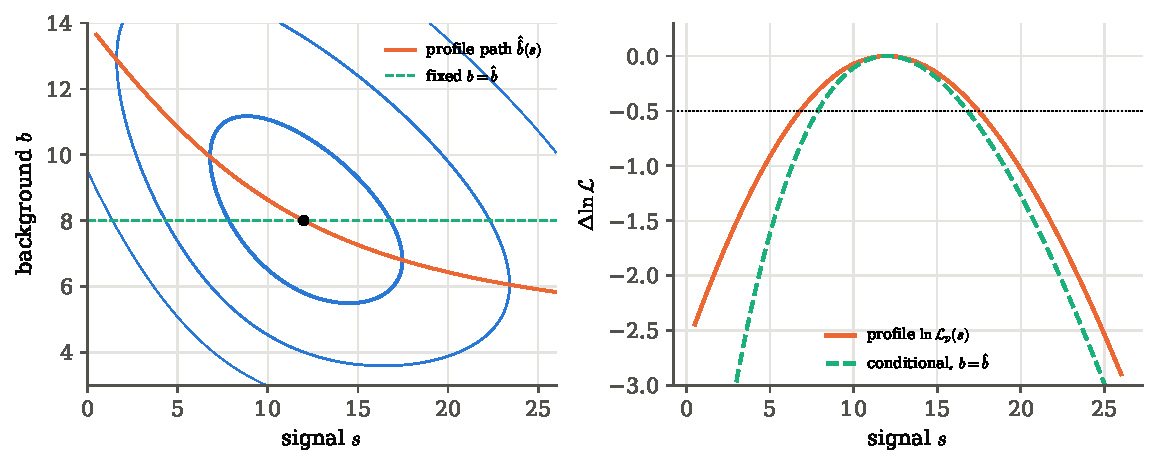
\includegraphics[width=12cm]{figures/ch03/profile.pdf}
\caption{A signal on top of a background, from $20$ counts in the signal
region and $8$ in the control region. Left: contours of $\ln\Like(s,b)$ at
$\Delta\ln\Like=\tfrac12$, $2$ and $4.5$, the profile path (the best
background for each signal value, falling as $s$ rises) and the line of
fixed background. Right: the profile log-likelihood is wider than the
conditional one; the dotted line at $-\tfrac12$ marks the interval
endpoints.}
\label{3b:fig:profile}
\end{figure}

Which interval is right? The script simulates $10^4$ experiments with
$s=12$ and $b=8$ and counts how often each interval contains the true
signal. (In $\ThreeBProfUsed$ of them both intervals exist; the rest have
$n_{\text{off}}=0$ or a similar degenerate outcome.) The profile interval
covers the truth in $\ThreeBProfCover$ of the experiments, the $68\%$ a
$\pm1\sigma$ interval promises. The conditional interval covers it in only
$\ThreeBCondCover$. The reason the profile works is \newterm{Wilks'
theorem} again \cite{Wilks1938}: $-2\ln[\Like_p(\theta)/\Like_{\max}]$ at the
true $\theta$ is asymptotically $\chi^2_1$, whatever the number of nuisance
parameters that were maximised over, so the $\Delta\ln\Like_p=\tfrac12$
interval has $68\%$ coverage for large samples. This is what the
\texttt{MINOS} errors of \texttt{MINUIT} compute, and it is the basis of the
profile-likelihood test statistics used in every LHC search (\cref{ch:04}).

\begin{keyidea}[Profile out nuisance parameters]
Maximise over the nuisance parameters at each value of the parameter of
interest, and read the interval from $\Delta\ln\Like_p=\tfrac12$. For a
Gaussian likelihood this gives exactly the marginal error
$\sqrt{V_{\theta\theta}}$; fixing the nuisance parameters instead gives
$\sqrt{1/F_{\theta\theta}}$, too small by $\sqrt{1-\rho^2}$.
\end{keyidea}

\subsection{Profiling and marginalising}
\label{3b:sec:marginalise}

The Bayesian removes a nuisance parameter differently: by integrating it
out of the posterior, $p(\theta\given\data)=\int p(\theta,\nu\given\data)\,\dd\nu$
\srcref{Padilla}{(38)}, \srcref{HobsonBMC}{p.~49}. This is the
marginalisation of a joint distribution that we have used since
\cref{ch:01}: average over the variable we do not want. For a Gaussian
likelihood and a flat prior the two operations give the same answer,
because the integral of a two-dimensional Gaussian over one variable is a
Gaussian in the other with variance $V_{\theta\theta}$, the same as
\eqref{3b:eq:profile-gauss}. They differ when the likelihood is not
Gaussian, and the difference is itself a warning that the asymptotic
theory is being stretched.

\paragraph{Example: an unknown noise level.}
Hobson et al.\ consider a fit where every datum has Gaussian noise of the
same, unknown size $\sigma$ \srcref{HobsonBMC}{p.~50, (2.25)--(2.26)}. With
$Q(\theta)=\sum_i(D_i-d_i(\theta))^2$ the likelihood is
$\Like(\theta,\sigma)=(2\pi\sigma^2)^{-N/2}\exp[-Q(\theta)/2\sigma^2]$.
Profile over $\sigma$:
\begin{align*}
  \frac{\partial\ell}{\partial\sigma}
  &\eqby{1}-\frac N\sigma+\frac{Q}{\sigma^3}=0
  \ \Rightarrow\ \hat{\hat\sigma}^2(\theta)=\frac{Q(\theta)}{N},
  \qquad
  \Like_p(\theta)\eqby{2}\Bigl(\frac{2\pi Q(\theta)}{N}\Bigr)^{-N/2}e^{-N/2}
  \;\propto\;Q(\theta)^{-N/2} .
\end{align*}
\begin{explain}
  \item Differentiate $-N\ln\sigma-Q/2\sigma^2$.
  \item Substitute: the exponent becomes $-Q/(2Q/N)=-N/2$.
\end{explain}
Now marginalise instead, with the prior $p(\sigma)\propto1/\sigma$ (flat
in $\ln\sigma$, the prior Hobson et al.\ use):
\begin{align*}
  \int_0^\infty\sigma^{-N}e^{-Q/2\sigma^2}\,\frac{\dd\sigma}{\sigma}
  &\eqby{1}\int_0^\infty\Bigl(\frac{2u}{Q}\Bigr)^{N/2}e^{-u}\,\frac{\dd u}{2u}
  \eqby{2}\frac12\Bigl(\frac2Q\Bigr)^{N/2}\Gamma\Bigl(\frac N2\Bigr)
  \;\propto\;Q(\theta)^{-N/2}.
\end{align*}
\begin{explain}
  \item Substitute $u=Q/2\sigma^2$, so $\sigma^{-2}=2u/Q$ and
        $\dd\sigma/\sigma=-\dd u/(2u)$ (the sign is absorbed by swapping the
        limits).
  \item $\int_0^\infty u^{N/2-1}e^{-u}\dd u=\Gamma(N/2)$.
\end{explain}
The two routes give the same function of $\theta$, which is Hobson's
(2.26) up to a constant. The unknown noise level turns the Gaussian
$e^{-\chi^2/2}$ into the heavier-tailed $Q^{-N/2}$, a Student-$t$ shape in
$\theta$ (\cref{ch:02}): not knowing the size of the error bars costs
precision, and the likelihood knows it. The same device, an unknown scale
factor on all quoted error bars, is Hobson's ``safety valve'' for data with
underestimated errors \srcref{HobsonBMC}{p.~52}.
\section{The bootstrap: the sampling distribution from one data set}
\label{3b:sec:bootstrap}

Every error bar so far came from a formula: $\sigma/\sqrt n$ for the mean,
the curvature of $\ln\Like$ for the MLE, the delta method for a function of
estimates. To check those formulas we also used a luxury no experimenter
has: we simulated $10^4$ fresh experiments from the true distribution and
looked at the scatter. Now suppose there is no formula (the median of
lifetimes, a ratio of two fitted amplitudes, the peak position of a
smoothed histogram) and no known truth to simulate from. All we have is one
data set. The \newterm{bootstrap} lets that one data set stand in for the
unknown distribution, and then simulates from it \cite{Efron1979}. Three
questions need answers.
\begin{enumerate}[label=\arabic*.]
  \item What does it mean to ``simulate from the data'', and why does it
        estimate the sampling distribution?
  \item How do we turn the simulated replicas into a standard error and a
        confidence interval?
  \item When does it fail?
\end{enumerate}

\subsection{Two worlds}
\label{3b:sec:boot-idea}

Let the data $x_1,\dots,x_n$ come independently from an unknown
distribution $F$, and let $T_n=g(x_1,\dots,x_n)$ be any statistic. Its
standard error is $\sqrt{\Var_F(T_n)}$, which we could compute by
simulation if we knew $F$: draw many samples of size $n$ from $F$, compute
$T_n$ on each, take the standard deviation. We do not know $F$. But we have
an estimate of it, the \newterm{empirical distribution} $\hat F_n$
\unpack{the distribution that puts probability $1/n$ on each observed data
point, and nothing elsewhere}. The bootstrap replaces $F$ by $\hat F_n$ and
then does the simulation \mainref{pp.~108--109}:
\[
  \Var_F(T_n)\;\overset{\text{(i)}}{\approx}\;\Var_{\hat F_n}(T_n)
  \;\overset{\text{(ii)}}{\approx}\;v_{\text{boot}}
  =\frac1{B-1}\sum_{b=1}^B\Bigl(T^*_{n,b}-\overline{T^*}\Bigr)^2 .
\]
Approximation (i) is the statistical one: it is good when $\hat F_n$ is
close to $F$, which requires $n$ to be reasonably large, and it cannot be
improved without more data. Approximation (ii) is pure Monte Carlo: its
error falls as $1/\sqrt B$, and we make it small by running the computer
longer.

Drawing a sample of size $n$ from $\hat F_n$ means picking $n$ of the
observed points at random, \emph{with replacement}: some points appear
twice or three times, others not at all. Each such \newterm{bootstrap
sample} $x^*_1,\dots,x^*_n$ gives a \newterm{replica} $T^*_n$ of the
statistic. \Cref{3b:fig:two-worlds} lays out the analogy.

\begin{figure}[htbp]
\centering
\begin{tikzpicture}[
  bx/.style={draw=accent,thick,rounded corners=2pt,fill=ideabg,font=\small,
             minimum height=8mm,align=center,text width=25mm},
  bs/.style={bx,draw=fibreorange!80!black,fill=defbg},
  flow/.style={->,thick,accent}]
  \node[bx] (F) at (0,0) {unknown $F$};
  \node[bx] (X) at (3.7,0) {data\\ $x_1,\dots,x_n$};
  \node[bx] (T) at (7.4,0) {$T_n=g(x_1,\dots,x_n)$};
  \draw[flow] (F) -- (X); \draw[flow] (X) -- (T);
  \node[bs] (Fh) at (0,-2.0) {$\hat F_n$: $1/n$ on\\ each data point};
  \node[bs] (Xs) at (3.7,-2.0) {resample\\ $x^*_1,\dots,x^*_n$};
  \node[bs] (Ts) at (7.4,-2.0) {replica\\ $T^*_n=g(x^*_1,\dots,x^*_n)$};
  \draw[flow] (Fh) -- (Xs); \draw[flow] (Xs) -- (Ts);
  \draw[flow,dashed,fibreorange!80!black] (X.south west) to[out=-120,in=60] (Fh.north east);
  \node[font=\small\bfseries,accent,anchor=south west] at (-1.3,0.5) {real world};
  \node[font=\small\bfseries,fibreorange!80!black,anchor=north west] at (-1.3,-2.75) {bootstrap world};
  \node[font=\footnotesize,align=center,anchor=north] at (7.4,-2.75) {repeat $B$ times,\\ histogram the $T^*_n$};
\end{tikzpicture}
\caption{The two worlds of the bootstrap. In the real world an unknown
distribution produced one data set and one value of the statistic, and
we cannot repeat it. In the bootstrap world the empirical distribution
(built from the data, dashed arrow) plays the role of the truth. We can
draw from it as often as we like, and the scatter of the replicas stands in
for the scatter of the statistic in the real world.}
\label{3b:fig:two-worlds}
\end{figure}

\begin{workdef}[nonparametric bootstrap]
To estimate the standard error of a statistic $T_n$ from one data set of
size $n$: for $b=1,\dots,B$, draw $n$ indices uniformly from
$\{1,\dots,n\}$ with replacement, form the bootstrap sample, and compute the
replica $T^*_{n,b}$. The bootstrap standard error is the sample standard
deviation of the $B$ replicas \mainref{p.~109, (8.1)}. $B$ of a few hundred
suffices for a standard error; intervals need a few thousand.
\end{workdef}

\paragraph{Example: the bootstrap of the mean, exactly.}
For the mean we can do the bootstrap world by hand. A single resampled
point $x^*$ equals each $x_i$ with probability $1/n$, so
\begin{align*}
  \E_{\hat F}x^*&\eqby{1}\frac1n\sum_ix_i=\bar x,\qquad
  \Var_{\hat F}x^*\eqby{2}\frac1n\sum_i(x_i-\bar x)^2\equiv\hat\sigma^2,\\
  \Var_{\hat F}\bar x^*&\eqby{3}\frac{\hat\sigma^2}{n}
  \eqby{4}\frac{n-1}{n}\,\frac{S^2}{n} .
\end{align*}
\begin{explain}
  \item The expectation over the empirical distribution is the plain
        average of the data.
  \item Its variance is the average squared deviation from that average,
        with divisor $n$.
  \item The $n$ resampled points are independent draws from $\hat F$, so the
        variance of their mean is the single-point variance over $n$.
  \item $S^2=\sum_i(x_i-\bar x)^2/(n-1)$ is the unbiased sample variance.
\end{explain}
The bootstrap reproduces the textbook standard error $S/\sqrt n$, up to the
factor $\sqrt{(n-1)/n}$ that is negligible for $n$ of a few tens. For the
data $\{1,2,6\}$, $\bar x=3$ and $\hat\sigma^2=(4+1+9)/3=14/3$, so the
bootstrap variance of the mean is $14/9=1.56$, against $S^2/n=7/3=2.33$ from
the unbiased formula: with three points the factor $(n-1)/n=2/3$ matters.
There are only $\binom{2n-1}{n}=10$ distinct bootstrap samples here, so for
tiny $n$ the bootstrap distribution is coarse; for $n=50$ there are about
$5\times10^{28}$.

\paragraph{The parametric bootstrap.}
If we trust a parametric model $f(x;\theta)$, there is a better stand-in
for $F$ than $\hat F_n$: the fitted model $f(x;\hat\theta)$. The
\newterm{parametric bootstrap} simulates $B$ data sets of size $n$ from
$f(x;\hat\theta)$ and refits each one \mainref{p.~134}. This is exactly
what we did with the $10^4$ simulated lifetime experiments of
\cref{3b:sec:curv-python}, except that the fitted value replaces the truth.
It is also the standard way to calibrate a
complicated analysis in physics: fit, simulate from the fit, analyse the
simulations the same way, look at the scatter.

\subsection{The bootstrap in Python}
\label{3b:sec:boot-python}

The script \pyname{15_bootstrap.py} takes one data set of $n=50$ decay
times and asks for the standard errors of two statistics: the mean
$\hat\tau$, where we know the answer, and the median, where we have no
simple formula (its asymptotic variance is $1/[4nf(m)^2]$ from
\cref{3b:sec:efficiency}, which needs the unknown density at the unknown
median).
\pyfile[firstline=26,lastline=45]{code/ch03/15_bootstrap.py}{Nonparametric and parametric bootstrap of the mean and the median}
Line 34 is the whole nonparametric bootstrap: a $B\times n$ array of random
indices, used to pick data points with replacement, so that each row is one
bootstrap sample. Line 38 is the parametric bootstrap, fresh exponential
samples with the fitted lifetime. Lines 30--31 compute what no experimenter
can, the true sampling distribution from $10^4$ fresh experiments, as a
referee.

\begin{center}
\small
\begin{tabular}{lccc}
  \hline
  standard error & true (fresh experiments) & nonparametric & parametric\\
  \hline
  mean $\hat\tau$ & $\ThreeBBootSeTauTrue$ & $\ThreeBBootSeTauNP$ & $\ThreeBBootSeTauP$\\
  median & $\ThreeBBootSeMedTrue$ & $\ThreeBBootSeMedNP$ & $\ThreeBBootSeMedP$\\
  \hline
\end{tabular}
\end{center}
In this run the data set has $\hat\tau=\ThreeBBootTauHat$ and median
$\ThreeBBootMed$, for true values $1$ and $\ln2=\ThreeBBootMedTrueVal$.
The bootstrap estimates the standard error of the distribution it simulates
from, and that distribution is built from these fifty numbers, so it
inherits their luck. The parametric bootstrap simulates from an exponential
with mean $\hat\tau$, so its error for the mean follows $\hat\tau$, as does
the curvature error $\hat\tau/\sqrt n=\ThreeBBootSeTauCurv$. The
nonparametric bootstrap follows the spread of the data instead. A data set
that comes out low or narrow gives error bars that are too small, one that
comes out high or wide gives error bars that are too large, and no method
that uses only these fifty numbers can tell which kind of draw it has.
Dividing by the estimate removes the overall scale: the \emph{relative}
error here is $\ThreeBBootSeTauNP/\ThreeBBootTauHat=\ThreeBBootRelOne$
against the true $\ThreeBBootSeTauTrue/1$. That too depends on the draw.
Computed on each of the $10^4$ fresh experiments, the same relative error
averages $\ThreeBBootRelMean$ but scatters by $\ThreeBBootRelSd$ from one
data set to the next, so a single data set can easily miss it by that much.
For the median the bootstrap gives an error bar where we had no formula at
all, with the same caveat: it comes from one data set and shares its luck. \Cref{3b:fig:bootstrap} compares the shapes of the bootstrap
distributions, each centred on its own estimate, with the true sampling
distribution.

\begin{figure}[htbp]
\centering
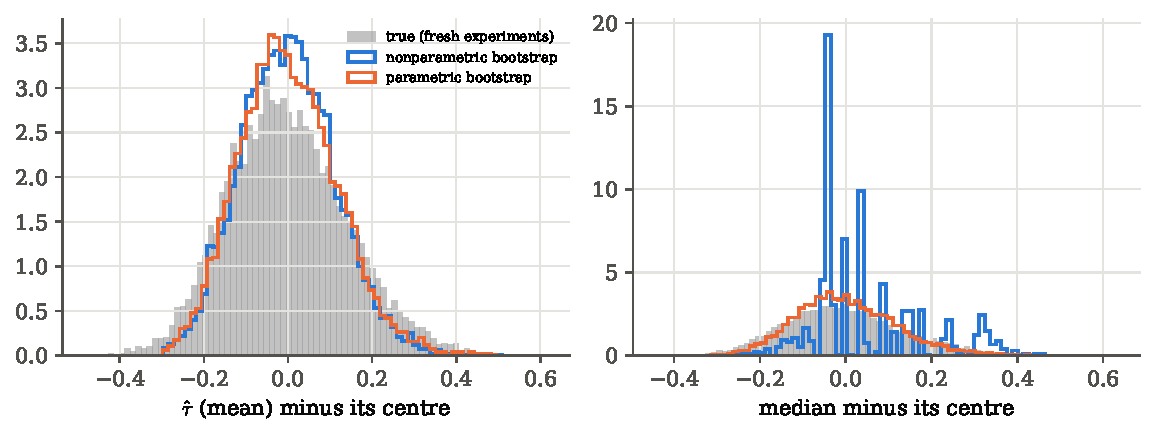
\includegraphics[width=12cm]{figures/ch03/bootstrap.pdf}
\caption{Bootstrap distributions from one data set of fifty decay times,
each centred on its own centre so the shapes can be compared. Grey: the true
sampling distribution from ten thousand fresh experiments. Blue: resampling
the data with replacement. Orange: simulating from the fitted exponential.
Left: the mean. Right: the median, whose nonparametric bootstrap
distribution is lumpy because a resampled median can only take a few
values near the middle of the data.}
\label{3b:fig:bootstrap}
\end{figure}

\subsection{Bootstrap confidence intervals}
\label{3b:sec:boot-intervals}

A standard error gives the simplest interval, the \newterm{Normal
interval} $T_n\pm z_{\alpha/2}\,\widehat{\mathrm{se}}_{\text{boot}}$
\mainref{p.~110, (8.2)}, which assumes a Gaussian sampling distribution. The
bootstrap distribution contains more than a width, and two other
constructions use its shape.

\paragraph{The pivotal interval.}
Let $R_n=\hat\theta-\theta$ be the error of the estimate, with unknown
distribution function $H(r)=\Prob(R_n\le r)$. Choose
$a=\hat\theta-H^{-1}(1-\alpha/2)$ and $b=\hat\theta-H^{-1}(\alpha/2)$. Then
\begin{align*}
  \Prob(a\le\theta\le b)
  &\eqby{1}\Prob\bigl(\hat\theta-b\le R_n\le\hat\theta-a\bigr)
  \eqby{2}H\bigl(\hat\theta-a\bigr)-H\bigl(\hat\theta-b\bigr)\\
  &\eqby{3}H\bigl(H^{-1}(1-\tfrac\alpha2)\bigr)-H\bigl(H^{-1}(\tfrac\alpha2)\bigr)
  =1-\alpha .
\end{align*}
\begin{explain}
  \item $a\le\theta$ is the same as $\hat\theta-\theta\le\hat\theta-a$, and
        $\theta\le b$ is $\hat\theta-b\le\hat\theta-\theta$.
  \item Probability of an interval from the distribution function (for a
        continuous $H$).
  \item Insert the chosen $a$ and $b$.
\end{explain}
We do not know $H$, but the bootstrap gives its analogue: the distribution
of $R^*=\theta^*-\hat\theta$, whose quantiles are
$\theta^*_\beta-\hat\theta$ with $\theta^*_\beta$ the $\beta$-quantile of
the replicas. Substituting gives the \newterm{pivotal interval}
\mainref{p.~111, (8.6)}
\[
  C_n=\bigl(2\hat\theta-\theta^*_{1-\alpha/2},\ 2\hat\theta-\theta^*_{\alpha/2}\bigr).
\]
The interval is reflected. Suppose the replicas scatter further above
$\hat\theta$ than below it. In the bootstrap world, then, the estimate
overshoots its truth by larger amounts than it undershoots. Carried back to
the real world, our $\hat\theta$ may sit well above the true $\theta$, so
the interval reaches further \emph{down}.

\paragraph{The percentile interval.}
The simplest recipe of all takes the quantiles of the replicas directly,
$(\theta^*_{\alpha/2},\theta^*_{1-\alpha/2})$ \mainref{p.~111}. It is exact
when some monotone transformation makes the sampling distribution symmetric
and Gaussian, and it respects the parametrisation in the way the
$\Delta\ln\Like$ interval does. All three intervals have coverage tending to
$1-\alpha$ under weak conditions \mainref{p.~111, Thm.~8.3}.

\paragraph{Example: the median of the lifetimes.}
For the median of our fifty decay times, $95\%$ intervals from $10^4$
nonparametric replicas are
\[
  \text{Normal: }(\ThreeBBootNormLo,\ \ThreeBBootNormHi),\qquad
  \text{pivotal: }(\ThreeBBootPivLo,\ \ThreeBBootPivHi),\qquad
  \text{percentile: }(\ThreeBBootPctLo,\ \ThreeBBootPctHi),
\]
for a true median of $\ThreeBBootMedTrueVal$. The replicas of a median are
lumpy and lopsided, and the three recipes treat the lopsidedness
differently: the percentile interval follows it, the pivotal interval
reflects it about the estimate, and the Normal interval ignores it. So the
three intervals differ, and for one data set one of them can miss the true
median while another contains it. Any $95\%$ procedure
misses in one experiment in twenty. Which of them misses less often for a
given problem can be settled only by the same kind of simulation over many
data sets, as in \cref{ch:04}.

\subsection{Where the bootstrap fails}
\label{3b:sec:boot-fail}

The bootstrap works when the statistic depends smoothly on the whole
distribution. It fails when the statistic is controlled by a few extreme
points, because $\hat F_n$ has no probability beyond the largest observation.
The cleanest example is the uniform box again, with $T_n=x_{(n)}$. The true
sampling distribution of the maximum is continuous, with density
$nx^{n-1}/\theta^n$ below $\theta$. A bootstrap replica, however, is the
maximum of $n$ points drawn from the data, and it equals the observed
maximum whenever that point is drawn at least once:
\begin{align*}
  \Prob\bigl(x^*_{(n)}=x_{(n)}\bigr)
  &\eqby{1}1-\Prob\bigl(x_{(n)}\text{ is never drawn}\bigr)
  \eqby{2}1-\Bigl(1-\frac1n\Bigr)^n
  \;\xrightarrow{n\to\infty}\;1-e^{-1}=0.632 .
\end{align*}
\begin{explain}
  \item The replica's maximum is $x_{(n)}$ as soon as $x_{(n)}$ is among the
        resampled points; otherwise it is smaller.
  \item Each of the $n$ independent draws misses that point with probability
        $1-1/n$.
\end{explain}
For $n=50$ this is $\ThreeBBootFracTh$, and the simulation gives
$\ThreeBBootFrac$: almost two thirds of the replicas sit on a single value,
a spike that the continuous true distribution does not have
(\cref{3b:fig:bootstrap-fail}). No amount of resampling can put a replica
above $x_{(n)}$, yet the true $\theta$ is always there. The same caution
applies to any statistic that lives in the tails: extreme values, endpoint
fits, the largest peak in a noisy map. For such statistics the parametric
bootstrap, or a simulation from a physical model, is the right tool.

\begin{figure}[htbp]
\centering
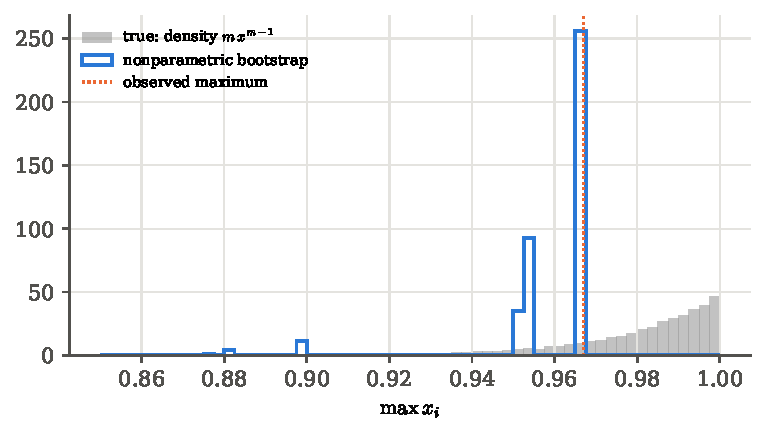
\includegraphics[width=9cm]{figures/ch03/bootstrap_uniform.pdf}
\caption{A statistic the bootstrap cannot handle: the maximum of fifty
uniform points. Grey: its true sampling distribution, smooth and piled
against the end of the box. Blue: the bootstrap replicas, about
$63\%$ of which equal the observed maximum (dotted line), with the rest
spread over a few lower data values. None can exceed the observed maximum.}
\label{3b:fig:bootstrap-fail}
\end{figure}

\begin{inpractice}[Verification versus research]
Most of the simulations above \emph{verified} results already derived:
that $\chi^2_{\min}$ follows $\chi^2_{N-m}$, that the curvature
of $\ln\Like$ equals the scatter of the MLE, that the Poisson fit conserves
the total. Their job was to make the formulas believable and to show how
large $n$ must be before the asymptotic statements hold. In research the
same machinery is the instrument itself, used exactly where no formula
exists. A cosmological analysis estimates the covariance matrix of a
masked, noisy power spectrum from hundreds of simulated skies, a
parametric bootstrap from the fitted model (\cref{ch:07,ch:08}); an LHC
search calibrates its profile-likelihood test statistic on pseudo-experiments
when Wilks' theorem is doubtful; large-scale-structure analyses resample
patches of the sky (a jackknife or block bootstrap) to capture
correlations no one can model analytically. The logic is always that of
\cref{3b:fig:two-worlds}: build the best stand-in for the truth, simulate
from it, analyse each simulation exactly as the data, read the error off the
scatter.
\end{inpractice}
\section{From a model to an estimator: how to find the right one}
\label{3b:sec:recipe}

A theorist hands us a model: a prediction $d(\theta)$, a noise level, and a
parameter $\theta$ to be measured. Nothing says which function of the data
to quote as the answer. The sample mean, the median, the midrange, the
value that minimises some $\chi^2$: each is an estimator, each has a
sampling distribution, and they differ in width. So the question is: which
function of the data should we quote? The tools for answering it are
already in hand. The likelihood gives the probability of the data. The
score equation turns it into an estimate. The curvature gives an error bar.
The Cram\'er--Rao bound says how narrow the error bar can ever be. Put in
order, these tools become a procedure that starts from the model and ends
with an estimator whose sampling distribution we know and cannot improve
(\cref{3b:fig:recipe-flow}). The procedure has five steps, and every one has
already appeared in a special case.

\begin{figure}[htbp]
\centering
\begin{tikzpicture}[
  bx/.style={draw=accent,thick,rounded corners=2pt,fill=ideabg,font=\small,
             minimum height=9mm,align=center,text width=33mm},
  bd/.style={bx,dashed,draw=fibreorange!80!black,fill=defbg},
  flow/.style={->,thick,accent}]
  \node[bx] (A) at (0,0)   {1. model\\ $\data=d(\theta)+\text{noise}$};
  \node[bx] (B) at (4.4,0) {likelihood\\ $\Like(\theta)=p(\data\given\theta)$};
  \node[bx] (C) at (8.8,0) {2. sufficient\\ statistic $U(\data)$};
  \node[bx] (D) at (8.8,-3.3) {3. candidates: moments, ML, LS, Bayes};
  \node[bx] (E) at (4.4,-3.3) {4. best? bias, variance, Cram\'er--Rao, Rao--Blackwell};
  \node[bx] (F) at (0,-3.3) {estimate $\hat\theta\pm\hat\sigma$};
  \node[bd] (G) at (4.4,-1.65) {5. no formula:\\ simulate and calibrate};
  \draw[flow] (A) -- (B); \draw[flow] (B) -- (C); \draw[flow] (C) -- (D);
  \draw[flow] (D) -- (E); \draw[flow] (E) -- (F);
  \draw[flow,dashed,fibreorange!80!black] (B) -- (G);
  \draw[flow,dashed,fibreorange!80!black] (G) -- (E);
\end{tikzpicture}
\caption{From a model to an estimator. The solid path is the procedure when
the likelihood can be written down. If it cannot (dashed path), a simple
statistic is computed and its bias and scatter are read off simulated
data sets.}
\label{3b:fig:recipe-flow}
\end{figure}

Four examples run through every step: independent Gaussian readings
$x_i\sim\Normal(\mu,\sigma^2)$ with known $\sigma$; Poisson counts
$X_i\sim\mathrm{Poisson}(\lambda)$, the numbers of events in $n$ equal time
slots; exponential decay times $t_i$ with mean lifetime $\tau$; and the
multipole coefficients $\alm$ of a full-sky Gaussian CMB map. The CMB
example is then followed through the whole chain in
\cref{3b:sec:recipe-cmb}.

\subsection{Step 1: write the likelihood}
\label{3b:sec:recipe-like}

Everything starts from the statement that the data are the model plus noise
(\cref{3b:sec:one-measurement}): the noise realisation that the data require
has a known probability, and that probability, read as a function of the
parameter, is $\Like(\theta)$. For independent data the likelihood is the
product \eqref{3b:eq:like-iid}. For the four examples, keeping only the
factors that depend on the parameter,
\begin{align}
  \text{Gaussian mean:}\quad &\Like(\mu)\propto
      \exp\Bigl[-\frac1{2\sigma^2}\sum_i(x_i-\mu)^2\Bigr],
  \nonumber\\
  \text{Poisson rate:}\quad &\Like(\lambda)=\prod_i\frac{e^{-\lambda}\lambda^{X_i}}{X_i!}
      \propto e^{-n\lambda}\lambda^{K},\qquad K\equiv\sum_iX_i,
  \nonumber\\
  \text{exponential lifetime:}\quad &\Like(\tau)=\tau^{-n}e^{-T/\tau},\qquad
      T\equiv\sum_it_i,
  \label{3b:eq:four-likes}\\
  \text{full-sky CMB:}\quad &\Like(\Cell)\propto
      \Cell^{-(2\ell+1)/2}\exp\Bigl[-\frac{(2\ell+1)\Chat}{2\Cell}\Bigr].
  \nonumber
\end{align}
The last line is the isotropic Gaussian sky of \cref{3b:sec:universal}.
Recall its ingredients. At multipole $\ell$ there are $2\ell+1$ independent
real numbers $y_{\ell k}$: $a_{\ell0}$, and $\sqrt2\,\mathrm{Re}\,\alm$ and
$\sqrt2\,\mathrm{Im}\,\alm$ for $m=1,\dots,\ell$. (For $m>0$ the real and
imaginary parts of $\alm$ each have variance $\Cell/2$, and $a_{\ell,-m}$ is
the complex conjugate of $\alm$ up to a sign, so it adds nothing new; the
factor $\sqrt2$ brings each variance up to $\Cell$.) Each $y_{\ell k}$ has
density $(2\pi\Cell)^{-1/2}e^{-y_{\ell k}^2/2\Cell}$. Their product over the
$2\ell+1$ values of $k$ gives the last line, with
$(2\ell+1)\Chat=\sum_ky_{\ell k}^2=\sum_m|\alm|^2$.

\subsection{Step 2: what can the data tell us? Sufficient statistics}
\label{3b:sec:recipe-suff}

Look at \eqref{3b:eq:four-likes}. The Gaussian likelihood contains the
$n$ readings, yet after expanding the square it depends on them only through
$\bar x$ (and through a constant). The Poisson likelihood depends on the
counts only through their total $K$, the exponential one only through $T$,
the CMB one only through $\Chat$. Every data set with the same $K$ gives
exactly the same likelihood curve, so no estimate, error bar or confidence
interval computed from the likelihood can distinguish them. The remaining
information in the $n$ numbers, which ones were large, which came first,
says nothing about $\theta$.

\paragraph{Definition.}
A statistic $U(\data)$ is \newterm{sufficient} for $\theta$ if the
conditional distribution of the data given the value of $U$ does not involve
$\theta$ \mainref{p.~137, Def.~9.32}. Given $U$, the data set is one of the
points on the ``surface'' $\{\data':U(\data')=U(\data)\}$, and sufficiency
says that $\theta$ has no influence on which point of the surface we land
on: $\theta$ only decides how probable the surface is. Statistical
mechanics has met this before. In the canonical ensemble
$p(\text{microstate}\given\beta)=e^{-\beta E}/Z(\beta)$, and given the energy
$E$ all microstates are equally likely, whatever $\beta$ is. The energy is
therefore a sufficient statistic for the inverse temperature $\beta$: a
thermometer that reads only $E$ loses nothing.

The coarsest statistic with this property is called \newterm{minimal
sufficient}: two data sets have the same value of it exactly when the ratio
of their likelihoods $p(\data\given\theta)/p(\data'\given\theta)$ does not
depend on $\theta$ \mainref{p.~138, Def.~9.35}. In all the examples below the statistic
found is minimal, so no further compression is possible without losing
information.

\paragraph{The factorisation theorem.}
Checking the definition directly needs the conditional distribution. The
\newterm{Neyman--Fisher factorisation theorem} \mainref{p.~140, Thm.~9.40},
\srcref{CasellaBerger}{Thm.~6.2.6} replaces that with a test on the
likelihood:
\[
  U\text{ is sufficient}\iff
  p(\data\given\theta)=g\bigl(U(\data),\theta\bigr)\,h(\data)
  \quad\text{for some functions }g,h .
\]
All the $\theta$-dependence must pass through $U$, and whatever else depends
on the data (the $h$) must not know about $\theta$. The proof, for discrete
data (sums become integrals for densities), has two halves. Write $\mathcal A_u$ for
the set of all data sets with $U=u$.

\emph{Factorised form implies sufficiency.} For a data set $\data$ with
$U(\data)=u$,
\begin{align}
  \Prob(\data\given U=u,\theta)
  &\eqby{1}\frac{\Prob(\data\given\theta)}{\Prob(U=u\given\theta)}
   \eqby{2}\frac{g(u,\theta)\,h(\data)}{\sum_{\data'\in\mathcal A_u}g(u,\theta)\,h(\data')}
   \eqby{3}\frac{h(\data)}{\sum_{\data'\in\mathcal A_u}h(\data')} .
  \label{3b:eq:suff-forward}
\end{align}
\begin{explain}
  \item The event $\{\data\}$ lies inside $\{U=u\}$, so
        $\Prob(\data,U=u\given\theta)=\Prob(\data\given\theta)$.
  \item Numerator by the factorisation. The denominator is the sum of the
        probabilities of all data sets in $A_u$, and $g(U(\data'),\theta)=g(u,\theta)$
        for each of them.
  \item $g(u,\theta)$ is a common factor and cancels.
\end{explain}
The result contains no $\theta$, which is the definition.

\emph{Sufficiency implies the factorised form.} If
$\Prob(\data\given U=u,\theta)=c(\data)$ does not depend on $\theta$, then
\[
  \Prob(\data\given\theta)
  =\Prob(\data\given U=U(\data),\theta)\,\Prob(U=U(\data)\given\theta)
  =c(\data)\;q\bigl(U(\data),\theta\bigr),
\]
which is the factorised form with $h=c$ and $g=q$, the sampling distribution
of $U$ itself.

\paragraph{Examples.}
Expanding the square, $\sum_i(x_i-\mu)^2=\sum_i(x_i-\bar x)^2+n(\bar x-\mu)^2$,
so the Gaussian likelihood factorises with
$g=\exp[-n(\bar x-\mu)^2/2\sigma^2]$ and $h=\exp[-\sum_i(x_i-\bar x)^2/2\sigma^2]$:
$\bar x$ is sufficient for $\mu$. Reading \eqref{3b:eq:four-likes}, the Poisson
total $K$ is sufficient for $\lambda$ with $g=e^{-n\lambda}\lambda^K$ and
$h=\prod_i1/X_i!$; the sum of decay times $T$ is sufficient for $\tau$ with
$h=1$; and $\Chat$, equivalently $\sum_m|\alm|^2$, is sufficient for $\Cell$
with $h=1$. The last statement is the precise form of the everyday remark
that for a Gaussian isotropic sky the power spectrum contains everything
there is to know about the parameters: the phases of the $\alm$ carry no
information. It is a statement about the model. If the field is not
Gaussian, $h$ is no longer free of $\Cell$ and the phases carry information
that $\Chat$ throws away, a point that returns when topological summaries of
fields appear (\cref{ch:12}).

\paragraph{The exponential family: sufficient statistics and moment matching.}
All four examples, and most of the distributions of \cref{ch:02},
have the form
\begin{equation}
  p(x\given\theta)=h(x)\exp\bigl[\eta(\theta)\,\phi(x)-A(\theta)\bigr],
  \label{3b:eq:expfam}
\end{equation}
with $\phi(x)$ a single function of one observation (the Poisson has
$\phi=x$, $\eta=\ln\lambda$, $A=\lambda$; the exponential lifetime has
$\phi=t$, $\eta=-1/\theta$, $A=\ln\theta$ with $\theta$ the mean lifetime; the CMB coefficient has
$\phi=y^2$, $\eta=-1/2\Cell$, $A=\tfrac12\ln2\pi\Cell$). For $n$
independent observations, the product has
$\exp[\eta\sum_i\phi(x_i)-nA]\prod_ih(x_i)$, so $\sum_i\phi(x_i)$ is
sufficient by the factorisation theorem. More: the MLE is the solution of
a moment-matching equation. Differentiating the normalisation
$\int p\,\dd x=1$ with respect to $\theta$ gives
\[
  0=\int(\eta'\phi-A')\,p\,\dd x
  \quad\Longrightarrow\quad
  \E_\theta\phi=\frac{A'(\theta)}{\eta'(\theta)},
\]
and then
\begin{align}
  \frac{\partial\ell}{\partial\theta}
  &\eqby{1}\eta'\sum_i\phi(x_i)-nA'
   \eqby{2}\eta'(\theta)\Bigl[\sum_i\phi(x_i)-n\,\E_\theta\phi\Bigr] .
  \label{3b:eq:expfam-score}
\end{align}
\begin{explain}
  \item Logarithm of the product, then differentiate; $h$ does not contain $\theta$.
  \item Insert $A'=\eta'\,\E_\theta\phi$.
\end{explain}
With $\eta'\ne0$ the score equation is
\begin{equation}
  \E_{\hat\theta}\,\phi=\frac1n\sum_{i=1}^n\phi(x_i),
  \label{3b:eq:moment-match}
\end{equation}
\emph{the model's mean of the sufficient statistic equals its observed
mean.} That is why the maximum-likelihood lifetime is the mean decay time,
the Poisson rate estimate is the mean count $\hat\lambda=\bar X$, the CMB
estimate is the mean of $y^2$, and in each case the method of moments
(\cref{3b:sec:mom}) gives the same answer as maximum likelihood. Outside the
exponential family, for instance for the angular distribution
\eqref{3b:eq:angular}, whose parameters also sit in the normalisation, the two
methods give different estimates and the moment estimates are generally less precise.

\subsection{Step 3: constructing candidate estimators}
\label{3b:sec:recipe-candidates}

Having found what the data can tell us, we build estimators from it. The
families met so far are the following.
\begin{itemize}
  \item \emph{Method of moments} (\cref{3b:sec:mom}): set model moments equal
        to sample moments. No likelihood is needed, only moments of the
        model. Quick, consistent, often a good starting point for Newton--Raphson.
  \item \emph{Maximum likelihood} (\cref{3b:sec:mle}): maximise
        $\Like(\theta)$. Always available when the likelihood is, invariant
        under reparametrisation, asymptotically efficient.
  \item \emph{Least squares} (\cref{3b:sec:ls-from-ml}): the maximum likelihood estimator
        for independent Gaussian noise, $-2\ell=\chi^2$, and for correlated
        Gaussian noise with the weight matrix $\Cmat^{-1}$. Not a separate
        principle.
  \item \emph{Bayes estimators}, which use a prior and a cost of being wrong.
        They complete the list and are derived below; \cref{ch:05}
        develops them.
\end{itemize}

\paragraph{The EM algorithm: maximum likelihood with hidden variables.}
Sometimes the likelihood is a sum over quantities we did not observe, such as the
unknown class of each event in a mixture of signal and background,
$p(\data\given\theta)=\sum_zp(\data,z\given\theta)$, and the logarithm of a sum
has no closed-form maximum. Given a current guess $\theta_t$, let
$q(z)=p(z\given\data,\theta_t)$ be the posterior probability of each hidden
assignment. Since the logarithm is concave, Jensen's inequality gives
\begin{align}
  \ln p(\data\given\theta)
  &\eqby{1}\ln\sum_zq(z)\frac{p(\data,z\given\theta)}{q(z)}
   \relby{2}{\ge}\sum_zq(z)\ln p(\data,z\given\theta)-\sum_zq(z)\ln q(z),
  \label{3b:eq:em}
\end{align}
\begin{explain}
  \item Multiply and divide by $q(z)$, which sums to one.
  \item Jensen: the log of an average is at least the average of the log.
\end{explain}
with equality at $\theta=\theta_t$. (There
$p(\data,z\given\theta_t)/q(z)=p(\data\given\theta_t)$ is the same for every
$z$, and Jensen's inequality is an equality for an average of equal
numbers.) The right side differs from
$Q(\theta\given\theta_t)=\sum_zq(z)\ln p(\data,z\given\theta)$ by a constant,
and $Q$ involves the logarithm of a single term, usually easy to maximise.
The algorithm alternates the \newterm{E step} (compute $q(z)$, hence $Q$) with
the \newterm{M step} ($\theta_{t+1}=\arg\max_\theta Q$). No cycle can
decrease the likelihood, because the right side touches $\ln p(\data\given\theta)$ at
$\theta_t$ and lies below it elsewhere \mainref{pp.~143--144}. Raising the
right side therefore raises $\ln p$ at least as much. It converges to a
stationary point, which can be a local maximum.

\paragraph{Bayes estimators: choose the answer that minimises the expected loss.}
Suppose we must announce one number $a$ for $\theta$, and being off by
$\theta-a$ costs us $L(\theta,a)$. We do not know $\theta$, but after the
experiment we have the posterior $p(\theta\given\data)\propto
\Like(\theta)p(\theta)$, the probability density of the value of $\theta$ given the
data and a prior $p(\theta)$ (\cref{3b:eq:bayes}). Announce the $a$ that
minimises the posterior expected loss
\[
  \rho(a)=\int L(\theta,a)\,p(\theta\given\data)\,\dd\theta .
\]
The expectation is over the plausible values of $\theta$ at fixed data,
not over repeated data sets. Three choices of loss give three familiar
summaries.

\emph{Squared loss, $L=(\theta-a)^2$.} Let $m=\E[\theta\given\data]$ be the
posterior mean. Then
\begin{align}
  \rho(a)&=\E\bigl[(\theta-a)^2\given\data\bigr]\\
   &\eqby{1}\E\bigl[(\theta-m)^2\given\data\bigr]
     +2(m-a)\,\E\bigl[\theta-m\given\data\bigr]+(m-a)^2\\
   &\eqby{2}\Var[\theta\given\data]+(m-a)^2 .
  \label{3b:eq:bayes-squared}
\end{align}
\begin{explain}
  \item Write $\theta-a=(\theta-m)+(m-a)$ and expand the square. The number
        $m-a$ is a constant for the expectation.
  \item $\E[\theta-m\given\data]=0$ by definition of $m$, which kills the cross term.
\end{explain}
The first term does not depend on $a$, so $\rho$ is smallest at $a=m$: the
\emph{posterior mean} minimises the expected squared error.

\emph{Absolute loss, $L=|\theta-a|$.} With $F(a)=\int_{-\infty}^ap\,\dd\theta$,
\begin{align*}
  \rho(a)&=\int_{-\infty}^{a}(a-\theta)\,p\,\dd\theta+\int_a^\infty(\theta-a)\,p\,\dd\theta,\\
  \frac{\dd\rho}{\dd a}&\eqby{1}\int_{-\infty}^{a}p\,\dd\theta-\int_a^\infty p\,\dd\theta
   =2F(a)-1 .
\end{align*}
\begin{explain}
  \item Differentiate the integrals with respect to $a$ in the integrand and
        at the limits; the limit terms contain $(a-\theta)p$ at $\theta=a$, which is zero.
\end{explain}
The derivative vanishes at $F(a)=\tfrac12$: the \emph{posterior median}.

\emph{Zero--one loss,} $L=0$ if $|\theta-a|<h$ and $1$ otherwise. Then
$\rho(a)=1-\int_{a-h}^{a+h}p\,\dd\theta\approx1-2h\,p(a\given\data)$, smallest
where the posterior is largest: the \emph{posterior mode} (MAP, maximum
\emph{a posteriori}), obtained as $h\to0$.

For a symmetric, single-peaked posterior the three coincide. For a skewed
one they do not. The Poisson rate with a single observation $K=2$ and a flat
prior has posterior $p(\lambda\given K)\propto\lambda^2e^{-\lambda}$, a
Gamma density with shape $3$. Its mode is $2$ (equal to the MLE, because the
prior is flat, \cref{3b:sec:bayes-place}), its median is $2.67$ and its
mean is $3$. Evaluating the expected losses on a grid of announced values
(\cref{3b:fig:recipe}, middle) reproduces the three minima at
$\ThreeBBayesZOArg$, $\ThreeBBayesAbsArg$ and $\ThreeBBayesSqArg$. Which
number is ``the estimate'' depends on what a mistake costs. A flat prior
makes the maximum-likelihood estimate the Bayes estimator under zero--one
loss, and only under it.

\subsection{Step 4: choosing the best}
\label{3b:sec:recipe-best}

Several candidates, several sampling distributions. Two tools rank them.
The first is the Cram\'er--Rao bound (\cref{3b:sec:cramer-rao}), a floor on
the variance of an unbiased estimator. If a candidate sits on the floor it
cannot be improved, and the search ends. The second tool says how to
improve a candidate that is above it.

\paragraph{The Rao--Blackwell theorem.}
Let $W(\data)$ be any unbiased estimator of $g(\theta)$ and $U$ a sufficient
statistic. Define
\[
  \tilde W(U)=\E[W\given U] ,
\]
the average of $W$ over all data sets with the observed value of $U$.
Three facts follow.

First, $\tilde W$ is a legitimate statistic. The average uses the
conditional distribution of the data given $U$, which by sufficiency does not
contain $\theta$. Without sufficiency the average would need the unknown
$\theta$ and could not be computed.

Second, $\tilde W$ is unbiased, by the law of total expectation,
$\E\tilde W=\E[\E(W\given U)]=\E W=g(\theta)$.

Third, its variance is never larger:
\begin{align}
  \Var W
  &\eqby{1}\E\bigl[\Var(W\given U)\bigr]+\Var\bigl[\E(W\given U)\bigr]
   \eqby{2}\E\bigl[\Var(W\given U)\bigr]+\Var\tilde W
   \relby{3}{\ge}\Var\tilde W .
  \label{3b:eq:rao-blackwell}
\end{align}
\begin{explain}
  \item The law of total variance: split the scatter of $W$ into the average
        scatter inside each slice $U=u$ and the scatter of the slice
        averages between slices.
  \item Definition of $\tilde W$.
  \item The first term is an average of variances, each $\ge0$. It vanishes
        only if $W$ is already a function of $U$.
\end{explain}
\mainref{p.~140, Thm.~9.42}, \srcref{CasellaBerger}{Thm.~7.3.17}. The
reduction is exactly the average variance that $W$ wasted on the part of the
data that $U$ does not contain. The theorem gives an algorithm: start with
any crude unbiased estimator, however silly, and average it over the
sufficient statistic.

\paragraph{Example: estimating $e^{-\lambda}$, the chance of an empty slot.}
In $n$ time slots we count $X_i\sim\mathrm{Poisson}(\lambda)$ events, and we
want $g(\lambda)=e^{-\lambda}=\Prob(X=0)$, the probability that a slot is
empty. A crude unbiased estimator uses the first slot only:
$W=\mathbf 1\{X_1=0\}$, since $\E W=\Prob(X_1=0)=e^{-\lambda}$. It wastes
$n-1$ slots. Its variance is that of a 0/1 variable, $e^{-\lambda}(1-e^{-\lambda})$.
The total $K=\sum_iX_i$ is sufficient. The conditional mean is the
probability that slot $1$ is empty given the total $K=s$. Independent
Poisson variables add to a Poisson variable, so
\begin{align}
  \Prob(X_1=0\given K=s)
  &\eqby{1}\frac{\Prob(X_1=0)\,\Prob\bigl(\sum_{i\ge2}X_i=s\bigr)}{\Prob(K=s)}
   \eqby{2}\frac{e^{-\lambda}\,e^{-(n-1)\lambda}\,[(n-1)\lambda]^s/s!}{e^{-n\lambda}\,(n\lambda)^s/s!}
   \eqby{3}\Bigl(\frac{n-1}{n}\Bigr)^{s} .
  \label{3b:eq:rb-poisson}
\end{align}
\begin{explain}
  \item Definition of conditional probability; $X_1=0$ and $K=s$ together mean
        $X_1=0$ and the other $n-1$ slots add up to $s$, and the slots are independent.
  \item The sum of the other $n-1$ slots is Poisson with mean $(n-1)\lambda$,
        the total is Poisson with mean $n\lambda$.
  \item The exponentials and factorials cancel, and so does $\lambda^s$, leaving
        $(n-1)^s/n^s$. This is the last place that $\lambda$ could have entered.
\end{explain}
So $\tilde W=(1-1/n)^K$. In words: given the total, each of the $K$ events
fell in slot $1$ with probability $1/n$, independently, so slot $1$ is
empty with probability $(1-1/n)^K$. The variance is found from the
generating function of the Poisson distribution, $\E z^K=\exp[n\lambda(z-1)]$:
with $z=1-1/n$ this gives $\E\tilde W=e^{-\lambda}$ (unbiased, as promised),
and with $z^2=1-2/n+1/n^2$ it gives $\E\tilde W^2=e^{-2\lambda+\lambda/n}$, so
\[
  \Var\tilde W=e^{-2\lambda}\bigl(e^{\lambda/n}-1\bigr) .
\]
For $n=10$ and $\lambda=1.5$ the crude estimator has variance
$\ThreeBRBCrudeVarTh$ and the Rao--Blackwellised one $\ThreeBRBRBVarTh$, a
reduction by a factor of more than twenty. The simulation of
$20\,000$ experiments (\cref{3b:sec:recipe-python}) gives $\ThreeBRBCrudeVar$ and
$\ThreeBRBRBVar$, both means at $\ThreeBRBCrudeMean$ and $\ThreeBRBRBMean$
against the truth $\ThreeBRBTruth$. The Cram\'er--Rao floor for estimating
$g(\lambda)$ is $g'(\lambda)^2/I_n=\lambda e^{-2\lambda}/n=\ThreeBRBCR$ with
$I_n=n/\lambda$. The improved estimator sits just above it. Expanding,
$\Var\tilde W\approx(\lambda e^{-2\lambda}/n)(1+\lambda/2n)$, so the excess
over the floor is a factor $1+\lambda/2n$, which tends to one as $n$ grows.

\paragraph{Best unbiased estimators.}
Can averaging a second time, over a different crude starting estimator,
improve it again? For the Poisson total, no. The total $K$ is
\newterm{complete} \unpack{the only function of $K$ whose mean is zero for
every $\lambda$ is the zero function}. The Lehmann--Scheffé theorem
\srcref{CasellaBerger}{Thm.~7.3.23} says that for a complete sufficient
statistic $U$, any unbiased function of $U$ is the unique
minimum-variance unbiased estimator (UMVUE). Two unbiased functions of $U$
could be different only by a function of $U$ with zero mean, and there is
none. The exponential family \eqref{3b:eq:expfam} with a rich enough
parameter has complete statistics, so $\tilde W$ above is the best unbiased
estimator of $e^{-\lambda}$, even though it does not reach the Cram\'er--Rao
floor. The bound is attained only when the score is a linear function of the
estimator, which for $e^{-\lambda}$ it is not.

\paragraph{When a biased estimator beats an unbiased one.}
UMVUEs are the best among unbiased estimators. The mean squared error is
bias squared plus variance (\cref{3a:sec:mse}), and a small bias that buys a
larger drop in variance can win. The maximum-likelihood estimate of
$e^{-\lambda}$ is $e^{-\hat\lambda}=e^{-K/n}$. It is biased, but by
$O(1/n)$, so its squared bias is $O(1/n^2)$ and the variance is $O(1/n)$:
the MLE and $\tilde W$ have nearly the same variance, and which has the
lower MSE depends on $n$ and $\lambda$. The earlier example with the
Gaussian variance went further: the divisor $N+1$ beats both $N-1$ and $N$
(\cref{3a:sec:best-divisor}). The posterior mean with a prior centred away
from the data is another example: it shrinks the estimate toward the prior,
adds bias and removes variance (\cref{ch:05}). Unbiasedness is a convenient
property, not a goal. The MLE's claim to be good is asymptotic efficiency, and
the Bayes and shrinkage estimates add to it when prior knowledge exists.

\subsection{Step 5: when the likelihood cannot be written down}
\label{3b:sec:recipe-intractable}

The procedure needs $p(\data\given\theta)$. For a masked, noisy, beamed
CMB map the field is still Gaussian, but the pixels are correlated, and the
likelihood with a huge covariance matrix is too expensive to evaluate at every point
of a Markov chain. For the large-scale-structure correlation function, the
number of independent modes is far larger than the number of simulations
available to estimate the covariance. For a topological summary of a field
(\cref{ch:12}) there is no likelihood at all. The procedure still works if
we give up on optimality and compute a simple summary statistic, then
replace the missing likelihood by simulation:
\begin{enumerate}
  \item choose a statistic $\hat S(\data)$ that is cheap and sensitive to
        $\theta$ (a pseudo-$C_\ell$, a counts-in-cells histogram);
  \item simulate many data sets from the model at several $\theta$, through
        the same mask, noise and beam, and compute $\hat S$ for each
        (\cref{ch:06});
  \item read off the mean $\langle\hat S\rangle_\theta$ (the bias and the
        transfer function of the estimator) and the covariance of $\hat S$ from the
        scatter over the simulations, with the Hartlap correction of
        \cref{3a:sec:cov-noise};
  \item use a Gaussian likelihood for $\hat S$ with that mean and covariance,
        or quote the parameter at which $\langle\hat S\rangle_\theta$ matches
        the observed $\hat S$, with an error bar from the simulated spread.
\end{enumerate}
This works even if $\hat S$ is not sufficient: its bias is calibrated out and
its error bar is honest, but the error bar is wider than the Cram\'er--Rao
floor of the full data. A mask removing a fraction of the sky, for example,
inflates the variance of the pseudo-spectrum roughly by one over the
observed sky fraction and correlates neighbouring multipoles; the simulations
measure both exactly. The same machinery, used for verification where a
formula exists and as the research instrument where none does, is
developed in \cref{ch:06,ch:08}.

\subsection{The full chain on one example: the CMB power spectrum}
\label{3b:sec:recipe-cmb}

Take a full-sky, noiseless, Gaussian isotropic temperature map, with the
coefficients $\alm$ of variance $\Cell$ (the power spectrum of the theory),
and ask for the best estimate of $\Cell$ at one multipole. Write
$\nu=2\ell+1$.

\paragraph{Step 1: likelihood.} From \eqref{3b:eq:four-likes},
\begin{equation}
  \ln\Like(\Cell)=-\frac{\nu}{2}\Bigl[\frac{\Chat}{\Cell}+\ln\Cell\Bigr]+\text{const},
  \qquad\Chat=\frac1\nu\sum_{m=-\ell}^{\ell}|\alm|^2 .
  \label{3b:eq:cmb-loglike}
\end{equation}

\paragraph{Step 2: sufficiency.} $\Chat$ enters alone, and the factorisation
is complete with $h=1$. Nothing about the phases or the sign of $m$ is needed.

\paragraph{Step 3: the candidate.} The score equation:
\begin{align}
  \frac{\partial\ln\Like}{\partial\Cell}
  &\eqby{1}-\frac{\nu}{2\Cell}+\frac{\nu\Chat}{2\Cell^2}
   \eqby{2}\frac{\nu}{2\Cell^2}\bigl(\Chat-\Cell\bigr)
   \;=0\quad\Longrightarrow\quad\hat C_\ell^{\rm ML}=\Chat .
  \label{3b:eq:cmb-score}
\end{align}
\begin{explain}
  \item Differentiate \eqref{3b:eq:cmb-loglike}: $\partial_C(\Chat/C)=-\Chat/C^2$ and $\partial_C\ln C=1/C$.
  \item Common denominator $2\Cell^2$.
\end{explain}
The second derivative is $\nu/2\Cell^2-\nu\Chat/\Cell^3$. At the solution
$\Cell=\Chat$ it equals $\nu/2\Chat^2-\nu/\Chat^2=-\nu/2\Chat^2<0$, so this
is a maximum. The
familiar estimator, the average of $|\alm|^2$ over the $2\ell+1$ values of
$m$, is the maximum-likelihood estimator, the moment-matching solution
\eqref{3b:eq:moment-match} with $\phi=y^2$, and (with flat prior) the
posterior mode.

\paragraph{Step 4: is it the best?} Bias: $\E y^2=\Cell$ for each of the $\nu$
variables, so $\E\Chat=\Cell$, unbiased. Variance: $\nu\Chat/\Cell=\sum_k(y_k/\sqrt{\Cell})^2$
is a sum of $\nu$ squares of unit Gaussians, which is $\chi^2_\nu$ with mean $\nu$
and variance $2\nu$, so
\begin{equation}
  \Var\Chat=\frac{\Cell^2}{\nu^2}\,2\nu=\frac{2\Cell^2}{2\ell+1}.
  \label{3b:eq:cosmic-variance}
\end{equation}
Fisher information, the negative mean of the second derivative at the truth:
\begin{align}
  I(\Cell)&\eqby{1}-\E\Bigl[\frac{\nu}{2\Cell^2}-\frac{\nu\Chat}{\Cell^3}\Bigr]
   \eqby{2}-\frac{\nu}{2\Cell^2}+\frac{\nu}{\Cell^2}
   =\frac{2\ell+1}{2\Cell^2} .
  \label{3b:eq:cmb-fisher}
\end{align}
\begin{explain}
  \item The identity $I=-\E\,\partial^2\ln\Like/\partial\theta^2$ \eqref{3b:eq:fisher-identity}.
  \item Only $\Chat$ is random, and $\E\Chat=\Cell$.
\end{explain}
The Cram\'er--Rao bound is $1/I=2\Cell^2/(2\ell+1)$, which is exactly
\eqref{3b:eq:cosmic-variance}. The estimator attains the bound: the score
\eqref{3b:eq:cmb-score} is proportional to $\Chat-\Cell$, the exact condition
for equality in Cauchy--Schwarz in the derivation of
\eqref{3b:eq:cramer-rao}. No unbiased estimator of $\Cell$ built from one
sky can have a smaller variance. This number is \newterm{cosmic
variance}: a fractional error of $\sqrt{2/(2\ell+1)}$, which is $63\%$ at the
quadrupole and $18\%$ at $\ell=30$, caused by nothing but the fact that we
have one sky, with $2\ell+1$ independent numbers at each $\ell$. No
instrument improves it. In \cref{3a:sec:var-of-var} the same number
appeared as the variance of a variance. Here it is the Cram\'er--Rao bound
of the model.

\subsection{The recipe in Python}
\label{3b:sec:recipe-python}

\pyfile[firstline=25,lastline=39]{code/ch03/16_estimator_recipe.py}{Rao--Blackwell for the empty-slot probability}
The array \pyname{X} holds $20\,000$ experiments of $n=10$ Poisson slots
each. The crude estimator looks only at the first slot, and the sufficient
statistic \pyname{S} is the row sum (the $K$ of the text). The
Rao--Blackwellised estimator is the function $((n-1)/n)^{K}$ of
\eqref{3b:eq:rb-poisson}. The printed variances are the numbers
quoted above: $\ThreeBRBCrudeVar$ against $\ThreeBRBRBVar$, a ratio of
$\ThreeBRBRatio$, and both means agree with $e^{-\lambda}=\ThreeBRBTruth$.

\pyfile[firstline=41,lastline=50]{code/ch03/16_estimator_recipe.py}{Expected loss of three point estimates under a skewed posterior}
A posterior sample of $400\,000$ points from the Gamma density is used to
evaluate $\rho(a)$ on a grid, for squared and absolute loss. For the
zero--one loss the exact density is used in $1-2h\,p(a)$. The grids have their
minima at $\ThreeBBayesSqArg$ (mean $\ThreeBBayesMean$), $\ThreeBBayesAbsArg$
(median $\ThreeBBayesMedian$) and $\ThreeBBayesZOArg$ (mode $\ThreeBBayesMode$).

\pyfile[firstline=52,lastline=68]{code/ch03/16_estimator_recipe.py}{A full-sky Gaussian CMB: the maximum-likelihood $C_\ell$ and its variance}
For $\ell=2$ and $\ell=30$, $20\,000$ simulated skies supply $\sum_m|\alm|^2$;
dividing by $2\ell+1$ gives $\Chat$ for $C=1$. The means are
$\ThreeBCMBMeanTwo$ and $\ThreeBCMBMeanThirty$ (unbiased), the variances
$\ThreeBCMBVarTwo$ and $\ThreeBCMBVarThirty$ against the bounds
$2/(2\ell+1)=\ThreeBCMBBoundTwo$ and $\ThreeBCMBBoundThirty$, so the
simulated estimator sits on the Cram\'er--Rao bound at both multipoles
within sampling noise. The fractional errors are $\ThreeBCMBRelErrTwo$ and
$\ThreeBCMBRelErrThirty$. The last lines evaluate the score
\eqref{3b:eq:cmb-score} at the true $C$: its mean is
$\ThreeBCMBScoreMeanThirty$ (zero, \eqref{3b:eq:score-mean}) and its variance
is $\ThreeBCMBScoreVarThirty$ against the Fisher information
$\nu/2=\ThreeBCMBFishThirty$ at $\ell=30$, as \eqref{3b:eq:fisher-identity} requires.

\begin{figure}[htbp]
\centering
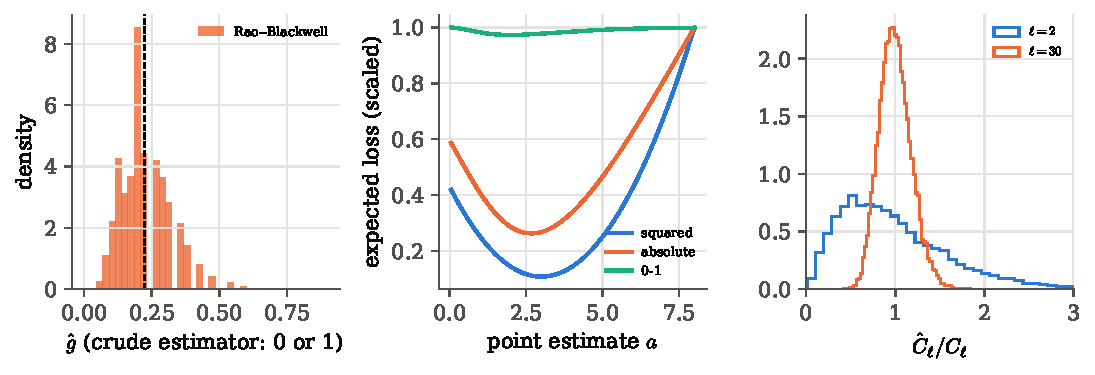
\includegraphics[width=12.5cm]{figures/ch03/estimator_recipe.pdf}
\caption{Three outcomes of the recipe. Left: the Rao--Blackwellised estimate of
$e^{-\lambda}$ over $20\,000$ experiments; the crude estimator can only
answer $0$ or $1$, while the averaged one is tightly peaked on the truth
(dashed). Middle: expected loss for a skewed posterior as a function of the
announced value, for squared, absolute and zero--one loss. Their minima are
at the mean, the median and the mode, from right to left. Right: the maximum-likelihood
$\Chat/\Cell$ from $20\,000$ skies at $\ell=2$ and $\ell=30$, centred on the
truth with widths set by cosmic variance.}
\label{3b:fig:recipe}
\end{figure}

\begin{taxonomy}[Which estimator when]
\small
\begin{tabular}{@{}>{\raggedright\arraybackslash}p{3.7cm}>{\raggedright\arraybackslash}p{3.9cm}>{\raggedright\arraybackslash}p{4.0cm}@{}}
  situation & estimator & why\\
  \hline
  exponential family (Poisson, exponential, Gaussian, $\chi^2_\nu$-type)
    & maximum likelihood $=$ match the mean of the sufficient statistic
    & sufficient, efficient, on the Cram\'er--Rao floor for the mean parameter\\[2pt]
  Gaussian noise, known $\Cmat$
    & least squares (weights $\Cmat^{-1}$)
    & it is the ML estimator; exact for linear models\\[2pt]
  counts in bins
    & Poisson ML ($2\sum[\mu-n\ln\mu]$), not $\sqrt n$-weighted $\chi^2$
    & no bias on the normalisation, valid for small counts\\[2pt]
  Gaussian isotropic sky
    & $\Chat=\frac1{2\ell+1}\sum_m|\alm|^2$
    & ML, unbiased, attains cosmic variance\\[2pt]
  a crude unbiased estimator exists
    & average it over a sufficient statistic
    & never increases the variance (Rao--Blackwell)\\[2pt]
  prior information, or a cost of error
    & Bayes: posterior mean, median or mode
    & minimises the expected squared, absolute, 0--1 loss\\[2pt]
  intractable likelihood, masks, non-Gaussian summaries
    & simple statistic, bias and covariance calibrated by simulation
    & honest error bar, not optimal\\
\end{tabular}
\end{taxonomy}
\providecommand{\ThreeBHNaiveMean}{}\renewcommand{\ThreeBHNaiveMean}{69.49}
\providecommand{\ThreeBHNaiveBias}{}\renewcommand{\ThreeBHNaiveBias}{-0.5076}
\providecommand{\ThreeBHNaiveSd}{}\renewcommand{\ThreeBHNaiveSd}{0.6265}
\providecommand{\ThreeBHNaiveRmse}{}\renewcommand{\ThreeBHNaiveRmse}{0.8063}
\providecommand{\ThreeBHRatioMean}{}\renewcommand{\ThreeBHRatioMean}{70.24}
\providecommand{\ThreeBHRatioBias}{}\renewcommand{\ThreeBHRatioBias}{0.2388}
\providecommand{\ThreeBHRatioSd}{}\renewcommand{\ThreeBHRatioSd}{0.5362}
\providecommand{\ThreeBHRatioRmse}{}\renewcommand{\ThreeBHRatioRmse}{0.587}
\providecommand{\ThreeBHMLMean}{}\renewcommand{\ThreeBHMLMean}{70.03}
\providecommand{\ThreeBHMLBias}{}\renewcommand{\ThreeBHMLBias}{0.02722}
\providecommand{\ThreeBHMLSd}{}\renewcommand{\ThreeBHMLSd}{0.5191}
\providecommand{\ThreeBHMLRmse}{}\renewcommand{\ThreeBHMLRmse}{0.5198}
\providecommand{\ThreeBHNaiveBiasLead}{}\renewcommand{\ThreeBHNaiveBiasLead}{-0.4992}
\providecommand{\ThreeBHNaiveBiasTh}{}\renewcommand{\ThreeBHNaiveBiasTh}{-0.5181}
\providecommand{\ThreeBHRatioBiasLead}{}\renewcommand{\ThreeBHRatioBiasLead}{0.1672}
\providecommand{\ThreeBHRatioBiasTh}{}\renewcommand{\ThreeBHRatioBiasTh}{0.2376}
\providecommand{\ThreeBHaBias}{}\renewcommand{\ThreeBHaBias}{7.845\times10^{-4}}
\providecommand{\ThreeBHaSd}{}\renewcommand{\ThreeBHaSd}{0.0161}
\providecommand{\ThreeBHaSdTh}{}\renewcommand{\ThreeBHaSdTh}{0.01611}
\providecommand{\ThreeBHMLSdTh}{}\renewcommand{\ThreeBHMLSdTh}{0.5192}
\providecommand{\ThreeBHMLBiasTh}{}\renewcommand{\ThreeBHMLBiasTh}{0.001926}
\providecommand{\ThreeBHMLBiasCorr}{}\renewcommand{\ThreeBHMLBiasCorr}{0.02529}
\providecommand{\ThreeBHMLMedianBias}{}\renewcommand{\ThreeBHMLMedianBias}{0.02696}
\providecommand{\ThreeBHCovOne}{}\renewcommand{\ThreeBHCovOne}{0.6853}
\providecommand{\ThreeBHCovTwo}{}\renewcommand{\ThreeBHCovTwo}{0.948}
\providecommand{\ThreeBHaBiasLin}{}\renewcommand{\ThreeBHaBiasLin}{7.927\times10^{-4}}
\providecommand{\ThreeBHmagLowZ}{}\renewcommand{\ThreeBHmagLowZ}{0.2173}
\providecommand{\ThreeBHmagHighZ}{}\renewcommand{\ThreeBHmagHighZ}{0.02173}
\providecommand{\ThreeBHNaiveBiasFour}{}\renewcommand{\ThreeBHNaiveBiasFour}{-0.5158}
\providecommand{\ThreeBHRatioBiasFour}{}\renewcommand{\ThreeBHRatioBiasFour}{0.2403}
\providecommand{\ThreeBHMLBiasFour}{}\renewcommand{\ThreeBHMLBiasFour}{0.02787}
\providecommand{\ThreeBHMLSdFour}{}\renewcommand{\ThreeBHMLSdFour}{0.2588}
\providecommand{\ThreeBHCalSd}{}\renewcommand{\ThreeBHCalSd}{1.104}
\providecommand{\ThreeBHCalSdTh}{}\renewcommand{\ThreeBHCalSdTh}{1.098}
\providecommand{\ThreeBHCalCovOne}{}\renewcommand{\ThreeBHCalCovOne}{0.6798}
\providecommand{\ThreeBHCalCovNaive}{}\renewcommand{\ThreeBHCalCovNaive}{0.3605}
\providecommand{\ThreeBHsigM}{}\renewcommand{\ThreeBHsigM}{0.03}
\providecommand{\ThreeBHOneML}{}\renewcommand{\ThreeBHOneML}{70.19}
\providecommand{\ThreeBHOneSd}{}\renewcommand{\ThreeBHOneSd}{0.5231}
\providecommand{\ThreeBHFishDet}{}\renewcommand{\ThreeBHFishDet}{0}
\providecommand{\ThreeBHsaCal}{}\renewcommand{\ThreeBHsaCal}{0.03409}
\providecommand{\ThreeBHsaStat}{}\renewcommand{\ThreeBHsaStat}{0.01618}
\providecommand{\ThreeBHCambDiff}{}\renewcommand{\ThreeBHCambDiff}{8.326\times10^{-5}}
\providecommand{\ThreeBHCambOm}{}\renewcommand{\ThreeBHCambOm}{0.3152}
\providecommand{\ThreeBHhzMean}{}\renewcommand{\ThreeBHhzMean}{69.99}
\providecommand{\ThreeBHhzSd}{}\renewcommand{\ThreeBHhzSd}{0.6258}
\providecommand{\ThreeBOmhzMean}{}\renewcommand{\ThreeBOmhzMean}{0.3006}
\providecommand{\ThreeBOmhzSd}{}\renewcommand{\ThreeBOmhzSd}{0.02365}
\providecommand{\ThreeBHhzSdTh}{}\renewcommand{\ThreeBHhzSdTh}{0.6333}
\providecommand{\ThreeBHhzSdFixed}{}\renewcommand{\ThreeBHhzSdFixed}{0.2811}
\providecommand{\ThreeBOmhzSdTh}{}\renewcommand{\ThreeBOmhzSdTh}{0.02399}
\providecommand{\ThreeBHhzRho}{}\renewcommand{\ThreeBHhzRho}{-0.8957}
\providecommand{\ThreeBHhzTwoD}{}\renewcommand{\ThreeBHhzTwoD}{70.79}
\providecommand{\ThreeBHhzProf}{}\renewcommand{\ThreeBHhzProf}{70.79}
\providecommand{\ThreeBOmhzTwoD}{}\renewcommand{\ThreeBOmhzTwoD}{0.2878}
\providecommand{\ThreeBOmhzProf}{}\renewcommand{\ThreeBOmhzProf}{0.2878}
\providecommand{\ThreeBHqZero}{}\renewcommand{\ThreeBHqZero}{-0.55}
\providecommand{\ThreeBHlawBiasTen}{}\renewcommand{\ThreeBHlawBiasTen}{-2.965}
\providecommand{\ThreeBHlawBiasFive}{}\renewcommand{\ThreeBHlawBiasFive}{-1.687}
\providecommand{\ThreeBHqBiasTen}{}\renewcommand{\ThreeBHqBiasTen}{0.1555}
\providecommand{\ThreeBHqBiasFiveH}{}\renewcommand{\ThreeBHqBiasFiveH}{2.873}
\providecommand{\ThreeBHlawSigTen}{}\renewcommand{\ThreeBHlawSigTen}{0.5192}
\providecommand{\ThreeBHlawZcross}{}\renewcommand{\ThreeBHlawZcross}{0.02}
\providecommand{\ThreeBHqZcross}{}\renewcommand{\ThreeBHqZcross}{0.192}
\providecommand{\ThreeBHlawBiasMCTen}{}\renewcommand{\ThreeBHlawBiasMCTen}{-2.988}
\providecommand{\ThreeBHlawBiasMCThirty}{}\renewcommand{\ThreeBHlawBiasMCThirty}{-7.16}
\providecommand{\ThreeBHlawBiasThirty}{}\renewcommand{\ThreeBHlawBiasThirty}{-7.171}
\providecommand{\ThreeBHTrue}{}\renewcommand{\ThreeBHTrue}{70}
\providecommand{\ThreeBHMtrue}{}\renewcommand{\ThreeBHMtrue}{-19.25}
\providecommand{\ThreeBHsigInt}{}\renewcommand{\ThreeBHsigInt}{0.15}
\providecommand{\ThreeBHsigV}{}\renewcommand{\ThreeBHsigV}{300}
\providecommand{\ThreeBHN}{}\renewcommand{\ThreeBHN}{100}
\providecommand{\ThreeBHNmock}{}\renewcommand{\ThreeBHNmock}{20000}
\providecommand{\ThreeBHNhz}{}\renewcommand{\ThreeBHNhz}{300}
\providecommand{\ThreeBHNmockhz}{}\renewcommand{\ThreeBHNmockhz}{1000}
\providecommand{\ThreeBHKappaSigSq}{}\renewcommand{\ThreeBHKappaSigSq}{0.004772}
\providecommand{\ThreeBCCN}{}\renewcommand{\ThreeBCCN}{30}
\providecommand{\ThreeBCCNmock}{}\renewcommand{\ThreeBCCNmock}{4000}
\providecommand{\ThreeBCCErr}{}\renewcommand{\ThreeBCCErr}{8}
\providecommand{\ThreeBCCHone}{}\renewcommand{\ThreeBCCHone}{69.74}
\providecommand{\ThreeBCCSigone}{}\renewcommand{\ThreeBCCSigone}{1.02}
\providecommand{\ThreeBCCHprofone}{}\renewcommand{\ThreeBCCHprofone}{71.02}
\providecommand{\ThreeBCCOmprofone}{}\renewcommand{\ThreeBCCOmprofone}{0.282}
\providecommand{\ThreeBCCMean}{}\renewcommand{\ThreeBCCMean}{70.02}
\providecommand{\ThreeBCCMeanErr}{}\renewcommand{\ThreeBCCMeanErr}{0.02}
\providecommand{\ThreeBCCSd}{}\renewcommand{\ThreeBCCSd}{1.019}
\providecommand{\ThreeBCCBound}{}\renewcommand{\ThreeBCCBound}{1.022}
\providecommand{\ThreeBCCProfMean}{}\renewcommand{\ThreeBCCProfMean}{69.95}
\providecommand{\ThreeBCCProfSd}{}\renewcommand{\ThreeBCCProfSd}{3.08}
\providecommand{\ThreeBCCOmSd}{}\renewcommand{\ThreeBCCOmSd}{0.041}
 
\section{A worked problem: finding the estimator of the Hubble constant}
\label{3b:sec:hubble}

A white dwarf in a binary system accretes matter from its companion until it
approaches the Chandrasekhar mass, and then it explodes. The explosion, a
type~Ia supernova, is nearly the same every time: after a correction for how
fast its light curve declines, its peak luminosity varies from one supernova
to the next by only about $15\%$. That makes it a \newterm{standard candle}
\unpack{an object whose true brightness is known, so its apparent brightness
tells us its distance}. A spectrum of the host galaxy gives its redshift $z$
to a few parts in $10^5$. The peak apparent brightness, measured as a
magnitude $m$, is known far less well: the intrinsic spread and the
photometry together scatter it by about $0.15$ magnitudes.

A survey collects $N$ pairs $(z_i,m_i)$. Nearby galaxies recede with
velocities proportional to their distances, and the constant of
proportionality is the Hubble constant $H_0$. So the pairs contain $H_0$.
The obvious way to get it out is the one Hubble used: turn each magnitude
into a distance, plot velocity against distance, and fit a straight line
through the origin. That obvious estimator is wrong. For a survey of $100$
supernovae its slope is too low by about half a km/s/Mpc, as large as its
own error bar, and the offset does not shrink when the survey grows to
$400$ or $4000$ supernovae. A different function of the same pairs has no
offset and the smallest error bar any estimator can have. It comes out of
the five-step procedure of \cref{3b:sec:recipe}: write the likelihood, find
the sufficient statistic, build candidates, compare them with the
Cram\'er--Rao bound, and simulate when formulas run out.
The same constant returns several times later, each time reached by a different route: the distance
ladder that supplies the supernova luminosity these mock surveys take as known
(\cref{T2b:sec:ladder}) and its disagreement with the CMB (\cref{T2b:sec:tension}), the baryon
acoustic ruler read backwards as an inverse ladder (\cref{T2b:sec:bao}), a CMB chain reweighted by the
ladder value (\cref{9c:sec:importance}), the CMB forecast in which $H_0$ is a derived parameter
(\cref{10a:sec:cmb-planck}), cosmic chronometers that need no calibration at all
(\cref{3b:sec:hubble-cc,11c:sec:cc}), and the peculiar velocities of the local flow
(\cref{11c:sec:virgo,11c:sec:cosmicvar}); \cref{11c:sec:h0-routes} brings them together.

\paragraph{The question.}
Given redshifts $z_i$ and apparent magnitudes $m_i$ of $N$ supernovae,
\begin{enumerate}
  \item where does the noise live, and what is the likelihood?
  \item which function of the data is an unbiased estimator of $H_0$ with the
        smallest scatter, and what is its error bar?
  \item what can supernovae alone \emph{not} tell us about $H_0$?
  \item what changes when the supernovae are far enough away that the Hubble
        law is no longer a straight line?
\end{enumerate}

\subsection{Step 1: the model, and where the noise lives}
\label{3b:sec:hubble-model}

Two standard results of cosmology are the physical inputs. The first is the
\newterm{Hubble law}: at low redshift the
recession velocity $cz$ of a galaxy is proportional to its distance $d$,
\[
  cz=H_0\,d .
\]
A galaxy also moves through space with a \newterm{peculiar velocity}
\unpack{its velocity relative to the smooth expansion, caused by the pull of
nearby structure}. Along the line of sight this adds a random velocity
$v_i$ to the recession velocity. Its spread is $\sigma_v\approx300$~km/s, so
that for galaxy $i$
\begin{equation}
  cz_i=H_0\,d_i+v_i,\qquad v_i\sim\Normal(0,\sigma_v^2).
  \label{3b:eq:hubble-law}
\end{equation}
The second piece is the \newterm{distance modulus}: the apparent magnitude
$m$ and the absolute magnitude $M$ (the magnitude the object would have at
$10$~pc) differ by
\[
  \mu\equiv m-M=5\log_{10}\frac{D_L}{10\,\text{pc}}
  =5\log_{10}\frac{D_L}{\text{Mpc}}+25 ,
\]
where $D_L$ is the luminosity distance \unpack{the distance for which the
observed flux is $L/4\pi D_L^2$}. At low redshift $D_L=d$. The $+25$ is
$5\log_{10}(10^6\,\text{pc}/10\,\text{pc})$, the price of measuring distances
in Mpc. Magnitudes are logarithmic and run backwards: $5$ magnitudes fainter
means $100$ times less flux, and a larger $m$ means a larger distance. From
now on $d$ is in Mpc, velocities are in km/s and $H_0$ is in km/s/Mpc.

\paragraph{The noise is Gaussian in the magnitude.}
The luminosity of a supernova scatters by a fixed \emph{fraction} from one
explosion to the next, and the photometry measures fluxes with a fixed
fractional error. On a logarithmic scale a fixed fraction is a fixed
additive amount, so the scatter is an additive Gaussian noise in the
magnitude:
\begin{equation}
  m_i=M+5\log_{10}d_i+25+\epsilon_i,\qquad \epsilon_i\sim\Normal(0,\sigma_{\rm int}^2),
  \label{3b:eq:sn-mag}
\end{equation}
with $\sigma_{\rm int}=\ThreeBHsigInt$~mag, the combined intrinsic and
measurement scatter. The noise $\epsilon_i$ is independent of the peculiar
velocity $v_i$. The distance ``measured'' from the magnitude is
\begin{equation}
  \tilde d_i\equiv10^{(m_i-M-25)/5}=d_i\,10^{\epsilon_i/5}=d_i\,e^{\kappa\epsilon_i},
  \qquad\kappa\equiv\frac{\ln10}{5}\approx0.4605 .
  \label{3b:eq:dtilde}
\end{equation}
A Gaussian in the exponent makes $\tilde d_i$ \newterm{log-normal}
\unpack{its logarithm, not itself, is Gaussian}. Its median is the true $d_i$,
since $\epsilon_i$ is positive or negative with equal probability, but its
mean is not. All the moments follow from one Gaussian integral, which we
shall use repeatedly. For $\epsilon\sim\Normal(0,\sigma^2)$ and any real $t$,
\begin{align}
  \E\,e^{t\epsilon}
  &=\int_{-\infty}^{\infty}\frac{\dd\epsilon}{\sqrt{2\pi}\sigma}\,
    e^{t\epsilon-\epsilon^2/2\sigma^2}
   \eqby{1}\int_{-\infty}^{\infty}\frac{\dd\epsilon}{\sqrt{2\pi}\sigma}\,
    e^{-(\epsilon-t\sigma^2)^2/2\sigma^2+t^2\sigma^2/2}
   \eqby{2}e^{t^2\sigma^2/2} .
  \label{3b:eq:lognormal-mgf}
\end{align}
\begin{explain}
  \item Complete the square:
        $t\epsilon-\epsilon^2/2\sigma^2=-(\epsilon-t\sigma^2)^2/2\sigma^2+t^2\sigma^2/2$.
  \item The remaining integrand is a normalised Gaussian centred on $t\sigma^2$,
        which integrates to one.
\end{explain}
With $t=\kappa$ and $t=2\kappa$,
\begin{equation}
  \E\,\tilde d_i=d_i\,e^{\kappa^2\sigma_{\rm int}^2/2},
  \qquad
  \E\,\tilde d_i^{\,2}=d_i^2\,e^{2\kappa^2\sigma_{\rm int}^2},
  \qquad
  \E\,\tilde d_i^{\,-1}=d_i^{-1}\,e^{\kappa^2\sigma_{\rm int}^2/2}.
  \label{3b:eq:dtilde-moments}
\end{equation}
For $\sigma_{\rm int}=\ThreeBHsigInt$~mag, $\kappa^2\sigma_{\rm int}^2=\ThreeBHKappaSigSq$:
the average distance built from magnitudes is too large by a quarter of a
percent, and the average of its square by one percent. Both the distance
and its inverse are biased \emph{upwards}. These small factors are the whole
story of the first two candidates below.

\paragraph{The likelihood, in the variable where the noise lives.}
The redshifts are measured almost exactly, so we condition on them and let
the noise sit in $m_i$. Write $x_i\equiv v_i/cz_i$ for the fractional
peculiar velocity. Solving \eqref{3b:eq:hubble-law} for $d_i$ and putting it
into \eqref{3b:eq:sn-mag},
\begin{align}
  m_i&\eqby{1}M+25+5\log_{10}\frac{cz_i(1-x_i)}{H_0}+\epsilon_i\nonumber\\
     &\eqby{2}M+25+5\log_{10}(cz_i)-5\log_{10}H_0+\frac{5}{\ln10}\ln(1-x_i)+\epsilon_i\nonumber\\
     &\eqby{3}M+25+5\log_{10}(cz_i)-a-\frac{5}{\ln10}\,x_i+\epsilon_i+O(x_i^2),
     \qquad a\equiv5\log_{10}H_0 .
  \label{3b:eq:sn-model}
\end{align}
\begin{explain}
  \item $d_i=(cz_i-v_i)/H_0=cz_i(1-x_i)/H_0$.
  \item The logarithm of a product is a sum of logarithms, and
        $\log_{10}y=\ln y/\ln10$.
  \item $\ln(1-x)=-x+O(x^2)$. Even at $z=0.01$, $cz=3000$~km/s and
        $\sigma_v/cz=0.1$, so the neglected term is small.
\end{explain}
The parameter $H_0$ enters only through $a=5\log_{10}H_0$, and it enters
\emph{additively}: in the variable where the noise is Gaussian, the model is
a constant shift. The two noise terms are independent Gaussians, so their sum
is Gaussian with the sum of the variances. This is linear error propagation
(\cref{3a:sec:linear-propagation}) of the velocity $v_i$ through the factor
$\partial m_i/\partial v_i=-(5/\ln10)/cz_i$:
\begin{equation}
  \sigma_i^2=\sigma_{\rm int}^2+\Bigl(\frac{5}{\ln10}\,\frac{\sigma_v}{cz_i}\Bigr)^2 .
  \label{3b:eq:sn-sigma}
\end{equation}
The peculiar-velocity term is $\ThreeBHmagLowZ$~mag at $z=0.01$, larger than the
intrinsic scatter, and $\ThreeBHmagHighZ$~mag at $z=0.1$, where it is
negligible. The very nearest supernovae are the least useful for $H_0$,
because their own motions are a large fraction of their recession
velocities. The data are the model plus noise, as in
\eqref{3b:eq:model-noise}, and the likelihood is the probability of the noise
realisation $m_i-\text{prediction}_i$ that the data require:
\begin{equation}
  \ln\Like(a,M)=-\frac12\sum_{i=1}^N\frac{\bigl[m_i-M-25-5\log_{10}(cz_i)+a\bigr]^2}{\sigma_i^2}
  +\text{const}.
  \label{3b:eq:hubble-like}
\end{equation}
\Cref{3b:fig:hubble-mock} shows one simulated survey of $\ThreeBHN$
supernovae with $0.01<z<0.1$, drawn from $H_0=\ThreeBHTrue$ and
$M=\ThreeBHMtrue$ in a universe where \eqref{3b:eq:hubble-law} is exact. In
the velocity--distance plane the points fan out as the distance grows,
because a fixed magnitude error is a fixed \emph{fractional} distance error.
In the magnitude residuals the scatter is the same at all redshifts except
the nearest, where the peculiar velocities widen the band
\eqref{3b:eq:sn-sigma}.

\begin{figure}[htbp]
\centering
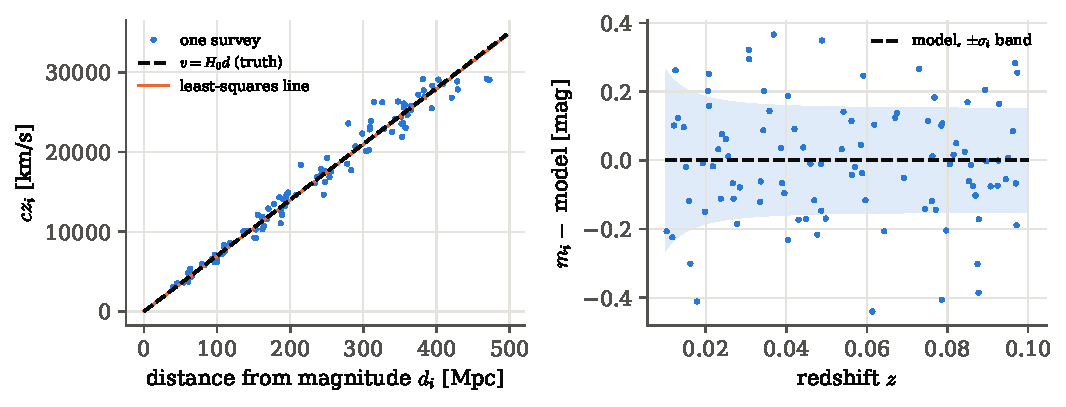
\includegraphics[width=12.5cm]{figures/ch03/hubble_mock.pdf}
\caption{One mock survey of $100$ supernovae. Left: recession velocity
against the distance inferred from each magnitude, with the true Hubble line
(dashed) and the least-squares line through the origin, which lies slightly
below it. The scatter grows in proportion to the distance. Right: the
magnitudes minus the model prediction at the true parameters. The noise is
Gaussian in this variable, with a width (shaded, $\pm\sigma_i$) that is
constant except at the lowest redshifts, where peculiar velocities add to
it.}
\label{3b:fig:hubble-mock}
\end{figure}

\subsection{Steps 2 and 3: the sufficient statistic and three candidates}
\label{3b:sec:hubble-candidates}

For the moment, pretend that the absolute magnitude $M$ of a type~Ia
supernova is known exactly. (It is not, and \cref{3b:sec:hubble-degeneracy}
shows that this changes everything about the error bar.) Each supernova
then gives its own estimate of $a=5\log_{10}H_0$,
\begin{equation}
  y_i\equiv M+25+5\log_{10}(cz_i)-m_i,
  \qquad \E\,y_i=a,\quad\Var y_i=\sigma_i^2 ,
  \label{3b:eq:sn-yi}
\end{equation}
by reading \eqref{3b:eq:sn-model} backwards. The likelihood
\eqref{3b:eq:hubble-like} is $\ln\Like=-\frac12\sum_iw_i(y_i-a)^2$ with the
weights $w_i\equiv1/\sigma_i^2$.

\paragraph{Step 2: the sufficient statistic.}
Let $W\equiv\sum_iw_i$ and $\bar y_w\equiv\sum_iw_iy_i/W$, the
inverse-variance weighted mean of the $y_i$. Then
\begin{align}
  \sum_iw_i(y_i-a)^2
  &\eqby{1}\sum_iw_i\bigl[(y_i-\bar y_w)+(\bar y_w-a)\bigr]^2\nonumber\\
  &\eqby{2}\sum_iw_i(y_i-\bar y_w)^2+2(\bar y_w-a)\sum_iw_i(y_i-\bar y_w)+W(\bar y_w-a)^2\nonumber\\
  &\eqby{3}\sum_iw_i(y_i-\bar y_w)^2+W(\bar y_w-a)^2 .
  \label{3b:eq:sn-split}
\end{align}
\begin{explain}
  \item Add and subtract $\bar y_w$.
  \item Expand the square; $\bar y_w-a$ does not depend on $i$.
  \item $\sum_iw_i(y_i-\bar y_w)=W\bar y_w-W\bar y_w=0$.
\end{explain}
So $\Like(a)=\exp[-W(\bar y_w-a)^2/2]\times\exp[-\sum_iw_i(y_i-\bar y_w)^2/2]$.
The first factor is the $g(U,a)$ of the factorisation theorem
(\cref{3b:sec:recipe-suff}) with $U=\bar y_w$, and the second is an $h(\data)$
that knows nothing about $a$. The weighted mean $\bar y_w$ is sufficient for
$a$, hence for $H_0=10^{a/5}$. Every estimator that is not a function of
$\bar y_w$ uses part of the data that carries no information about $H_0$,
and pays for it in variance or bias.

\paragraph{Candidate (a): fit the Hubble line to distances.}
Put $v_i\equiv cz_i$ on the vertical axis and the magnitude distances
$\tilde d_i$ of \eqref{3b:eq:dtilde} on the horizontal one, and minimise
$\sum_i(v_i-H\tilde d_i)^2$. Setting the derivative
$-2\sum_i\tilde d_i(v_i-H\tilde d_i)$ to zero,
\begin{equation}
  \hat H_{\rm naive}=\frac{\sum_iv_i\tilde d_i}{\sum_i\tilde d_i^{\,2}} .
  \label{3b:eq:h-naive}
\end{equation}
This is least squares, but for a model in which the noise sits in $v$ and the
horizontal coordinate is exact. Here the horizontal coordinate carries the
larger noise. For a large survey the numerator and the denominator, divided
by $N$, each converge to their means by the law of large numbers, so
$\hat H_{\rm naive}$ converges to the ratio of the means. With
$d_i=cz_i(1-x_i)/H_0$ and $\epsilon_i$ independent of $x_i$,
\begin{align}
  \E\bigl[v_i\tilde d_i\bigr]
  &\eqby{1}cz_i\,\E[d_i]\,\E\bigl[e^{\kappa\epsilon_i}\bigr]
   \eqby{2}\frac{(cz_i)^2}{H_0}\,e^{\kappa^2\sigma_{\rm int}^2/2},\nonumber\\
  \E\bigl[\tilde d_i^{\,2}\bigr]
  &\eqby{3}\E[d_i^2]\,\E\bigl[e^{2\kappa\epsilon_i}\bigr]
   \eqby{4}\frac{(cz_i)^2+\sigma_v^2}{H_0^2}\,e^{2\kappa^2\sigma_{\rm int}^2},\nonumber\\
  \hat H_{\rm naive}
  &\;\xrightarrow{N\to\infty}\;
   \frac{\sum_i\E[v_i\tilde d_i]}{\sum_i\E[\tilde d_i^{\,2}]}
   \eqby{5}H_0\,e^{-3\kappa^2\sigma_{\rm int}^2/2}\;
   \frac{\sum_i(cz_i)^2}{\sum_i\bigl[(cz_i)^2+\sigma_v^2\bigr]} .
  \label{3b:eq:naive-bias}
\end{align}
\begin{explain}
  \item $v_i=cz_i$ is fixed; $\tilde d_i=d_ie^{\kappa\epsilon_i}$ and the two
        factors are independent.
  \item $\E d_i=cz_i/H_0$ since $\E x_i=0$, and \eqref{3b:eq:lognormal-mgf}
        with $t=\kappa$.
  \item As in (1), with $\tilde d_i^{\,2}=d_i^2e^{2\kappa\epsilon_i}$.
  \item $\E d_i^2=(cz_i)^2\E(1-x_i)^2/H_0^2=[(cz_i)^2+\sigma_v^2]/H_0^2$,
        and \eqref{3b:eq:lognormal-mgf} with $t=2\kappa$.
  \item Divide; $e^{\kappa^2\sigma^2/2}/e^{2\kappa^2\sigma^2}=e^{-3\kappa^2\sigma^2/2}$.
\end{explain}
The limit is not $H_0$. The dominant factor, $e^{-3\kappa^2\sigma_{\rm int}^2/2}$,
gives a bias of $\ThreeBHNaiveBiasLead$~km/s/Mpc for $\sigma_{\rm int}=\ThreeBHsigInt$;
the peculiar velocities lower it a little further, to $\ThreeBHNaiveBiasTh$ for
the redshift range of the survey. The mechanism is the textbook one for noise
in the horizontal variable (``regression dilution''): the scatter of
$\tilde d_i$ inflates $\sum\tilde d_i^{\,2}$ more than it inflates
$\sum v_i\tilde d_i$, and the slope is pulled down. Because the limit
\eqref{3b:eq:naive-bias} does not involve $N$, the estimator is
\emph{inconsistent}: more supernovae make it converge faster to the wrong
number. Only the $O(1/N)$ corrections to the ratio of means depend on the
survey size.

\paragraph{Candidate (b): average the individual ratios.}
Each supernova gives its own $H_0$ as $v_i/\tilde d_i$, and we average them:
$\hat H_{\rm ratio}=\frac1N\sum_iv_i/\tilde d_i$. Each term is
\[
  \frac{v_i}{\tilde d_i}=\frac{cz_i\,e^{-\kappa\epsilon_i}}{d_i}
  =H_0\,\frac{e^{-\kappa\epsilon_i}}{1-x_i},
\]
and its mean follows from \eqref{3b:eq:lognormal-mgf} with $t=-\kappa$ and
$1/(1-x)=1+x+x^2+\dots$, so that $\E(1-x_i)^{-1}\approx1+\sigma_v^2/(cz_i)^2$:
\begin{equation}
  \E\,\hat H_{\rm ratio}\approx H_0\,e^{\kappa^2\sigma_{\rm int}^2/2}\,
  \frac1N\sum_i\Bigl[1+\frac{\sigma_v^2}{(cz_i)^2}\Bigr].
  \label{3b:eq:ratio-bias}
\end{equation}
The bias now has the opposite sign, $\ThreeBHRatioBiasLead$~km/s/Mpc from the
magnitude scatter and $\ThreeBHRatioBiasTh$ in total, because the nearest
supernovae have large $x_i$. It is again independent of $N$. The mean of
ratios is not the ratio of means, and averaging a nonlinear function of noisy
numbers averages its bias too.

\paragraph{Candidate (c): maximum likelihood.}
The score of \eqref{3b:eq:hubble-like} is
$\partial\ln\Like/\partial a=\sum_iw_i(y_i-a)=W(\bar y_w-a)$, which vanishes at
\begin{equation}
  \hat a=\bar y_w=\frac{\sum_iw_i\bigl[M+25+5\log_{10}(cz_i)-m_i\bigr]}{\sum_iw_i},
  \qquad w_i=\frac1{\sigma_i^2},
  \qquad \hat H_0=10^{\hat a/5}.
  \label{3b:eq:hubble-ml}
\end{equation}
It is the weighted mean of \cref{3a:sec:weighted}, applied to the
individual estimates $y_i$ of $a$ in the variable where their noise is
Gaussian, and it is a function of the sufficient statistic only.

\emph{Bias.} $\E\hat a=\sum_iw_i\E y_i/W=a$: unbiased, to the order of
\eqref{3b:eq:sn-model}. The neglected term, $-(5/\ln10)\ln(1-x_i)=(5/\ln10)(x_i+x_i^2/2+\dots)$,
has mean $(5/\ln10)\,\sigma_v^2/2(cz_i)^2$, which after weighting is
$\ThreeBHaBiasLin$~mag, about a twentieth of the error bar.

\emph{Variance and efficiency.} The $y_i$ are independent, so
\begin{align}
  \Var\hat a
  &\eqby{1}\frac{\sum_iw_i^2\,\Var y_i}{W^2}
   \eqby{2}\frac{\sum_iw_i}{W^2}=\frac1W,
  \qquad
  I(a)\eqby{3}-\E\frac{\partial^2\ln\Like}{\partial a^2}=\sum_iw_i=W .
  \label{3b:eq:hubble-fisher}
\end{align}
\begin{explain}
  \item The variance of a sum of independent terms is the sum of the variances,
        and a constant factor comes out squared.
  \item $w_i^2\Var y_i=w_i^2\sigma_i^2=w_i$.
  \item Differentiate the score $\sum_iw_i(y_i-a)$ once more; the result
        $-W$ is not random, so the expectation does nothing.
\end{explain}
The variance equals $1/I(a)$: the estimator sits on the Cram\'er--Rao bound
\eqref{3b:eq:cramer-rao}. The score $W(\bar y_w-a)$ is a linear function of
$\hat a$, the condition for equality. The error bar is
$\sigma_a=W^{-1/2}$, and by linear propagation through $H_0=e^{\kappa a}$,
$\sigma_{H_0}=\kappa H_0\sigma_a$.

\emph{From $a$ to $H_0$.} The invariance of maximum likelihood
(\cref{3b:sec:invariance}) makes $\hat H_0=10^{\hat a/5}$ the maximum-likelihood
estimator of $H_0$. It is not exactly unbiased, because the exponential is
convex. Expand $g(\hat a)=e^{\kappa\hat a}$ around the truth to second order
(the delta method of \cref{3a:sec:delta}, one order further):
\begin{align}
  \E\,\hat H_0
  &\eqby{1}\E\Bigl[g(a)+g'(a)(\hat a-a)+\tfrac12g''(a)(\hat a-a)^2\Bigr]
   \eqby{2}H_0\Bigl(1+\tfrac12\kappa^2\sigma_a^2\Bigr)
   \relby{3}{\approx}H_0\,e^{\kappa^2\sigma_a^2/2}.
  \label{3b:eq:hubble-delta}
\end{align}
\begin{explain}
  \item Taylor expansion of $g$; higher orders are smaller by further powers of $\sigma_a$.
  \item $g'=\kappa H_0$, $g''=\kappa^2H_0$; $\E(\hat a-a)=0$ and $\E(\hat a-a)^2=\sigma_a^2$.
  \item Because $\hat a$ is exactly Gaussian, \eqref{3b:eq:lognormal-mgf} with
        $t=\kappa$ gives the exponential exactly; the delta method gives its
        first two terms.
\end{explain}
The bias-corrected estimator is $\hat H_0\,e^{-\kappa^2\sigma_a^2/2}$. Since
$\sigma_a\to0$ as $N$ grows, the uncorrected $\hat H_0$ is consistent. For
$100$ supernovae $\sigma_a\approx\ThreeBHaSdTh$ and the bias is
$\ThreeBHMLBiasTh$~km/s/Mpc, utterly negligible. It matters when $\sigma_a$
is large: an $H_0$ from a single supernova ($\sigma_a=0.15$) is biased by
$0.24\%$, and averaging many such single-object values accumulates the
bias coherently, which is exactly what went wrong with candidate (b). The
cure is always the same: average in the variable where the noise is
Gaussian and transform once at the end. The median of $\hat H_0$ is exactly
$H_0$ (the exponential is monotonic), and the interval
$[10^{(\hat a-\sigma_a)/5},10^{(\hat a+\sigma_a)/5}]$ has exactly the coverage of
$\hat a\pm\sigma_a$.

\begin{keyidea}[The maximum-likelihood estimator of $H_0$]
Work in the variable where the noise is Gaussian. For low-redshift
supernovae with calibrated $M$ that is $a=5\log_{10}H_0$, and the
estimator is the inverse-variance weighted mean
\eqref{3b:eq:hubble-ml} of the single-object values
$M+25+5\log_{10}(cz_i)-m_i$, with $\sigma_i^2$ from \eqref{3b:eq:sn-sigma}.
It is sufficient, unbiased for $a$, on the Cram\'er--Rao bound $\sigma_a=(\sum_iw_i)^{-1/2}$,
and $10^{\hat a/5}$ is consistent for $H_0$. Converting magnitudes to
distances first gives inconsistent estimators.
\end{keyidea}

\subsection{Step 4: comparing the candidates on simulated surveys}
\label{3b:sec:hubble-mc}

The three biases \eqref{3b:eq:naive-bias}, \eqref{3b:eq:ratio-bias},
\eqref{3b:eq:hubble-delta} are large-$N$ approximations, and the claim that
the maximum-likelihood error bar is right is a statement about repeated
surveys. Both can be checked by simulating many surveys from a known truth,
which is the verification use of Monte Carlo (\cref{ch:06}).

\pyfile[firstline=40,lastline=66]{code/ch03/17_hubble_estimator.py}{Mock supernova surveys and the three estimators of $H_0$}
The function \pyname{sigma_mag} is \eqref{3b:eq:sn-sigma}. The function
\pyname{mock_lowz} draws redshifts uniformly in $0.01<z<0.1$, a peculiar
velocity for each galaxy, the true distance from \eqref{3b:eq:hubble-law}
and a magnitude from \eqref{3b:eq:sn-mag}; it generates the data from the
physics, not from the linearised likelihood, so the approximation in
\eqref{3b:eq:sn-model} is tested too. The arrays have one row per survey,
and every estimator sums over the last axis, so $\ThreeBHNmock$ surveys of
$\ThreeBHN$ supernovae are processed at once. \pyname{naive} is
\eqref{3b:eq:h-naive}, \pyname{ratio} the mean of $v_i/\tilde d_i$, and
\pyname{ml} returns $10^{\hat a/5}$, $\hat a$ and $\sigma_a=W^{-1/2}$ from
\eqref{3b:eq:hubble-ml} and \eqref{3b:eq:hubble-fisher}.

\begin{center}
\small
\begin{tabular}{@{}lcccc@{}}
\toprule
estimator & mean bias & predicted bias & scatter & rms error\\
 & [km/s/Mpc] & [km/s/Mpc] & [km/s/Mpc] & [km/s/Mpc]\\\midrule
(a) least-squares line \eqref{3b:eq:h-naive} & $\ThreeBHNaiveBias$ & $\ThreeBHNaiveBiasTh$ & $\ThreeBHNaiveSd$ & $\ThreeBHNaiveRmse$\\
(b) mean of ratios & $\ThreeBHRatioBias$ & $\ThreeBHRatioBiasTh$ & $\ThreeBHRatioSd$ & $\ThreeBHRatioRmse$\\
(c) maximum likelihood \eqref{3b:eq:hubble-ml} & $\ThreeBHMLBias$ & $\ThreeBHMLBiasTh$ & $\ThreeBHMLSd$ & $\ThreeBHMLRmse$\\
\bottomrule
\end{tabular}
\end{center}
The predicted biases are \eqref{3b:eq:naive-bias} and \eqref{3b:eq:ratio-bias}
averaged over the simulated redshifts, and for (c) the convexity term of
\eqref{3b:eq:hubble-delta}. The first two agree with the simulation to within
the $O(1/N)$ corrections: for surveys of $400$ supernovae the measured biases
are $\ThreeBHNaiveBiasFour$ and $\ThreeBHRatioBiasFour$, no smaller, while the
scatter of the maximum-likelihood estimator halves to $\ThreeBHMLSdFour$. The
least-squares line is off by about one standard deviation for $100$ supernovae
and by two for $400$. The small residual bias of (c) is not the convexity term
but the second-order peculiar-velocity term: the simulated mean of $\hat a$ is
too large by $\ThreeBHaBias$~mag, against the predicted $\ThreeBHaBiasLin$.
The scatter of $\hat a$ is $\ThreeBHaSd$ against the Cram\'er--Rao value
$\ThreeBHaSdTh$, and the interval $\hat a\pm\sigma_a$ covers the truth in a
fraction $\ThreeBHCovOne$ of the surveys ($\pm1.96\sigma_a$: $\ThreeBHCovTwo$),
as a $68\%$ and a $95\%$ interval should. \Cref{3b:fig:hubble-estimators} shows the three
sampling distributions.

\begin{figure}[htbp]
\centering
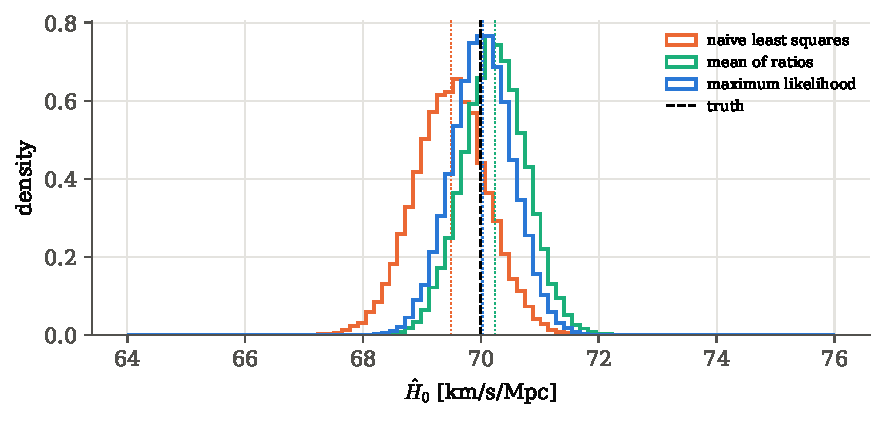
\includegraphics[width=11cm]{figures/ch03/hubble_estimators.pdf}
\caption{Sampling distributions of the three estimators of $H_0$ over
$20\,000$ mock surveys of $100$ supernovae with $H_0=70$ (dashed). The
dotted lines mark the means. The least-squares line through the magnitude
distances is shifted low and is also the widest; the mean of the individual
ratios is shifted high; the maximum-likelihood estimator is centred on the
truth and is the narrowest.}
\label{3b:fig:hubble-estimators}
\end{figure}

\subsection{What supernovae alone cannot tell us: the \texorpdfstring{$H_0$--$M$}{H0-M} degeneracy}
\label{3b:sec:hubble-degeneracy}

Look again at the likelihood \eqref{3b:eq:hubble-like}. The absolute magnitude
$M$ and $a=5\log_{10}H_0$ appear only in the combination $M-a$. Increasing
both by the same amount leaves every prediction, and so the likelihood,
unchanged. The only thing the supernovae measure is the combination
\[
  \mathcal M\equiv M-5\log_{10}H_0+25 ,
\]
which is a statement about the product ``luminosity times $H_0^{-2}$'':
brighter candles in a faster-expanding universe look exactly like fainter
candles in a slower one. In the Fisher matrix of \eqref{3b:eq:hubble-like} for
the two parameters $(M,a)$,
\begin{align}
  \Fish
  &\eqby{1}\sum_iw_i
   \begin{pmatrix}
     1 & -1\\ -1 & 1
   \end{pmatrix}
   =W\begin{pmatrix}1&-1\\-1&1\end{pmatrix},
  \qquad
  \det\Fish\eqby{2}W^2-W^2=0 ,
  \label{3b:eq:hubble-fisher2}
\end{align}
\begin{explain}
  \item $F_{jk}=-\E\,\partial^2\ln\Like/\partial\theta_j\partial\theta_k$; the
        residual is $m_i-M-25-5\log_{10}(cz_i)+a$, whose derivatives are
        $-1$ for $M$ and $+1$ for $a$, so each supernova contributes $w_i$
        times the product of the two derivatives.
  \item Determinant of the $2\times2$ matrix.
\end{explain}
A singular Fisher matrix has a zero mode: the direction $(\delta M,\delta
a)\propto(1,1)$ costs no likelihood at all, and the variance along it is
infinite. \Cref{3b:fig:hubble-degeneracy} shows this for the survey of
\cref{3b:fig:hubble-mock}. The $\Delta\chi^2$ contours in the $(M,H_0)$ plane are an
open band along $H_0\propto10^{M/5}$, and the $\chi^2$ as a function of $H_0$ at
three fixed values of $M$ has three different minima of exactly the same
depth. Evaluated numerically for that survey, $\det\Fish=\ThreeBHFishDet$ to
rounding.

The absolute magnitude must therefore come from somewhere else: from
supernovae in galaxies whose distances are measured independently, with
Cepheid variables or the tip of the red giant branch, which are in turn
calibrated geometrically with parallaxes. This is the \newterm{distance
ladder}. The distance-ladder value of $H_0$ is $73.04\pm1.04$~km/s/Mpc
\cite{Riess2022SH0ES}, while the CMB with $\Lambda$CDM gives $67.36\pm0.54$
\cite{Planck2018VI}, $4.8$ standard deviations apart: the \newterm{Hubble tension}. Since supernovae only fix
$M-5\log_{10}H_0$, the same tension can be stated as a disagreement of
$5\log_{10}(73.04/67.36)=0.18$~mag in the absolute magnitude of type~Ia supernovae.
The ladder that supplies $M$ is built as one linear model, with its error budget rung by rung, in
\cref{T2b:sec:ladder}, where the tension is also computed (\cref{T2b:sec:tension}).

\paragraph{A calibrated $M$ as a nuisance parameter.}
Suppose the calibrators give $M=M_{\rm cal}\pm\sigma_M$ with Gaussian errors.
That is one more measurement, independent of the Hubble-flow supernovae, and
its log-likelihood $-(M-M_{\rm cal})^2/2\sigma_M^2$ adds to
\eqref{3b:eq:hubble-like}. The Fisher matrix gains $1/\sigma_M^2$ in its
$MM$ element. The variance of $\hat a$, with $M$ treated as a nuisance
parameter, is the $aa$ element of the inverse:
\begin{align}
  \Fish'
  &=\begin{pmatrix}W+\sigma_M^{-2}&-W\\-W&W\end{pmatrix},
  \qquad
  \det\Fish'\eqby{1}\frac{W}{\sigma_M^2},
  \nonumber\\
  \sigma_a^2=(\Fish'^{-1})_{aa}
  &\eqby{2}\frac{W+\sigma_M^{-2}}{W/\sigma_M^2}
   \eqby{3}\frac1W+\sigma_M^2 .
  \label{3b:eq:hubble-calib}
\end{align}
\begin{explain}
  \item $(W+\sigma_M^{-2})W-W^2=W/\sigma_M^2$.
  \item The $(2,2)$ element of the inverse of a $2\times2$ matrix is its $(1,1)$
        element divided by the determinant.
  \item Divide term by term.
\end{explain}
This is the profile-likelihood variance $V_{\theta\theta}$ of
\eqref{3b:eq:profile-gauss} with $\theta=a$ and $\nu=M$: maximising the
likelihood over $M$ at each $a$ gives a parabola in $a$ of exactly this
width, and for a Gaussian likelihood marginalising over $M$ gives the same
(\cref{3b:sec:marginalise}). The two errors add in quadrature: the
statistical error of the Hubble-flow sample and the calibration error. The
estimator itself is \eqref{3b:eq:hubble-ml} with $M=M_{\rm cal}$, because
the Hubble-flow supernovae cannot move $M$ at all.

For the simulated surveys $W^{-1/2}=\ThreeBHsaStat$~mag, and with a
calibration of $\sigma_M=\ThreeBHsigM$~mag, typical of current ladders, the
total is $\sigma_a=\ThreeBHsaCal$~mag: the calibration dominates, and adding
more Hubble-flow supernovae hardly helps. In the simulation each survey
gets its own calibration $M_{\rm cal}$ drawn around the truth. The scatter of
$\hat H_0$ is then $\ThreeBHCalSd$~km/s/Mpc against the predicted
$\kappa H_0\sigma_a=\ThreeBHCalSdTh$, and the interval with the full
$\sigma_a$ covers the truth in $\ThreeBHCalCovOne$ of the surveys. Quoting only the
statistical error $W^{-1/2}$ would give intervals that cover the truth in
$\ThreeBHCalCovNaive$ of the surveys, instead of $68\%$.

\begin{figure}[htbp]
\centering
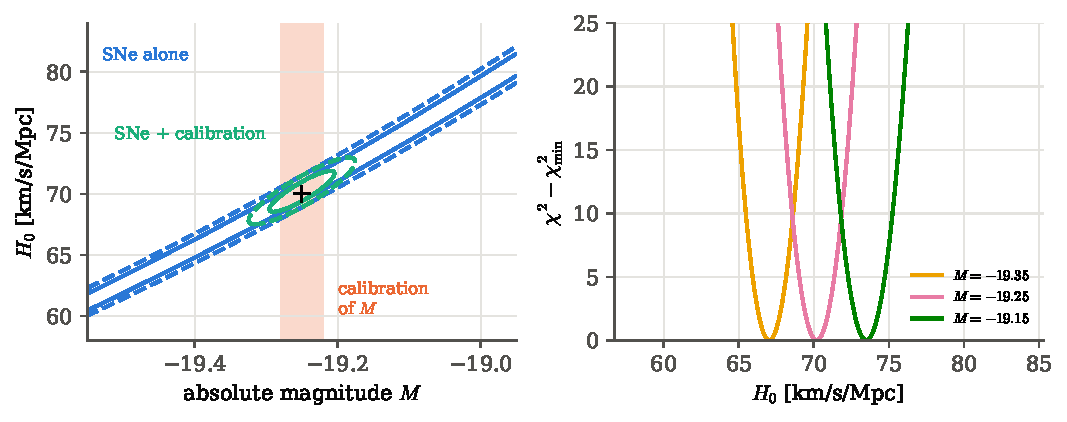
\includegraphics[width=12.5cm]{figures/ch03/hubble_degeneracy.pdf}
\caption{The degeneracy between $H_0$ and the absolute magnitude $M$ for one
survey of $100$ supernovae. Left: $\Delta\chi^2=2.30$ (solid) and $6.18$
(dashed) contours. The supernovae alone allow an open band; a calibration of $M$
to $\pm0.03$~mag (vertical strip) closes it into a small ellipse, whose
height is set mostly by the width of the strip. Right: $\chi^2$ against $H_0$
at three fixed values of $M$. Each has a perfectly good minimum of the same
depth, at a different $H_0$.}
\label{3b:fig:hubble-degeneracy}
\end{figure}

\begin{pitfall}[An error bar that forgets the calibration]
Fixing $M$ at a calibrated value and reporting the curvature error of the
Hubble-flow fit, $\kappa H_0W^{-1/2}$, conditions on the nuisance parameter
instead of profiling it. The interval is too short by the factor
$(1+W\sigma_M^2)^{-1/2}$, here about one half, and its coverage falls from
$68\%$ to about a third. The calibration error must be carried into every
number derived from the calibrated supernovae.
\end{pitfall}

\subsection{Beyond low redshift: the luminosity distance and a profile over \texorpdfstring{$\Omega_{m0}$}{Omega\_m0}}
\label{3b:sec:hubble-highz}

At larger redshift the Hubble law bends. In a flat universe with matter
density parameter $\Omega_{m0}$ and a cosmological constant, neglecting
radiation, the luminosity distance is a standard result of cosmology,
taken here as an input:
\begin{equation}
  D_L(z)=\frac{c}{H_0}\,(1+z)\int_0^z\frac{\dd z'}{E(z')},
  \qquad
  E(z)=\sqrt{\Omega_{m0}(1+z)^3+1-\Omega_{m0}} ,
  \label{3b:eq:dl}
\end{equation}
the distance travelled by light through an expanding universe whose
expansion rate is $H_0E(z)$. The model for the magnitudes becomes
$m_i=M+25+5\log_{10}(D_L(z_i)/\text{Mpc})+\text{noise}$. Write
$\bar D_L\equiv H_0D_L/c$ for the dimensionless integral, which depends on
$\Omega_{m0}$ but not on $H_0$. Then
\begin{equation}
  m_i=M+25+5\log_{10}\bigl[c\,\bar D_L(z_i;\Omega_{m0})\bigr]-a+\text{noise},
  \label{3b:eq:sn-model-dl}
\end{equation}
so $a$ still enters additively, and $M$ and $a$ are still degenerate: the
whole of \cref{3b:sec:hubble-degeneracy} carries over unchanged. What is new
is that the model depends on $\Omega_{m0}$ through an integral, nonlinearly.
The maximum-likelihood estimator is the minimum of
$\chi^2(a,\Omega_{m0})=\sum_iw_i[y_i(\Omega_{m0})-a]^2$, with
$y_i(\Omega_{m0})=M+25+5\log_{10}[c\bar D_L(z_i;\Omega_{m0})]-m_i$. At fixed
$\Omega_{m0}$ the minimum over $a$ is the weighted mean
$\hat a(\Omega_{m0})=\sum_iw_iy_i(\Omega_{m0})/W$ as before, and substituting
it leaves the profile $\chi^2_p(\Omega_{m0})=\sum_iw_i[y_i-\hat a(\Omega_{m0})]^2$,
a function of one variable that a one-dimensional minimiser handles.

\pyfile[firstline=180,lastline=184]{code/ch03/17_hubble_estimator.py}{The flat-$\Lambda$CDM luminosity distance}
\pyname{dl_bar} evaluates $\bar D_L$ by integrating $1/E$ with the trapezoidal
rule on a fine grid and interpolating at the supernova redshifts. At the
Planck 2018 best-fit parameters, it agrees with the luminosity
distance computed by CAMB to a fractional $\ThreeBHCambDiff$ out to $z=1$; CAMB
includes radiation and massive neutrinos, which is the size of the
difference.

\pyfile[firstline=207,lastline=219]{code/ch03/17_hubble_estimator.py}{Profiling $a=5\log_{10}H_0$ analytically and minimising over $\Omega_{m0}$}
The simulated surveys have $\ThreeBHNhz$ supernovae uniform in
$0.01<z<1$, with $H_0=\ThreeBHTrue$ and $\Omega_{m0}=0.3$, and $M$ known.
\pyname{profile_chi2} returns $\chi^2_p$ and $\hat a$ at one
$\Omega_{m0}$, and \pyname{minimize_scalar} finds the minimum over
$\Omega_{m0}$. For the first survey a direct two-dimensional minimisation of
$\chi^2(H_0,\Omega_{m0})$ with Nelder--Mead gives $H_0=\ThreeBHhzTwoD$,
$\Omega_{m0}=\ThreeBOmhzTwoD$, the same as the profile ($\ThreeBHhzProf$,
$\ThreeBOmhzProf$): analytic profiling over the linear parameter loses nothing.

Over $\ThreeBHNmockhz$ surveys the estimates of $H_0$ average
$\ThreeBHhzMean$ with a scatter of $\ThreeBHhzSd$~km/s/Mpc, and those of
$\Omega_{m0}$ average $\ThreeBOmhzMean$ with a scatter of $\ThreeBOmhzSd$: both
are unbiased. The Fisher matrix in $(a,\Omega_{m0})$, computed with a
numerical derivative of $5\log_{10}\bar D_L$ with respect to $\Omega_{m0}$,
predicts $\ThreeBHhzSdTh$ and $\ThreeBOmhzSdTh$. With $\Omega_{m0}$ held fixed
the $H_0$ error would be only $\ThreeBHhzSdFixed$: the two estimates are
correlated with $\rho=\ThreeBHhzRho$, and profiling over $\Omega_{m0}$ widens
the error by $1/\sqrt{1-\rho^2}$, exactly the mechanism of
\cref{3b:sec:profile-width}. A higher $\Omega_{m0}$ decelerates the expansion,
makes distant supernovae nearer and brighter, and is compensated by a lower $H_0$.

\paragraph{When does the straight Hubble law fail?}
Expanding \eqref{3b:eq:dl} in $z$ gives the distance modulus
$\mu=25+5\log_{10}(cz/H_0)+1.086\,(1-q_0)\,z+O(z^2)$, where
$1.086=5/(2\ln10)$ and $q_0$ is the deceleration parameter, $q_0=\tfrac32\Omega_{m0}-1=\ThreeBHqZero$
for flat $\Lambda$CDM. The pure Hubble law drops the linear term. Applying
the estimator \eqref{3b:eq:hubble-ml} to noiseless $\Lambda$CDM magnitudes
with redshifts up to $z_{\max}$ gives its bias directly, since the estimator
is linear in the data (\cref{3b:fig:hubble-highz}, right). For $z_{\max}=0.05$ the bias is
$\ThreeBHlawBiasFive$~km/s/Mpc, for $z_{\max}=0.1$ it is $\ThreeBHlawBiasTen$,
about six times the statistical error $\ThreeBHlawSigTen$ of $100$
supernovae. The Monte Carlo surveys confirm it: $\ThreeBHlawBiasMCTen$ at
$z_{\max}=0.1$ and $\ThreeBHlawBiasMCThirty$ at $0.3$ (predicted
$\ThreeBHlawBiasThirty$). The bias exceeds the statistical error of $100$
supernovae already for $z_{\max}\approx\ThreeBHlawZcross$. Keeping the $q_0$ term
moves this to $z_{\max}\approx\ThreeBHqZcross$, with a bias of
$\ThreeBHqBiasTen$~km/s/Mpc at $z_{\max}=0.1$ but $\ThreeBHqBiasFiveH$ at $0.5$; beyond that
only the full \eqref{3b:eq:dl} is safe. In practice the ``low-redshift''
estimator means the Hubble law with the $q_0$ term (and often the next one)
applied to $0.02\lesssim z\lesssim0.15$: the lower cut removes the supernovae
whose peculiar velocities dominate, the upper cut keeps the expansion
accurate. Like the bias of the least-squares line, this is a bias of a wrong
model, and it does not average away.

\begin{figure}[htbp]
\centering
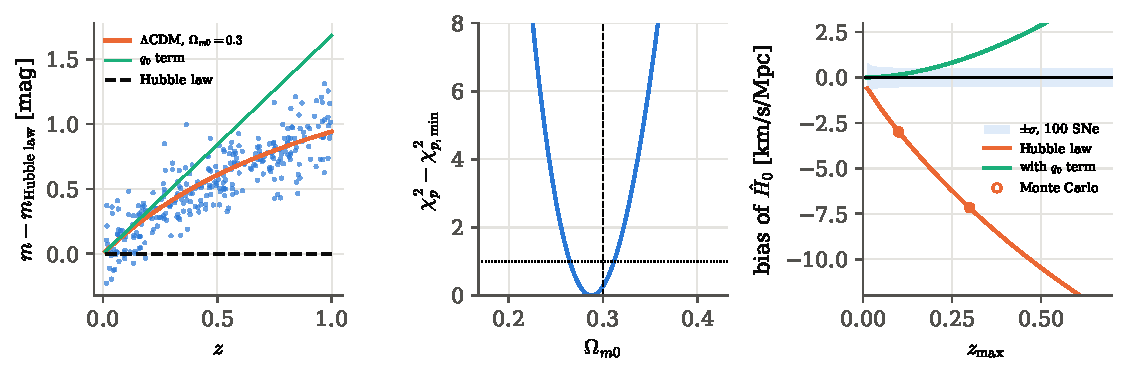
\includegraphics[width=12.8cm]{figures/ch03/hubble_highz.pdf}
\caption{Supernovae beyond the linear Hubble law. Left: one survey of $300$
supernovae to $z=1$, as magnitudes minus the Hubble-law prediction; the
$\Lambda$CDM curve follows the points, the first-order $q_0$ term follows
them only at low redshift. Middle: the profile $\chi^2_p(\Omega_{m0})$ of that
survey, with $a$ minimised analytically at each $\Omega_{m0}$; the dotted line
is $\Delta\chi^2=1$, the dashed line the truth. Right: bias of $\hat H_0$ from
fitting the pure Hubble law and the law with the $q_0$ term to supernovae up to
$z_{\max}$, compared with the $\pm1\sigma$ statistical error of $100$
supernovae (shaded); the circles are Monte Carlo checks.}
\label{3b:fig:hubble-highz}
\end{figure}

\paragraph{How the measurement is done in research.}
Real analyses solve the same problem with the same structure, on a larger
scale. The SH0ES measurement \cite{Riess2022SH0ES} writes the Cepheid
magnitudes in the anchor galaxies (with geometric distances), the Cepheids
and supernovae in the calibrator galaxies, and the Hubble-flow supernovae
($0.023<z<0.15$, with the $q_0$ and $j_0$ expansion terms) as one linear
model $\bm y=A\bm\theta+\text{noise}$ with a full covariance matrix, and
solves it by generalised least squares, $\hat{\bm\theta}=(A\T\Cmat^{-1}A)^{-1}A\T\Cmat^{-1}\bm y$
\eqref{3b:eq:normal-eq}. The parameter vector contains $M$ and $5\log_{10}H_0$
together with the Cepheid period--luminosity parameters and the host
distances, so the degeneracy of \cref{3b:sec:hubble-degeneracy} is broken
inside one fit and $\sigma_M$ is propagated automatically. The Pantheon+
analysis \cite{Brout2022PantheonPlus} fits $1550$ supernovae with a
covariance matrix that includes calibration and light-curve systematics, and
fits $M$, $H_0$ and $\Omega_{m0}$ jointly with the SH0ES calibrators, profiling or
marginalising over the light-curve standardisation parameters. Two things
our mock surveys ignored enter there: a magnitude-limited survey preferentially
finds the brighter supernovae at large distance, a selection bias that no
choice of estimator removes and that is calibrated by simulating the survey
(step~5, \cref{3b:sec:recipe-intractable}); and correlated systematics, which
are what the off-diagonal covariance is for (\cref{3b:sec:correlated}). The same
problem can be posed as Bayesian inference, with priors on
$(M,H_0,\Omega_{m0})$ and a Markov chain exploring the posterior; \cref{ch:09}
builds those chains, and \cref{9c:sec:importance} uses one to add the SH0ES value to a CMB chain by reweighting.
How the error on $H_0$ is assembled from the errors of the rungs, before any data are taken, is the
error budget of \cref{T2b:sec:ladder}, and the Fisher matrix of \cref{ch:10} returns to $H_0$ as a
parameter derived from the CMB in \cref{10a:sec:cmb-planck}.

\subsection{A second probe: cosmic chronometers, where \texorpdfstring{$H_0$}{H0} enters linearly}
\label{3b:sec:hubble-cc}

Supernovae measure distances, and the expansion rate enters only through the integral that
relates distance to $H(z)$. There is another method that measures $H(z)$ more directly.
Consider galaxies that formed their stars early in cosmic history and then stopped forming new
stars. Since no new stars are being added, their stellar populations simply grow older as the
Universe evolves, and as the stars age, the spectrum of the galaxy changes in a predictable
way. The observed spectrum can therefore be used to estimate the age of the stellar population
at a given redshift. Comparing similar passively evolving galaxies at two nearby redshifts, the
difference in their ages measures the difference in cosmic time between those redshifts, which
gives $\dd t/\dd z$. Since $1+z=a^{-1}$,
\begin{equation}
  H(z)=-\frac{1}{1+z}\,\frac{\dd z}{\dd t}=-\frac{1}{1+z}\left(\frac{\dd t}{\dd z}\right)^{-1}.
  \label{3b:eq:cc-hz}
\end{equation}
These galaxies are therefore used as \newterm{cosmic chronometers}: clocks whose age
differences give $H(z)$ without any distance.
A chronometer survey delivers $N$ triples $(z_i,H_i,\sigma_i)$: a redshift,
a measured expansion rate in km/s/Mpc, and its error bar.

\paragraph{The event, and what could have produced it.}
What we observed is the number $H_i$ at redshift $z_i$. What made it come out that way? Two
things: the true expansion rate at $z_i$, and the measurement error. In flat $\Lambda$CDM the
true rate is $H_{\rm th}(z;H_0,\Omega_{m0})=H_0\,E(z;\Omega_{m0})$, with the same $E$ as in
\eqref{3b:eq:dl}. The errors of the age measurements are independent from point to point and
Gaussian with standard deviation $\sigma_i$. So for each candidate pair $(H_0,\Omega_{m0})$ the
noise needed to turn the prediction into the data is $H_i-H_0E_i$, with $E_i\equiv E(z_i;\Omega_{m0})$,
and how plausible that noise is gives the likelihood: $-2\ln\Like=\chi^2+\text{const}$ with
\[
  \chi^2(H_0,\Omega_{m0})=\sum_{i=1}^{N}\frac{\bigl(H_i-H_0E_i\bigr)^2}{\sigma_i^2}.
\]
Here is the feature that makes the problem easy. The matter density enters $E_i$ through a
square root, nonlinearly, but $H_0$ only multiplies it: \emph{the model is linear in $H_0$}. At
fixed $\Omega_{m0}$ the $\chi^2$ is therefore a quadratic function of $H_0$, a parabola, and its
minimum can be written down. With the three sums $S_{HH}\equiv\sum_iH_i^2/\sigma_i^2$,
$S_{HE}\equiv\sum_iH_iE_i/\sigma_i^2$ and $S_{EE}\equiv\sum_iE_i^2/\sigma_i^2$,
\begin{align}
  \chi^2(H_0)
  &\eqby{1}S_{HH}-2H_0\,S_{HE}+H_0^2\,S_{EE},
  \nonumber\\
  \frac{\dd\chi^2}{\dd H_0}
  &\eqby{2}-2S_{HE}+2H_0\,S_{EE}=0
  \quad\Longrightarrow\quad
  \hat H_0=\frac{S_{HE}}{S_{EE}}=\frac{\sum_iH_iE_i/\sigma_i^2}{\sum_iE_i^2/\sigma_i^2},
  \label{3b:eq:cc-estimator}\\
  \chi^2(H_0)
  &\eqby{3}S_{EE}\bigl(H_0-\hat H_0\bigr)^2+\chi^2_{\min},
  \qquad \chi^2_{\min}=S_{HH}-\frac{S_{HE}^2}{S_{EE}} .
  \nonumber
\end{align}
\begin{explain}
  \item Expand $(H_i-H_0E_i)^2=H_i^2-2H_0H_iE_i+H_0^2E_i^2$, divide by $\sigma_i^2$ and sum;
        $H_0$ does not depend on $i$.
  \item Differentiate the quadratic; $S_{EE}>0$, so the stationary point is the minimum.
  \item Complete the square: $S_{EE}(H_0-\hat H_0)^2=S_{EE}H_0^2-2H_0S_{HE}+S_{HE}^2/S_{EE}$.
\end{explain}
No minimiser is needed. The estimator is a \emph{weighted ratio}, and it is also a weighted
mean: each point gives its own estimate $H_i/E_i$ of $H_0$, with variance $\sigma_i^2/E_i^2$,
and \eqref{3b:eq:cc-estimator} is $\sum_iw_i(H_i/E_i)/\sum_iw_i$ with the inverse variances
$w_i=E_i^2/\sigma_i^2$ as weights, exactly the weighted mean of \cref{3a:sec:weighted}.

\paragraph{Bias, variance and the bound.}
The $H_i$ are independent with $\E H_i=H_0E_i$ and $\Var H_i=\sigma_i^2$, and the $E_i$ are
fixed numbers at fixed $\Omega_{m0}$. Then
\begin{align}
  \E\,\hat H_0
  &\eqby{1}\frac{\sum_iE_i\,\E H_i/\sigma_i^2}{S_{EE}}
   \eqby{2}\frac{H_0\sum_iE_i^2/\sigma_i^2}{S_{EE}}=H_0,
  \nonumber\\
  \Var\hat H_0
  &\eqby{3}\frac{\sum_iE_i^2\,\Var H_i/\sigma_i^4}{S_{EE}^2}
   \eqby{4}\frac{S_{EE}}{S_{EE}^2}=\frac{1}{\sum_iE_i^2/\sigma_i^2},
  \nonumber\\
  I(H_0)
  &\eqby{5}\E\Bigl[\frac{\partial^2(-\ln\Like)}{\partial H_0^2}\Bigr]
   \eqby{6}\frac12\,\frac{\dd^2\chi^2}{\dd H_0^2}=S_{EE} .
  \label{3b:eq:cc-variance}
\end{align}
\begin{explain}
  \item The expectation is linear and the denominator is not random.
  \item $\E H_i=H_0E_i$.
  \item Variances of independent terms add, each multiplied by the square of its coefficient
        $E_i/(\sigma_i^2S_{EE})$.
  \item $\Var H_i=\sigma_i^2$, so each term is $E_i^2/\sigma_i^2$.
  \item The Fisher information of \cref{3b:sec:cramer-rao}.
  \item $-\ln\Like=\chi^2/2+\text{const}$, and the second derivative of the parabola, $2S_{EE}$,
        is not random, so the expectation does nothing.
\end{explain}
The estimator is unbiased and its variance is $1/I(H_0)$: it sits on the Cram\'er--Rao bound
\eqref{3b:eq:cramer-rao}, as it must, since the score
$\partial\ln\Like/\partial H_0=-\frac12\dd\chi^2/\dd H_0=S_{EE}(\hat H_0-H_0)$ is a linear function
of $\hat H_0$. The completed square in line~3 of \eqref{3b:eq:cc-estimator} says the same thing
graphically: $\chi^2$ rises by one when $H_0$ moves by $S_{EE}^{-1/2}$ from its minimum.

Compare with the supernova estimator \eqref{3b:eq:hubble-ml}. There the parameter
$a=5\log_{10}H_0$ entered the magnitudes \emph{additively}, as a shift, and the estimator was a
weighted mean of the $y_i$; here $H_0$ enters the rates \emph{multiplicatively}, as a scale, and
the estimator is a weighted ratio. Both are instances of one rule: \emph{a parameter that enters
the model linearly, with Gaussian noise, has a closed-form maximum-likelihood estimator that is
unbiased and on the Cram\'er--Rao bound.} Unlike candidate (b) of
\cref{3b:sec:hubble-candidates}, the single-point ratios $H_i/E_i$ carry no bias, because the
noise sits in the numerator only and enters linearly.

\paragraph{The matter density.}
The closed form holds at fixed $\Omega_{m0}$. The matter density is not known exactly, and it
must be profiled or marginalised. Profiling is cheap here for the same reason as for the
distant supernovae of \cref{3b:sec:hubble-highz}: at each $\Omega_{m0}$ the best $H_0$ is
$\hat H_0(\Omega_{m0})$ of \eqref{3b:eq:cc-estimator}, and substituting it leaves the profile
$\chi^2_p(\Omega_{m0})=S_{HH}-S_{HE}^2/S_{EE}$, the $\chi^2_{\min}$ of line~3, a function of one
variable for a one-dimensional minimiser. As in \cref{3b:sec:profile-width}, letting $\Omega_{m0}$
float widens the error on $H_0$, because a higher matter density raises $E(z)$ at high redshift
and is compensated by a lower $H_0$.

\paragraph{A numerical illustration.}
Script \pyname{code/ch03/18_chronometers.py} draws $\ThreeBCCN$ points uniform in $0.07<z<2$ from
$H_0=70$, $\Omega_{m0}=0.3$, with $\ThreeBCCErr\%$ errors. For one survey
(\cref{3b:fig:cc}) the closed form gives $\hat H_0=\ThreeBCCHone\pm\ThreeBCCSigone$~km/s/Mpc at
$\Omega_{m0}=0.3$. Over $\ThreeBCCNmock$ surveys the estimates average $\ThreeBCCMean\pm\ThreeBCCMeanErr$,
unbiased, and scatter by $\ThreeBCCSd$, against the bound $S_{EE}^{-1/2}=\ThreeBCCBound$. With
$\Omega_{m0}$ profiled, the first survey gives $\hat H_0=\ThreeBCCHprofone$ and
$\hat\Omega_{m0}=\ThreeBCCOmprofone$, and over the surveys the $H_0$ estimates average
$\ThreeBCCProfMean$ with a scatter of $\ThreeBCCProfSd$, three times wider than at fixed
$\Omega_{m0}$, while $\Omega_{m0}$ scatters by $\ThreeBCCOmSd$. The full chronometer analysis, with
real data, the systematic errors of stellar-population models and the comparison with
supernovae, is in \cref{11c:sec:cc}. Chronometers are the one route to $H_0$ in the book that needs
neither a calibrated candle, as the supernovae of \cref{T2b:sec:ladder} do, nor a sound horizon, as
the CMB of \cref{10a:sec:cmb-planck} and the BAO of \cref{T2b:sec:bao} do.

\begin{figure}[htbp]
\centering
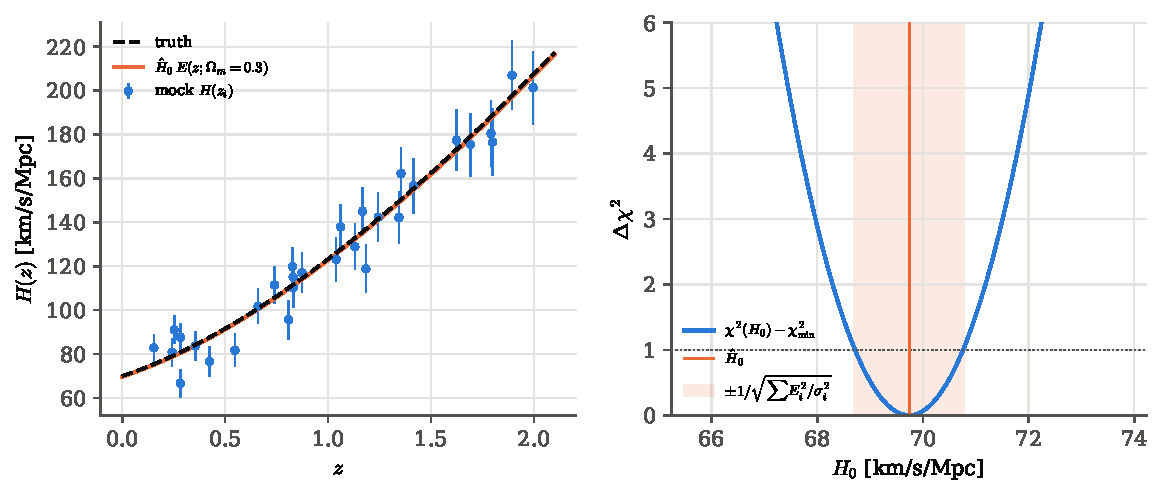
\includegraphics[width=12.8cm]{figures/ch03/chronometers.pdf}
\caption{Cosmic chronometers. Left: one mock survey of $H(z_i)$ points with their error bars,
the true expansion history (dashed) and the closed-form fit $\hat H_0E(z)$ at $\Omega_{m0}=0.3$
(orange). Right: the $\chi^2$ of that survey as a function of $H_0$ is an exact parabola; its
minimum is $\hat H_0$, and it rises by one (dotted) at $\hat H_0\pm S_{EE}^{-1/2}$ (shaded).}
\label{3b:fig:cc}
\end{figure}
\paragraph{Where this leaves us.}
The likelihood is the probability of the data, the object of \cref{ch:02}
and of \cref{3a:sec:sampling}, read backwards. For every trial value of the
parameters it asks how plausible the fluctuation is that would turn the
prediction into the data we have. Everything else follows from its shape.
Its peak is the estimate. Its width is the error bar. Its peak value,
compared with that of a saturated model, tests the fit. Maximising it over
the parameters we do not care about removes the nuisances. When no formula
is available, the bootstrap and the parametric simulation give the sampling
distribution directly. To find the best estimator, sufficiency says what the
data can tell us; candidates come from moments, maximum likelihood or a
loss function; and the Cram\'er--Rao bound and the Rao--Blackwell theorem
say when to stop improving. The full-sky power spectrum went through every
one of these steps. \Cref{ch:04} turns likelihood ratios and $\chi^2$ values into
tests and $p$-values; \cref{ch:05} multiplies the likelihood by a prior and
normalises it; \cref{ch:09} explores it with Markov chains when it has too
many dimensions to plot; \cref{ch:10} replaces it by its curvature, the
Fisher matrix, to forecast experiments before they are built.

\begin{recap}[Part 3b in one page]
\begin{itemize}
  \item Data $=$ model $+$ noise. The likelihood
        $\Like(\params)=p(\data_{\text{obs}}\given\params)$ is the probability
        (density) of the noise realisation needed to turn the prediction
        $d(\params)$ into the data. It is a function of $\params$, not a
        distribution over $\params$: no normalisation, no Jacobian, only
        ratios matter.
  \item Independent data multiply: $\ell=\sum_i\ln f(x_i;\params)$. The MLE
        solves $\partial\ell/\partial\params=0$; Newton--Raphson
        $\params\to\params-H^{-1}\bm g$ when it cannot be solved by hand.
  \item Gaussian noise: $-2\ell=\chi^2=\bm r\T\Cmat^{-1}\bm r$ (plus
        $\ln\det\Cmat$ if $\Cmat$ depends on $\params$). Linear models:
        $\hat\params=(A\T\Cmat^{-1}A)^{-1}A\T\Cmat^{-1}\bm D$ with covariance
        $(A\T\Cmat^{-1}A)^{-1}$, exactly. $\chi^2_{\min}\sim\chi^2_{N-m}$,
        mean $\dof=N-m$. Ignoring correlations keeps the fit unbiased but
        makes its error bar wrong.
  \item Counts: $-2\ell=2\sum[\mu_i-n_i\ln\mu_i]$; the fit conserves the
        total. Baker--Cousins $\chi^2_\lambda$ fits and tests; Neyman and
        Pearson $\chi^2$ bias the normalisation by $-\chi^2$ and
        $+\chi^2/2$.
  \item Error bar: $\hat\sigma=(-\ell''(\hat\theta))^{-1/2}$ or the
        $\Delta\ln\Like=\tfrac12$ crossings (better when $\ell$ is skewed).
        Why: $\Var S=-\E\ell''=I_n$, and $\hat\theta\approx\Normal(\theta,1/I_n)$.
  \item The MLE is consistent (Kullback--Leibler), equivariant
        ($\widehat{g(\theta)}=g(\hat\theta)$), asymptotically efficient:
        Cram\'er--Rao $\Var\hat\theta\ge1/I_n$ for unbiased estimators of
        regular models. Median on Gaussian data: efficiency $2/\pi$.
  \item Nuisance parameters: profile,
        $\Like_p(\theta)=\max_\nu\Like(\theta,\nu)$; its width is the full
        marginal error. Fixing $\nu$ underestimates the error by
        $\sqrt{1-\rho^2}$.
  \item Finding the estimator: write $\Like$; find the sufficient statistic
        from the factorisation $p=g(U,\theta)h(\data)$; build candidates;
        compare with $1/I_n$. In an exponential family the MLE matches the
        model mean of $U$ to its observed mean. Rao--Blackwell:
        $\E[W\given U]$ never has larger variance than an unbiased $W$.
        Bayes estimators: posterior mean, median, mode for squared,
        absolute, zero--one loss. Full-sky $\Chat=\sum_m|\alm|^2/(2\ell+1)$
        is sufficient, unbiased, and sits on the bound $2\Cell^2/(2\ell+1)$.
  \item Bootstrap: resample the data with replacement (or simulate from the
        fit) and use the scatter of the replicas. It fails for statistics
        controlled by extremes, such as the maximum.
\end{itemize}
\end{recap}

\section*{Chapter summary}
\addcontentsline{toc}{section}{Chapter summary}
\label{3b:sec:summary}

A number computed from data is a random variable, with a sampling
distribution over imagined repetitions of the experiment. The first idea
is to ask how such an estimator scatters: its bias, its variance, the
$1/\sqrt N$ law, the noise in variances and covariance matrices, the
propagation of errors through formulas, and the combination of
measurements. The second idea is to read the probability of the data
backwards, as a function of the parameters. That gives the likelihood,
which builds estimators and shows their error bars in its shape. On the
pipeline of \cref{ch:00} these are the first tools for the last arrow, from
a statistic's scatter to the physics: given the sampling distribution of a
summary, they produce a number, an error bar and a check of the fit. The
two tables list each concept, what it means operationally, and where it is
used next.

\begin{center}
\small
\renewcommand{\arraystretch}{1.15}
\begin{tabularx}{\linewidth}{@{}>{\raggedright\arraybackslash}p{3.3cm}
                               >{\raggedright\arraybackslash}X
                               >{\raggedright\arraybackslash}p{2.7cm}@{}}
\toprule
\multicolumn{3}{@{}l}{\textbf{Estimators and their errors (first half)}}\\
concept & operational meaning & used later in\\\midrule
statistical model & a family $f(x;\theta)$ of densities, one per parameter value; parametric if $\theta$ is finite-dimensional & every chapter\\
estimator, sampling distribution & a recipe $\hat\theta=g(x_1,\dots,x_N)$; its histogram over simulated repetitions of the experiment; standard error $=$ its width & \cref{ch:04,ch:06,ch:08}\\
bias, variance, MSE & centre offset and width of the sampling distribution; $\mathrm{MSE}=\mathrm{bias}^2+\mathrm{variance}$; compare estimators at several true values & \cref{ch:05,ch:10}\\
consistency & $\hat\theta\to\theta$ in probability; check that bias and variance both vanish as $N\to\infty$ & \cref{ch:09}\\
$1/\sqrt N$, LLN, CLT & $\Var\bar x=\sigma^2/N$; means become Gaussian with width $\sigma/\sqrt N$; fails for the Cauchy & \cref{ch:06,ch:07,ch:09}\\
sample variance, $N-1$ & divide by the number of residual degrees of freedom; $\Var S^2=2\sigma^4/(N-1)$ for Gaussian data & \cref{ch:04,ch:07}\\
cosmic variance & the variance of a variance: $\Var\Chat=2\Cell^2/(2\ell+1)$ & \cref{ch:07,ch:08}\\
sample covariance, Hartlap factor & $\hat\Cmat$ from $N_s$ simulations is noisy; multiply $\hat\Cmat^{-1}$ by $(N_s-p-2)/(N_s-1)$ & \cref{ch:08,ch:12}\\
error propagation & $U=A V A\T$ with the Jacobian $A$; exact for linear maps; replace by Monte Carlo near poles and for noisy denominators & \cref{ch:06,ch:10}\\
weighted mean & weights $1/\sigma_i^2$; $1/\sigma^2_{\hat\mu}=\sum1/\sigma_i^2$; check $\chi^2_{\min}\sim\chi^2_{N-1}$; correlated case $V^{-1}\bm1/(\bm1\T V^{-1}\bm1)$ & \cref{ch:04,ch:10}\\
\bottomrule
\end{tabularx}
\end{center}

\begin{center}
\small
\renewcommand{\arraystretch}{1.15}
\begin{tabularx}{\linewidth}{@{}>{\raggedright\arraybackslash}p{3.3cm}
                               >{\raggedright\arraybackslash}X
                               >{\raggedright\arraybackslash}p{2.7cm}@{}}
\toprule
\multicolumn{3}{@{}l}{\textbf{The likelihood (second half)}}\\
concept & operational meaning & used later in\\\midrule
likelihood & write the noise model, evaluate the probability of the observed data, vary $\params$; compare values only through ratios & every later chapter\\
not a density in $\theta$ & area arbitrary, no Jacobian; a prior is needed to make it a distribution & \cref{ch:05}\\
sufficiency, likelihood principle & the likelihood depends on the data only through a sufficient statistic; proportional likelihoods carry the same evidence & \cref{ch:04,ch:05,ch:07}\\
factorisation theorem, exponential family & $p=g(U,\theta)h(\data)$ identifies $U$; in $h\,e^{\eta\phi-A}$ the MLE solves $\E_{\hat\theta}\phi=\overline{\phi}$ & \cref{ch:05,ch:07}\\
Bayes estimator & minimise the posterior expected loss: mean for squared, median for absolute, mode for zero--one loss & \cref{ch:05,ch:09}\\
Rao--Blackwell, UMVUE & average a crude unbiased estimator over a sufficient statistic; with a complete statistic the result is the best unbiased estimator & \cref{ch:06}\\
MC-calibrated statistic & when $\Like$ is intractable, simulate, calibrate the mean and covariance of a simple statistic & \cref{ch:06,ch:08}\\
full-sky $\Chat$ & sufficient, unbiased, attains Cram\'er--Rao: cosmic variance $2\Cell^2/(2\ell+1)$ & \cref{ch:07,ch:08,ch:10}\\
noise lives in magnitudes & write the likelihood in the variable where the noise is Gaussian ($m$, not $d$); distances from magnitudes are log-normal, $\E\tilde d=d\,e^{\kappa^2\sigma^2/2}$ & \cref{ch:09}\\
naive vs ML estimator of $H_0$ & a line fitted to magnitude distances or a mean of ratios is biased and inconsistent; the weighted mean of $5\log_{10}H_0$ is sufficient and on the Cram\'er--Rao bound & \cref{ch:09,ch:10,T2b:sec:ladder}\\
$H_0$--$M$ degeneracy & SNe fix only $M-5\log_{10}H_0$ (singular Fisher matrix); a calibration adds $\sigma_M^2$ to $\sigma^2_{5\log_{10}H_0}$; the Hubble tension is $0.18$~mag in $M$ & \cref{T2b:sec:tension,9c:sec:importance,11c:sec:h0-routes}\\
maximum likelihood & maximise $\ell$; solve the score equation or iterate Newton--Raphson from a moment estimate & \cref{ch:04,ch:08,ch:10}\\
method of moments & match sample moments to model moments; a quick, consistent starting point & \cref{ch:06}\\
extended likelihood & multiply by $\mathrm{Poisson}(n;\nu)$ when the number of events is random & \cref{ch:04}\\
least squares & minimise $\chi^2=\bm r\T\Cmat^{-1}\bm r$; normal equations; covariance $(A\T\Cmat^{-1}A)^{-1}$ & \cref{ch:07,ch:08,ch:10}\\
goodness of fit & $\pval=\Prob(\chi^2_{N-m}\ge\chi^2_{\min})$; reduced $\chi^2\approx1\pm\sqrt{2/\dof}$ & \cref{ch:04}\\
$\Delta\chi^2$ regions & $\chi^2\le\chi^2_{\min}+\Delta\chi^2$ with $\Delta\chi^2$ from $\chi^2_m$ ($1$, $2.30$, $3.53$ for $68\%$) & \cref{ch:09,ch:10}\\
correlated and parameter-dependent noise & keep $\ln\det\Cmat(\params)$; GW: $(D-h|D-h)$ with $S_n(f)$; CMB: $\sum(2\ell+1)[\Chat/\Cell+\ln\Cell]$ & \cref{ch:07,ch:08,ch:10}\\
Poisson binned likelihood & $2\sum[\mu_i-n_i\ln\mu_i]$ (Cash); Baker--Cousins $\chi^2_\lambda$ to test; never $\sqrt{n_i}$ errors for few counts & \cref{ch:04,ch:06}\\
curvature error, $\Delta\ln\Like=\tfrac12$ & $\hat\sigma=(-\ell'')^{-1/2}$, or the two crossings of $\ell_{\max}-\tfrac12$; covariance $(-H)^{-1}$ & \cref{ch:09,ch:10}\\
score, Fisher information & $\E S=0$, $\Var S=-\E\ell''=I_n=nI$; $\hat\theta\approx\Normal(\theta,1/I_n)$ & \cref{ch:05,ch:10}\\
consistency, invariance & the MLE converges to the minimiser of the Kullback--Leibler divergence; $\widehat{g(\theta)}=g(\hat\theta)$, but bias is not invariant & \cref{ch:05,ch:09}\\
Cram\'er--Rao bound, efficiency & $\Var\hat\theta\ge1/I_n$ for unbiased estimators of regular models; attained by exponential families; fails for moving supports & \cref{ch:10}\\
profile likelihood & maximise over nuisance parameters at each $\theta$; read $\Delta\ln\Like_p=\tfrac12$; Wilks gives the coverage & \cref{ch:04,ch:05,ch:10}\\
bootstrap & resample the data with replacement (nonparametric) or simulate from the fit (parametric); Normal, pivotal and percentile intervals; fails for extremes & \cref{ch:06,ch:08,ch:12}\\
\bottomrule
\end{tabularx}
\end{center}

\subsection*{Reading the literature}

\begin{itemize}[leftmargin=1.2em,itemsep=2pt]
  \item \textbf{Main line.} \mainref{Chs.~5--6} for convergence, the law of
        large numbers, the central limit theorem, estimators, bias, variance
        and consistency; \mainref{Ch.~9} for the likelihood, maximum
        likelihood and its properties (consistency through the
        Kullback--Leibler divergence, equivariance, Fisher information,
        asymptotic normality, efficiency, the delta method, the parametric
        bootstrap), with sufficiency, the factorisation theorem, Rao--Blackwell and
        exponential families in its appendix; \mainref{Ch.~8} for the bootstrap and its
        intervals.
  \item \textbf{The physicist's version.} \srcref{Cowan}{\S\S1.6--1.7,
        Ch.~5} for error propagation and estimators; \srcref{Cowan}{Ch.~6}
        for maximum likelihood with physics examples (lifetimes, the angular
        distribution, extended and binned likelihoods, goodness of fit);
        \srcref{Cowan}{Ch.~7} for least squares, binned $\chi^2$ and the
        normalisation biases; \srcref{Cowan}{Ch.~8} for the method of
        moments.
  \item \textbf{Why least squares.} \srcref{Sivia}{\S3.5}: maximum
        likelihood and least squares as what Bayes' theorem reduces to
        under a flat prior and Gaussian noise; \srcref{Sivia}{\S2.3} for
        the weighted mean from a Gaussian posterior.
  \item \textbf{Careful derivations.} Casella and Berger give convergence
        and the delta method in \srcref{CasellaBerger}{\S5.5}, the
        likelihood principle and Birnbaum's argument in
        \srcref{CasellaBerger}{\S6.3}, maximum likelihood with restricted
        ranges and the invariance theorem in \srcref{CasellaBerger}{\S7.2.2},
        in \srcref{CasellaBerger}{\S6.2} sufficiency and the factorisation
        theorem, in \srcref{CasellaBerger}{\S7.2.3} Bayes estimators, and in
        \srcref{CasellaBerger}{\S7.3} mean squared error, the Cram\'er--Rao
        inequality with its attainment condition, and the Rao--Blackwell and
        Lehmann--Scheff\'e theorems.
  \item \textbf{Cosmology.} \srcref{HobsonBMC}{\S1.3.1} for the four
        ingredients of Bayes' theorem and why the likelihood is the least
        controversial one; \srcref{HobsonBMC}{\S2.4} for a $\chi^2$ fit as a
        Gaussian likelihood and the marginalisation of an unknown noise
        level. \srcref{Padilla}{\S\S3.3--3.8} for the likelihood ratio, the
        Hessian, $\chi^2$ goodness of fit, $\Delta\chi^2$ regions and a first
        look at the Fisher matrix.
  \item \textbf{Pictures.} \srcref{SeeingTheory}{pp.~16--18, 38--48} for
        interactive demonstrations of estimation, consistency and the
        central limit theorem.
  \item \textbf{Original papers.} The noise of inverted simulated
        covariance matrices \cite{Hartlap2007}; the Poisson statistic for
        sparse spectra \cite{Cash1979}; the likelihood-ratio $\chi^2$ for
        histograms \cite{BakerCousins1984}; the asymptotic $\chi^2$
        distribution of likelihood ratios \cite{Wilks1938}; the bootstrap
        \cite{Efron1979}.
\end{itemize}
  